\documentclass[UTF8]{book} % 使用book文档类型格式排版
\usepackage{ctex}  %加载包,因为我们在用中文写文档,所以必须加载这个包,否则不支持中文

%加入了一些针对XeTeX的改进并且加入了 \XeTeX 命令来输入漂亮的XeTeX logo
\usepackage{xltxtra}
%启用一些LaTeX中的功能
\usepackage{xunicode}

\usepackage{multicol}  %加载包
\usepackage{amsmath} % 调用公式宏包
\usepackage{amssymb} % 数学符号生成命令
\usepackage{array} % 数组和表格制作
\usepackage{booktabs} % 绘制水平表格线
\usepackage{calc} %四则运算
\usepackage{caption} % 插图和表格标题格式设置
\usepackage{fancyhdr} % 页眉页脚设置
\usepackage{graphicx} % 调用插图宏包
\usepackage{multicol} % 多栏排版
\usepackage{titlesec} % 章节标题格式设置

%%%% 目录样式 %%%%
\usepackage{titletoc}
\titlecontents{chapter}[1pt]{\vspace{.5\baselineskip}\bfseries}
    {{\thecontentslabel}\quad}{}
    {\hspace{.5em}\titlerule*[10pt]{$\cdot$}\contentspage}
\titlecontents{section}[2em]{\vspace{.25\baselineskip}\bfseries}
    {\thecontentslabel\quad}{}
    {\hspace{.5em}\titlerule*[10pt]{$\cdot$}\contentspage}

\usepackage{color}
\usepackage{xcolor} % 颜色处理
%\usepackage{indentfirst} % 自动首行缩进
%\setlength{\parindent}{2.22em} % 设置首行缩进的距离
% 设置超链接颜色
\usepackage[colorlinks=true,linkcolor=black,urlcolor=black,citecolor=black]{hyperref} % 根据章节标题生成PDF书签

%%%% 版面 %%%%
\usepackage[top=0.5in,bottom=0.5in,left=1.25in,right=0.8in]{geometry}
% 设置行距
\linespread{1}
\usepackage{lscape}
\usepackage{listings} %插入代码,代码页需要加入[fragile]
\usepackage{xeCJK}

%\usepackage[slantfont,boldfont]{xeCJK} % 允许斜体和粗体

%%%% fontspec 宏包 %%%%
\usepackage{fontspec}
% 指定字体
%\setmonofont[Mapping={}]{Monaco}	%英文引号之类的正常显示,相当于设置英文字体
%\setsansfont{Monaco} %设置英文字体 Monaco, Consolas,  Fantasque Sans Mono
%\setmainfont{Monaco} %设置英文字体
% \setCJKmainfont{方正兰亭黑简体}  %中文字体设置
% \setCJKsansfont{华康少女字体} %设置中文字体
% \setCJKmonofont{华康少女字体} %设置中文字体

%%%%%%%%%% 图形支持宏包 %%%%%%%%%%
\usepackage{graphicx}                % 嵌入png图像
\usepackage{color,xcolor}            % 支持彩色文本、底色、文本框等
%\usepackage{subfigure}
%\usepackage{epsfig}                 % 支持eps图像
%\usepackage{picinpar}               % 图表和文字混排宏包
%\usepackage[verbose]{wrapfig}       % 图表和文字混排宏包
%\usepackage{eso-pic}                % 向文档的部分页加n副图形, 可实现水印效果
%\usepackage{eepic}                  % 扩展的绘图支持
%\usepackage{curves}                 % 绘制复杂曲线
%\usepackage{texdraw}                % 增强的绘图工具
%\usepackage{treedoc}                % 树形图绘制
%\usepackage{pictex}                 % 可以画任意的图形
%\usepackage{hyperref}

%\setCJKmainfont{Kai}   % 设置缺省中文字体
%\setCJKmonofont{Hei}   % 设置等宽字体
%\setmainfont{Optima}   % 英文衬线字体
%\setmonofont{Monaco}   % 英文等宽字体
%\setsansfont{Trebuchet MS} % 英文无衬线字体

\makeatletter
\providecommand*\input@path{}
\newcommand\addinputpath[1]{
\expandafter\def\expandafter\input@path
\expandafter{\input@path{#1}}}
\addinputpath{body/}
\makeatother

\definecolor{keywordcolor}{rgb}{0.8,0.1,0.5}
\lstset{language=C++, %用于设置语言为C++
    numbers=left, %设置行号位置
    numberstyle=\tiny, %设置行号大小
    keywordstyle=\color{keywordcolor} \bfseries,
    identifierstyle=,
    basicstyle=\ttfamily,
    commentstyle=\color{blue} \textit, %注释颜色
    stringstyle=\ttfamily,
    showstringspaces=false,
    frame=shadowbox, %边框
    %frame = single,
    tabsize=2, %设置tab空格数
    showspaces=false, %不显示空格
    escapeinside=``, %逃逸字符(1左面的键),用于显示中文
    %breaklines, %自动折行
    captionpos=b
}
% \title{ACM-ICPC-Template}  %文档标题
%\author{ramay7}  % 作者
% \date{2016年10月}  %定义时间
\pagenumbering{arabic} % 页码格式是阿拉伯数字

\begin{document}

-\\
\vspace{80pt}
%^Keepaspectratio=true,
\begin{center}

\includegraphics[height = 10cm,width = 15cm]{acm.png}
\end{center}
\vspace{80pt}
\begin{center}
\Huge {ACM-ICPC Template Book} \\
\end{center}
\thispagestyle{empty}
\vspace{50pt}

\begin{titlepage}
\title{\huge {ACM-ICPC Template Book}}
\author{ramay7 \\[15pt]
Soochow University\\[10pt]
Mechanical and Electrical Engineering College}  % 作者
\date{$Oct.\ 2016$}  %定义时间
\end{titlepage}
\thispagestyle{empty} %当前页不显示页码
\maketitle

\tableofcontents % 插入目录
%\mainmatter
%\documentclass[UTF8]{book} % 使用book文档类型格式排版
\usepackage{ctex}  %加载包,因为我们在用中文写文档,所以必须加载这个包,否则不支持中文

%加入了一些针对XeTeX的改进并且加入了 \XeTeX 命令来输入漂亮的XeTeX logo
\usepackage{xltxtra}
%启用一些LaTeX中的功能
\usepackage{xunicode}

\usepackage{multicol}  %加载包
\usepackage{amsmath} % 调用公式宏包
\usepackage{amssymb} % 数学符号生成命令
\usepackage{array} % 数组和表格制作
\usepackage{booktabs} % 绘制水平表格线
\usepackage{calc} %四则运算
\usepackage{caption} % 插图和表格标题格式设置
\usepackage{fancyhdr} % 页眉页脚设置
\usepackage{graphicx} % 调用插图宏包
\usepackage{multicol} % 多栏排版
\usepackage{titlesec} % 章节标题格式设置

%%%% 目录样式 %%%%
\usepackage{titletoc}
\titlecontents{chapter}[1pt]{\vspace{.5\baselineskip}\bfseries}
    {{\thecontentslabel}\quad}{}
    {\hspace{.5em}\titlerule*[10pt]{$\cdot$}\contentspage}
\titlecontents{section}[2em]{\vspace{.25\baselineskip}\bfseries}
    {\thecontentslabel\quad}{}
    {\hspace{.5em}\titlerule*[10pt]{$\cdot$}\contentspage}

\usepackage{color}
\usepackage{xcolor} % 颜色处理
%\usepackage{indentfirst} % 自动首行缩进
%\setlength{\parindent}{2.22em} % 设置首行缩进的距离
% 设置超链接颜色
\usepackage[colorlinks=true,linkcolor=black,urlcolor=black,citecolor=black]{hyperref} % 根据章节标题生成PDF书签

%%%% 版面 %%%%
\usepackage[top=0.5in,bottom=0.5in,left=1.25in,right=0.8in]{geometry}
% 设置行距
\linespread{1}
\usepackage{lscape}
\usepackage{listings} %插入代码,代码页需要加入[fragile]
\usepackage{xeCJK}

%\usepackage[slantfont,boldfont]{xeCJK} % 允许斜体和粗体

%%%% fontspec 宏包 %%%%
\usepackage{fontspec}
% 指定字体
%\setmonofont[Mapping={}]{Monaco}	%英文引号之类的正常显示,相当于设置英文字体
%\setsansfont{Monaco} %设置英文字体 Monaco, Consolas,  Fantasque Sans Mono
%\setmainfont{Monaco} %设置英文字体
% \setCJKmainfont{方正兰亭黑简体}  %中文字体设置
% \setCJKsansfont{华康少女字体} %设置中文字体
% \setCJKmonofont{华康少女字体} %设置中文字体

%%%%%%%%%% 图形支持宏包 %%%%%%%%%%
\usepackage{graphicx}                % 嵌入png图像
\usepackage{color,xcolor}            % 支持彩色文本、底色、文本框等
%\usepackage{subfigure}
%\usepackage{epsfig}                 % 支持eps图像
%\usepackage{picinpar}               % 图表和文字混排宏包
%\usepackage[verbose]{wrapfig}       % 图表和文字混排宏包
%\usepackage{eso-pic}                % 向文档的部分页加n副图形, 可实现水印效果
%\usepackage{eepic}                  % 扩展的绘图支持
%\usepackage{curves}                 % 绘制复杂曲线
%\usepackage{texdraw}                % 增强的绘图工具
%\usepackage{treedoc}                % 树形图绘制
%\usepackage{pictex}                 % 可以画任意的图形
%\usepackage{hyperref}

%\setCJKmainfont{Kai}   % 设置缺省中文字体
%\setCJKmonofont{Hei}   % 设置等宽字体
%\setmainfont{Optima}   % 英文衬线字体
%\setmonofont{Monaco}   % 英文等宽字体
%\setsansfont{Trebuchet MS} % 英文无衬线字体

\makeatletter
\providecommand*\input@path{}
\newcommand\addinputpath[1]{
\expandafter\def\expandafter\input@path
\expandafter{\input@path{#1}}}
\addinputpath{body/}
\makeatother

\definecolor{keywordcolor}{rgb}{0.8,0.1,0.5}
\lstset{language=C++, %用于设置语言为C++
    numbers=left, %设置行号位置
    numberstyle=\tiny, %设置行号大小
    keywordstyle=\color{keywordcolor} \bfseries,
    identifierstyle=,
    basicstyle=\ttfamily,
    commentstyle=\color{blue} \textit, %注释颜色
    stringstyle=\ttfamily,
    showstringspaces=false,
    frame=shadowbox, %边框
    %frame = single,
    tabsize=2, %设置tab空格数
    showspaces=false, %不显示空格
    escapeinside=``, %逃逸字符(1左面的键),用于显示中文
    %breaklines, %自动折行
    captionpos=b
}
%\begin{document}

\chapter{基础}
\setcounter{page}{1} %从当前页开始页码从1开始显示

\section{常见错误}
\begin{enumerate}
\item 递归时隐藏的修改了全局变量,例如点分治重心,树型dp$\rightarrow$ \underline{每次复制一遍,开vector}
\item 测试数据时未将空间开到题目要求,隐藏的空间倍数关系,例如无向图2倍(RE)
\item \underline{除数是个减法式子}: 整数:RE,浮点数:WA $\rightarrow$特判
\item \underline{乘法取模},$a*b \rightarrow a\% mod*(b\% mod)\% mod$,必要时用快速乘法(注意正负数)
\item $two\  pointers$的时候,相等时移动指针 $\rightarrow$小心重复数据,死循环
\item 利用欧拉定理降幂的时候$x\% mod$ $\rightarrow$ \underline{特判$x\% mod==0$},此时答案是0啊
\item dp时尽量\underline{滚动数组},防止MLE
\item 几何题能有int写的时候不要用double
\item C++关闭同步后不要cin/cout和scanf/printf混用,会WA的!
\item 如果出现斜率比较,使用叉积比较比使用斜率要安全!坐标要是$1e9*1e9$或者$1e9*1e18$级的开double!
\item C++引用数组时,如果void fun(int *arr)虽然可以对数组arr进行赋值,改值操作,但是不能memset(),正确的方式应是:void fun(int (\&arr)[N]),其中N是数组长度。
\item 出现判断条件if (a * b > c) return true; 是否有可能a*b爆long long,是否可以写成if (a > c / b) return true,还要考虑b是否为0.
\end{enumerate}

\section{思考角度}
\begin{itemize}
\item \large{random\_shuffle()}
\item 二分思想
\item 考虑问题反面
\item 借助bfs/dfs状态预处理
\end{itemize}

\clearpage
\section{奇巧淫技}

\subsection{memset初始化极大极小值和较大较小值}
\begin{lstlisting}
typedef long long ll;
const ll INF = 0x3f3f3f3f3f3f3f3fll; // 末尾的 ll 必不可少

memset(arr, 0x3f, sizeof (arr)); // set int to 1061109567
memset(arr, 0xc0, sizeof (arr)); // set int to -1061109568
memset(arr, 0x7f, sizeof (arr)); // set int to 2139062143
memset(arr, 0x80, sizeof (arr)); // set int to -2139062144

memset(arr, 0x3f, sizeof (arr)); // set long long to 4.577e+18
memset(arr, 0xc0, sizeof (arr)); // set long long to -4.577e+18
memset(arr, 0x7f, sizeof (arr)); // set long long to 9.187e+18
memset(arr, 0x80, sizeof (arr)); // set long long to -9.187e+18

memset(arr, 0x43, sizeof (arr)); // set double to 1.08e+16
memset(arr, 0xc2, sizeof (arr)); // set double to -4.13e+13
memset(arr, 0x7f, sizeof (arr)); // set double to 1.38e+306
memset(arr, 0xfe, sizeof (arr)); // set double to -5.3e+303
\end{lstlisting}

\subsection{二进制中1的个数}
\begin{lstlisting}
__builtin_popcount = int
__builtin_popcountl = long int
__builtin_popcountll = long long
\end{lstlisting}

\subsection{vector去重}
\begin{lstlisting}
vector<int>::iterator it = unique(vec.begin(), vec.end());
vec.erase(it, vec.end());
\end{lstlisting}

\subsection{快速乘法}
\begin{lstlisting}
inline ll mulmod(ll x, ll y, ll mod) //正负数相乘均可
{
	ll ret = 0;
	__asm__("movq %1,%%rax\n imulq %2\n idivq %3\n":
            "=d"(ret):"m"(x),"m"(y),"m"(mod):"%rax");
	return ret;
}

//非汇编版本
ll mulmod(ll x, ll y, ll mod) //只能处理正数相乘的情况
{
	ll ret = 0, tmp = x;
	while (y) {
		if (y & 1) ret = (ret + tmp) % mod;
		y> >= 1;
		tmp = (tmp + tmp) % mod;
	}
	return ret;
}
\end{lstlisting}

\subsection{快速开方}
\begin{lstlisting}
float InvSqrt(float x)
{
	int i;
	float xhalf = 0.5 * x, y = x;
	i = *(int *) & y;
	i = 0x5f375a86 - ( i >> 1 );
	y = *(float *) &i;
	y = y * (1.5 - (xhalf * y * y));
	y = y * (1.5 - (xhalf * y * y));  	
	y = y * (1.5 - (xhalf * y * y));
	return x * y;
}
\end{lstlisting}

\subsection{高精度开根$a^{\frac{1}{b}}$}
由于是找最接近的,可以先大致确定一个数$r$,那么可以通过$r=pow(a,1/b)$来计算,然后我们分别计算$(r-1)^b$,$r^b$,$(r+1)^b$,然后看这三个数哪个最接近$a$就行了。

\begin{lstlisting}
const double eps = 1e-8;
const ll inf = (ll)(1e18) + 500;
const ll INF = (ll)1 << 31;
ll quick_pow(ll a, ll b) //快速幂求 a^b ,考虑溢出
{
    ll res = 1, tmp = a;
    while(b) {
        if(b & 1) {
            double judge = 1.0 * inf / res;
            if(tmp > judge) return -1;
            res *= tmp;
        }
        b >>= 1;
        if(tmp > INF && b > 0) return -1;
        tmp = tmp * tmp;
    }
    return res;
}

ll find(ll a, ll b) {  //比较精确地求 a^(1/b) (向下取整)
    ll r = (ll)(pow((double)(a), 1.0 / b) + eps);
    ll p = quick_pow(r, b);
    if(p == a) return r;
    if(p == -1 || p > a) return r - 1;

    ll t = quick_pow(r + 1, b);
    if(t != -1 && t <= a) return r + 1;
    else return r;
}
\end{lstlisting}

\subsection{把所有点(向量)从第三象限开始逆时针排序}
\begin{lstlisting}
bool cmp(const Point& a, const Point& b)
{
  if (1ll * a.y * b.y <= 0) {
    if (a.y > 0 || b.y > 0) return a.y < b.y;
    if (a.y == 0 && b.y == 0) return a.x < b.x;
  }
  return a.cross(b) > 0;
}
\end{lstlisting}

\subsection{求长度为$n$的有序数组$a$中$k$的个数}
$lower\_bound()$是在已排序数组中二分查找指向满足$a[i] \geq k$的$a[i]$的最小指针; \\
$upper\_bound()$是在已排序数组中二分查找指向满足$a[i] > k $的$a[i]$的最小指针。
\begin{lstlisting}
cnt = upper_bound(a, a + n, k) - lower_bound(a, a + n, k);
\end{lstlisting}

\subsection{C++关闭同步}
\begin{lstlisting}
ios_base::sync_with_stdio(0); cin.tie(0);
\end{lstlisting}

\subsection{cout浮点数控制精度输出}
\begin{lstlisting}
#include <iomanip>
cout << fixed << setprecision(6) << ans << endl;
\end{lstlisting}

\subsection{快读}
初级版:
\begin{lstlisting}
inline int Read(){
    int x = 0; char ch = getchar();
    while(ch < '0' || ch > '9') ch = getchar();
    while(ch >= '0' && ch <= '9'){x = x * 10 + ch - '0';ch = getchar();}
    return x;
}
\end{lstlisting}
强化版:
\begin{lstlisting}
struct FastIO {
	static const int S = 1000000;
	int wpos, pos, len;
	char wbuf[S];
	FastIO():wpos(0){}
	inline int xchar() {
		static char buf[S];
		if (pos == len) pos = 0, len = fread(buf, 1, S, stdin);
		if (pos == len) return -1;
		return buf[pos++];
	}
	inline int xint() {
		int c = xchar(), x = 0;
		while (c <= 32 && ~c) c = xchar();
		if (c == -1) return -1;
		for (; c >= '0' && c <= '9'; c = xchar()) x = x * 10 + (c - '0');
		return x;
	}
} io;
// 调用
n = io.xint();
// 读完标记
if (n == -1) break;
\end{lstlisting}

\clearpage
\section{结论}

\subsection{判断$n$个整数坐标能否构成正$n$边形}
给出$n$个二维坐标点且坐标都是整数,判断这$n$个整数点能否构成正$n$边形。因为坐标是整数点,所以当且仅当$n=4$时才有可能构成正四边形(正方形)。\\
判断正方形的方法:(共6条边)将这$n$个点的两两距离求出,从小到大排序,最短的四条边一定相等且是正方形的边长,而且要保证对角线也相等且是边长的根号2倍(去边长的平方的话就是2倍)。对角线是排序后的最长两条边。
\begin{lstlisting}
scanf("%d", &n);
for (int i = 0; i < n; i++) {
    scanf("%d%d", &x[i], &y[i]);
}
if (n != 4) {
    printf("NO\n");
    continue;
}
int total = 0;
for (int i = 0; i < n; i++) {
    for (int j = i + 1; j < n; j++) {
        edge[total++] = dis(i,j);
    }
}
sort(edge, edge + total);
if (edge[0] == edge[1] && edge[1] == edge[2] &&
    edge[2] == edge[3] && edge[4] == edge[5] &&
    edge[4] == 2 * edge[3]) {
    printf("YES\n");
} else {
    printf("NO\n");
}
\end{lstlisting}

\subsection{已知年月日计算星期几}
\begin{lstlisting}
inline int GetWeek(int year,int month,int day)
{//返回值:1--7
     //把一月二月当作前一年的 13,14 月
     if (month == 1 || month == 2) {
          month += 12;
          year--;
     }
     //判断是否在 1752 年 9 月 3 日之前
     if ((year < 1752) || (year == 1752 && month < 9)
        || (year == 1752 && month == 9 && day <3)) {
          return (day + month * 2 + 3 * (month + 1) / 5
            + year + year  / 4 + 5) % 7 + 1;
     } else {
          return (day + month * 2 + 3 * (month + 1) / 5
            + year + year / 4 - year / 100 + year / 400) % 7 + 1;
     }
}
\end{lstlisting}

\subsection{方格染色}
给一个$n*m$的方格,可以选择从中选择一个矩形的两个顶点然后把这个矩形内的所有方格都染色,求坐标为$(i,j)$的方格被染色的概率?
\begin{lstlisting}
double GetProbability(int i,int j)
{
	double res = 1.0 * (i * j - 1) * ((n - i + 1) * (m - j + 1) - 1);
	res += 1.0 * (i * (m - j + 1) - 1) * ((n - i + 1) * j - 1);
	res -= (i - 1) * (n - i);
	res -= (j - 1) *( m - j);
	res = res * 2.0 + n * m * 2.0 - 1;
	return res / n / n / m / m;
}
\end{lstlisting}

\subsection{包含特定方格所有子矩阵面积和}
一个位于$(x,y)$的方格,向左向右向上向下最多分别可以延伸:$a,b,c,d$个单位,求包含这个方格的所有子矩阵的面积和。 \\
\begin{equation}
\begin{split}
S &= \sum{}{}(L+R-1) * (U+D-1)\quad (1\leq L\leq a,1\leq R \leq b,1\leq U\leq c,1\leq R\leq d) \\
&= \sum_{1\leq L\leq a,1\leq R \leq b}^{}(L+R-1) *  \sum_{1\leq U\leq c,1\leq D \leq d}^{}(U+D-1) \\
&= (\sum_{L=1}^{L=a}L*b+\sum_{R=1}^{R=b}R * a - a * b)*(\sum_{U=1}^{U=c}U*d+\sum_{D=1}^{D = d}D * c - c * d) \\
&= (\frac{a*(a+1)}{2}*b+\frac{b*(b+1)}{2}*a-a*b)*(\frac{c*(c+1)}{2}*d+\frac{d*(d+1)}{2}*c-c*d)\\
&= \frac{a*b*c*d*(a+b)*(c+d)}{4}
\end{split}
\end{equation}

\subsection{$n$以内$gcd(a,b)=d$的无序对对数}

\begin{equation}
\begin{split}
num[d] &= \sum_{a=1}^{a=n}\sum_{b=1}^{b=n}[gcd(a,b)==d]  \\
&= 2*(\phi(1)+\phi(2)+\phi(3)+\cdots+\phi(\frac{n}{d}))-1 \\
&= 2 * sum[\frac{n}{d}]-1
\end{split}
\end{equation}
$sum[]$是欧拉函数的前缀和, $sum[1]=1$
\subsection{$gcd({x}^{a}-1,{x}^{b}-1)=x^{gcd(a,b)}-1$}
\subsection{方阵快速幂}
对于任意$n$阶方阵来说,对于很大的整数$t$(比如$t=2^{10^{18}}$),想要在$Z_p$下求$A^t$(也就是求$A^t$ 其中逐项$\mod p$,其中$p$为素数)也是有办法的。记$W(n,p)=\prod_{i=0}^{n-1}(p^{n}-p^{i})$,则有:$A^t=A^{t\mod W(n,p)}$。 \\

举个例子,如果是求斐波那契数列,想要用$2$阶矩阵刻画之,其中$p=10^{9}+7$,那么$W(2,p)=(P^{2}-1)(p^2-p)$。 虽然c/c++/pas 玩家额外需要用到高精度(位数大概有$36$位,且只是在快速幂的时候,幂次需要用高精度),但是计算斐波那契数列第$2^m$ 项的时间复杂度就从$O(\log (2^m))=O(m)$降低为$O(\log p)$。

\clearpage
\section{归并排序及利用归并排序求逆序对数}

因为合并操作是从小到大进行的,当右边的$a[q]$复制到$T$中时,左边还没来得及复制到$T$中的那些数就是左边所有比$a[q]$大的数。此时在累加器中加上左边的元素个数$m-p$即可(左边剩余元素在区间$[p,m)$中,因此元素个数为$m-p$).

\begin{lstlisting}
int a[10] = { 2,1,7,9,13,11,12,20 }, T[10];
int cnt;

void  MergeSort(int* a, int low, int high, int* T)
{ //将数组 a[low...high-1] 从小到大排序,时间复杂度为 O(nlogn)
    if (low + 1 < high)
    {
        int mid = (low + high) / 2;
        MergeSort(a, low, mid, T);//排序 a[low...(mid-1)]
        MergeSort(a, mid, high, T);//排序 a[mid...(high-1)]
        int p = low, q = mid, i = low;
        while (p < mid || q < high)//只要有一个序列非空就继续合并
        {
            if (q >= high || (p < mid&&a[p] < a[q]))
            //复制第一个序列:
            // 1 :第二个序列空了
            // 2 :第二个序列非空并且第一个序列也非空且 a[p]<a[q]
                T[i++] = a[p++];
            else//复制第二个序列
            {
                T[i++] = a[q++];
                cnt += mid - p;
                for (int j = p; j < mid; j++)//输出逆序对
                    printf("%d -- %d\n", a[j], a[q - 1]);
            }
        }
        for (int i = low; i < high; i++)
            a[i] = T[i];
    }
}

int main()
{
    printf("原来数组是:\n");
    for (int i = 0; i < 8; i++)
        printf("%d ", a[i]);
    printf("\n");
    cnt = 0;//cnt 是逆序对数
    MergeSort(a, 0, 8, T);
    printf("排序后的数组是:\n");
    for (int i = 0; i < 8; i++)
        printf("%d ", a[i]);
    printf("\n");
    printf("逆序对数是:%d\n", cnt);
    return 0;
}
\end{lstlisting}

\begin{lstlisting}
/***********Binary Indexed Tree***************/
const int maxn = 500050;

int n, tot;
int bits[maxn];
long long data[maxn],tmp[maxn];

inline void update(int pos)
{
    while(pos <= tot){
        bits[pos]++;
        pos += (pos & (-pos));
    }
}

inline int solve(int pos)
{
    int sum = 0;
    while(pos > 0){
        sum += bits[pos];//bits[pos] 存储从 1--id 中数字的个数
        pos -= (pos & (-pos));
    }
    return sum;
}

int main()
{
    while (~scanf("%d",&n)&&n){
        for (int i = 1; i <= n; i++) {
            scanf("%lld",&data[i]);
            tmp[i] = data[i];
        }
        sort(tmp + 1, tmp + n + 1);
        tot = unique(tmp + 1, tmp + 1 + n) - tmp;
        long long ans = 0;
        memset(bits, 0, sizeof(bits));
        /*
        for (int i = n; i >= 1; i--) {
            int id = lower_bound(tmp + 1, tmp + tot, data[i]) - tmp;
            ans += solve(id);
            //solve(id) 得到的是树状数组中比 data[i] 小的数字个数,
            // 因为是倒着插入树状数组的,那么这个 solve(id) 就是 data[i] 的逆序数了
            update(id);
        }
        */
        //两种写法都可以
        for (int i = 1; i <= n; i++){
            int id = lower_bound(tmp + 1,tmp + tot, data[i]) - tmp;
            ans += (i - solve(id) - 1);
            //正着插入的话, solve(id) 就是 1~i-1 中比 data[i] 小的数字个数
        //一共是 i-1 个数(去掉 data[i] ),所以由 data[i] 引起的逆序对数是 i-1-solve(id)
            update(id);
        }
        printf("%lld\n",ans);
    }
    return 0;
}
\end{lstlisting}

\section{快排、利用快排查找第$k$大元素}

输入$n\leq 10^ 7$个整数和一个正整数$k(1\leq k\leq n)$,输出这些整数从小到大排序后的第$k$个(例如,$k=1$就是最小值)。\\
快速排序的时间复杂度为:最坏情况下:$O(n^2)$,平均情况下:$O(n\log n)$. \\
查找数组中第$k$大的元素的平均时间复杂度为:$O(n)$.
\begin{lstlisting}
int a[10] = { 2,1,7,9,13,11,20,12 };

void QuickSort(int* a, int low, int high)//将数组 a[low...high] 从小到大排序
{
    if (low < high) {
        int i = low, j = high;
        int pivot = a[low];//选取 a[low] 为基准
        while (i < j) {
            while (i < j && a[j] > pivot) j--;// j 从右向左找比 pivot 小的数
            if (i < j) a[i++] = a[j];
            while (i < j && a[i] < a[j]) i++;// i 从左向右找比 pivot 大的数
            if (i < j) a[j--] = a[i];
        }
        a[i] = pivot;//将基准数插到“中间”
        QuickSort(a, low, i - 1);//将左边排序
        QuickSort(a, i + 1, high);//将右边排序
    }
}

int find_kth_smallest(int* a, int low, int high, int k)
{ //在数组 a[low...high] 中查找第 k 小的数
    if (low < high) {
        int i = low, j = high;
        int pivot = a[low];
        while (i < j) {
            while (i<j && a[j]>pivot) j--;
            if (i < j) a[i++] = a[j];
            while(i < j && a[i] < pivot) i++;
            if (i < j) a[j--] = a[i];
        }
        a[i] = pivot;
        if (i - low + 1 == k) return pivot;
        else if (i - low + 1 < k)
        return find_kth_smathest(a, i + 1, high, k - (i - low + 1));
        //第 k 小在右半部分, k 变为 k-(i-low+1)
        // 因为左半部分元素个数为 (i-1)-low+1=i-low ,还有一个基准元素 pivot(a[i])
        else return find_kth_smathest(a, low, i - 1, k);
        //第 k 小在左半部分, k 不变
    }
    return a[low];
    //当 low=high 时, k 必然也是 1 ,这使要查询的数组中就一个元素,直接返回就可以了
}

int main()
{
    printf("排序之前的数组:\n");
    for (int i = 0; i < 8; i++) printf("%d ", a[i]);
    printf("\n");
    QuickSort(a, 0, 7);
    printf("排序之后的数组:\n");
    for (int i = 0; i < 8; i++) printf("%d ", a[i]);
    printf("\n");
    /*
    for (int k = 1; k < 8; k++)
    {
        printf("第%d小的元素是%d\n", k, find_kth_smallest(a, 0, 7, k));
        printf("查找之后的数组变为:\n");
        for (int i = 0; i < 8; i++)
            printf("%d ", a[i]);
        printf("\n");
    }
    */
    return 0;
}
\end{lstlisting}

\section{矩阵快速幂}
\begin{lstlisting}
const int MAX_SIZE = 20;
struct Matrix{
    int row, col;
    ll data[MAX_SIZE][MAX_SIZE];

    Matrix operator * (const Matrix& rhs) const {
    //矩阵相乘条件:col = rhs.row
        Matrix res;
        res.row = row, res.col = rhs.col;
        for(int i = 1; i <= res.row; ++i) {
            for(int j = 1; j <= res.col; ++j) {
                res.data[i][j] = 0;
                for(int k = 1; k <= row; ++k) {
                    res.data[i][j] += data[i][k] * rhs.data[k][j] % mod;
                    if (res.data[i][j] >= mod) res.data[i][j] -= mod;
                }
            }
        }
        return res;
    }

    Matrix operator ^ (const int m) const {  //矩阵快速幂
        Matrix res, tmp;
        res.row = row, res.col = col; //row == col
        memset(res.data, 0, sizeof(res.data));

        tmp.row = row, tmp.col = col;
        memcpy(tmp.data, data, sizeof(data));
        for(int i = 1; i <= res.row; ++i) { res.data[i][i] = 1; }
        int mm = m;
        while(mm) {
            if(mm & 1) res = res * tmp;
            tmp = tmp * tmp;
            mm >>= 1;
        }
        return res;
    }
};
\end{lstlisting}

\subsection{循环矩阵}
\underline{[UVA 1386 Cellular Automaton]} \\

给一个$n\leq 500$个数组成的数环,每次取每个数左右范围$0\leq d< \frac{n}{2}$的所有数(包括本身和距离是$d$的数)相加和然后$\mod m$ 生成新的数,问操作$k\leq 10^7$次后的数环是怎样的? \\

将二维矩阵压缩为一维每次只保留第一行数字,通过手动模拟原始矩阵的乘法可以到这个式子: \\
\begin{center}
$A[j]*B[(j-i+n)\%n]$
\end{center}
其中下标都是从0开始到$n-1$。时间复杂度:$O(n^{2}*\log k)$
\begin{lstlisting}
const int MAX_N = 510;

int n, mod, d, K;
ll C[MAX_N], D[MAX_N], M[MAX_N], ret[MAX_N], ans[MAX_N];

inline void mul(ll *arr1, ll *arr2) { // arr2 = arr1 * arr2
    memset(ret, 0, sizeof (ret));
    for (int i = 0; i < n; ++i) {
        for (int j = 0; j < n; ++j) {
            ret[i] += arr1[j] * arr2[(j - i + n) % n] % mod;
            if (ret[i] >= mod) ret[i] -= mod;
        }
    }
    memcpy(arr2, ret, sizeof (ret));
}

void Qpower() {
    memset (M, 0, sizeof(M));
    M[0] = 1;
    while (K) {
        if (K & 1) mul(C, M);
        mul(C, C);
        K >>= 1;
    }
}

int main() {
    while (~scanf("%d%d%d%d", &n, &mod, &d, &K)){
        for (int i = 0; i < n; i++) {
            ll x;
            scanf("%lld", &x);
            D[i] = x % mod;
        }
        memset (C, 0, sizeof (C));
        for (int i = 0; i < 2 * d + 1; i++) {
            C[(n - d + i) % n] = 1;
        }
        Qpower();
        memset (ans, 0, sizeof (ans));
        for (int i = 0; i < n; i++) {
            for (int j = 0; j < n; j++) {
                int ind = (j - i + n) % n;
                ans[i] += D[j] * M[(j - i + n) % n] % mod;
                if (ans[i] >= mod) ans[i] -= mod;
            }
        }
        for (int i = 0; i < n; i++) {
            if (i) printf(" ");
            printf("%lld", ans[i]);
        }
        printf("\n");
    }
    return 0;
}
\end{lstlisting}

\section{高精度}

因为计算大数除法时需要用到乘法和减法,但是不指定字符串长度的乘法和减法不容易用字符数组表示,所以这里就没写用字符数组计算的大数除法。
\begin{lstlisting}
/***********大数加减乘/仅限正整数***************/
//加法测试:HDU 1002
//减法测试:百练OJ 2736
//乘法测试:百练OJ 2980

const int MAX_N = 100010;

char a[MAX_N], b[MAX_N], ope[10], ans[MAX_N];
int data[MAX_N];

void Big_Plus()
{
    int lena = strlen(a), lenb = strlen(b);
    if(lena >= lenb){ //a 位数比 b 多
        for(int i = lenb; i >= 0; i--) //遍历 b 中所有元素
            b[i + (lena - lenb)] = b[i];//数字后移,使末位与 a 对其
        for(int i = 0; i < lena - lenb; i++)//将数字 b 中高位上多出来的部分遍历赋0
            b[i] = '0';
    } else {
        for (int i = lena; i >= 0; i--)
            a[i + (lenb - lena)] = a[i];
        for (int i = 0; i < lenb - lena; i++)
            a[i] = '0';
    }
    int carry = 0, lenans = max(lena, lenb);
    ans[lenans] = '\0';//添加结束符
    int tmp = lenans - 1;
    while (tmp >= 0) {//循环条件; a 和 b 对应位上数字加完
        int x = a[tmp] - '0';
        int y = b[tmp] - '0';
        int z = x + y + carry;
        if(z >= 10) carry = z / 10;
        else carry = 0;
        z %= 10;
        ans[tmp] = z + '0';
        tmp--;
    }
    if(carry) {//最高位计算完仍有进位
        for (int i = lenans; i >= 0; i--) //lenans 是考虑到结束符
            ans[i+1] = ans[i];    //后移
        ans[0] = carry + '0';  //最高位为carry
    }
}

void Big_Sub()
{
    int lena = strlen(a);// ca 为 a 的长度
    int lenb = strlen(b);// cb 为 b 的长度
    if (lena > lenb || lena == lenb && strcmp(a, b) >= 0){
    // a 的长度大于 b 或 a 的长度等于 b 且字符串 a>=b  ,结果为正
        int i, j;
        for(i = lena - 1, j = lenb - 1; j >= 0; i--, j--)
            a[i] -= (b[j] - '0');
        for(i = lena-1; i >= 0; i--) {   //遍历 a 的所有下标
            if (a[i] < '0'){  //如果当前下标对应值小于 0 ,则借位操作
                a[i] += 10;  //当前值加10
                a[i-1]--;  //高位减1
            }
        }
        i = 0;
        //去除前导0
        while (a[i] == '0' & &i < lena - 1) i++;
        strcpy(ans, a + i);//将结果复制到 ans 数组
    } else {//类似上面部分
        int i, j;
        for (i = lena - 1, j = lenb - 1; i >= 0; i--, j--)
            b[j] -= (a[i] - '0');
        for( j = lenb - 1; j >= 0; j--){
            if(b[j] < '0'){
                b[j] += 10;
                b[j - 1]--;
            }
        }
        j = 0;
        while(b[j] == '0' && j < lenb - 1) j++;
        ans[0] = '-';//运算结果为负
        strcpy(ans + 1, b + j);
    }
}

void Big_Mul()
{
    int lena = strlen(a), lenb = strlen(b);
    int lenans = lena + lenb - 1;
    for(int i = 0; i <= (lena - 1) / 2; i++) swap(a[i], a[lena - 1 - i]); //数组逆置
    for(int i = 0; i <= (lenb-1)/2;i++) swap(b[i],b[lenb-1-i]);
    memset(data,0,sizeof(data));
    for(int i=0;i<lena;i++){
        for(int j=0;j<lenb;j++)
            data[i+j]+=(a[i]-'0')*(b[j]-'0');  //模拟乘法,计算每一位
    }
    int carry=0;
    for(int i=0;i<lenans;i++){
        int tmp=data[i]+carry;
        carry=tmp/10;
        data[i]=tmp%10;
    }
    while(carry){
        data[lenans++]=carry%10;
        carry/=10;
    }
    while(data[lenans-1]==0&&lenans>1) lenans--;
    for(int i=0;i<=lenans-1;i++) ans[i]=data[lenans-1-i]+'0';
    ans[lenans]='\0';  //添加结束符
}

int main()
{
    //freopen("BigIntin.txt","r",stdin);
    //输入:运算数和运算符之间有空格
    while(~scanf("%s%s%s",a,ope,b))
    {
        printf("%s%s%s=",a,ope,b);
        if(ope[0]=='+'){
            Big_Plus();
        }else if(ope[0]=='-'){
            Big_Sub();
        }else if(ope[0]=='*'){
            Big_Mul();
        }
        puts(ans);
    }
    return 0;
}
\end{lstlisting}

\begin{lstlisting}
/********大数加减乘除C++string类实现**********/
//运算数仅限正整数

//加法测试:HDU 1002
//减法测试:百练OJ 2736
//乘法测试:百练OJ 2980
//除法测试:百练OJ 2737

//string 比较函数:相等返回 0 , str1>str2 返回 1 , str1<str2 返回-1
int Compare(string str1,string str2)
{
    if(str1.length() > str2.length()) return 1;
    else if(str1.length() < str2.length()) return -1;
    else return str1.compare(str2);
}

string Big_Plus(string str1,string str2)
{
    string ans;
    int len1=str1.length();
    int len2=str2.length();
    //将长度较小的前面补 0 ,使两个 string 长度相同
    if(len1<len2){
        for(int i=1;i<=len2-len1;i++){
            str1="0"+str1;
        }
    }else {
        for(int i=1;i<=len1-len2;i++){
            str2="0"+str2;
        }
    }
    int len=max(len1,len2);
    int carry=0;
    for(int i=len-1;i>=0;i--){
        int tmp=str1[i]-'0'+str2[i]-'0'+carry;
        carry=tmp/10;
        tmp%=10;
        ans=char(tmp+'0')+ans;
    }
    if(carry) ans=char(carry+'0')+ans;
    return ans;
}

//支持大数减小数
string Big_Sub(string str1,string str2)
{
    string ans;
    int carry=0;
    int difference=str1.length()-str2.length();//长度差
    for(int i=str2.length()-1;i>=0;i--){
        if(str1[difference+i]<str2[i]+carry){
            ans=char(str1[difference+i]+10-str2[i]-carry+'0')+ans;
            carry=1;
        }else {
            ans=char(str1[difference+i]-str2[i]-carry+'0')+ans;
            carry=0;
        }
    }
    for(int i=difference-1;i>=0;i--){
        if(str1[i]-carry>='0'){
            ans=char(str1[i]-carry)+ans;
            carry=0;
        }else {
            ans=char(str1[i]-carry+10)+ans;
            carry=1;
        }
    }
    //去除前导0
    ans.erase(0,ans.find_first_not_of('0'));
    if(ans.empty()) ans="0";
    return ans;
}

string Big_Mul(string str1,string str2)
{
    string ans;
    int len1=str1.length();
    int len2=str2.length();
    for(int i=len2-1;i>=0;i--){
        string tmpstr="";
        int data=str2[i]-'0';
        int carry=0;
        if(data!=0){
            for(int j=1;j<=len2-1-i;j++){
                tmpstr+="0";
            }
            for(int j=len1-1;j>=0;j--){
                int t=data*(str1[j]-'0')+carry;
                carry=t/10;
                t%=10;
                tmpstr=char(t+'0')+tmpstr;
            }
            if(carry!=0) tmpstr=char(carry+'0')+tmpstr;
        }
        ans=Big_Plus(ans,tmpstr);
    }
    ans.erase(0,ans.find_first_not_of('0'));
    if(ans.empty()) ans="0";
    return ans;
}

//正数相除,商为 quotient ,余数为 residue

void Big_Div(string str1,string str2,string& quotient,string& residue)
{
    quotient=residue="";//商和余数清空
    if(str2=="0"){//;判断除数是否为0
        quotient=residue="ERROR";
        return;
    }
    if(str1=="0"){//判断被除数是否为0
        quotient=residue="0";
        return;
    }
    int res=Compare(str1,str2);
    if(res<0){//被除数小于除数
        quotient="0";
        residue=str1;
        return;
    }else if(res==0){
        quotient="1";
        residue="0";
        return ;
    }else {
        int len1=str1.length();
        int len2=str2.length();
        string tmpstr;
        tmpstr.append(str1,0,len2-1);//将 str1 的前 len2 位赋给tmpstr
        for(int i=len2-1;i<len1;i++){
            tmpstr=tmpstr+str1[i];//被除数新补充一位
            tmpstr.erase(0,tmpstr.find_first_not_of('0'));//去除前导0
            if(tmpstr.empty()) tmpstr="0";
            for(char ch='9';ch>='0';ch--){//试商
                string tmp,ans;
                tmp=tmp+ch;
                ans=Big_Mul(str2,tmp);//计算乘积
                if(Compare(ans,tmpstr)<=0){//试商成功
                    quotient=quotient+ch;
                    tmpstr=Big_Sub(tmpstr,ans);//减掉乘积
                    break;
                }
            }
        }
        residue=tmpstr;
    }
    quotient.erase(0,quotient.find_first_not_of('0'));
    if(quotient.empty()) quotient="0";
}

int main()
{
    //freopen("BigIntin.txt","r",stdin);
    string str1,str2,str3,str4;
    while(cin>>str1>>str2){
        cout<<Big_Plus(str1,str2)<<endl;
        cout<<Big_Sub(str1,str2)<<endl;
        cout<<Big_Mul(str1,str2)<<endl;
        Big_Div(str1,str2,str3,str4);
        cout<< "商:" <<str3<<" " << "余数:" <<str4<<endl;
    }
    return 0;
}
\end{lstlisting}

\begin{lstlisting}
const int SIZE = 11000;

struct BigInteger {
    int len, s[SIZE + 5];

    BigInteger () {
        memset(s, 0, sizeof(s));
        len = 1;
    }
    BigInteger operator = (const char *num) { //字符串赋值
        memset(s, 0, sizeof(s));
        len = strlen(num);
        for(int i = 0; i < len; i++) s[i] = num[len - i - 1] - '0';
        return *this;
    }
    BigInteger operator = (const int num) { //int 赋值
        memset(s, 0, sizeof(s));
        char ss[SIZE + 5];
        sprintf(ss, "%d", num);
        *this = ss;
        return *this;
    }
    BigInteger (int num) {
        *this = num;
    }
    BigInteger (char* num) {
        *this = num;
    }
    string str() const { //转化成 string
        string res = "";
        for(int i = 0; i < len; i++) res = (char)(s[i] + '0') + res;
        if(res == "") res = "0";
        return res;
    }
    BigInteger clean() {
        while(len > 1 && !s[len - 1]) len--;
        return *this;
    }

    BigInteger operator + (const BigInteger& b) const {
        BigInteger c;
        c.len = 0;
        for(int i = 0, g = 0; g || i < max(len, b.len); i++) {
            int x = g;
            if(i < len) x += s[i];
            if(i < b.len) x += b.s[i];
            c.s[c.len++] = x % 10;
            g = x / 10;
        }
        return c.clean();
    }

    BigInteger operator - (const BigInteger& b) {
        BigInteger c;
        c.len = 0;
        for(int i = 0, g = 0; i < len; i++) {
            int x = s[i] - g;
            if(i < b.len) x -= b.s[i];
            if(x >= 0) g = 0;
            else {
                g = 1;
                x += 10;
            }
            c.s[c.len++] = x;
        }
        return c.clean();
    }

    BigInteger operator * (const int num) const {
        int c = 0, t;
        BigInteger pro;
        for(int i = 0; i < len; ++i) {
            t = s[i] * num + c;
            pro.s[i] = t % 10;
            c = t / 10;
        }
        pro.len = len;
        while(c != 0) {
            pro.s[pro.len++] = c % 10;
            c /= 10;
        }
        return pro.clean();
    }

    BigInteger operator * (const BigInteger& b) const {
        BigInteger c;
        for(int i = 0; i < len; i++) {
            for(int j = 0; j < b.len; j++) {
                c.s[i + j] += s[i] * b.s[j];
                c.s[i + j + 1] += c.s[i + j] / 10;
                c.s[i + j] %= 10;
            }
        }
        c.len = len + b.len + 1;
        return c.clean();
    }

    BigInteger operator / (const BigInteger &b) const {
        BigInteger c, f;
        for(int i = len - 1; i >= 0; --i) {
            f = f * 10;
            f.s[0] = s[i];
            while(f >= b) {
                f = f - b;
                ++c.s[i];
            }
        }
        c.len = len;
        return c.clean();
    }
    //高精度取模
    BigInteger operator % (const BigInteger &b) const{
        BigInteger r;
           for(int i = len - 1; i >= 0; --i) {
               r = r * 10;
               r.s[0] = s[i];
               while(r >= b) r = r - b;
           }
           r.len = len;
           return r.clean();
    }

    bool operator < (const BigInteger& b) const {
        if(len != b.len) return len < b.len;
        for(int i = len - 1; i >= 0; i--)
            if(s[i] != b.s[i]) return s[i] < b.s[i];
        return false;
    }
    bool operator > (const BigInteger& b) const {
        return b < *this;
    }
    bool operator <= (const BigInteger& b) const {
        return !(b < *this);
    }
    bool operator == (const BigInteger& b) const {
        return !(b < *this) && !(*this < b);
    }
    bool operator != (const BigInteger &b) const {
        return !(*this == b);
    }
    bool operator >= (const BigInteger &b) const {
        return *this > b || *this == b;
    }
    friend istream & operator >> (istream &in, BigInteger& x) {
        string s;
        in >> s;
        x = s.c_str();
        return in;
    }
    friend ostream & operator << (ostream &out, const BigInteger& x) {
        out << x.str();
        return out;
    }
};
\end{lstlisting}
\subsection{利用FFT实现大数乘法}
\begin{lstlisting}
int main() {
	while (~scanf("%s%s", sa, sb)) {
		int lena = strlen(sa), lenb = strlen(sb);
		int ka = 0, kb = 0;
		init(max(lena, lenb) * 2 + 1);
		for (int i = 0; i < N; ++i) A1[i] = A2[i] = CP(0, 0);
		for (int i = 0; i < lena; ++i) A1[lena - 1 - i].a = sa[i] - '0';
		for (int i = 0; i < lenb; ++i) A2[lenb - 1 - i].a = sb[i] - '0';
		
		FFT(A1, N, 1); FFT(A2, N, 1);
		for (int i = 0; i < N; ++i) A1[i] = A1[i] * A2[i];
		FFT(A1, N, -1);
		for (int i = 0; i < N; ++i) {
			ans[i] = (int)(A1[i].a + 0.5);
		}
		int carry = 0;
		for (int i = 0; i < N; ++i) {
			int t = ans[i] + carry;
			ans[i] = t % 10;
			carry = t / 10;
		}
		while (carry) {
			ans[N++] = carry % 10;
			carry /= 10;
		}
		while (N > 1 && ans[N - 1] == 0) N--;
		for (int i = N - 1; i >= 0; --i) {
			printf("%c", ans[i] + '0');
		}
		printf("\n");
	}
	return 0;
}
\end{lstlisting}

%\end{document}

%\documentclass[UTF8]{book} % 使用book文档类型格式排版
\usepackage{ctex}  %加载包,因为我们在用中文写文档,所以必须加载这个包,否则不支持中文

%加入了一些针对XeTeX的改进并且加入了 \XeTeX 命令来输入漂亮的XeTeX logo
\usepackage{xltxtra}
%启用一些LaTeX中的功能
\usepackage{xunicode}

\usepackage{multicol}  %加载包
\usepackage{amsmath} % 调用公式宏包
\usepackage{amssymb} % 数学符号生成命令
\usepackage{array} % 数组和表格制作
\usepackage{booktabs} % 绘制水平表格线
\usepackage{calc} %四则运算
\usepackage{caption} % 插图和表格标题格式设置
\usepackage{fancyhdr} % 页眉页脚设置
\usepackage{graphicx} % 调用插图宏包
\usepackage{multicol} % 多栏排版
\usepackage{titlesec} % 章节标题格式设置

%%%% 目录样式 %%%%
\usepackage{titletoc}
\titlecontents{chapter}[1pt]{\vspace{.5\baselineskip}\bfseries}
    {{\thecontentslabel}\quad}{}
    {\hspace{.5em}\titlerule*[10pt]{$\cdot$}\contentspage}
\titlecontents{section}[2em]{\vspace{.25\baselineskip}\bfseries}
    {\thecontentslabel\quad}{}
    {\hspace{.5em}\titlerule*[10pt]{$\cdot$}\contentspage}

\usepackage{color}
\usepackage{xcolor} % 颜色处理
%\usepackage{indentfirst} % 自动首行缩进
%\setlength{\parindent}{2.22em} % 设置首行缩进的距离
% 设置超链接颜色
\usepackage[colorlinks=true,linkcolor=black,urlcolor=black,citecolor=black]{hyperref} % 根据章节标题生成PDF书签

%%%% 版面 %%%%
\usepackage[top=0.5in,bottom=0.5in,left=1.25in,right=0.8in]{geometry}
% 设置行距
\linespread{1}
\usepackage{lscape}
\usepackage{listings} %插入代码,代码页需要加入[fragile]
\usepackage{xeCJK}

%\usepackage[slantfont,boldfont]{xeCJK} % 允许斜体和粗体

%%%% fontspec 宏包 %%%%
\usepackage{fontspec}
% 指定字体
%\setmonofont[Mapping={}]{Monaco}	%英文引号之类的正常显示,相当于设置英文字体
%\setsansfont{Monaco} %设置英文字体 Monaco, Consolas,  Fantasque Sans Mono
%\setmainfont{Monaco} %设置英文字体
% \setCJKmainfont{方正兰亭黑简体}  %中文字体设置
% \setCJKsansfont{华康少女字体} %设置中文字体
% \setCJKmonofont{华康少女字体} %设置中文字体

%%%%%%%%%% 图形支持宏包 %%%%%%%%%%
\usepackage{graphicx}                % 嵌入png图像
\usepackage{color,xcolor}            % 支持彩色文本、底色、文本框等
%\usepackage{subfigure}
%\usepackage{epsfig}                 % 支持eps图像
%\usepackage{picinpar}               % 图表和文字混排宏包
%\usepackage[verbose]{wrapfig}       % 图表和文字混排宏包
%\usepackage{eso-pic}                % 向文档的部分页加n副图形, 可实现水印效果
%\usepackage{eepic}                  % 扩展的绘图支持
%\usepackage{curves}                 % 绘制复杂曲线
%\usepackage{texdraw}                % 增强的绘图工具
%\usepackage{treedoc}                % 树形图绘制
%\usepackage{pictex}                 % 可以画任意的图形
%\usepackage{hyperref}

%\setCJKmainfont{Kai}   % 设置缺省中文字体
%\setCJKmonofont{Hei}   % 设置等宽字体
%\setmainfont{Optima}   % 英文衬线字体
%\setmonofont{Monaco}   % 英文等宽字体
%\setsansfont{Trebuchet MS} % 英文无衬线字体

\makeatletter
\providecommand*\input@path{}
\newcommand\addinputpath[1]{
\expandafter\def\expandafter\input@path
\expandafter{\input@path{#1}}}
\addinputpath{body/}
\makeatother

\definecolor{keywordcolor}{rgb}{0.8,0.1,0.5}
\lstset{language=C++, %用于设置语言为C++
    numbers=left, %设置行号位置
    numberstyle=\tiny, %设置行号大小
    keywordstyle=\color{keywordcolor} \bfseries,
    identifierstyle=,
    basicstyle=\ttfamily,
    commentstyle=\color{blue} \textit, %注释颜色
    stringstyle=\ttfamily,
    showstringspaces=false,
    frame=shadowbox, %边框
    %frame = single,
    tabsize=2, %设置tab空格数
    showspaces=false, %不显示空格
    escapeinside=``, %逃逸字符(1左面的键),用于显示中文
    %breaklines, %自动折行
    captionpos=b
}
%\begin{document}

\chapter{搜索}
\section{折半搜索}
\underline {FZU 2178 礼物分配} \\
给$n(n\leq 30)$个物品和这些物品分别对A与B的价值,然后需要将这些物品给A和B,A和B分别拥有的数量$numA$和$numB$要满足:$numA+numB=n$且$\mid numA-numB\mid \leq 1$。求两人获得的价值和之差绝对值最小值:$min(\mid sumA-sumB\mid)$。 \\

不妨假设第一人取了$former=\frac{n+1}{2}$件物品,第二个人取了$later=\frac{n}{2}$件物品。因为$n$最大为30,如果直接枚举的话肯定会超时的。考虑第一个人在前$former$个中取$i$个可以获得的价值的所有情况:这个可以状压dp递推出来,然后存在一个数组中。接着状压枚举第二个人在后$later$件物品中取的情况,如果第二个人在后$later$件物品中取的数量固定了,那么第一个人在前$former$件物品中取的数量也固定了。只要二分查找这种情况的最优解即可。\\
时间复杂度:$O(\frac{n+1}{2}*2^{\frac{n+1}{2}}*\log K)$
\begin{lstlisting}
const int MAX_N = 35;
const int inf = 0x3f3f3f3f;

int T, n;
int v[MAX_N], w[MAX_N];
int store[16][10000], num[16];
// C[15][8] 大概 6400 左右

void solve() {
	memset(num, 0, sizeof (num));
	int former = (n + 1) / 2, later = n / 2;
	for (int s = 0; s < (1 << former); ++s) {
		int ret1 = 0, ret2 = 0, tmp = 0;
		for (int i = 0; i < former; ++i) {
			if (s & (1 << i)) ret1 += v[i], tmp++;
			else ret2 += w[i];
		}
		store[tmp][num[tmp]++] = ret1 - ret2;
	}
	for (int i = 0; i <= former; ++i) { sort(store[i], store[i] + num[i]); }
	int ans = inf;
	for (int s = 0; s < (1 << later); ++s) {
		int ret1 = 0, ret2 = 0, tmp = 0;
		for (int i = 0; i < later; ++i) {
			if (s & (1 << i)) ret2 += w[i + former];
			else ret1 += v[i + former], tmp++;
		}
		int left = former - tmp, key = ret2 - ret1;
		int pos = lower_bound(store[left], store[left] + num[left], key) - store[left];
		if (pos >= num[left]) ans = min(ans, abs(store[left][num[left] - 1] - key));
		else {
			ans = min(ans, abs(store[left][pos] - key));
			if (pos > 0) ans = min(ans, abs(store[left][pos - 1] - key));
			if (pos < num[left] - 1) ans = min(ans, abs(store[left][pos + 1] - key));
		}
	}
	printf("%d\n", ans);
}

int main() {
	scanf("%d", &T);
	while (T--) {
		scanf("%d", &n);
		for (int i = 0; i < n; ++i) { scanf("%d", &v[i]); }
		for (int i = 0; i < n; ++i) { scanf("%d", &w[i]); }
		solve();
	}
	return 0;
}
\end{lstlisting}

%\end{document}

%\documentclass[UTF8]{book} % 使用book文档类型格式排版
\usepackage{ctex}  %加载包,因为我们在用中文写文档,所以必须加载这个包,否则不支持中文

%加入了一些针对XeTeX的改进并且加入了 \XeTeX 命令来输入漂亮的XeTeX logo
\usepackage{xltxtra}
%启用一些LaTeX中的功能
\usepackage{xunicode}

\usepackage{multicol}  %加载包
\usepackage{amsmath} % 调用公式宏包
\usepackage{amssymb} % 数学符号生成命令
\usepackage{array} % 数组和表格制作
\usepackage{booktabs} % 绘制水平表格线
\usepackage{calc} %四则运算
\usepackage{caption} % 插图和表格标题格式设置
\usepackage{fancyhdr} % 页眉页脚设置
\usepackage{graphicx} % 调用插图宏包
\usepackage{multicol} % 多栏排版
\usepackage{titlesec} % 章节标题格式设置

%%%% 目录样式 %%%%
\usepackage{titletoc}
\titlecontents{chapter}[1pt]{\vspace{.5\baselineskip}\bfseries}
    {{\thecontentslabel}\quad}{}
    {\hspace{.5em}\titlerule*[10pt]{$\cdot$}\contentspage}
\titlecontents{section}[2em]{\vspace{.25\baselineskip}\bfseries}
    {\thecontentslabel\quad}{}
    {\hspace{.5em}\titlerule*[10pt]{$\cdot$}\contentspage}

\usepackage{color}
\usepackage{xcolor} % 颜色处理
%\usepackage{indentfirst} % 自动首行缩进
%\setlength{\parindent}{2.22em} % 设置首行缩进的距离
% 设置超链接颜色
\usepackage[colorlinks=true,linkcolor=black,urlcolor=black,citecolor=black]{hyperref} % 根据章节标题生成PDF书签

%%%% 版面 %%%%
\usepackage[top=0.5in,bottom=0.5in,left=1.25in,right=0.8in]{geometry}
% 设置行距
\linespread{1}
\usepackage{lscape}
\usepackage{listings} %插入代码,代码页需要加入[fragile]
\usepackage{xeCJK}

%\usepackage[slantfont,boldfont]{xeCJK} % 允许斜体和粗体

%%%% fontspec 宏包 %%%%
\usepackage{fontspec}
% 指定字体
%\setmonofont[Mapping={}]{Monaco}	%英文引号之类的正常显示,相当于设置英文字体
%\setsansfont{Monaco} %设置英文字体 Monaco, Consolas,  Fantasque Sans Mono
%\setmainfont{Monaco} %设置英文字体
% \setCJKmainfont{方正兰亭黑简体}  %中文字体设置
% \setCJKsansfont{华康少女字体} %设置中文字体
% \setCJKmonofont{华康少女字体} %设置中文字体

%%%%%%%%%% 图形支持宏包 %%%%%%%%%%
\usepackage{graphicx}                % 嵌入png图像
\usepackage{color,xcolor}            % 支持彩色文本、底色、文本框等
%\usepackage{subfigure}
%\usepackage{epsfig}                 % 支持eps图像
%\usepackage{picinpar}               % 图表和文字混排宏包
%\usepackage[verbose]{wrapfig}       % 图表和文字混排宏包
%\usepackage{eso-pic}                % 向文档的部分页加n副图形, 可实现水印效果
%\usepackage{eepic}                  % 扩展的绘图支持
%\usepackage{curves}                 % 绘制复杂曲线
%\usepackage{texdraw}                % 增强的绘图工具
%\usepackage{treedoc}                % 树形图绘制
%\usepackage{pictex}                 % 可以画任意的图形
%\usepackage{hyperref}

%\setCJKmainfont{Kai}   % 设置缺省中文字体
%\setCJKmonofont{Hei}   % 设置等宽字体
%\setmainfont{Optima}   % 英文衬线字体
%\setmonofont{Monaco}   % 英文等宽字体
%\setsansfont{Trebuchet MS} % 英文无衬线字体

\makeatletter
\providecommand*\input@path{}
\newcommand\addinputpath[1]{
\expandafter\def\expandafter\input@path
\expandafter{\input@path{#1}}}
\addinputpath{body/}
\makeatother

\definecolor{keywordcolor}{rgb}{0.8,0.1,0.5}
\lstset{language=C++, %用于设置语言为C++
    numbers=left, %设置行号位置
    numberstyle=\tiny, %设置行号大小
    keywordstyle=\color{keywordcolor} \bfseries,
    identifierstyle=,
    basicstyle=\ttfamily,
    commentstyle=\color{blue} \textit, %注释颜色
    stringstyle=\ttfamily,
    showstringspaces=false,
    frame=shadowbox, %边框
    %frame = single,
    tabsize=2, %设置tab空格数
    showspaces=false, %不显示空格
    escapeinside=``, %逃逸字符(1左面的键),用于显示中文
    %breaklines, %自动折行
    captionpos=b
}
%\begin{document}

\chapter{STL}

\section{bitset}

作用:判断每位状态0或者1 \\
定义:bitset<MAX\_N> b; //MAX\_N 是长度下标从0开始,默认状态值都为0 \\

\subsection{用unsigned long值初始化bitset对象}

将unsigned long值转化为二进制的为模式,而bitset对象中的位集作为这种模式的副本。如果bitset类型大于unsigned long的二进制位数,则其余高阶位位置为0,如果bitset类型长度小于unsigned long值的二进制位数,则只使用unsigned long值中的低阶位,超过bitset类型长度的高阶位将会被舍弃。例如:\\
bitset<32> bs(0xffff);          // bits 0 ... 15 are set to 1; 16 ... 31 are 0

\subsection{用string对象初始化bitset对象}

string对象只能为01串。如果string对象中的字符个数小于bitset类型的长度,则高阶位为0.从string对象读入位集的顺序是从右向左(反向转化):string对象最右边的字符(即下标最大的那个字符)用来初始化低阶位(即下标为0的为)。可以指定某个子串作为初始值。例如:
\begin{lstlisting}
string str("1111111000000011001101");
bitset<32> bs1(str); //str is fully used to initialize bs1
bitset<32> bs2(str, 5, 4); // 4 bits starting at str[5], 1100
bitset<32> bs3(str, str.size() - 4);     // use last 4 characters
cout << "bs1 = " << bs1 << endl;
cout << "bs2 = " << bs2 << endl;
cout << "bs3 = " << bs3 << endl;
/*
Result:
bs1 = 00000000001111111000000011001101
bs2 = 00000000000000000000000000001100
bs3 = 00000000000000000000000000001101
*/
\end{lstlisting}
\subsection{操作}
b.any()    \qquad  \qquad        b 中是否存在置为 1 的二进制位 \\
b.none()    \qquad  \qquad      b 中不存在置为 1 的二进制位吗? \\
b.count()    \qquad  \qquad     b 中置为 1 的二进制位的个数 \\
b.size()    \qquad  \qquad      b 中二进制位的个数 \\
b[pos]      \qquad  \qquad      访问 b 中在 pos 处的二进制位 \\
b.test(pos) \qquad  \qquad      b 中在 pos 处的二进制位是否为 1 ? \\
b.set()     \qquad  \qquad      把 b 中所有二进制位都置为1  \\
b.set(pos)  \qquad  \qquad      把 b 中在pos 处的二进制位置为1 \\
b.reset()   \qquad  \qquad      把 b 中所有二进制位都置为0 \\
b.reset(pos)\qquad  \qquad      把 b 中在 pos 处的二进制位置为0 \\
b.flip()    \qquad  \qquad      把 b 中所有二进制位逐位取反 \\
b.flip(pos)  \qquad  \qquad     把 b 中在 pos 处的二进制位取反 \\
b.to\_ulong()\qquad  \qquad      用 b 中同样的二进制位返回一个 unsigned long 值 \\

\subsection{测试}


注意:使用string初始化时从右向左处理,如下初始化的各个位的值将是110,而非011 string strVal("011");
\begin{lstlisting}
bitset<3> bs1(strVal);
cout << "bs1[0] is " << bs1[0] << endl;
cout << "bs1[1] is " << bs1[1] << endl;
cout << "bs1[2] is " << bs1[2] << endl;
cout << bs1 << endl;
//any() 方法如果有一位为 1 ,则返回1
cout << "bs1.any() = " << bs1.any() << endl;
//none() 方法,如果有一个为 1 none 则返回 0 ,如果全为 0 则返回 1
bitset<3> bsNone;
cout << "bsNone.none() = " << bsNone.none() << endl;
//count() 返回几个位为1
cout << "bs1.count() = " << bs1.count() << endl;
//size() 返回位数
cout << "bs1.size() = " << bs1.size() << endl;
//flip() 诸位取反
bitset<3> bsFlip = bs1.flip();
cout << "bsFlip = " << bsFlip << endl;
//to_ulong: 用 bs1 中同样的二进制位返回一个 unsigned long 值
unsigned long val = bs1.to_ulong();
cout<< val << endl;
/*
Result:
bs1[0] is 1
bs1[1] is 1
bs1[2] is 0
011
bs1.any() = 1
bsNone.none() = 1
bs1.count() = 2
bs1.size() = 3
bsFlip = 100
4
*/
\end{lstlisting}

\clearpage
\section{单调栈、单调队列}

\subsection{单调栈}
单调队列和单调栈的时间复杂度都是:$O(n)$。 \\
单调栈主要用于解决某个元素它向左向右为最大值或最小值的最大范围是什么。如果是最大值,那就要维护单调非递增栈(唯一最大就是单调递减栈),如果是最小值就要维护单调非递减栈(唯一最小就是单调递增栈)。
\begin{lstlisting}
//求数组每个数以其为区间唯一最小值的最大区间左右端点
int top = 0, cur;
for (int i = 1; i <= n; ++i) {
    while (top) {
        cur = sta[top];
        if (data[cur] <= data[i]) break;//非唯一时去掉等号
        --top;
    }
    if (top == 0) left[i] = 1;  //data[i] 的区间左端点
    else left[i] = sta[top] + 1;
    sta[++top] = i;
}
top = 0;
for (int i = n; i >= 1; --i) {
    while (top) {
        cur = sta[top];
        if (data[cur] <= data[i]) break;
        --top;
    }
    if (top == 0) right[i] = n;
    else right[i] = sta[top] - 1;
    sta[++top] = i;
}
//如果是求以其为最大值,只需要把 <= 换为 >=
\end{lstlisting}

\underline {[POJ 3494]:给出一个$n*m$的01矩阵,求出最大全1子矩阵面积。数据范围:$n,m\leq 2000$} \\


我们把每一行单独处理,把从这行向上连续延伸全为1的最大长度看成是矩形的高,那么每行其实就是求个最大矩形面积。 \\
\begin{center}
$height[i][j]$:第$i$行第$j$列元素往上最长的连续1长度
\end{center}
需要用$O(n^2)$的复杂度预处理出$height[]$,然后需要枚举每行,每行利用单调栈可以在$O(n)$复杂度得到最大矩形面积. 总的时间复杂度是:$O(n^2)$。

\begin{lstlisting}
const int MAX_N	= 2010;

int n, m, ans;
int mat[MAX_N][MAX_N];
int height[MAX_N][MAX_N], sta[MAX_N], L[MAX_N], R[MAX_N];

//height[i][j]: 第 i 行第 j 列元素往上最长的连续 1 长度
//维护单调非递减栈
void solve(int row)
{
	int top = 0, cur;
	height[row][m + 1] = 0;
	for (int j = 1; j <= m + 1; ++j) {
		while (1) {
			cur = sta[top];
			if (height[row][cur] <= height[row][j]) break;
			R[cur] = j;
			--top;
		}
		L[j] = cur;
		sta[++top] = j;
	}
	for (int j = 1; j <= m; ++j) {
		if(mat[row][j] == 0) continue;
		int len = R[j] - L[j] - 1;
		ans = max(ans, height[row][j] * len);
	//	printf("height[%d][%d] = %d len = %d\n", row, j, height[row][j], len);
	}
}

int main()
{
	while (~scanf("%d%d", &n, &m)) {
		for (int i = 1; i <= n; ++i) {
			for (int j = 1; j <= m; ++j) {
				scanf("%d", &mat[i][j]);
			}
		}
		memset (height, 0, sizeof(height));
		for (int j = 1; j <= m; ++j) {
			for (int i = 1; i <= n; ++i) {
				if (mat[i][j] == 1) {
					height[i][j] = 1;
					while (mat[++i][j] == 1) {
						height[i][j] = height[i - 1][j] + 1;
					}
					--i;
				}
			}
		}
		ans = 0;
		for (int i = 1; i <= n; ++i) { solve(i); }
		printf("%d\n", ans);
	}
	return 0;
}
\end{lstlisting}

\subsection{单调队列}
单调队列主要用于解决满足特定条件的区间问题(如:区间最大值不超过k的最大区间长度,所有区间长度为k的最大元素值,长度不超过k的最大连续子序列和,区间最值差$\in[m,k]$的最大区间长度)。往往和前缀和结合在一起。需要判别队列应是何种单调性。\\

\underline { 【$HDU\ 3530 \ Subsequences:$】给$n(n\leq 10^5)$个数,求区间最值差$\in [m,k]$的最大区间长度。}\\


维护一个单调非递增队列和一个单调非递减队列,通过当前位置元素维护其单调性,然后调整队列首元素之差$diff$,使$diff\leq k$,判断调整后的$diff$是否满足$diff\geq m$,如果满足更新$ans$。
\begin{lstlisting}
memset(dec, 0, sizeof(dec));
memset(inc, 0, sizeof(inc));
int ans = 0, diff, pre = 0; //额外注意 pre 赋初值为0
for (int i = 0; i < n; ++i) {
    while (head_inc != tail_inc && data[i] < data[inc[tail_inc - 1]]) --tail_inc;
    inc[tail_inc++] = i;

    while (head_dec != tail_dec && data[i] > data[dec[tail_dec - 1]]) --tail_dec;
    dec[tail_dec++] = i;

    while(1) {
        diff = data[dec[head_dec]] - data[inc[head_inc]];
        if (diff > k) {
            if (dec[head_dec] < inc[head_inc]) {
                pre = dec[head_dec] + 1;  //注意区间首的位置
                head_dec++;
            } else {
                pre = inc[head_inc] + 1;
                head_inc++;
            }
        } else break;
    }
    diff = data[dec[head_dec]] - data[inc[head_inc]];
    if(diff >= m) ans = max(ans, i - pre + 1);
}
\end{lstlisting}

\section{list}

\subsection{CF 350 E}
给出一个长度为偶数的只含'('和')'并且两者个数相等的字符串,初始指针位置是$p$,下标从1开始.有三种操作:
\begin{itemize}
\item R 指针位置右移,即$p++$
\item L 指针位置左移,即$p--$
\item D 删除$p$位置和相对应括号这个区间的所有括号
\end{itemize}
输出若干次操作后的字符串. \\

需要预处理出每个括号和相对应的括号的下标.
\begin{lstlisting}
const int MAX_N = 500010;

int match[MAX_N];

int main()
{
	int n, m, p;
	while(cin >> n >> m >> p) {
		string s1, s2;
		cin >> s1;
		cin >> s2;
		stack <int> s;
		for(int i = 0; i < n; i++){
			if (s1[i] == '(') {
				s.push(i);
			} else {
				int t = s.top();
				s.pop();
				match[t] = i;
				match[i] = t;
			}
		}
		list <int> lis;
		for (int i = 0; i < n; i++) { lis.push_back(i); }
		list<int> ::iterator pos = lis.begin();
		for (int i = 1; i < p; i++) pos++;
		for (int i = 0; i < m; i++) {
			if (s2[i] == 'L') pos--;
			else if (s2[i] == 'R') pos++;
			else {
				list<int> ::iterator tmp = pos, it;
				if (s1[*pos] == '('){
					while ((*pos) != match[*tmp]) {
						pos++;
					}
				} else {
					while ((*tmp) != match[*pos]) {
						tmp--;
					}
				}
				for (it = tmp; it != pos; ){
					lis.erase(it++);
				}
				lis.erase(pos++);
				if (pos == lis.end()) pos--;
			}
		}
		
		for (it = lis.begin(); it != lis.end(); it++){
			cout << s1[*it];
		}
		cout << endl;
	}
	return 0;
}
\end{lstlisting}

%\end{document}

%\documentclass[UTF8]{book} % 使用book文档类型格式排版
\usepackage{ctex}  %加载包,因为我们在用中文写文档,所以必须加载这个包,否则不支持中文

%加入了一些针对XeTeX的改进并且加入了 \XeTeX 命令来输入漂亮的XeTeX logo
\usepackage{xltxtra}
%启用一些LaTeX中的功能
\usepackage{xunicode}

\usepackage{multicol}  %加载包
\usepackage{amsmath} % 调用公式宏包
\usepackage{amssymb} % 数学符号生成命令
\usepackage{array} % 数组和表格制作
\usepackage{booktabs} % 绘制水平表格线
\usepackage{calc} %四则运算
\usepackage{caption} % 插图和表格标题格式设置
\usepackage{fancyhdr} % 页眉页脚设置
\usepackage{graphicx} % 调用插图宏包
\usepackage{multicol} % 多栏排版
\usepackage{titlesec} % 章节标题格式设置

%%%% 目录样式 %%%%
\usepackage{titletoc}
\titlecontents{chapter}[1pt]{\vspace{.5\baselineskip}\bfseries}
    {{\thecontentslabel}\quad}{}
    {\hspace{.5em}\titlerule*[10pt]{$\cdot$}\contentspage}
\titlecontents{section}[2em]{\vspace{.25\baselineskip}\bfseries}
    {\thecontentslabel\quad}{}
    {\hspace{.5em}\titlerule*[10pt]{$\cdot$}\contentspage}

\usepackage{color}
\usepackage{xcolor} % 颜色处理
%\usepackage{indentfirst} % 自动首行缩进
%\setlength{\parindent}{2.22em} % 设置首行缩进的距离
% 设置超链接颜色
\usepackage[colorlinks=true,linkcolor=black,urlcolor=black,citecolor=black]{hyperref} % 根据章节标题生成PDF书签

%%%% 版面 %%%%
\usepackage[top=0.5in,bottom=0.5in,left=1.25in,right=0.8in]{geometry}
% 设置行距
\linespread{1}
\usepackage{lscape}
\usepackage{listings} %插入代码,代码页需要加入[fragile]
\usepackage{xeCJK}

%\usepackage[slantfont,boldfont]{xeCJK} % 允许斜体和粗体

%%%% fontspec 宏包 %%%%
\usepackage{fontspec}
% 指定字体
%\setmonofont[Mapping={}]{Monaco}	%英文引号之类的正常显示,相当于设置英文字体
%\setsansfont{Monaco} %设置英文字体 Monaco, Consolas,  Fantasque Sans Mono
%\setmainfont{Monaco} %设置英文字体
% \setCJKmainfont{方正兰亭黑简体}  %中文字体设置
% \setCJKsansfont{华康少女字体} %设置中文字体
% \setCJKmonofont{华康少女字体} %设置中文字体

%%%%%%%%%% 图形支持宏包 %%%%%%%%%%
\usepackage{graphicx}                % 嵌入png图像
\usepackage{color,xcolor}            % 支持彩色文本、底色、文本框等
%\usepackage{subfigure}
%\usepackage{epsfig}                 % 支持eps图像
%\usepackage{picinpar}               % 图表和文字混排宏包
%\usepackage[verbose]{wrapfig}       % 图表和文字混排宏包
%\usepackage{eso-pic}                % 向文档的部分页加n副图形, 可实现水印效果
%\usepackage{eepic}                  % 扩展的绘图支持
%\usepackage{curves}                 % 绘制复杂曲线
%\usepackage{texdraw}                % 增强的绘图工具
%\usepackage{treedoc}                % 树形图绘制
%\usepackage{pictex}                 % 可以画任意的图形
%\usepackage{hyperref}

%\setCJKmainfont{Kai}   % 设置缺省中文字体
%\setCJKmonofont{Hei}   % 设置等宽字体
%\setmainfont{Optima}   % 英文衬线字体
%\setmonofont{Monaco}   % 英文等宽字体
%\setsansfont{Trebuchet MS} % 英文无衬线字体

\makeatletter
\providecommand*\input@path{}
\newcommand\addinputpath[1]{
\expandafter\def\expandafter\input@path
\expandafter{\input@path{#1}}}
\addinputpath{body/}
\makeatother

\definecolor{keywordcolor}{rgb}{0.8,0.1,0.5}
\lstset{language=C++, %用于设置语言为C++
    numbers=left, %设置行号位置
    numberstyle=\tiny, %设置行号大小
    keywordstyle=\color{keywordcolor} \bfseries,
    identifierstyle=,
    basicstyle=\ttfamily,
    commentstyle=\color{blue} \textit, %注释颜色
    stringstyle=\ttfamily,
    showstringspaces=false,
    frame=shadowbox, %边框
    %frame = single,
    tabsize=2, %设置tab空格数
    showspaces=false, %不显示空格
    escapeinside=``, %逃逸字符(1左面的键),用于显示中文
    %breaklines, %自动折行
    captionpos=b
}
%\begin{document}
\chapter{计算几何}

\section{简单}

\subsection{定义}
\begin{lstlisting}
//判断浮点数x的符号
int sgn(double x)
{
    if(fabs(x) < eps) return 0;
    else if(x < 0) return -1;
    else return 1;
}

struct Point { 点的定义:
    double x, y;

    Point() {}
    Point(double _x, double _y) : x(_x), y(_y) {}
    bool operator == (const Point& rhs) const {
        return sgn(x - rhs.x) == 0 && sgn(y - rhs.y) == 0;
    }
    bool operator < (const Point& rhs) const {
        return sgn(x - rhs.x) == 0 ? sgn(y - rhs.y) < 0 : x < rhs.x;
    }
    Point operator - (const Point& rhs) const {
        return Point(x - rhs.x, y - rhs.y);
    }
    Point operator + (const Point& rhs) const {
        return Point(x + rhs.x, y + rhs.y);
    }
    Point operator * (const double d) const {
        return Point(x * d, y * d);
    }
    Point operator / (const double d) const {
        return Point(x / d, y / d);
    }
    double dot(const Point& rhs) const { //点积
        return x * rhs.x + y * rhs.y;
    }
    double cross(const Point& rhs) const { //叉积
    // A.cross(B) < 0 说明向量 B 在向量 A 右侧
        return x * rhs.y - y * rhs.x;
    }
    double dis(const Point& rhs) const { //两点距离
        return hypot(x - rhs.x, y - rhs.y);
    }
    double len() const { //长度
        return hypot(x, y);
    }
    //计算 pa 和 pb 的夹角,即从这个点看 a,b 所成的夹角,返回弧度值,且是正值
    double rad(const Point& a, const Point& b) const {
        Point p = *this;
        return fabs(atan2(fabs((a - p).cross(b - p)), (a - p).dot(b - p)));
    }
    Point to_vector(double r) const { //返回长度为 r 的向量
        double l = len();
        if(!sgn(l)) return *this;
        r /= l;
        return Point(x * r, y * r);
    }
    Point rotleft(){ //逆时针旋转 90 度
        return Point(-y, x);
    }
    Point rotright(){ //顺时针旋转 90 度
        return Point(y, -x);
    }
    Point rotate(const Point& rhs, const double angle){ //绕着 rhs 点逆时针旋转 angle 度
        Point v = (*this) - rhs;
        double c = cos(angle), s = sin(angle);
        return Point(rhs.x + v.x * c - v.y * s, rhs.y + v.x * s + v.y * c);
    }
};
\end{lstlisting}

\begin{lstlisting}
struct Line{ 线段的定义:
    Point s, e;

    Line() {}
    Line(const Point& _s, const Point& _e) : s(_s), e(_e) {}
    bool operator == (const Line& rhs) const {
        return s == rhs.s && e == rhs.e;
    }
    //根据一个点和倾斜角 angle 确定直线,0<= angle < pi
    Line(const Point& rhs, const double angle) const {
        s = p;
        if(sgn(angle - pi / 2) == 0){ //竖直直线
            e = (s + Point(0, 1));
        }else {
            e = (s + Point(1, tan(angle)));
        }
    }
    double length() const{ //线段长度
        return s.dis(e);
    }
    double angle(){ //返回直线的倾斜角0<= angle < pi
        double k = atan2(e.y - s.y, e.x - s.x);
        if(sgn(k) < 0) k += pi;
        if(sgn(k - pi) == 0) k -= pi;
        return k;
    }
    //点和直线的关系: 1 在左侧, 2 在右侧, 3 在直线上
    int relation(const Point& rhs) const{
        int c = sgn((rhs - s).cross(e - s));
        if(c < 0) return 1;
        else if(c > 0) return 2;
        else return 3;
    }
    bool point_on_seg(const Point& rhs) const { //点在线段上的判断
        return sgn((rhs - s).cross(e - s)) == 0 && sgn((rhs - s).dot(rhs - e)) <= 0;
    }
    bool parallel(const Line v) const { //判断直线平行
        return sgn((e - s).cross(v.e - v.s)) == 0;
    }
    double point_to_line_dis(const Point& rhs) const{ //点到直线的距离
        return fabs((rhs - s).cross(e - s)) / length();
    }
    double point_to_seg_dis(const Point& rhs) const { //点到线段的距离
        if(sgn((rhs - s).dot(e - s)) < 0 || sgn((rhs - e).dot(s - e)) < 0){
            return min(rhs.dis(s), rhs.dis(e));
        }else return point_to_line_dis(rhs);
    }
};
\end{lstlisting}

\subsection{顺时针输出所有顶点}

\underline{将平面所有点都用上,构成一个多边形,顺时针(或逆时针)输出点的顺序。} \\
多边形有可能是凸的也有可能是凹的。 先找到最左下角的点(x值优先),然后对其余点以最左下角为基点极角排序。除去最左侧的一系列和$point[0]$共线的点,其余的点的顺序即是逆时针的点的顺序。
\begin{lstlisting}
const int MAX_N=2010;
const double eps=1e-10;

int T,n;
int ans[MAX_N];

Point point[MAX_N];

inline bool cmp(Point a,Point b)
{//按照最左下角极角排序
    double res = (a - point[0]).cross(b - point[0]);
    if(res != 0.0) return res > 0;//res > 0 说明 b 在左侧,此时 a 的极角较小
    else return a.dis(point[0]) < b.dis(point[0]); //共线时按照距离从小到大排序
}

inline void solve()
{
    //找到最左下角顶点,优先 x 最小,其次 y 最小
    int k=0;
    for(int i=0;i<n;i++){
        if(point[i].x<point[k].x||(point[i].x==point[k].x&&point[i].y<point[k].y)){
            k=i;
        }
    }
    swap(point[0],point[k]);
    sort(point+1,point+n,cmp); //排序从下标 1 开始,因为 point[0] 就是起点
    int end=n-2;
    //找到最后的顶点 end ,使得 point[end],point[end+1] 和 point[0] 不共线
    while(end>0){
        double res=(point[end]-point[0]).cross(point[end+1]-point[0]);
        if(res!=0.0) break;
        end--;
    }
    //从 point[end+1] 到 point[n-1] 都是和 point[0] 共线的点
    //即 point[end+1]..point[n-1],point[0] 都在一条直线上
    //因为极角排序时是按照到 point[0] 距离从小到大排序,
    //所以这些点的逆时针顶点应该是按照距离从大到小考虑
    //point[end+1] 实际上应该是第 n-1 个点, point[n-1] 实际上应该时第 end+1 个点
    for(int i=end+1;i<n;i++){
        ans[i]=point[n+end-i].index;
    }
    for(int i=0;i<=end;i++){
        ans[i]=point[i].index;
    }
    for(int i=0;i<n;i++){
        printf("%d%c",ans[i],i==n-1?'\n':' ');
    }
}

int main()
{
    scanf("%d",&T);
    while(T--){
        scanf("%d",&n);
        for(int i=0;i<n;i++){
            scanf("%lf%lf",&point[i].x,&point[i].y);
            point[i].index=i;
        }
        solve();
    }
    return 0;
}
\end{lstlisting}
\subsection{求半径R圆覆盖最多点数及由圆上两点和半径求圆心}
方法1: \\
最优的情况一定是有两个点在圆弧上。先枚举两个点,计算两点在圆弧上的单位圆(一般会有两个)。但是可以统一取一个方向的(也就是$AB$取一个然后$BA$取另外一个).然后枚举所有点,计算在这个单位圆内的点的个数。 这样做的时间复杂度是$O(n^3)$. 、\\
方法2: \\
对每个点以$R$为半径画圆,对$N$个圆两两求交。这一步$O(N^2)$。问题转化为求被覆盖次数最多的弧。 因为如果最优圆覆盖$A$点那么最优圆一定在以$A$点为圆心的圆弧上。那么圆弧倍覆盖多少次也就意味着以这条圆弧为上任意一点为圆心花园能覆盖多少点。 对每一个圆,求其上的每段弧重叠次数。\\
假如$A$圆与$B$圆相交。$A$上$[PI/3, PI/2]$的区间被$B$覆盖($PI$为圆周率)。 那么对于$A$圆,我们在$PI/3$处做一个+1标记,在$PI/2$处做一个-1 标记。 \\
对于$[PI*5/3, PI*7/3]$这样横跨0点的区间只要在0点处拆成两段即可。 将一个圆上的所有标记排序,从头开始扫描。初始$total=0$,碰到+1标记给$total++$,碰到-1标记$total–-$。 扫描过程中$total$的最大值就是圆上被覆盖最多的弧。求所有圆的$total$的最大值就是答案。 极角排序需要$2*n*\log n$,总复杂度$O(N^2 * \log N)$
\begin{lstlisting}
const int MAX_N=310;
const double eps=1e-6;
const double R=1.0;//定义覆盖圆半径为R

int T,n;

struct Point{
    double x,y;
}point[MAX_N];

inline double dis(Point a,Point b)
{
    return sqrt((a.x-b.x)*(a.x-b.x)+(a.y-b.y)*(a.y-b.y));
}

inline Point GetCenter(Point a,Point b)
{//获取 a,b 两点在圆周上的单元圆圆心,单位圆圆心有两个
    struct Point mid,res;
    mid.x=(a.x+b.x)/2,mid.y=(a.y+b.y)/2; //mid 是 a,b 中点坐标
    double angle=atan2(b.y-a.y,b.x-a.x);//angle 是直线 ab 的倾斜角
    double tmp=dis(a,b)/2;//tmp 是线段 ab 长度的一半
    double d=sqrt(1.0-tmp*tmp);//d 是 ab 中点到圆心的距离
    res.x=mid.x-d*sin(angle);//res 是直线 ab 左边的那个圆心
    res.y=mid.y+d*cos(angle);
    //下面的 res 是直线 ab 右边的那个圆心
    //res.x=mid.x+d*sin(angle);
    //res.y=mid.y-d*cos(angle);
    return res;
}

int main()
{
    scanf("%d",&T);
    while(T--){
        scanf("%d",&n);
        for(int i=0;i<n;i++){
            scanf("%lf%lf",&point[i].x,&point[i].y);
        }
        int ans=1;//初始化至少能覆盖一个点!!!
        for(int i=0;i<n;i++){
            for(int j=0;j<n;j++){
                if(i==j||dis(point[i],point[j])-2*R>eps) continue;
                int cnt=0;
                struct Point center=GetCenter(point[i],point[j]);
                for(int k=0;k<n;k++){
                    if(dis(point[k],center)-R<=eps) cnt++;
                }
                ans=max(ans,cnt);
            }
        }
        printf("%d\n",ans);
    }
    return 0;
}
\end{lstlisting}
\begin{lstlisting}
const int MAX_N=310;
const double PI=acos(-1.0);
const double R=1.0;//定义覆盖圆半径为R

int T,n,total;

struct Point{
    double x,y;
}point[MAX_N];

struct Angle{
    double data;
    int is;
    bool operator < (const Angle& rhs) const {
        return data<rhs.data;
    }
}angle[MAX_N*2];

inline double Dis(Point a,Point b)//计算线段 ab 的长度
{
    return sqrt((a.x-b.x)*(a.x-b.x)+(a.y-b.y)*(a.y-b.y));
}

inline double God(Point a,Point b)//计算向量 ab 的极角
{
    double res=atan(fabs((b.y-a.y)/(b.x-a.x)));
    if(b.y<a.y){
        if(b.x<a.x) res+=PI;
        else res=2*PI-res;
    }else {
        if(b.x<a.x) res=PI-res;
    }
    return res;
}

void solve()
{
    int res=1;
    for(int i=0;i<n;i++){
        total=0;
        for(int j=0;j<n;j++){
            if(i==j) continue;
            double dist=Dis(point[i],point[j]);
            if(dist>2*R) continue;
            double base=God(point[i],point[j]);
            double extra=acos(dist/2.0); //计算差角
            angle[total].data=base+extra;
            angle[total++].is=-1;
            angle[total].data=base-extra;
            angle[total++].is=1;
        }
        if(total<=res) continue;
        sort(angle,angle+total);
        int tmp=1;
        for(int j=0;j<total;j++){
            tmp+=angle[j].is;
            res=max(res,tmp);
        }
    }
    printf("%d\n",res);
}

int main()
{
    scanf("%d",&T);
    while(T--){
        scanf("%d",&n);
        for(int i=0;i<n;i++){
            scanf("%lf%lf",&point[i].x,&point[i].y);
        }
        solve();
    }
    return 0;
}
\end{lstlisting}
\subsection{计算两圆公共部分面积}
处理两圆相交情况 \\
分析交点及两圆圆心组成的四边形和交点与两圆圆心组成的两个扇形\\
假设 $c1$ 圆扇形角为 $2*\alpha$ ,那么四边形的面积$s$等于:$0.5*dis*c1.r*sin(\alpha)*2=dis*c1.r*sin(\alpha);$ \\
记 $c1,c2 $扇形面积分别为 $s1,s2 $.那么$s1=(2*\alpha/(2*PI))*PI*c1.r*c1.r=\alpha*c1.r*c1.r;$ \\
而且$\alpha$可以用余弦定理计算出来:$cos(\alpha)=(d^2+c1.r^2-c2.r^2)/(2*d*c1.r);$ \\
同理也可以计算出$s2$ ,所以相交部分面积为:$s1+s2-s$.

\begin{lstlisting}
const double eps=1e-8;
const double PI=acos(-1.0);

struct Circle{
    double x,y,r;
};

double GetDis(Circle c1,Circle c2)//计算圆心距
{
    return sqrt((c1.x-c2.x)*(c1.x-c2.x)+(c1.y-c2.y)*(c1.y-c2.y));
}

double CalcArea(Circle c1,Circle c2)
{
    double dis=GetDis(c1,c2);
    if(dis-(c1.r+c2.r)>=eps){ //两圆相离
        return 0;
    }else if(c1.r>=c2.r+dis){  //c1 包含c2
        return PI*c2.r*c2.r;
    }else if(c2.r>=c1.r+dis){ //c2 包含c1
        return PI*c1.r*c1.r;
    }
    double angle1=acos((dis*dis+c1.r*c1.r-c2.r*c2.r)/(2*dis*c1.r));
    double s1=angle1*c1.r*c1.r;    //c1 圆扇形面积

    double s=dis*c1.r*sin(angle1);  //四边形面积

    double angle2=acos((dis*dis+c2.r*c2.r-c1.r*c1.r)/(2*dis*c2.r)); //c2 圆扇形面积
    double s2=angle2*c2.r*c2.r;

    return s1+s2-s;
}

int main()
{
    Circle a,b;
    while(cin>>a.x>>a.y>>a.r>>b.x>>b.y>>b.r){
        double ans=CalcArea(a,b);
        printf("%.3lf\n",ans);
    }
    return 0;
}
\end{lstlisting}

\subsection{判断两线段是否相交}

\underline {已知n条木棍的起点和终点坐标,问第i条木棍和第j条木棍是否相连?} \\
\underline{当两条木棍之间有公共点时,就认为他们时相连的。\\ 通过相连的木棍间接的连在一起的两根木棍也认为时相连的。} \\

木棍就是二维平面上的线段,只要能判断线段是否相交,那么建图后可以通过Floyd算法或者并查集进行连接性判断。 如何判断两条线段是否相交呢?首先会想到计算两条直线的交点,然后判断交点是否在线段上。那么两条直线的交点如何求得呢?虽然可以把直线表示成方程,通过建立方程组求解。但在几何问题中,运用向量的内积和外积进行计算是非常方便的。对于二维向量$p1=(x1,y1)$和$p2=(x2,y2)$,我们定义内积$p1·p2=x1*x2+y1*y2$,外积$p1 * p2=x1*y2-x2*y1$. 要判断点$q$是否在线段$p1-p2$上,只要先利用外积根据是否有$(p1-q)X(p2-q)==0$来判断点$q$是否在直线$p1-p2$上,再利用内积根据是否有$(p1-q)·(p2-q)<=0$来判断点$q$是否落在$p1-p2$之间。而要求两直线的交点,通过变量$t$将直线$p1-p2$上的点表示为$p1+t(p2-p1)$,交点又在直线$q1-q2$上,所以有: $(q2-q1)X(p1+(p2-p1)-q1)==0$ 于是可以利用下式求得$t$的值:$$p1+(p2-p1)*((q2-q1)X(q1-p1)/(q2-q1)X(p2-p1))$$
但是使用这个方法还要注意边界情况。也就是平行的线段也可能有公共点。这时我们可以选择通过检查端点是否在另一条线段上来判断。
\begin{lstlisting}
double EPS=1e-10;
const int MAX_N=20;

int n;
bool connected[MAX_N][MAX_N];
int pre[MAX_N];

//考虑误差的加法运算
double add(double a,double b)
{
    if(abs(a+b)<EPS*(abs(a)+abs(b))) return 0;
    return a+b;
}

struct Point st[MAX_N],ed[MAX_N];//st[i],ed[i] 分别是第 i 条线段的起点和终点

//判断点 q 是否在线段 p1-p2 上
bool on_seg(Point p1,Point p2,Point q)
{
    return (p1-q).cross(p2-q)==0&&(p1-q).dot(p2-q)<=0;
}

//计算直线 p1-p2 与直线 q1-q2 的交点
Point intersection(Point p1,Point p2,Point q1,Point q2)
{
    return p1+(p2-p1)*((q2-q1).cross(q1-p1)/(q2-q1).cross(p2-p1));
}

//Floyd_Warshall 算法判断任意两条木棍是否相连
void Floyd_Warshall()
{
    for(int k=0;k<n;k++){
        for(int i=0;i<n;i++){
            for(int j=0;j<n;j++){
                connected[i][j] |= connected[i][k]&&connected[k][j];
            }
        }
    }
}

int find(int x)
{
    return pre[x]==x?x:pre[x]=find(pre[x]);
}

//并查集判断任意两条木棍是否相连
void UnionFindSet()
{
    for(int i=0;i<n;i++) pre[i]=i;
    for(int i=0;i<n;i++){
        for(int j=i+1;j<n;j++){
            if(connected[i][j]&&find(i)!=find(j)){
                pre[j]=i;
            }
        }
    }
}

void solve()
{
    for(int i=0;i<n;i++){
        connected[i][i]=true;
        for(int j=0;j<i;j++){//判断木棍 i 和 j 是否有公共点
            if((st[i]-ed[i]).cross(st[j]-ed[j])==0){//木棍平行时
                connected[i][j]=connected[j][i]=on_seg(st[i],ed[i],st[j])
                                            || on_seg(st[i],ed[i],ed[j])
                                            || on_seg(st[j],ed[j],st[i])
                                            || on_seg(st[j],ed[j],ed[i]);
            } else {// 不平行时
                Point inter=intersection(st[i],ed[i],st[j],ed[j]);
                connected[i][j]=connected[j][i] =
                    on_seg(st[i],ed[i],inter) && on_seg(st[j],ed[j],inter);
            }
        }
    }
    Floyd_Warshall();
    UnionFindSet();
}

int main()
{
    while(~scanf("%d",&n)&&n){
        for(int i=0;i<n;i++){
            scanf("%lf%lf%lf%lf",&st[i].x,&st[i].y,&ed[i].x,&ed[i].y);
        }
        solve();
        int a,b;
        while(~scanf("%d%d",&a,&b)&&(a||b)){
            //if(connected[a-1][b-1]) printf("CONNECTED\n");
            if(find(a-1)==find(b-1)) printf("CONNECTED\n");
            else printf("NOT CONNECTED\n");
        }
    }
    return 0;
}
\end{lstlisting}

\subsection{判断点和多边形的关系}
判断多边形和点的关系: 3点在顶点上,2在边上,1在内部,0在外部
\begin{lstlisting}
Point vertex[MAX_N]; //用来存储多边形的顶点
Lint line[MAX_N]; //用来存储多边形的边
int relation_with_point(Point q, int n)
{
    for(int i = 0; i < n; i++){
        if(q == vertex[i]) return 3;
    }
    vertex[n] = vertex[0];
    for(int i = 0; i < n; ++i){
        line[i] = Line(vertex[i], vertex[i + 1]);
    }
    for(int i = 0; i < n; i++){
        if(line[i].point_on_seg(q)) return 2;
    }
    int cnt = 0;
    for(int i = 0; i < n; i++){
        int j = i + 1;
        int k = sgn((q - vertex[j]).cross(vertex[i] - vertex[j]));
        int u = sgn(vertex[i].y - q.y);
        int v = sgn(vertex[j].y - q.y);
        if(k > 0 && u < 0 && v >= 0) cnt++;
        if(k < 0 && v < 0 && u >= 0) cnt--;
    }
    return cnt != 0;
}

//点 p 在多边形顶点、边上、内部返回 true ,否则返回false
bool in_polygon(Point p)
{
  int i, j, c = 0;
  double testx = p.x, testy = p.y;
  for (i = 0, j = n - 1; i < n; j = i++) {
    if ( ((vertex[i].y > testy) != (vertex[j].y > testy)) &&
     (testx < (vertex[j].x - verte1[i].x) *
     (testy - vertex[i].y) / (vertex[j].y - vertex[i].y) + vertex[i].x) )
       c = !c;
  }
  return c;
}
\end{lstlisting}

\subsection{计算多边形的最小宽度}
多边形的最小宽度是指以旋转多边形以某个方式垂直下落,通过长度为L的狭缝,狭缝长度的最小值即是多边形的最小宽度。例如长宽为4,5的矩形的最小宽度为4.\\
先将多边形求凸包,枚举这个凸包的每一条边,求出所有顶点距离这条边的距离的最大值 ,这就是这条边的多对应的高度,在所有边的高度中取最小值就是最小宽度L.
\begin{lstlisting}
inline bool cmp_x(const Point a, const Point b)
{
    if(a.x == b.x) return a.y < b.y;
    return a.x < b.x;
}

//求凸包
inline int Andrew()
{
    sort(point,point + m, cmp_x);
    int k = 0;
    for(int i = 0; i < m; i++){
        while(k > 1 && (vertex[k - 1] - vertex[k - 2]).cross
        (point[i] - vertex[k - 1]) <= 0){
            k --;
        }
        vertex[k++] = point[i];
    }
    int m = k;
    for(int i = n - 2; i >= 0; i--){
        while(k > m && (vertex[k -1] - vertex[k - 2]).cross
        (point[i] - vertex[k - 1]) <= 0){
            k --;
        }
        vertex[k++] = point[i];
    }
    if(k > 1) k--;
    return k;
}

//计算 c 到 a--b 的距离
inline double GetHight(Point a, Point b, Point c)
{
    double d1 = a.dis(b);
    double d2 = (b - a).cross(c - a);
    return fabs(d2 / d1);
}

//计算凸包边相对顶点的最远距离,在所有距离中取最小值
inline double GetMInWidth(int k)
{ //k 是凸包顶点数目
    vertex[k] = vertex[0];
    double res = 1e6;
    for(int i = 0; i < k; i++){
        double tmp = -1.0;
        for(int j = 0; j < k; j++){
            tmp = max(tmp, GetHight(vertex[i], vertex[i + 1], vertex[j]));
        }
        res = min(res, tmp);
    }
    return res;
}
\end{lstlisting}

\subsection{计算多边形的最长内直径}
多边形的最长内直径是指多边形顶点间的最大距离,并且这个最大距离的顶点连线不超出多边形内部。 \\
如果多边形是一个凸包的话,那很好办,直接暴力扫一遍顶点 间距离然后取最大即可。但是多边形可能是凹多边形啊。首先最长内直径的一个端点一定是多边形的顶点,另一端点可能在某条边上(这时一定存在多边形顶点在这条内直径上)或者另一端点也是多边形的顶点,所以可以枚举多边形的顶点a和b,计算直线ab和多边形的所有交点(步骤1),得到的所有交点都是在一条直线上的,但是将所有交点按照距离最左下角交点距离远近排序,相邻两个交点构成了一条小线段,并不是每条小线段都是在多边形的内部的,这时只需要判断线段的中点是否在多边形的内部或者是多边形边上的点即可,将所有在多边形内部的小线段打上标记,那么,连续最长的在多边形内部的小线段就构成了枚举顶点ab时得到的最大内直径。枚举所有顶点对,取最大即可。 \\
步骤1的实现:考虑直线ab和多边形所有边的交点。如果边和直线ab平行,那么这条边的两个端点都要取,如果边不和直线ab平行,计算边所在直线和ab 的交点,判断交点是否在边上即可。这样取完交点后需要去重。
多边形的顶点需预先逆时针/顺时针排序。
\begin{lstlisting}
//vertex1 是多边形的顶点, point1 是枚举顶点直线和多边形边的所有交点
int line_flag[MAX_N];

struct Line{
    Point st, ed;

    Line () {}
    Line (Point _st, Point _ed) : st(_st), ed(_ed) {}
}line[MAX_N], line1[MAX_N];

//判断点 q 是否在线段 p1--p2 上
inline bool on_seg(Point p1, Point p2, Point q)
{
    return (p1 - q).cross(p2 - q) == 0 && (p1 - q).dot(p2 - q) <= 0;
}

//判断 p 是否在直线 a 上
bool on_straight_line(Line a, Point p)
{
    Point st = a.st, ed = a.ed;
    if(p == st || p == ed) return true;
    if((p.x - st.x) * (ed.y - st.y) == (p.y - st.y) *(ed.x - st.x)) return true;
    else return false;
}

//获得直线 a 和直线 b 的交点
inline Point GetInter(Line a, Line b)
{
    Point p1, p2, q1, q2;
    p1 = a.st, p2 = a.ed;
    q1 = b.st, q2 = b.ed;
    return p1 + (p2 - p1) *((q2 - q1).cross(q1 - p1) / (q2 - q1).cross(p2 - p1));
}

//判断直线 a 和 b 是否平行
inline bool Parallel(Line a, Line b)
{
    Point p1, p2, q1, q2;
    p1 = a.st, p2 = a.ed;
    q1 = b.st, q2 = b.ed;
    if((p2.y - p1.y) * (q2.x - q1.x) == (p2.x - p1.x) * (q2.y - q1.y)) return true;
    else return false;
}

//获得直线 a 和多边形的所有交点
inline int GetPoint(Line a)
{
    int total = 0;
    for(int i = 0; i < n; i++){
        if(Parallel(a, line[i])) {
            if(on_straight_line(a, line[i].st)){
                point1[total++] = line[i].st;
                point1[total++] = line[i].ed;
            }
        }else {
            Point inter = GetInter(a, line[i]);
            if(on_seg(line[i].st, line[i].ed, inter)){
                point1[total++] = inter;
            }
        }
    }
    return total;
}

Point zuoxiajiao;
inline Point Getzuoxiajiao(int total)
{
    Point ans = point1[0];
    for(int i = 1; i < total; i++){
        if(point1[i].x < ans.x ||
        (point1[i].x == ans.x && point1[i].y < ans.y)){
            ans = point1[i];
        }
    }
    return ans;
}

//将所有交点按照距离最左下角点的距离从小到大排序
inline bool cmp_zuoxiajiao(const Point a, const Point b)
{
    return a.dis(zuoxiajiao) < b.dis(zuoxiajiao);
}

inline bool in_polygon(Point p)
{ //判断点 p 是否在多边形内部
  int i, j, c = 0;
  double testx = p.x, testy = p.y;
  for (i = 0, j = n - 1; i < n; j = i++) {
    if ( ((vertex1[i].y > testy) != (vertex1[j].y > testy)) &&
     (testx < (vertex1[j].x - vertex1[i].x) *
     (testy - vertex1[i].y) / (vertex1[j].y - vertex1[i].y) + vertex1[i].x) )
       c = !c;
  }
  return c;
}

inline double GetDiameter() //获得多边形的最长内直径
{
    double res = -1.0;
    for(int i = 0; i < n; i++){
        for(int j = i + 1; j < n; j++){
            int total = GetPoint(Line(vertex1[i], vertex1[j]));
            zuoxiajiao = Getzuoxiajiao(total);
            sort(point1, point1 + total, cmp_zuoxiajiao);
            int line_cnt = unique(point1, point1 + total) - point1 - 1; //去重
            for(int k = 0; k < line_cnt; k++){
                line1[k] = Line(point1[k], point1[k + 1]);
            }
            memset(line_flag, 0, sizeof(line_flag));
            for(int k = 0; k < line_cnt; k++){
                Point mid;
                mid.x = (line1[k].st.x + line1[k].ed.x) / 2;
                mid.y = (line1[k].st.y + line1[k].ed.y) / 2;
                if(in_polygon(mid)){
                    line_flag[k] = 1;
                }
            }
            double tmp = -1.0;
            int have = 0;
            Point prest, nowed;
            for(int k = 0; k < line_cnt; k++){
                if(line_flag[k]){
                    if(have == 0){
                        have = 1;
                        prest = line1[k].st;
                    }
                    nowed = line1[k].ed;
                }else {
                    if(have == 1){
                        tmp = max(tmp, nowed.dis(prest));
                        have = 0;
                    }
                }
            }
            if(have == 1){
                tmp = max(tmp, nowed.dis(prest));
            }
            res = max(res, tmp);
        }
    }
    return res;
}
\end{lstlisting}

\clearpage
\section{凸包}

\subsection{求凸包顶点:Graham扫描法}
向量的叉积:$A * B =|A|*|B|*sin \alpha$,$\alpha$是向量$A$和向量$B$之间的夹角 \\
向量的点积 $A · B =|A|*|B|*cos\alpha$ \\
向量$A$和$B$的叉积小于0,说明向量$B$在向量$A$右侧
\begin{lstlisting}
const int MAX_N=1010;
const double INF=1e90;
const double eps=1e-10;
const double PI=acos(-1.0);

int T,n,cases=0;

Point point[MAX_N],vertex[MAX_N];

inline bool cmp_x(const Point a,const Point b)
{//优先x升序,其次y升序排序
    if(a.x==b.x) return a.y<b.y;
    return a.x<b.x;
}

//Graham 扫描法
inline int Andrew()
{
    sort(point,point+n,cmp_x);
    int k=0;
    //构造下凸包
    for(int i=0;i<n;i++){
        while(k>1&&(vertex[k-1]-vertex[k-2]).cross(point[i]-vertex[k-1])<=0){
            k--;
        }
        //因为存凸包的顶点是从 0 开始的,而最左下的点一定是凸包顶点,所以k>1
        //因为如果 k=1 仍然继续执行的话, k-2 就小于 0 了
        //当然如果凸包顶点是从 1 开始存储的话,那么这里就应该是k>2
        vertex[k++]=point[i];
    }
    //构造上凸包
    int m=k; //m 是下凸包顶点数目,且最后一个顶点是point[n-1]
    for(int i=n-2;i>=0;i--){    //注意是从 point[n-2] 开始,避免重复point[n-1]
        while(k>m&&(vertex[k-1]-vertex[k-2]).cross(point[i]-vertex[k-1])<=0){
            k--;
        }
        vertex[k++]=point[i];
    }
    if(k>1) k--; //point[0] 重复
    return k;
}
\end{lstlisting}

\subsection{判断稳定凸包}
给出一个凸包,判断凸包是否唯一确定(稳定凸包),即判断凸包每条边上是否存在至少三个点
\begin{lstlisting}
inline bool JudgeStableConvexHull()
{
    if(n<6) {
        return false;
    }
    int total=Andrew();
    vertex[total]=vertex[0];
    /*
    将边上的点也存进凸包顶点里,在判断的时候只需要判断凸包顶点中是否一定存在相邻向量叉积为 0 即可
    上面 Andrew() 函数中需要将
    (vertex[k-1]-vertex[k-2]).cross(point[i]-vertex[k-1])<=0
    改为 (vertex[k-1]-vertex[k-2]).cross(point[i]-vertex[k-1])<0

    for(int i=1;i<total;i++){
        if((vertex[i-1]-vertex[i]).cross(vertexi+1]-vertex[i])!=0
        &&(vertex[i]-vertex[i+1]).cross(vertex[i+2]-vertex[i+1])!=0){
            return false;
        }
    }
    return true;
    */

    for(int i=0;i<total;i++){ //遍历凸包边
        Point a=vertex[i],b=vertex[i+1];//该边端点是 a 和 b
        int cnt=0;
        for(int j=0;j<n;j++){ //检查该边上点的个数
            if((point[j]-a).cross(b-point[j])==0){// 在这条边上的点
                cnt++;
                if(cnt>=3) break;
            }
        }
        if(cnt<3){ //少于三个点
            return false;
        }
    }
    return true;
}
\end{lstlisting}

\subsection{凸包直径}
旋转卡壳求凸包直径(最远点距离)
\begin{lstlisting}
inline double GetMostFarDistance()
{
    int total=Andrew();
    if(total==2){ //处理凸包退化的情况,只有两个顶点
        return vertex[0].dis(vertex[1]);
    }

    int i=0,j=0;//在某个方向上的对踵点
    //求出 x 轴方向上的对踵点对
    for(int k=0;k<total;k++){
        if(!cmp_x(vertex[i],vertex[k])) i=k;
        if(cmp_x(vertex[j],vertex[k])) j=k;
    }
    double ans=0;
    int si=i,sj=j;
    while(i!=sj||j!=si){ //将方向逐步旋转 180 度
        ans=max(ans,vertex[i].dis(vertex[j]));
        //判断先转到边 i-(i+1) 的法线方向还是边 j-(j+1) 的法线方向
        int nexti=(i+1)%total,nextj=(j+1)%total;
        if((vertex[nexti]-vertex[i]).cross(vertex[nextj]-vertex[j])<0){
            i=nexti; //先转到边 i-(i+1) 的法线方向
        }else {
            j=nextj; //先转到边 j-(j+1) 的法线方向
        }
    }
    return ans;
}
\end{lstlisting}

\subsection{凸包周长及面积}

计算凸包面积 \\
将凸包看成一个个以凸包最左下顶点为顶点的凸包边为对边的三角形。那么依次扫个条边,计算三角形面积累加即可。已知三角形三条边计算三角形面积,可用海伦–秦九韶公式
\begin{lstlisting}
inline double GetConvexHullArea()
{
    int total=Andrew();
    if(total<=2){
        return 0.0;
    }
    double area=0;
    for(int i=2;i<total;i++){
        double a=vertex[i-1].dis(vertex[0]);
        double b=vertex[i].dis(vertex[0]);
        double c=vertex[i].dis(vertex[i-1]);
        double p=(a+b+c)/2;
        area+=sqrt(p*(p-a)*(p-b)*(p-c));
    }
    return area;
}
\end{lstlisting}

计算凸包周长
\begin{lstlisting}
inline double GetConvexHullPerimeter()
{
    int total = Andrew();
    vertex[total] = vertex[0];
    double ans = 0;
    for(int i = 0; i < total; i++){
        ans+=vertex[i].dis(vertex[i+1]);
    }
    return ans;
}

//计算顶点为a,b,c的三角形面积
inline double GetArea(Point a,Point b,Point c)
{
    double len1=a.dis(b);
    double len2=a.dis(c);
    double len3=b.dis(c);
    double p=(len1+len2+len3)/2;
    return sqrt(p*(p-len1)*(p-len2)*(p-len3));
}
\end{lstlisting}

\subsection{凸包最大三角形面积}
旋转卡壳求凸包最大三角形面积,时间复杂度$O(total^2),total$是凸包顶点数
\begin{lstlisting}
inline double GetBiggestTriangleAreaInConvexHull()
{
    int total=Andrew();
    vertex[total]=vertex[0];
    double ans=0.0;
    for(int i=0;i<total;i++){
        int j=(i+1)%total;
        int k=(j+1)%total;
        while(j!=i&&k!=i){
            ans=max(ans,fabs((vertex[j]-vertex[i]).cross(vertex[k]-vertex[i])/2.0));
            //已知三角形三顶点,利用叉积计算面积或者海伦-秦九韶公式
            //ans=max(ans,GetArea(vertex[i],vertex[j],vertex[k]));
            while(k!=i&&(vertex[j]-vertex[i]).cross((vertex[k+1]-vertex[k]))<0){
                k=(k+1)%total;
            }
            j=(j+1)%total;
        }
    }
    return ans;
}
\end{lstlisting}

\subsection{凸包最大四边形面积}
\underline{UESTC 371} \\

给$n\leq 1000$个点,从中选出不超过4个点,使得组成的多边形面积最大,输出最大面积。 \\

求完凸包后,枚举对角线顶点,对另外两个顶点旋转卡壳。时间复杂度:$O(total^{2})$\\

\begin{lstlisting}
void solve()
{ // P[]: 初始点, Q[]: 凸包顶点
	int total = Andrew();
	if (total <= 2) {
		printf("0\n");
		return ;
	} else if (total == 3) {
		printf("%.0lf\n", fabs((Q[1] - Q[0]).cross(Q[2] - Q[0])));
		return;
	}
	double ans;
	int first = 1;
	for (int i = 0; i < total; ++i) {
		int st = (i + 1) % total, ed = (i + 3) % total;
		for (int j = i + 2; j < total - 1; ++j) {
			Line line = Line(Q[i], Q[j]);
			while (st != j && sgn(line.point_to_line_dis(Q[st]) -
		line.point_to_line_dis(Q[(st + 1) % total])) <= 0) st = (st + 1) % total;
			while (ed != i && sgn(line.point_to_line_dis(Q[ed]) -
		line.point_to_line_dis(Q[(ed + 1) % total]) <= 0)) ed = (ed + 1) % total;
			double tmp1 = fabs((Q[i] - Q[st]).cross(Q[j] - Q[st]));
			double tmp2 = fabs((Q[i] - Q[ed]).cross(Q[j] - Q[ed]));
			if (first) ans = tmp1 + tmp2, first = 0;
			else ans = max(ans, tmp1 + tmp2);
		}
	}
	printf("%.0lf\n", ans);
}
\end{lstlisting}

\subsection{最小覆盖矩形面积}
时间复杂度:$O(total),total$是顶点数
\begin{lstlisting}
inline double MinimalRetangleCover()
{
    int total=Andrew();
    if(total<=2){
        return 0.0;
    }
    double ans=INF;
    vertex[total]=vertex[0];
    int r=1,p=1,q;
    for(int i=0;i<total;i++){
        double edge=vertex[i].dis(vertex[i+1]);
        double tmp1,tmp2;
        while(1){ //卡出离边 vertex[i]--vertex[i+1] 最远的点
            tmp1=(vertex[i+1]-vertex[i]).cross(vertex[r+1]-vertex[i]); //叉积
            tmp2=(vertex[i+1]-vertex[i]).cross(vertex[r]-vertex[i]);
            if(tmp2>tmp1) break;
            r=(r+1)%total;
        }
        double height = tmp2 / edge;

        while(1){ //卡出在 vertex[i]--vertex[i+1] 方向上正向最远的点
            tmp1=(vertex[i+1]-vertex[i]).dot(vertex[p+1]-vertex[i]); //点积
            tmp2=(vertex[i+1]-vertex[i]).dot(vertex[p]-vertex[i]);
            if(tmp2>tmp1) break;
            p=(p+1)%total;
        }
        double len1 = tmp2 / edge;
        //len1 是从 vertex[i] 出发沿 vertex[i]--vertex[i+1] 正方向能达到的最大距离

        if(i==0) q = p;
        while(1){ //卡出在 vertex[i]--vertex[i+1] 方向上负方向最远的点
            tmp1=(vertex[i+1]-vertex[i]).dot(vertex[q+1]-vertex[i]); //点积
            tmp2=(vertex[i+1]-vertex[i]).dot(vertex[q]-vertex[i]);
            if(tmp2<tmp1) break; //和上面的不一样
            q=(q+1)%total;
        }
        double len2=tmp2/edge;
        //len2 是从 vertex[i] 出发沿 vertex[i]--vertex[i+1] 负方向能达到的最大距离

        double len=len1-len2;
        ans=min(ans,len*height);
    }

    /* O(total^2) 算法
    for(int i=0;i<total;i++){ //遍历每一条边
        Point A,B;
        A=vertex[i],B=vertex[(i+1)%total];
        double AB=A.dis(B);
        double leftA,rightA,leftB,rightB,height;
        leftA=rightA=leftB=rightB=height=0.0;
        for(int j=0;j<total;j++){ // 遍历凸包每一个顶点
            Point C=vertex[j];
            double d=(B-A).cross(C-A)/AB;
            height=max(height,d); // 更新高

            double tmp=(B-A).dot(C-A)/AB; // 更新 A 点左右最大距离
            if(tmp>0) rightA=max(rightA,tmp);
            else leftA=max(leftA,-tmp);

            tmp=(A-B).dot(C-B)/AB; // 更新 B 点左右最大距离
            if(tmp<0) rightB=max(rightB,-tmp);
            else leftB=max(leftB,tmp);
        //  printf("i=%d j=%d rihgtA=%.2f rightB=%.2f\n",i,j,rightA,rightB);
        }
        double len1=max(leftA,leftB-AB); // 左端最大超出
        double len2=max(rightB,rightA-AB); // 右端最大超出
        double len=len1+len2+AB; //len 即是长
        //printf("len1=%.2f len2=%.2f len=%.2f height=%.2f\n",len1,len2,len,height);
        ans=min(ans,len*height); // 更新最小外接矩形
    }
    */
    return ans;
}
\end{lstlisting}

\subsection{凸包最小外接平行四边形面积}
一定有两条边是凸包的边
\begin{lstlisting}
double height[MAX_N]; //用于存储凸包每条边上最远顶点到这条边的距离
double edge[MAX_N]; //存储边长度

inline double MinimalParallelogramCover()
{
    int total=Andrew();
    if(total<=2){
        return 0.0;
    }
    vertex[total]=vertex[0];
    //求每条边最远顶点距离,即是这条边上对应的高
    for(int i=0;i<total;i++){
        height[i]=-1.0;
        edge[i]=vertex[i].dis(vertex[i+1]);
        for(int j=0;j<total;j++){
            double tmp=((vertex[i+1]-vertex[i]).cross(vertex[j]-vertex[i]));
            //edge; 顶点 vertex[j] 到边 i--(i+1) 的距离
            height[i]=max(height[i],fabs(tmp/edge[i]));
        }
    }
    double ans=INF;
    //枚举两条边计算以这两条边为平行四边形边的平行四边形
    for(int i=0;i<total;i++){
        Point tmp1=vertex[i+1]-vertex[i];
        for(int j=0;j<total;j++){
            Point tmp2=vertex[j+1]-vertex[j];
            double angle=(tmp1.cross(tmp2))/edge[i]/edge[j]; //计算向量夹角的正弦值
            if(fabs(angle)<eps) continue;
            ans=min(ans,height[i]*height[j]/fabs(angle));
            //已知平行四边形两组对边上的高及一个内角的正弦值求平行四边形的面积
        }
    }
    return ans;
}

int main()
{
    scanf("%d",&T);
    while(T--){
        scanf("%d",&n);
        for(int i=0;i<n;i++){
            scanf("%lf%lf",&point[i].x,&point[i].y);
        }
        .........
    }
    return 0;
}
\end{lstlisting}

\subsection{两相离凸包最短距离}
工具:
\begin{itemize}
  \item 点到线段最短距离
  \item 线段上点最短距离
  \item 将所有点顺时针排序
\end{itemize}

\begin{lstlisting}
const int MAX_N=10010;
const double INF=1e90;
const double eps=1e-10;

int n,m;

Point P[MAX_N],Q[MAX_N],center;

inline bool cmp(Point a,Point b)
{// a 点在 b 点顺时针方向返回 true, 否则返回 false
    double res=(a-center).cross(b-center);
    if(res<eps) return true;
    if(res>eps) return false;
    //向量共线,用距离判断
    double d1=a.dis(center);
    double d2=b.dis(center);
    return d1>d2;
}

inline void Clockwise(Point point[],int num)
{//将所有点按照顺时针排序
    //计算所有点重心
    double x=0,y=0;
    for(int i=0;i<num;i++){
        x+=point[i].x;
        y+=point[i].y;
    }
    center.x=x/num;
    center.y=y/num;
    sort(point,point+num,cmp);
}

inline double Get_Dis_Point(Point A,Point B,Point C)
{//计算 C 点到线段 AB 的最短距离
    //AC.dot(AB)=|AC|*|AB|*cos(alpha),alpha 是角 BAC 的大小,点积值小于 0
    // 说明 alpha>(PI/2),所以 A 离 C 更近
    if((C-A).dot(B-A)<-eps) return A.dis(C);
    if((C-B).dot(A-B)<-eps) return B.dis(C);
    //考虑 C 到 AB 的垂足落在线段 AB 上的情况
    //AB.cross(AC)=|AB|*|AC|*sin(alpha),其中 alpha 是角 BAC 的大小
    return fabs((B-A).cross(C-A)/A.dis(B));
}

inline double Get_Dis_Segment(Point A,Point B,Point C,Point D)
{//求出线段 AB 和线段 CD 之间的最短距离,只需计算端点最短距离
    double res=min(Get_Dis_Point(A,B,C),Get_Dis_Point(A,B,D));
    res=min(res,Get_Dis_Point(C,D,A));
    res=min(res,Get_Dis_Point(C,D,B));
    return res;
}

inline double Get_Min_Dis(Point point1[],Point point2[],int num1,int num2)
{//获取两相离凸包的最短距离, point1[],point2[] 和 num1,num2 分别是两凸包顶点数组及顶点数量
    int ymin=0,ymax=0;
    // 获取一个凸包的 y 值最小点
    for(int i=0;i<num1;i++){
        if(point1[i].y<point1[ymin].y){
            ymin=i;
        }
    }
    // 获取另一个凸包的 y 值最大点
    for(int i=0;i<num2;i++){
        if(point2[i].y>point2[ymax].y){
            ymax=i;
        }
    }
    point1[num1]=point1[0], point2[num2]=point2[0];
    double tmp,ans=point1[ymin].dis(point2[ymax]);
    for(int i=0;i<num1;i++){
        while(1){
            tmp=(point2[ymax+1]-point1[ymin+1]).cross(point1[ymin]-point1[ymin+1])-
                (point2[ymax]-point1[ymin+1]).cross(point1[ymin]-point1[ymin+1]);
            if(tmp>eps) break;
            ymax=(ymax+1)%num2;
        }
        if(tmp<-eps){  // 只旋转到一条边上,计算点到线段距离
            ans=min(ans,Get_Dis_Point(point1[ymin],point1[ymin+1],point2[ymax]));
        }else { // 同时旋转到两条边上
            ans=min(ans,Get_Dis_Segment(point1[ymin],point1[ymin+1],
                            point2[ymax],point2[ymax+1]));
        }
        ymin=(ymin+1)%num1;
    }
    return ans;

}

int main()
{
    while(~scanf("%d%d",&n,&m)&&(n||m)){
        for(int i=0;i<n;i++){
            scanf("%lf%lf",&P[i].x,&P[i].y);
        }
        for(int j=0;j<m;j++){
            scanf("%lf%lf",&Q[j].x,&Q[j].y);
        }
        Clockwise(P,n); // 将顶点顺时针排序
        Clockwise(Q,m);
        double ans=min(Get_Min_Dis(P,Q,n,m),Get_Min_Dis(Q,P,m,n));
        printf("%f\n",ans);
    }
    return 0;
}
\end{lstlisting}

\clearpage
\section{三维几何}

\subsection{任意四面体的外接球半径公式}
若四面体ABCD中,$\angle CAD=\alpha$,$\angle CBD=\beta$,二面角$A-CD-B$的大小为$\theta$,$CD=2m$,则其外接球半径:
$$R=\frac{m}{\sin \alpha \sin \beta \sin \theta}\cdot \sqrt{1-(\cos \alpha \cos \beta + \sin \alpha \sin \beta \cos \theta)^2}$$

\subsection{定义}
\begin{lstlisting}
struct Point { // 三维点定义
	double x, y, z;

	Point() {}
	Point(double _x, double _y, double _z): x(_x), y(_y), z(_z) {}

	void input() {
		scanf("%lf%lf%lf", &x, &y, &z);
	}
	void output() {
		printf("%.2lf %.2lf %.2lf\n", x, y, z);
	}
	bool operator == (const Point& rhs) const {
		return sgn(x - rhs.x) == 0 && sgn(y - rhs.y) == 0 && sgn(z - rhs.z) == 0;
	}
	double len() {
		return sqrt(x * x + y * y + z * z);
	}
	double len2() {
		return x * x + y * y + z * z;
	}
	double dis(const Point& rhs) const {
		return sqrt((x - rhs.x) * (x - rhs.x) +
				(y - rhs.y) * (y - rhs.y) + (z - rhs.z) * (z - rhs.z));
	}
	Point operator - (const Point& rhs) const {
		return Point(x - rhs.x, y - rhs.y, z - rhs.z);
	}
	Point operator + (const Point& rhs) const {
		return Point(x + rhs.x, y + rhs.y, z + rhs.z);
	}
	Point operator * (const double& d) const {
		return Point(x * d, y * d, z * d);
	}
	Point operator / (const double& d) const {
		return Point(x / d, y / d, z /d);
	}
	double dot(const Point& rhs) const { // 点乘
		return x * rhs.x + y * rhs.y + z * rhs.z;
	}
	Point cross(const Point& rhs) const { // 叉乘
		return Point(y * rhs.z - z * rhs.y,
			z * rhs.x - x * rhs.z, x * rhs.y - y * rhs.x);
	}
	double area(const Point& rhs1, const Point& rhs2) const { // 空间三点三角形面积
		Point cur = *this;
		Point ret = (rhs1 - cur).cross(rhs2 - cur);
		return ret.len() / 2.0;
	}
	double point_to_plane(const Point& rhs1, const Point& rhs2,
        const Point& rhs3) const { // 点到平面距离
		Point cur = *this;
		Point ret = (rhs2 - rhs1).cross(rhs3 - rhs1);
		return ret.dot(cur - rhs1) / ret.len();
	}
	double volume(const Point& rhs1, const Point& rhs2, const Point& rhs3) const{
        // 四面体体积
		Point cur = *this;
		double s = rhs1.area(rhs2, rhs3);
		double h = cur.point_to_plane(rhs1, rhs2, rhs3);
		return fabs(s * h / 3.0);
	}
};
\end{lstlisting}

\begin{lstlisting}
struct Line { // 三维线段、直线定义
	Point st, ed;

	Line() {}
	Line(Point _st, Point _ed): st(_st), ed(_ed) {}
	
	void input() {
		st.input();
		ed.input();
	}
	bool operator == (const Line& rhs) const {
		return st == rhs.st && ed == rhs.ed;
	}
	double length() {
		return st.dis(ed);
	}
	double point_to_line(const Point& rhs) const { // 点到直线距离
		return ((ed - st).cross(rhs - st)).len() / st.dis(ed);
	}
	double point_to_seg(const Point& rhs) const { // 点到线段距离
		if (sgn((rhs - st).dot(ed - st)) < 0 || sgn((rhs - ed).dot(st - ed)) < 0) {
			return min(rhs.dis(st), rhs.dis(ed));
		}
		return point_to_line(rhs);
	}
	Point projection(const Point& rhs) const { // 点到直线的投影
 		return st + ( ((ed - st) * ((ed - st).dot(rhs - st))) / ((ed - st).len2()));
	}
	bool point_on_line(const Point& rhs) const { // 判断点是否在直线上
		return sgn( ((st - rhs).cross(ed - rhs)).len() ) == 0 &&
			   sgn( (st - rhs).dot(ed - rhs) ) == 0;
	}
};
\end{lstlisting}

\begin{lstlisting}
struct Plane {
	Point a, b, c, o; // 平面上的三个点以及法向量

	Plane() {}
	Plane (Point _a, Point _b, Point _c) {
		a = _a;
		b = _b;
		c = _c;
		o = pvec();
	}
	Point pvec() { // 法向量
		return (b - a).cross(c - a);
	}
	bool point_on_plane(const Point& rhs) const { // 点在平面上的判断
		return sgn((rhs - a).dot(o)) == 0;
	}
	double angleplane(const Plane& rhs) const { // 两平面夹角
		return acos(o.dot(rhs.o)) / (o.len() * rhs.o.len());
	}
};
\end{lstlisting}

\subsection{给定四个点,求四面体内切球球心和半径}

\underline{[HDU 5733]给定四个点,求四面体内切球球心和半径。}

设四面体$A_{1}A_{2}A_{3}A_{4}$的顶点$A_{i}(i=1,2,3,4)$ \underline{所对的侧面}面积为$S_{i}$,顶点$A_{i}$坐标为$(x_{i},y_{i},z_{i})$,四面体表面积之和为$sum$,则四面体内心$I$的坐标$(x,y,z)$为:
$$x=\frac{\sum_{i=1}^{i=4}{s_{i}*x_{i}}}{sum}$$
$$y=\frac{\sum_{i=1}^{i=4}{s_{i}*y_{i}}}{sum}$$
$$z=\frac{\sum_{i=1}^{i=4}{s_{i}*z_{i}}}{sum}$$

\begin{lstlisting}
int main()
{
	Point p[5];
	double sum, s[5];
	while (~scanf("%lf%lf%lf", &p[0].x, &p[0].y, &p[0].z)) {
		p[1].input(); p[2].input(); p[3].input();
		Plane plane = Plane(p[0], p[1], p[2]);
		if (plane.point_on_plane(p[3])) { // 四点共面
			printf("O O O O\n");
			continue;
		}
		sum = 0;
		s[0] = p[1].area(p[2], p[3]);
		s[1] = p[0].area(p[2], p[3]);
		s[2] = p[0].area(p[1], p[3]);
		s[3] = p[0].area(p[1], p[2]);
		for (int i = 0; i < 4; ++i) sum += s[i];
		double V = p[0].volume(p[1], p[2], p[3]);
		double r = V * 3.0 / sum; // r * 四个面的总面积 / 3 = 体积
		double ansx = 0, ansy = 0, ansz = 0;
		for (int i = 0; i < 4; ++i) {
			ansx += s[i] * p[i].x;
			ansy += s[i] * p[i].y;
			ansz += s[i] * p[i].z;
		}
		ansx /= sum, ansy /= sum, ansz /= sum;
		printf("%.4lf %.4lf %.4lf %.4lf\n", ansx, ansy, ansz, r);
	}
	return 0;
}
\end{lstlisting}

\subsection{给定四面体的六条边长求四面体体积}
\underline {[POJ 2208]给定四面体的六条边长求四面体体积}

设六条边长依次为$l,m,n,p,q,r$,欧拉四面体体积公式:

\[
V=\frac{1}{36}*
\left|\begin{array}{ccc}
p^2  &\frac{p^2+q^2-n^2}{2} &\frac{p^2+r^2-m^2}{2} \\
\frac{p^2+q^2-n^2}{2} &q^2 &\frac{q^2+r^2-l^2}{2} \\
\frac{p^2+r^2-m^2}{2}  &\frac{q^2+r^2-l^2}{2}  &r^2 \\
\end{array}\right|
\]


\begin{lstlisting}
int main()
{
	double l, n, m, p, q, r;
	while (~scanf("%lf%lf%lf%lf%lf%lf", &p, &q, &r, &n, &m, &l)) {
		double tmp1 = (p * p + q * q - n * n) / 2.0;
		double tmp2 = (p * p + r * r - m * m) / 2.0;
		double tmp3 = (q * q + r * r - l * l) / 2.0;
		double ans1 = p * p * (q * q * r * r - tmp3 * tmp3);
		double ans2 = tmp1 * (tmp1 * r * r - tmp2 * tmp3);
		double ans3 = tmp2 * (tmp1 * tmp3 - q * q * tmp2);
		double ans = sqrt(ans1 - ans2 + ans3) / 6.0;
		printf("%.4lf\n", ans);
	}
	return 0;
}
\end{lstlisting}

%\end{document}

%\documentclass[UTF8]{book} % 使用book文档类型格式排版
\usepackage{ctex}  %加载包,因为我们在用中文写文档,所以必须加载这个包,否则不支持中文

%加入了一些针对XeTeX的改进并且加入了 \XeTeX 命令来输入漂亮的XeTeX logo
\usepackage{xltxtra}
%启用一些LaTeX中的功能
\usepackage{xunicode}

\usepackage{multicol}  %加载包
\usepackage{amsmath} % 调用公式宏包
\usepackage{amssymb} % 数学符号生成命令
\usepackage{array} % 数组和表格制作
\usepackage{booktabs} % 绘制水平表格线
\usepackage{calc} %四则运算
\usepackage{caption} % 插图和表格标题格式设置
\usepackage{fancyhdr} % 页眉页脚设置
\usepackage{graphicx} % 调用插图宏包
\usepackage{multicol} % 多栏排版
\usepackage{titlesec} % 章节标题格式设置

%%%% 目录样式 %%%%
\usepackage{titletoc}
\titlecontents{chapter}[1pt]{\vspace{.5\baselineskip}\bfseries}
    {{\thecontentslabel}\quad}{}
    {\hspace{.5em}\titlerule*[10pt]{$\cdot$}\contentspage}
\titlecontents{section}[2em]{\vspace{.25\baselineskip}\bfseries}
    {\thecontentslabel\quad}{}
    {\hspace{.5em}\titlerule*[10pt]{$\cdot$}\contentspage}

\usepackage{color}
\usepackage{xcolor} % 颜色处理
%\usepackage{indentfirst} % 自动首行缩进
%\setlength{\parindent}{2.22em} % 设置首行缩进的距离
% 设置超链接颜色
\usepackage[colorlinks=true,linkcolor=black,urlcolor=black,citecolor=black]{hyperref} % 根据章节标题生成PDF书签

%%%% 版面 %%%%
\usepackage[top=0.5in,bottom=0.5in,left=1.25in,right=0.8in]{geometry}
% 设置行距
\linespread{1}
\usepackage{lscape}
\usepackage{listings} %插入代码,代码页需要加入[fragile]
\usepackage{xeCJK}

%\usepackage[slantfont,boldfont]{xeCJK} % 允许斜体和粗体

%%%% fontspec 宏包 %%%%
\usepackage{fontspec}
% 指定字体
%\setmonofont[Mapping={}]{Monaco}	%英文引号之类的正常显示,相当于设置英文字体
%\setsansfont{Monaco} %设置英文字体 Monaco, Consolas,  Fantasque Sans Mono
%\setmainfont{Monaco} %设置英文字体
% \setCJKmainfont{方正兰亭黑简体}  %中文字体设置
% \setCJKsansfont{华康少女字体} %设置中文字体
% \setCJKmonofont{华康少女字体} %设置中文字体

%%%%%%%%%% 图形支持宏包 %%%%%%%%%%
\usepackage{graphicx}                % 嵌入png图像
\usepackage{color,xcolor}            % 支持彩色文本、底色、文本框等
%\usepackage{subfigure}
%\usepackage{epsfig}                 % 支持eps图像
%\usepackage{picinpar}               % 图表和文字混排宏包
%\usepackage[verbose]{wrapfig}       % 图表和文字混排宏包
%\usepackage{eso-pic}                % 向文档的部分页加n副图形, 可实现水印效果
%\usepackage{eepic}                  % 扩展的绘图支持
%\usepackage{curves}                 % 绘制复杂曲线
%\usepackage{texdraw}                % 增强的绘图工具
%\usepackage{treedoc}                % 树形图绘制
%\usepackage{pictex}                 % 可以画任意的图形
%\usepackage{hyperref}

%\setCJKmainfont{Kai}   % 设置缺省中文字体
%\setCJKmonofont{Hei}   % 设置等宽字体
%\setmainfont{Optima}   % 英文衬线字体
%\setmonofont{Monaco}   % 英文等宽字体
%\setsansfont{Trebuchet MS} % 英文无衬线字体

\makeatletter
\providecommand*\input@path{}
\newcommand\addinputpath[1]{
\expandafter\def\expandafter\input@path
\expandafter{\input@path{#1}}}
\addinputpath{body/}
\makeatother

\definecolor{keywordcolor}{rgb}{0.8,0.1,0.5}
\lstset{language=C++, %用于设置语言为C++
    numbers=left, %设置行号位置
    numberstyle=\tiny, %设置行号大小
    keywordstyle=\color{keywordcolor} \bfseries,
    identifierstyle=,
    basicstyle=\ttfamily,
    commentstyle=\color{blue} \textit, %注释颜色
    stringstyle=\ttfamily,
    showstringspaces=false,
    frame=shadowbox, %边框
    %frame = single,
    tabsize=2, %设置tab空格数
    showspaces=false, %不显示空格
    escapeinside=``, %逃逸字符(1左面的键),用于显示中文
    %breaklines, %自动折行
    captionpos=b
}
%\begin{document}

\chapter{数论}

\section{一些理论}

\subsection{大整数取模}

把大整数写成“从左向右”的形式:如:$1234 = ((1*10 + 2) * 10 + 3) * 10 + 4$. 然后根据$( n + m) \% p = ((n \% p) + (m \% p)) \% p$,每步取模。

\begin{lstlisting}
scanf("%s%d", &s, &p);
int len = strlen(s);
if(s[0] == '0' && len == 1){
    printf("divisible\n");
    continue;
}
if(p < 0) p = -p; //判断负数
int ans = 0, st = 0;
if(s[0] == '-') st = 1;
for(int i = st; i < len; i++){
    ans = (int)(((ll) ans * 10 + s[i] - '0') % p); //注意爆int
}
if(ans == 0) printf("divisible\n");
else printf("not divisible\n");
\end{lstlisting}

\subsection{哥德巴赫猜想($1+1$问题)}

大于$2$的所有偶数都可以表示为两个素数的之和,大于$5$的所有奇数均可以表示为三个素数之和。\\
陈景润证明了:所有大于$2$的偶数均是一个素数和只有两个素数因数的合数之和($1+2$问题),称为陈氏定理。

\subsection{费马小定理}
$p$是素数,且$a$  $!\equiv 0 $$(mod$ $ p)$,则:$a^{p - 1}  \equiv 1 (mod$ $p)$.

\subsection{素数定理}
$f(x) \approx \frac{x}{ln(x)}$ ($f(x) $为不超过$x$的素数的个数) \\
$10^{8}$级别的素数筛筛选出的素数个数约为$6 * 10^{6}$级别 \\
$10^7$级别的素数筛筛选出的素数个数约为$7 * 10^{5}$级别

\subsection{算数基本定理}

任何一个大于$1$的自然数$n$,若其不为素数则必可唯一的分解为有限个素数的乘积,即 $n = p_1^{a1} * p_2^{a2} * p_3^{a3} * ... * p_k^{ak}$,那么同时$n$的因子个数为$num = \prod (a_i + 1)(1 \leq i \leq k)$【$LightOJ\  1341$】。 \\

\subsection{$ax+by=c$的任意整数解}
$a,b,c$为任意整数,若$ax + by = c$的一组整数解为$(x_0, y_0)$,则它的任意整数解为$(x_0 + kb', y_0 - ka')$.其中$a'=\frac{a}{gcd(a,b)},b'=\frac{b}{gcd(a,b)}$,$k$取任意整数。 \\

证明:令$g = gcd(a, b)$.设另一组解为$(x_1, y_1)$,则$ax_0 + by_0 = ax_1 + by_1 (=c)$.移项:$a(x_1 - x_0) = b(y_0 - y_1)$.同除以$g$可得:$\frac{a} {g }* (x_1- x_0) = \frac{b}{g} * (y_0 - y_1)$.令$a' =\frac{ a }{g}, b' = \frac{b}{g}$。则$a'(x_1 - x_0) = b'(y_0 - y_1)$此时$a'$与$b'$互质.所以:$x_1 - x_0$一定是$b'$的整数倍,设倍数为$k$。则有:$x_1 - x_0 = kb', y_0 - y_1 = ka'$,可得:$x_1 = x_0 + kb', y_1 = y_0 - ka'$.结论加强:$a,b,c$为任意整数,$g=gcd(a,b)$,方程$ax + by = g$的一组解是$(x_0, y_0)$.则当$c$是$g$的倍数时,$ax+by=c$ 的一组解为$(\frac{x_0*c}{g}, \frac{y_0 * c}{g})$.当$c$不为$g$的倍数时$ax+by=c$无整数解。 \\

\subsection{$n$是$m$的倍数,$[1,n]$中和$m$互素数个数}
对于两个正整数$m$和$n$,如果$n$是$m$的倍数,那么$1\sim n$中与$m$互素的数的个数为$\frac{n}{m} * \phi(m)$.($\phi(m)$为小于等于$m$的且与$m$互素的数的个数)

\subsection{$p$为奇素数,$1\sim(p - 1)$ 模$p$的逆元对应全部$1\sim(p-1)$中的所有数,既是单射也是满射}
也就是$(1 + \frac{1}{2} + \frac{1}{3} + ... + \frac{1}{(p -1)}) \ mod (\ p) = ( 1 + 2 + ... + (p - 1))\ mod(\ p)$.

\subsection{调和级数求和}
令$h[n]$表示$n$级调和级数的和,即:$h[n] = \frac{1}{1} + \frac{1}{2} + \frac{1}{3} + \frac{1}{4} +...+ \frac{1}{n}$.则当$n > 10^{6}$ 时可以用公式:
$$h[n]=(log(n * 1.0) + \frac{log(n + 1.0)}{2.0} + \frac{1.0}{(6.0 * n * (n + 1))} -\frac{1.0}{(30.0 * n * n * (n + 1) * (n + 1))} + r$$
其中$r$ 为欧拉常数:$r= 0.57721566490153286060651209008240243104215933593992$。上述公式误差不超过$10^{-8}$.

\subsection{如果$gcd(a,m)=1$,那么$gcd(a+k*m,m)=1,k\in Z$}
\underline{【$POJ\ 2773$】}

证明:只需要证明$gcd(a+m, m)=1$.令$d=gcd(a+m,m)$,设$a+m=d*p_1,m=d*p_2且p_1>p_2,$,移项可得:$a=d*(p_1-p_2)$,如果$d!=1$,那么$gcd(a,m)!=1$,与原条件不符,故$gcd(a,m)=1$,同理可证$gcd(a+k*m,m)=1,k\in Z$.

\subsection{指数降幂公式}
$$A^{x}\ \% \ p=A^{x\%\phi(p)+\phi(p)}\  \% \ p\ (x\geq \phi(p))$$
其中$\phi(p)$是$p$的欧拉函数值

\clearpage
\section{素数筛}

\begin{lstlisting}
void GetPrime(int n ) //获得 n 以内的所有质数
{
    prime_cnt = 0;
    int m = sqrt(n + 0.5);
    memset(vis, 0, sizeof(vis));
    for(int i = 2; i <= m; i++){
          if(vis[i] == 0){
              prime[prime_cnt++] = i;
              for(int j = i * i; j < n; j+= i){
                   vis[j] = 1;
              }
          }
    }
}

//线性时间素数筛:利用每个合数必有一个最小素因子,每个合数仅被它的最小素因子筛去
//代码核心:if(i % prime[j] == 0) break;
void GetPrime()
{
    prime_cnt = 0;
    memset(vis, 0, sizeof(vis));
    for(int i = 2; i < MAX_N; i++){
        if(vis[i] == 0) { prime[prime_cnt++] = i; }
        for(int j = 0; j < prime_cnt && i * prime[j] < MAX_N; j++){
            vis[i * prime[j]] = 1;
            //将所有合数标记, prime[j] 是 i * prime[j] 的最小素因子
            if(i % prime[j] == 0) break;
        }
    }
}
\end{lstlisting}

\subsection{区间素数筛}
\begin{lstlisting}
const int MAX_N = 100010; // 最大区间长度

int prime_cnt;
int prime_list[MAX_N];
bool prime[MAX_N]; //prime[i] = true:i + L 是素数

void SegmentPrime(int L, int R)
{
    int len = R - L + 1; // 区间长度
    for(int i = 0; i < len; i++) prime[i] = true; // 初始全部为素数
    int st = 0;
    if(L % 2) st++; // L 是奇数
    for(int i = st; i < len; i += 2) { prime[i] = false; }
    // 相当于 i + L 是合数,把 [L, R] 的偶数都筛掉
    int m = (int)sqrt(R + 0.5);
    for(int i = 3; i <= m; i += 2){ // 用 [3, m] 之间的数筛掉 [L, R] 之间的合数
        if(i > L && prime[i - L] == false) { continue; }
        // i 是 [L, R] 区间内的合数,此时 [L, R] 区间中中以 i 为基准的合数已经被筛掉了
        int j = (L / i) * i; // 此时 j 是 i 的倍数中最接近 L (小于等于 L )的数
        if(j < L) j += i; // j >= L
        if(j == i) j += i;
        // 如果 j>=L 且 j==i 且 i 为素数,则相当于 [L, R] 中的 i 也为素数,所以要 j+=i
        j -= L; // 把 j 调整为 [0, len) 之间
        for(; j < len; j += i) {
            prime[j] = false;
        }
    }
    if(L == 1) prime[0] = false;
    if(L <= 2) prime[2 - L] = true;   // 特别注意 2 的情况!
    prime_cnt = 0;
    for(int i = 0; i < len; i++){
        if(prime[i]) prime_list[prime_cnt++] = i + L;
    }
}
\end{lstlisting}

\section{约数筛}
定义$e[i]$表示$i$的最小质因子的幂次,$div\_num[i]$表示$i$的约数个数。 \\
考虑在素数筛的过程中,$e[i]$的更新:
\begin{itemize}
\item $i$为质数:$e[i]$
\item $i \% prime[j]==0:e[i*prime[j]]=e[i]+1$
\item $i \% prime[j]!=0:e[i*prime[j]]=1$
\end{itemize}
$div\_num[i]$的更新:
\begin{itemize}
\item $i$为质数:$div\_num[i]=1$
\item $i \% prime[j]==0:div\_num[i*prime[j]]=\frac{div\_num[i]}{e[i]+1}*(e[i]+2)$
\item $i \% prime[j]!=0:div\_num[i*prime[j]]=div\_num[i]*div\_num[prime[j]]\quad $(积性函数的性质)
\end{itemize}

\begin{lstlisting}
const int MAX_N = 1000010;

int prime_cnt = 0;
int prime[MAX_N], e[MAX_N], div_num[MAX_N], vis[MAX_N];

void Sieve() {
	e[1] =   0, div_num[1] = 1;
	for (int i = 2; i < MAX_N; ++i) {
		if (vis[i] == 0) {
			prime[prime_cnt++] = i;
			e[i] = 1;
			div_num[i] = 2;
		}
		for (int j = 0; j < prime_cnt && i * prime[j] < MAX_N; ++j) {
			int now = i * prime[j];
			vis[now] = 1;
			if (i % prime[j] == 0) {
				e[now] = e[i] + 1;
				div_num[now] = div_num[i] / (e[i] + 1) * (e[i] + 2);
				break;
			} else {
				e[now] = 1;
				div_num[now] = div_num[i] * div_num[prime[j]];
			}
		}
	}
}
\end{lstlisting}

\subsection{51nod 1586}
有三个下标从1到$n$的数组$a,b,c$。$a$数组初始全为0。
$$
b[i]=\sum_{j|i}{}a[j]\qquad c[i]=\sum_{j|i}{}b[j]
$$
需要进行下列操作:
\begin{itemize}
\item $1\ x\ y$ :将$a[x]$加上$y\quad (x\in [1,n],y\in [1, 10^6])$
\item $2\ x$ :询问当前$c[x]\quad (x\in [1,n])$的值
\end{itemize}
对每次查询输出答案。 \\

每次$a[x]$添加$y$,那么$b[r]_{i|r}$都会添加$y$,而$c[s]_{i|s}$添加的数字是:$div\_num[\frac{s}{i}]*x$。
\begin{lstlisting}
int n, Q;
ll C[MAX_N];

int main() {
	Sieve();
	scanf("%d%d", &n, &Q);
	while (Q--) {
		int type, x, y;
		scanf("%d", &type);
		if (type == 1) {
			scanf("%d%d", &x, &y);
			for (int i = x; i <= n; i += x) {
				C[i] += 1ll * div_num[i / x] * y;
			}
		} else {
			scanf("%d", &x);
			printf("%lld\n", C[x]);
		}
	}
	return 0;
}
\end{lstlisting}

\section{分解质因数}

\begin{lstlisting}
void factor(int x)
{ // factot: 存质因数, factor_cnt[i] :存 factor[i] 的指数, factor_num :质因数的个数
    GetPrime();
    factor_num = 0;
    memset(factor_cnt, 0, sizeof(factor_cnt));
    for(int i = 0; i < prime_cnt && prime[i] * prime[i] <= x; i++){
          if(x % prime[i] == 0){
               int tmp  = 0;
              while(x % prime[i] == 0){
                   x /= prime[i];
                   tmp ++;
              }
              factor[factor_num] = prime[i];
              factor_cnt[factor_num++] = tmp;
          }
    }
}
\end{lstlisting}

\subsection{给定$n$求满足$a^p = n$的最大$p$}

\underline{【LightOJ  1220】} \\

需要考虑$n$的正负。对于正数$n$只要对$n$进行质因子分解,然后在所有质因子的幂中找$gcd$即可。 \\
对于负整数$n$需要考虑质因子的幂为偶数的情况,因为得到的质因子实际上是它的相反数,如果是偶数次幂的话 得到的是正数,所以需要将偶数次幂除以$2$找到把幂变为奇数。例如对于$-16$,分解质因子得到$2$和幂次$4$.需要将$\frac{4}{2}$得$2$,再除以$2$得$1$,所以答案就是$1$. 然而对于$n = -32$来说,就不用了,因为得到$2$的幂次是$5$是个奇数,答案就是$5$. \\

\subsection{求满足$lcm(i, j) = n(1\leq i \leq j \leq n\leq 10^{14})$的$(i, j)$对数}

\underline{【LightOJ  1236】}\\

假设$n$质因子分解为:$n = p_1^{e_1} * p_2^{e_2} * p_3^{e_3} * ... * p_k^{e_k}$。对于任意${p_i}$的幂${e_i}$,当对$i,j$进行质因数分解后, 相应的到的$p_i$的幂为$a_i$和$b_i$,那么一定满足$max(a_i, b_i)=e_i$. 如果$a_i = e_i$,那么$b_i$可以取$[0, e_i]$,共$e_i+1$ 种, 如果$a_i < e_i$,那么$b_i$只取$e_i$,这时$a_i$可以取$[0, e_i)$,共$e_i$种。 合起来一共是$2*e_i+1$种。所以对每个质因子这样考虑的话可以得到:$ans = ∏(2*e_i+1)$. 但是要考虑到$i\leq j $,所以$ans = \frac{ans}{2}$, 但是上面的考虑在所有的$p_i$当中$a_i = e_i$同时$b_i = e_i$只考虑了一次,也就是$i=j=n$只考虑了一次。所以还要$ans = ans + 1$.

\section{逆元}

\subsection{介绍}
对于正整数$a,p$满足$ax \equiv 1 (\% \ p)$的最小正整数$x$称为$a$的逆元。 \\
乘法逆元的存在条件是:$gcd(a,p)=1$。 \\
$\equiv$:同余符号。$a \equiv b (mod \ n)$的含义是"$a$和$b$关于模$n$同余",即$a\  mod\ n = b\ mod\ n$,其充要条件是:$a - b$ 是$n$ 的整数倍.当$gcd(a, n) = 1$时,该方程有唯一解,否则该方程无解。  \\
特例: \\
$1$:当$p$是素数且$a\ != 0 (mod\ p)$时由费马小定理可得:$x \equiv a ^{(p - 2)} (mod\ p)$. \\
$2$:已知$b\ |\ a$,则$(\frac{a}{b})\ mod\ m=\frac{a\  mod\  (mb)} {b}$。这个式子通常用于模数和分母不互素的情况,这样就不能用费马小定理和扩展欧几里德求解,必须将模数扩大为$m*b$,最后答案除以$b$。 \\
证明:假设$\frac{a}{b}\ mod (m) = x$, \\
即:$\frac{a}{b} = k * m + x (x < m)$ \\
$-->a = k * b * m + b * x$ \\
$-->a\ mod\ (bm) = bx$ \\
$-->\frac{a\ mod\ (bm)}{b} = x$ \\
$-->\frac{a}{b}\ mod(m) =\frac{a\ mod\  (bm)}{b}\ = \ x$ \\

\subsection{模素数逆元连乘}

如果有的题目需要用到$1\sim n$模$M$的所有逆元($M$为奇质数),如果用快速幂求解时间复杂度为$O(M*log(M))$.实际上有$O(M)$的算法,递推式如下: \\
$$inv[i] = (M - \frac{M}{i} ) * inv[M\  \%\  i] \% M$$
推导过程如下: \\
设$t = \frac{M} {i},k = M \% i --> t * i + k = 0\ (mod\ M) -->-t * i = k\ (mod\ M)$.两边同时除以$i * k$得:$--> -t * inv[k] = inv[i](mod\  M)$.再把$t$和$k$替换掉最终得到:
$$inv[i] = (M - \frac{M} {i}) * inv[M\  \%\  i] \% \ M$$
初始化$inv[1] = 1$.这样就可以通过递推法求出$1\sim n$模$M$的所有逆元了。

\begin{lstlisting}
ll inv(ll a, ll p) // 利用 inv[a] = (p - p / a) * inv[p % a] % p 求逆元
{ // 需要保证 a < p 且 gcd(a, p) = 1
	if(a == 1) return 1;
	return inv(p % a, p) * (p - p / a) % p;
}
\end{lstlisting}

\section{欧拉函数}

\subsection{介绍}

定义:$\phi[n]$:小于等于$n$且与其互素的正整数的个数 \\
欧拉定理:$a^{\phi(n)} \equiv 1(mod\ n)\ (gcd(a,\ n) = 1)$ \\
特例是费马小定理。利用这个定理求模意义下的乘法逆元:$a^{-1}\equiv a^{\phi(n)-1}(mod\ n)$ \\
性质:
\begin{itemize}
\item $\phi(1) = 1$
\item $\phi(N) = N· \prod \frac{p-1}{p}$ ($p$为$N$的所有素因数)
\item $\phi(p^k)= p^k−p^{k−1} = (p−1)·p^{k−1},$其中$p$为素数
\item $\phi(m * n) = \phi(m)·\phi(n)$,其中 $gcd(m,n) = 1$
\item $\sum_{d|n}{}\phi(d) = n$
\item 当$p$为素数时:$$\phi(t * p)=\left\{
 \begin{array}{rcl}
 p*\phi(t)& & t \% p =0 \\
 (p-1)*\phi(t)& & t \% p != 0\\
 \end{array}\right.$$
\item 当$n>1$时,$1...n$中与$n$互质的整数和是$\frac{n\phi(n)}{2}$
\item 当$n \geq 3$时,$\phi[n]$是偶数
\item 两相邻质数之间合数的欧拉函数值小于较小的素数,所以对于一个数$x$要找到最小的$t$使得$t$的欧拉函数值$\phi[t] \geq x$ 则$t$必然是大于$x$的第一个素数。
\item 若$(n\ \%\ p\ ==\ 0\ \&\&\ \frac{n}{p}\ \%\ p\ ==\ 0)$则有:$\phi (n)=\phi (\frac{n}{p})*p$;
\item 若$(n\ \%\ p\ ==\ 0\ \&\&\ \frac{n}{p}\ \%\ p\ !=\ \ 0)$则有:$\phi (n)=\phi (\frac{n}{p})*(p-1)$;
\end{itemize}
其中$p$是$n$的质因数

\subsection{求单个数的欧拉函数}
求欧拉函数:先令$\phi[i] = i$,根据性质$2$,遍历所有素数$p$,令$\phi[kp] = \frac{\phi[kp]}{ p }* (p − 1)$
\begin{lstlisting}
// 任何一个大于 1 的自然数 n ,若其不为素数则必可唯一的分解为有限个素数的乘积
int Euler(int n)
{
    int ans = 1;
    for(int i = 2; i * i <= n; i++){
        if(n % i == 0){
            n /= i;
            ans *= (i - 1);
            while(n % i == 0){
                n /= i;
                ans *= i;
            }
        }
    }
    if(n > 1) ans *= (n -1);
    return ans;
}
\end{lstlisting}

\begin{lstlisting}
int Euler(int n)
{
    int res = n, a = n;
    for(int i = 2; i * i <= a; i++){
        if(a % i == 0){
            res = res / i * (i - 1); // 先进行除法防止数据溢出
            while(a % i ==0) a /= i;
        }
    }
    if(a > 1) res = res / a * (a - 1);
    return res;
}
\end{lstlisting}

\subsection{欧拉筛}
\begin{lstlisting}
void GetPhi() // 埃氏筛
{
    phi[1] = 1;
    for(int i = 2; i < MAX_N; i++){
        if(phi[i] == 0){
            for(int j = i; j < MAX_N; j += i){
                if(!phi[j]) phi[j] = j;
                phi[j] = phi[j] / i * (i - 1);
            }
        }
    }
}
\end{lstlisting}

\begin{lstlisting}
bitset<MAX_N> bs;
int prime_cnt, prime[MAX_N], phi[MAX_N];
void GetPhi() // 欧拉筛,同时获得素数表和欧拉表
{
	prime_cnt = 0;
	bs.set();
	for(int i = 2; i < MAX_N; ++i ) {
		if(bs[i] == 1) {
			prime[prime_cnt++] = i;
			phi[i] = i - 1;
		}
		for(int j = 0; j < prime_cnt && i * prime[j] < MAX_N; ++ j ) {
			bs[i * prime[j]] = 0;
			if(i % prime[j]) {
				phi[i * prime[j]] = (prime[j] - 1) * phi[i];
			}else {
				phi[i * prime[j]] = prime[j] * phi[i];
				break;
			}
		}
	}
}
\end{lstlisting}

\underline {[UVA 11428  GCD - Extreme (II):给定$n$求:$G= \sum_{i=1}^{i<N} \sum_{j=i+1}^{j\leq N}GCD(i, j) (n \leq 4000000)$} \\

令$sum[n]$为题式中答案。考虑递推$sum[n] = sum [n - 1] + gcd(1, n) + gcd(2, n) + gcd(3, n) + ... + gcd(n - 1, n)$ 。令$f[n] = gcd(1, n) + gcd(2, n) + gcd(3, n) + ... + gcd(n - 1, n)$. 设满足$gcd(x, n) = t ...①$的$x(x < n)$的个数有$h[t]$个,显然$x, t$均是$n$的约数,又因为不包含$gcd(n, n)$,所以$t < n$。 将等式$①$两边同除以$t$可得:$gcd(\frac{x}{t}, \frac{n}{t}) = 1$.所以$h[t] = \phi[\frac{n}{t}]$. 那么枚举$n$的约数可以得到:$f[n]=\sum_{}(t*\phi[\frac{n}{t}])$($t$为$n$的所有约数) $- n$(相当于去掉$gcd(n, n)$) 需要预处理$f[n]$然后对于每个$n$有:$sum[i] = sum[i - 1] + f[i]$,$sum[1] = 0$;递推即可。
\begin{lstlisting}
typedef long long ll;
const int MAX_N = 4000010;

int n;
ll phi[MAX_N], f[MAX_N], sum[MAX_N];

void init()
{
    GetPhi();
    memset(f, 0, sizeof(f));
    for(int i = 1; i < MAX_N; i++){
        for(int j = i; j < MAX_N; j += i){
            f[j] += i * phi[j / i];
        }
    }
}

int main()
{
    init();
    while(~scanf("%d", &n) && n){
        sum[1] = 0;
        for(int i = 2; i <= n; i++){
            sum[i] = sum[i - 1] + f[i] - i;
        }
        printf("%lld\n", sum[n]);
    }
    return 0;
}
\end{lstlisting}

\section{扩展欧几里德}

\subsection{裴蜀定理}
$ax + by = gcd(a, b)必有一组解(x,y)$. \\

求解过程:因为a$x + by = gcd(a, b)$且$gcd(a, b) = gcd(b, a \% b)$。那么有:$bx + (a \% b)y = gcd(b, a \% b)$,即有:$ bx + (a \% b)y = ax + by$.所以:$bx' + (a - \frac{a}{b} * b)y' = ax + by。$移项$:ay' + b(x' -\frac{ a}{b} * y') = ax + by$.得到: $x = y', y = (x' - \frac{a} {b} * y')$,也就是$x' = y - \frac{a} {b} * x, y' = x$.所以可以使用递归求解。

\begin{lstlisting}
//需保证系数 a, b 应同为正数,但是求解出来的 x, y 可正可负
int ex_gcd(int a, int b, int& x,int& y)
{
    if(b == 0) {
          x = 1, y = 0;
          return a;
    }
    int r = ex_gcd(b, a % b, y, x);
    y -= a / b * x;
    return r;
}
\end{lstlisting}
\underline{解释1:$y -= \frac{a}{b} * x$} \\

由前面的推导可知: $x' = y -\frac{a}{b} * x, y' = x$,其中$x,y$是真正解,$x',y'$是递归调用时的下一层的解。所以需要将上一层的$x$ 传递给下一层的$y'$,另一方面因为$x$和$y$是未知的所以不能直接将上一层的$y - a / b * x$ 传递给下一层的$x'$,但是可以先传递$y$, 相当于人为的增加了$\frac{a}{b} * x$,所以当计算出真正的$x,y$时需要减去$\frac{a}{ b }*x$.
\underline{解释2:$ x = 1, y = 0$} \\

递归的最后一层的方程式的是:$gcd(a,b) * x + 0 * y = gcd(a, b)$.要使这个式子恒成立,显然需要$x = 1。$递归的倒数第二层的方程式是:$k * gcd(a, b) * x' + gcd(a, b) * y' = gcd(a, b)$.其中$k$为任意整数。约掉$gcd(a, b)$可得:$k * x' + y' = 1.$此式要恒成立显然$x' = 0, y' = 1$。 又因为此式中的$x' = y, y' = x - \frac{a} {b} * y$.所以$y = 0$.当然这时$y' = x - \frac{a}{b} * y = 1 -\frac{a}{b} * 0 = 1$.正好也是符合的。

\subsection{求解逆元$ax \equiv 1 (mod\  n)$的最小非负数解}
先求解:$ax + ny = gcd(a, n)$.如果$gcd(a, n) = 1,$则$ans = (x \% n + n) \% n$.否则无解。所以题目中经常是n为一个很大的素数,这样保证了$gcd(a, n) = 1.$ \\
这里得到的是最小非负数解$x$ ,如果要求$x$为正数还要在$return$时特判:$if(x == 0) x = n;$

\begin{lstlisting}
int Inv(int a, int n) // Module Inverse 模逆元
{
    int d, x, y;
    d = ex_gcd(a, n, x, y);
    if(d == 1) return (x % n + n) % n;
    // a 和 n 的最小公倍数是 1 ,此时解存在
    else return -1; //no solution
}
\end{lstlisting}

\subsection{求所有解中$C = |x| + |y|$最小值}

假设基础解为$(x_0, y_0)$,那么通解可以表示为:$x = x_0 + k * b, y = y_0 - k * a(k ∈ Z)$。 如果令$x = 0$得:$k = -\frac{x_0}{b}...①$,令$y = 0$ 得:$k = \frac{y_0}{a}...②$当两者同时满足并根据分数的性质:$\frac{a}{b} =\frac{c}{d} = \frac{(a + c)}{(b + d) }$可得:$ k = \frac{(y_0 - x_0)}{(b + a)}$,但是考虑到这个数的真实值可能为浮点数,需要左右考虑。

\begin{lstlisting}
ll solve(ll a, ll b, ll t) // 方程为 a * x + b * y = t
{
    ll x, y, d, res;
    d = ex_gcd(a, b, x, y);
    if(t % d) return -1;
    a /= d, b /= d, t /= d;
    x *= t, y *= t; //此时 x, y 为基础解
    res = (ll)1e18;
    ll tmpx, tmpy, c = (y - x) / (a + b);
    for(int i = c - 1; i <= c + 1; i++){ //左右考虑
        tmpx = x + i * b, tmpy = y - i * a;
        res = min(res, abs(tmpx) + abs(tmpy));
    }
    return res;
}
\end{lstlisting}

\subsection{求最小非负整数解$x$和此时的$y$}
\begin{lstlisting}
ll extra = 0;
if(x < 0) extra = 1;
ll t = x / b - extra;
printf("%lld %lld\n", x - t * b, y + t * a);
\end{lstlisting}

\section{模线性方程组}
\underline{输入正整数$a,b,n$,解方程$ax≡b(mod\ n).a,b,n\leq 10^9$}

把$ax\equiv b(mod n)$转化为$ax - ny = b$,当$d = gcd(a, n)$不是$b$的约数时无解,否则两边同时除以$d$,得到$a'x - n'y = b'$,即$ax' \equiv b'(mod n')$(这里$a' =\frac{a}{d},b' =\frac{b} {d} ,n'=\frac{n}{d}$).此时$a'$和$n'$已经互素,因此只需要左乘$a'$在模$n'$下的逆,则解为$x≡(a')^{-1}* b' (mod\  n')$,这个解是模$n'$剩余系中的一个元素。还需要把解表示成模$n$剩余系中的元素。 \\
令$p = (a')^{-1} * b'$,上述解相当于$x = p, p+n', p+2*n',p+3*n'...$。对于模$n$来说,假定$p+i*n'$和$p+j*n'$同余,则$(p+i*n') - (p+j*n') = (i-j)*n'是n$的倍数。因此$(i-j)$必须是$d$的倍数。也就是说,在模$n$剩余系下,$ax\equiv b(mod n)$恰好有$d$个解,为$p,p+n',p+2*n',...,p+(d-1)*n'$.

\subsection{利用扩展欧几里德求解模线性同余方程 $ax\equiv b(mod n)$}
如果$gcd(a,b)$不能整除$c$则$ax+by=c$无整数解。对于$ax\equiv b(mod n)(n>0)$,上式等价于二元一次方程$ax-ny=b$
\begin{lstlisting}
bool ModularLinearEquation(int a, int b, int n)
{
    int x, y, x0;
    int d = ex_gcd(a, n, x, y); //d = gcd(a,n)
    if(b % d) return false; // d 不能整除b
    x0 = x * (b / d) % n; //basic solution
    for(int i = 1;i <= d; i++){
        printf("%d\n", (x0 + i * (n / d) % n));
    }
    return true;
}
\end{lstlisting}

\underline{[SGU 106]给出$a,b,c,x_1,x_2,y_1,y_2$求满足$ax + by + c = 0$且$x\in[x_1,x_2]$,$ y\in[y_1,y_2]$的$x,y$有多少组。} \\

 相当于问在直线$ax + by + c = 0$上有多少整点$(x,y)$满足$x\in[x_1,x_2]$,$ y\in[y_1,y_2]$.扩展欧几里德的应用。需要特别注意$a=0,b=0,c=0$ 的特判。
\begin{lstlisting}
typedef long long ll;
double eps = 1e-8;

ll a, b, c, x1, yy1, x2, y2, ans;

ll ex_gcd(ll n, ll m, ll& x, ll& y) // 返回值是 gcd(a, b)
{
    if(m == 0){
        x = 1, y = 0;
        return n;
    }
    ll d = ex_gcd(m, n % m, y, x);
    y -= n / m * x;
    return d;
}

void ModularLinearEquation() // 模线性方程组
{
    ll x, y, x0, y0;
    ll d = ex_gcd(a, b, x, y);// 求解方程ax+by=gcd(a, b)
    if(c % d) {
        printf("0\n");
        return ;
    }
    // 此时的 x, y 是方程 ax + by = gcd(a, b) 的一组基础解
    a /= d, b /= d, c /= d;
    x0 = x * c, y0 = y * c; // x0, y0 是 ax + by = c 的一组基础解
    // a * x + b * y = c 通解满足: a * (x0 + k * b) + b * (y0 - k * a) = c
    //所以: x' = x0 + k * b ...①, y' = y0 - k * a ...②, k ∈ Z
    //先求出满足 1:x1 <= x0 + k * b <= x2 的 k 的范围 [l1, r1]
    //再求出满足 2:yy1 <= y0 - k * a <= y2 的 k 的范围 [l2, r2] 两者取交集即可
    //l1 = ceil((x1 - x0)/b),r1 = floor((x2 - x0)/b)
    //l2 = ceil((y0 - y2)/a), r2 = floor((y0 - yy1)/a)
    ll l1 = (ll)ceil((double)(x1 - x0) / b);
    ll r1 = (ll)floor((double)(x2 - x0) / b);
    ll l2 = (ll)ceil((double)(y0 - y2) / a);
    ll r2 = (ll)floor((double)(y0 - yy1) / a);
    ll l = max(l1, l2), r = min(r1, r2);
    ans = (r - l + 1 < 0) ? 0 : (r - l + 1);
    printf("%lld\n", ans);
    return ;
}

int main()
{
    while(~scanf("%lld%lld%lld", &a, &b, &c)){
        scanf("%lld%lld%lld%lld", &x1, &x2, &yy1, &y2);
        int flag = 0;
        c = -c; // 移项,得到方程a * x + b * y = -c
        // 下面将方程的所有系数 a, b, c 变为非负数
        if(c < 0){
            c = -c , a = -a, b = -b;
        }
        if(a < 0){
// 需要将 a 取相反数,相当于把 x 也取了相反数,所以需要将 [x1, x2] 的范围变为[-x2, -x1]
            ll tmpx1 = x1, tmpx2 = x2;
            x1 = -tmpx2, x2 = - tmpx1;
            a = -a;
        }
        if(b < 0){ // 同理
            ll tmpyy1 = yy1, tmpy2 = y2;
            yy1 = -tmpy2, y2 = -tmpyy1;
            b = -b;
        }

        if(a == 0 && b == 0) { //0 * x + 0 * y = c
            flag = 1;
            if(c == 0) ans = (x2 - x1 + 1) * (y2 - yy1 + 1);
            else ans = 0;
        }else if(a == 0){  // b != 0
            flag = 1;
            if(c % b == 0){ // 0 * x + b * y = c --> b * y = c
                ll tmpy = c / b;
                if(yy1 <= tmpy && tmpy <= y2) ans = x2 - x1 + 1;
                else ans = 0;
            }else ans = 0;
        }else if(b == 0) { //a != 0
            flag = 1;
            if(c % a == 0) { // a * x + 0 * y = c --> a * x = c
                ll tmpx = c / a;
                if(x1 <= tmpx && tmpx <= x2) ans = y2 - yy1 + 1;
                else ans = 0;
            }else ans = 0;
        }
        // 以上处理完了 a = 0 或者 b = 0 的所有特例
        if(flag)  printf("%lld\n", ans);
        else ModularLinearEquation();
    }
    return 0;
}
\end{lstlisting}

\section{中国剩余定理}
\underline{给定整数$n$和$n$个整数$a[i],m[i]$,求满足方程$ x \equiv a[i] (mod\  m[i])(0\leq i<n)$的最小正整数解。} \\

例如求解:满足$n = 3, a[0] = 2, m[0] = 3, a[1] = 3, m[1] = 5, a[2] = 2, m[2] = 7$.即: \\
$n \% 3 = 2 --> 5 * 7 * a \% 3 = 1 --> a = 2,a[0] = 2 \therefore a = 4 $得$:5 * 7 * 4$ \\
$n \% 5 = 3 --> 3 * 7 * b \% 5 = 1 --> b = 1,a[1] = 3 \therefore b = 3 $得$:3 * 7 * 3$ \\
$n \% 7 = 2 --> 3 * 5 * c \% 7 = 1 --> c = 1,a[2] = 2 \therefore c = 2 $得$:3 * 5 * 2$ \\
累加得: $5 * 7 * 4 + 3 * 7 * 3 + 3 * 5 * 2 = 233$ \\
取余得: $233 \% (3 * 5 * 7)= 23$, 所以最终答案就是 $23$

\subsection{模数互素}
\begin{lstlisting}
//前提条件: m[i] > 0 ,且 m[i] 中任意两数互质
ll CRT(ll a[], ll m[], ll n)
{ // Chinese Remainder Theorem
    ll M = 1, ans = 0;
    for(int i = 0; i < n; i++) { M *= m[i]; }
    for(int i = 0; i < n; i++){
        ll x, y, e;
        e = M / m[i];
        ex_gcd(e, m[i], x, y);
        ans = (ans + e * x % M * a[i] % M) % M;
    }
    return (ans + M) % M; //最小正整数解
}
\end{lstlisting}
\subsection{模数不互素}
当m[i]不满足两两互素时,假设$x \equiv a1(mod\ m1)...(1), x \equiv a2(mod\  m2)...(2).$ \\
令$d = gcd(m1, m2)$.由$(1)(2)$得:$x = a1 + m1 * k1, x = a2 + m2 * k2$.合并可得:$m1 * k1 = (a2 - a1) + m2 * k2$ \\
两边同除以$d$得:$m1/d * k1 = (a2 - a1) / d + m2 / d * k2$. \\
也就是: $m1 * k1 / d ≡ (a2 - a1) / d (mod\  m2/d)$. \\
也就是: $m1 * k1 = (a2 - a1) (mod\  m2)$. \\
易知$k1$有多个解,假设$k'$为$k1$的最小非负整数解则:$k1 \equiv k' (mod\  m2/d)$ \\
即:$k1 = k' + (m2 / d) * C$($C$为某一整数).将其带入$x = a1 + m1 * k1$ \\
可得:  $x = a1 + m1 * (k' + m2 / d * C)$ \\
也就是:$x = a1 + m1 * k' + m1 * m2 / d * C$。 \\
也就是: $x = (a1 + m1 * k') (mod\  m1 * m2 / d)$ \\
也就是: $x = (a1 + m1 * k') (mod\  lcm(m1, m2))....(3)$; \\
那么求解出$k'$后,就可以将方程(1)(2)合并为一个方程(3)了,依次迭代就能出解了。 \\
\underline{[HDU 1573 X问题]:求解在$(0, N]$区间满足 $x \equiv a[i](mod\  m[i])$($0\leq i < M)$的$x$的个数。} \\

利用中国剩余定理求解出最小非负整数解$a0$(如果有解)和解的周期$m0$,假设解的个数为$k$个 则:$a0 + k * m0 <= N --> k <= (N - a0) / m0,(N >= a0)$。 当$a0 = 0$时解的个数是$(N - a0) / m0$. 当$a0 > 0$时解的个数是$(N - a0) / m0 + 1$.

\begin{lstlisting}
typedef long long ll;
const int MAX_N = 15;

int T, M;
ll N, a0, m0, a[MAX_N], m[MAX_N];

ll ex_gcd(ll aa, ll bb, ll& xx, ll& yy)
{
    if(bb == 0) {
        xx = 1, yy = 0;
        return aa;
    }
    ll dd = ex_gcd(bb, aa % bb, yy, xx);
    yy -= aa / bb * xx;
    return dd;
}

//求解: m0 * x = (aa - a0) (mod mm)
bool ModularLinearEquation(ll& m0, ll& a0, ll mm, ll aa)
{
    ll x, y, d;
    d = ex_gcd(m0, mm, x, y);
    if(labs(aa - a0) % d != 0) return false;
    mm /= d;
    x = x * (aa - a0) / d % mm;
    a0 += x * m0;
    m0 *= mm;
    a0 = (a0 % m0 + m0) % m0;
    return true;
}

bool CRT(ll& m0, ll&a0)
{
    bool flag = true;
    m0 = 1, a0 = 0; //任意数 mod m0 = a0 恒成立
    for(int i = 0; i < M; i++){
        if(ModularLinearEquation(m0, a0, m[i], a[i]) == false){
            flag = false;
            break;
        }
    }
    return flag;
}

int main()
{
    scanf("%d", &T);
    while(T--){
        scanf("%lld%d", &N, &M);
        for(int i = 0; i < M; i++){
            scanf("%lld", &m[i]);
        }
        for(int i = 0; i < M; i++){
            scanf("%lld", &a[i]);
        }
        if(CRT(m0, a0) == false || N < a0) printf("0\n");
        else {
            //printf("a0 = %lld m0 = %lld\n", a0, m0);
            printf("%lld\n", (N - a0) / m0 + (a0 == 0 ? 0 : 1));
        }
    }
    return 0;
}
\end{lstlisting}

\section{法雷级数}

\subsection{介绍}
真分数:若$p,q$是正整数,$0 < \frac{p}{q} < 1$,则称$\frac{p}{q}$为真分数。 \\
定理:若$\frac{a}{d},\frac{c}{d}$是最简真分数(也可以是$\frac{0}{1},\frac{1}{1}$),且$\frac{a}{b} < \frac{c}{d}$则有: \\
\begin{itemize}
  \item 数$\frac{a + c} {b + d}$是一个最简真分数
  \item $\frac{a}{b} < \frac{a + c}{b + d} < \frac{c}{d}$
\end{itemize}

\subsection{$n$级法雷数列}
对于任意给定的自然数$n$,将分母小于等于$n$的不可约的真分数按升序排列,并且在第一个分数之前加上$\frac{0}{1}$,在最后一个分数之后加上$\frac{1}{1}$,这个序列称为$n$级法雷数列,用$F_n$表示。例如:$F_5:\frac{0}{1}, \frac{1}{5}, \frac{1}{4}, \frac{1}{3}, \frac{2}{5}, \frac{1}{2}, \frac{3}{5}, \frac{2}{3}, \frac{3}{4}, \frac{4}{5}, \frac{1}{1}$.

\subsection{法雷数列的构造}

应用上面的定理,如果$\frac{a}{b}和\frac{c}{d}$是一个法雷数列,则在它们中间可以插入$\frac{(a+c)}{(b+d)}$,这样一直二分构造,直到不能构造为止(分母大于$n$).例如$F_5$的构造: \\
$step1: $在$\frac{0}{1}$和$\frac{1}{1}$之间插入$\frac{1}{2}$可得:$ \frac{0}{1}, \frac{1}{2},\frac{1}{1}$ \\
$setp2: $在每对相邻两个数之间插入$1$个数得:$\frac{0}{1}, \frac{1}{3}, \frac{1}{2}, \frac{2}{3}, \frac{1}{1}$ \\
$setp3:$重复上述操作$:\frac{0}{1}, \frac{1}{4}, \frac{1}{3}, \frac{2}{5}, \frac{1}{2}, \frac{3}{5}, \frac{2}{3}, \frac{3}{4}, \frac{1}{1}$ \\
$setp4: $重复上述操作需保证分母不大于$5:\frac{0}{1}, \frac{1}{5}, \frac{1}{4}, \frac{1}{3}, \frac{2}{5}, \frac{1}{2}, \frac{3}{5}, \frac{2}{3}, \frac{3}{4}, \frac{4}{5}, \frac{1}{1}$ \\
构造结束。
\subsection{求$n$级法雷级数个数}
设$F_n$的个数为$f[n]$个,则$Fn$比$F(n-1)$增加的的分母是$n$,所以增加的个数是分子比$n$小且与$n$互质的数个数,这就是欧拉函数$\phi[n]$! \\
递推式:$f[n] = f[n - 1] + phi[n]$。所以有$f[n] = 1 + \phi[1] + \phi[2] + ... + \phi[n]$。
\subsection{性质}
\begin{itemize}
\item 因为$n \geq 3$时,欧拉函数$\phi[n]$是偶数,由此可得:除$f[1] = 2$是偶数外,法雷级数其他各级的个数都是奇数。
\item 如果$\frac{a}{b},\frac{c}{d}$是相邻的两项,则$abs(a * d - b * c) = 1$
\item 如果$\frac{a}{b}, \frac{c}{d}, \frac{e}{f}$是相邻的三项,则$\frac{a + e}{b + f} = \frac{c}{d}$。
\end{itemize}

\begin{lstlisting}
// 求 MAX_N 以内每个数的法雷数
int f[MAX_N];
void GetFarey()
{
    GetEuler(); //先筛得欧拉表
    f[1] = 2;
    for(int i = 2; i < MAX_N; i++){
        f[i] = f[i - 1] + phi[i];
    }
    for(int i = 1; i < 10; i++){
        printf("%d ", f[i]);
    }
    printf("\n");
}
\end{lstlisting}

可以边筛素数边计算欧拉函数
\begin{lstlisting}
void GetFarey()
{
    memset(phi, 0, sizeof(phi));
    phi[1] = 1;
    for(int i = 2; i < MAX_N; i++){
        if(phi[i] == 0){  // i 同时也是素数
            for(int j = i; j < MAX_N; j += i){
                if(phi[j] == 0) phi[j] = j;
                phi[j] = phi[j] / i * (i - 1);
            }
        }
    }
    f[1] = 2;
    for(int i = 2; i < MAX_N; i++){
        f[i] = f[i - 1] + phi[i];
    }
}
\end{lstlisting}

构造$n$级法雷级数
\begin{lstlisting}
int farey[MAX_N][2], total;
// faery[i][0],farey[i][1] 分别是第 i 个 farey 数列的分子和分母
void Make_Farey_Sequence(int a, int b, int c, int d)
{
    if(a + c > n || b + d > n) return ;
    Make_Farey_Sequence(a, b, a + c, b + d);
    // 保证了法雷序列的有序性
    farey[total][0] = a + c;
    farey[total++][1] = b + d;
    Make_Farey_Sequence(a + c, b + d, c, d);
}

int main()
{
    scanf("%d", &n);
    farey[0][0] = 0, farey[0][1] = 1;
    total = 1;
    Make_Farey_Sequence(0, 1, 1, 1);
    farey[total][0] = 1;
    farey[total++][1] = 1;
    for(int i = 0; i < total; i++){
        printf("%d/%d\n", farey[i][0], farey[i][1]);
    }
    printf("\n");
}
\end{lstlisting}

\section{原根}
\subsection{介绍}
定义:设$m>1,gcd(a,m)=1$,使得$a^r \equiv 1(mod\  m)$成立的最小$r$,成为$a$对模$m$的阶。 \\
定义1:如果$a$模$m$的阶等于$\phi(m)$,则称$a$为模$m$的一个原根。 \\
定义2:在模运算中,若存在一个整数$g$使得式子$g^k ≡ a( mod\  n)$ ,$ 1\leq  k < n$ 结果$a$各不相同,则称$g$为模$n$的一个原根。 \\
例如: \\
$3^1 =   3 \ = 3^0 *3 = 1×3 =  3 \equiv 3( mod \ 7) $ \\
$3^2 =   9 \  = 3^1 *3 = 3×3 =  9 \equiv 2( mod\ 7)$ \\
$3^3 =  27 \ = 3^2 *3 = 2×3 =  6 \equiv 6( mod\ 7)$ \\
$3^4 =  81\  = 3^3 *3 = 6×3 = 18 \equiv 4( mod\ 7)$ \\
$3^5 = 243 = 3^4 *3 = 4×3 = 12 \equiv 5( mod\ 7)$ \\
$3^6 = 729 = 3^5 *3 = 5×3 = 15 \equiv 1( mod\ 7)$ \\
所以3为模7的一个原根。 \\
定理: \\
\begin{itemize}
\item  模$m$有原根的充要条件是:$m = 2, 4, p^a, 2 * p^a $($p$为奇素数)
\item  如果模$m$有原根,那么一共有$\phi((\phi(m))$个原根。$\phi(m)$为欧拉函数值
\item  如果$p$为素数,那么$p$一定存在原根,且模$p$的原根的个数为$\phi(p - 1)$.
\end{itemize}

\subsection{求模素数$p$的所有原根}
对$p -1$素因子分解,即$p - 1 = p_1^{a_1} * p_2^{a_2} * p_3^{a_3} * ... * p_k^{a_k}$是$p-1$的标准分解式,若恒有$g^{\frac{p-1}{p_i}}!= 1( mod\  p)$ 成立则$g$就是$p$的原根。枚举$g:2 \sim p-1$.对于合数求原根只需把$p-1$换成$\phi(p)$即可。
\begin{lstlisting}
int factor[MAX_N], factor_cnt;
void Factor(int x) // 获得 x 的所有素因数
{
    factor_cnt = 0;
    int t = (int) sqrt(x + 0.5);
    for(int i = 0; prime[i] <= t; i++){
        if(x % prime[i] == 0){
            factor[factor_cnt++] = prime[i];
            while(x % prime[i] == 0) x /= prime[i];
        }
    }
    if(x > 1) factor[factor_cnt++] = x;
}

ll quick_pow(ll a, ll b, ll m)
{
    ll ans = 1, tmp = a % m;
    while(b){
        if(b & 1) ans = ans * tmp % m;
        tmp = tmp * tmp % m;
        b >>= 1;
    }
    return ans;
}

int ans[MAX_N];
int main()
{
    int p, total;
    GetPrime();
    while(~scanf("%d", &p)){
        Factor(p - 1);
        total = 0;
        for(int g = 2; g < p; g++){
            bool flag = true;
            for(int i = 0; i < factor_cnt; i++){
                int t = (p - 1) / factor[i];
                if(quick_pow(g, t, p) == 1){
                    flag = false;
                    break;
                }
            }
            if(flag){
                ans[total++] = g;
            }
        }
        for(int i = 0; i < total; i++){
            printf("%d\n", ans[i]);
        }
    }
}
\end{lstlisting}


\section{$BSGS$算法}
$BSGS$算法用于求解:$a^x = b (mod\  p)$在已知$a\in [2, p),b\in [1, p),$($p$为质数)的情况下的最小解$x$。\\
时间复杂度$O(\sqrt {p})$。 \\
令$x = i * m + j$,其中$m = ceil(\sqrt{p}),0 \leq i < m,0 \leq j < m$,那么就相当于求解:$a^{i * m + j} \equiv b(mod\  p)--> a^j = b * a ^{- i * m} (mod\  p),a^{-i * m}$是$a^{i * m}$模$p$的逆元。所以可以先处理出$a^j (mod\ p)$的答案放入一个$hash$表中【$Baby Step$】,然后枚举$i:0 \sim m$【$Gaint Step$】,查找$b * a ^{- i * m} (mod\  p)$是否在$hash$表中出现,如果出现,令出现的编号为$id$,则答案就是$id + i * m$. 在时间允许的情况下,$hash$表采用$map$也可以。
为什么枚举$i<m$就可以了呢?显然枚举$i < m$就枚举完了$x < p$的所有情况,当$x \geq p$时可以令$x = k * p + t(t < p)$,则$a^x (mod\  p)= a^{k * p + t}(mod\  p) = a^{k * p} * a^t (mod\  p) = a^{k * k}  (mod\  p) * a^t (mod\ p)$.由费马小定理得:$a^p \equiv 1(mod\  p)$ ($p$为素数),那么$a^x (mod\  p) = 1^k (mod\  p) * a^t (mod\  p) = a^t (mod\ p)$。所以只需要枚举所有$x$小于$p$的情况就可以了,也就是枚举$i < m$就可以了($m$是向上取整的).
\begin{lstlisting}
const ll MOD = 100007;
ll hs[MOD + 100], id[MOD + 100];

ll find(ll x)
{
    ll t = x % MOD;
    while(hs[t] != x && hs[t] != -1) t = (t + 1) % MOD;
    return t;
}

void insert(ll x, ll ii)
{
    ll pos = find(x);
    if(hs[pos] == -1){
        hs[pos] = x;
        id[pos] = ii;
    }
}

ll get(ll x)
{
    ll pos = find(x);
    return hs[pos] == x ? id[pos] : -1;
}

ll inv(ll a, ll p) //求解: a * x ≡ 1 (mod p)
{
    ll x, y, d;
    d = ex_gcd(a, p, x, y); // ax + py = gcd(a, p) 本段代码省略了ex_gcd()
    return d == 1 ? (x % p + p) % p : -1;
}

ll BSGS(ll a, ll b, ll p)
{//求解a^x ≡ b (mod p)
    memset(hs, -1, sizeof(hs));
    memset(id, -1, sizeof(id));
    ll m = (ll)ceil(sqrt( p + 0.5));
    ll tmp = 1;
    for(ll i = 0; i < m; ++ i) {
        insert(tmp, i);
        tmp = tmp * a % p;
    }
    ll base = inv(tmp, p); //tmp = a ^ m % p
    ll res = b;
    for(ll i = 0; i < m; ++ i) {
        if(get(res) != -1) return i * m + get(res);
        res = res * base % p;
    }
    return -1;
}
\end{lstlisting}

\subsection{扩展$BSGS(gcd(a, p) \ !=\  1)$}

初始化$cnt = 0$(消因子轮数), $d = 1$(消掉的$gcd$乘积). 令$tmp = gcd(a, p)$ 当$tmp != 1$时,修改变量值:$b /= tmp$(先判断$b$是否是$tmp$的倍数), $p \ /= \ tmp, d = \frac{a}{tmp} * d \ \% p$; 通过若干轮消掉$a, p$的因子使得最终$gcd(a, p) = 1.$这时再调用普通的$BSGS$得到解为$res$,则最终答案是$res + cnt$。 但是这样求得的解是$\geq cnt$的,需要先判断下是否有$<cnt$的解。考虑$cnt$的最大值。因为每次消去的最小因子是$2$, 可以得到$cnt$的最大值是$log_2p$,先跑一遍$50$次遍历的循环是绰绰有余的。
\begin{lstlisting}
ll gcd(ll x, ll y)
{
    return y == 0 ? x : gcd(y, x % y);
}

ll solve(ll a, ll b, ll p)
{
    ll tmp = 1;
    for(int i = 0; i <= 50; ++ i) {
        if(tmp == b) return i;
        tmp = tmp * a % p;
    }
    ll cnt = 0, d = 1 % p;
    while((tmp = gcd(a, p)) != 1) {
        if(b % tmp) return -1;
        b /= tmp;
        p /= tmp;
        d = a / tmp * d % p;
        cnt++;
    }
    b = b * inv(d, p) % p;
    ll ans = BSGS(a, b, p); // 这里就是调用普通的BSGS
    if(ans == -1) return -1;
    else return ans + cnt;
}
\end{lstlisting}

\clearpage
\section{莫比乌斯反演}

\subsection{积性函数}
定义域为$N^+$的函数$f$,对于任意两个互质的正整数$a,b即:gcd(a,b) =1$,均满足$f(ab)= f(a)*f(b)$,则函数$f$被称为积性函数。假如对于任意两个正整数$a,b$均有$f(ab) =f(a)*f(b)$,则称$f$为完全积性函数。 \\
欧拉函数时积性函数,但不是完全积性函数。 \\
积性函数的性质: \\
\begin{itemize}
\item $f(1) = 1$ \\
\item 考虑一个大于1的正整数$N$,设$N = \prod p_i^{a_i}$,其中$p_i$为互不相同的质数,那么对于一个积性函数$f$,$f(N)=f(\prod p_i^{a_i})=\prod f(p_i^{a_i})$,如果$f$还满足完全积性,则$f(N)=\prod f(p_i)^{a_i}$ \\
\item 若$f(n),g(n)$均为积性函数,则函数$h(n)=f(n)g(n)$也为积性函数。 \\
\item 若$f(n)$为积性函数,则函数$F(n)=\sum_{d|n}{}f(d)$也是积性函数,反之亦然。
\end{itemize}

\subsection{狄利克雷卷积}
对于函数$f,g,$定义它们的卷积为$(f*g)(n)=\sum_{d|n}f(d)g(\frac{n}{d})$。 \\
性质: \\
\begin{itemize}
\item $f∗(g∗h)=(f∗g)∗h$
\item $f∗(g+h)=f∗g+f∗h$
\item $f∗g=g∗f$
\item 两个积性函数的狄利克雷卷积仍是积性函数
\end{itemize}

\subsection{莫比乌斯反演公式}
$$F(n) =\sum_{d|n}f(d) \rightarrow f(n)=\sum_{d|n} \mu(d)F(\frac{n}{d}) $$ \\
$$F(n)=\sum_{n|d}f(d) \rightarrow f(n) =\sum_{n|d} \mu (\frac{d}{n})F(d)$$

\subsection{莫比乌斯函数$\mu$}
\begin{itemize}
\item \[ \mu(d)=
\begin{cases}{}
1  &  {n = 1}\\
(-1)^{k}&  n = p_1p_2\dots p_{k}(p_i\ are\ all\ prime\ numbers)\\
0 &  other\  cases
\end{cases}
\]
\item $\sum_{d|n}{}\mu(d) = (n == 1 ? 1 : 0)$ \\
\item 对任意正整数$n$有:$\sum_{d|n}\frac{\mu(d)}{d} = \frac{\phi(n)}{n}$ \\
\end{itemize}

设$f(n) = \sum_{d|n}\phi(d)$,又有$\sum_{d|n}\phi(d) = n$,所以$f(n) = n$,根据莫比乌斯反演可得:\\
$\phi(n)= \sum_{d|n}\mu(d)f(\frac{n}{d}) = \sum_{d|n}\frac{\mu(d)n}{d}$ \\

\subsection{线性筛求解积性函数}
观察线性筛中的步骤,筛掉$n$的同时还得到了它的最小质因数$p$,我们希望知道$p$在$n$中的次数 ,这样就能利用$f(n) = f(p^k)f(\frac{n}{p^k})$求出$f(n)$. \\
令$n=pm$,由于$p$是$n$的最小质因子,若$p^2|n$,则$p|m$并且$p$也是$m$的最小质因子,这样在筛的同时记录每个合数最小质因子的次数,就能算出新筛去合数最小质因子的次数。但是这样时不够的,我们需要快速求出$f(p^k)$,这时就要结合$f$函数的性质考虑。\\
例如欧拉函数$\phi,\phi(p^k)=(p-1)p^{k-1}$因此在进行筛时,如果$p|m$,就乘上$p$,否则乘上$p-1$.而对于莫比乌斯函数$\mu$,只有当$k=1$时$\mu(p^k)=-1,否则\mu(p^k)=0$,和欧拉函数一样根据$m$是否被$p$整除进行判断。
\begin{lstlisting}
void GetMu()
{
	memset(vis, 0, sizeof(vis));
	mu[1] = 1;
	prime_cnt = 0;
	for(int i = 2; i < MAX_N; i++) {
		if(vis[i] == 0) {
			prime[prime_cnt++] = i;
			mu[i] = -1;
		}
		for(int j = 0; j < prime_cnt && i * prime[j] < MAX_N; j++) {
			vis[i * prime[j]] = 1;
			if(i % prime[j]) mu[i * prime[j]] = -mu[i];
			else{
				mu[i * prime[j]] = 0;
				break;
			}
		}	
	}
}
\end{lstlisting}

\underline {[ZOJ 3435]:$\sum_{i=0}^{i=a}\sum_{j=0}^{j=b}\sum_{k=0}^{k=c}[gcd(i,j,k)==1],a,b,c\in [1,1000000]$}

\begin{enumerate}
\item 当$i=j=k=0$时是不成立的。 \\
\item 当$i,j,k$中有两个为$0$时,只有三种情况$(0,0,1),(0,1,0),(1,0,0)$. \\
\item 当$i,j,k$中有一个为$0$时,相当于求$gcd(i,j)=1,gcd(i,k)=1,gcd(j,k)=1)$的对数。 \\
\item 当$i,j,k$均大于$0$时,相当于求$gcd(i,j,k)=1(i\in [1,a],j\in[1, b],k\in[1,c])$的对数。 \\
\end{enumerate}
对于$3.4$两种情况用莫比乌斯反演即可。 \\

\begin{lstlisting}
GetMu();
int a, b, c;
while(~scanf("%d%d%d", &a, &b, &c)){
a--, b--, c--;
if(a > b) swap(a, b);
if(a > c) swap(a, c);
if(b > c) swap(b, c);
// a <= b <= c
ll ans = 3, tmp;
int last, x, y, z;
for(int i = 1; i <= b; i = last + 1) { // 注意枚举的范围
	last = i;
	x = a / i, y = b / i, z = c / i;
	if(i <= a){
		last = min(a / x, b / y);
		last = min(last, c / z);
	}else { // 防止出现除以0
		last = min(b / y, c / z);
	}
	tmp = (ll) x * y * z + (ll)x * y + (ll)x * z + (ll)y * z;
	ans += tmp * (sum[last] - sum[i - 1]);
}
printf("%lld\n", ans);	
\end{lstlisting}

\underline {$gcd(x,y)=p\ (p$为质数,$x\in[1,n],y\in[1,m]\ )$,有序对$(x,y)$有多少对?$n,m\in [1,10^7]$} \\

$(2, 3)$和$(3,2)$是不同的有序对 \\
定义:$f(d)$为满足$gcd(x,y)=d\ (x\in [1,n],y\in[1,m]$的$(x,y)$的对数。 \\
定义:$F(d)$为满足$d\ |\ gcd(x,y)\ (x\in [1,n],y\in[1, m]$的$(x,y)$的对数。 \\
那么有:$F(n) = \sum_{n|d}f(d)=\frac{n}{d}*\frac{m}{d}$,根据第二种形式的莫比乌斯反演有: \\ $$f(x)=\sum_{x|d}\frac{\mu(d)}{x}F(d)=\sum_{x|d}\mu(\frac{d}{x})*\frac{n}{d}*\frac{m}{d}$$
题目要求是求$gcd(x,y)$为质数,对于每个质数$p$相当于求$x\in [1,\frac{n}{p}],y \in [1,\frac{m}{p}]$的$gcd(x,y)=1$的有序对$(x,y)$的对数.我们枚举每个质数$p$,就有$ans = \sum_{p}^{min(n,m)}(\sum_{d}^{min(n,m)}\mu(d)*\frac{n}{pd}*\frac{m}{pd})$,直接枚举的话会TLE, 所以继续优化。令$T= pd$,那么可得:$ans=\sum_{p}^{min(n,m)}(\sum_{d}^{min(n,m)}\mu(d) * \frac{n}{T}*\frac{m}{T})=\sum_{T=1}^{min(n,m)}\frac{n}{T}*\frac{m}{T}*(\sum_{p|T}\mu(\frac{T}{p}))$.所以我们可以预处理出所有的$T$对应的$\sum_{p|T}\mu(\frac{T}{p})$.\\
设$sum(x)=\sum_{p|x}\mu({\frac{x}{p}})$,这里$p$为素数,令$g(x)=\mu(\frac{x}{p})$.我们枚举每一个$k$,得到$g(kx)=\mu(\frac{kx}{p})$,分情况讨论有: \\
\begin{itemize}
\item $x \% k == 0$,\[ g(kx)=
\begin{cases}{}
\mu(x) &  {k = p}\\
0& {k!=p}
\end{cases}
\]
\item $x \%k != 0 $,\[ g(kx)=
\begin{cases}{}
\mu(x) &  {k = p}\\
\mu(x) - g(x)& {k!=p}
\end{cases}
\]
\end{itemize}

$\lfloor\frac{N}{d}\rfloor$的取值只有$2\lfloor\sqrt {N}\rfloor$种,同理$\lfloor\frac{M}{d}\rfloor$的取值也只有$2\lfloor\sqrt{M}\rfloor$种,并且相同取值对应的$d$是一个连续的区间,因此$\lfloor\frac{N}{d}\rfloor$和$\lfloor\frac{M}{d}\rfloor$都相同的区间最多有$2\lfloor\sqrt{N}\rfloor+2\lfloor\sqrt{M}\rfloor$个,这样$d$的枚举量就缩小为$O(\sqrt{N}+\sqrt{M})$了。

\begin{lstlisting}
typedef long long ll;
const int MAX_N = 10000010;

bitset<MAX_N> bs;
int prime_cnt, prime[MAX_N];
ll g[MAX_N], mu[MAX_N], sum[MAX_N];
//主函数中调用GetMu()
void GetMu()
{
	bs.set();
	mu[1] = 1;
	prime_cnt = 0;
	for(int i = 2; i < MAX_N; ++i) {
		if(bs[i]) {
			prime[prime_cnt++] = i;
			mu[i] = -1;
			g[i] = 1;
		}
		for(int j = 0; j < prime_cnt && i * prime[j] < MAX_N; ++j) {
			bs[i * prime[j]] = 0;
			if(i % prime[j]) {
				mu[i * prime[j]] = - mu[i];
				g[i * prime[j]] = mu[i] - g[i];
			}else {
				mu[i * prime[j]] = 0;
				g[i * prime[j]] = mu[i];
				break;
			}
		}
	}
	for(int i = 1; i < MAX_N; ++i) {
		sum[i] = sum[i - 1] + g[i];
	}
}

inline ll solve(int n, int m)
{
	int top = min(n, m), last;
	ll ans = 0;
	for(int i = 1; i <= top; i = last + 1) {
		last = min(n / (n / i), m / (m / i));
		ans +=(ll) (n / i) * (m / i) * (sum[last] - sum[i - 1]);
	}
	return ans;
}
\end{lstlisting}

\underline {[BZOJ 2154]:$\sum_{i=1}^{i=n} \sum_{j=1}^{j=m}lcm(i,j)\ \%\ 100000009\  \ (n,m\leq 10^{7})$}

$$\begin{aligned}
ans &=\sum_{d=1}^{d=n}\sum_{i=1}^{i=n}\sum_{j=1}^{j=m}\frac{i*j}{d}\ (gcd(i,j)=d) \\
&=\sum_{d=1}^{d=n}]\sum_{i=1}^{\frac{n}{d}}\sum_{j=1}^{\frac{m}{d}}\frac{i*j*d^2}{d}(gcd(i,j)=1) \\
&=\sum_{d=1}^{n}d\sum_{i=1}^{\frac{n}{d}}\sum_{j=1}^{\frac{m}{d}}(i*j)(gcd(i,j)=1) \\
\end{aligned}$$
定义$f(d)=\sum_{i=1}^{a}\sum_{j=1}^{b}(i*j)\ (gcd(i,j)=d)$ \\
定义$F(d)=\sum_{i=1}^{i=a}\sum_{j=1}^{j=b}(i*j)\ (gcd(i,j)\ \%\ d=0)$ \\
易得$F(1)=sum(a,b)=\frac{a(a+1)}{2}*\frac{b(b+1)}{2}$ \\
反演可得:

$$\begin{aligned}
f(1)&=\sum_{i=1}^{i=a}\sum_{j=1}^{j=b}(i*j)(gcd(i,j)=1,a\leq b) \\
&=\sum_{x=1}^{a}\mu(x)*x^2\sum_{i=1}^{\frac{a}{x}}\sum_{j=1}^{\frac{b}{x}}(i*j) \\
&=\sum_{x=1}^{a}\mu(x)*x^2\sum_{i=1}^{\frac{a}{x}}i*\sum_{j=1}^{\frac{b}{x}}j \\
&=\sum_{x=1}^{a}\mu_(x)*x^2*sum(\frac{a}{x},\frac{b}{x}) \\
\end{aligned}$$
$$\therefore ans = \sum_{d=1}^{n}d\sum_{x=1}^{n'}\mu(x)*x^2*sum(\frac{n'}{x},\frac{m'}{x})(n'=\frac{n}{d},m'=\frac{m}{d})$$\\

此时如果预处理出$\mu(x) * x^2$的前缀和求$ans$的复杂度是$O(\sqrt {n} *\sqrt{n})=O(n)$,对于本题而言是不够的。令$T= d*x$可得:$ans= \sum_{T=1}^{n}sum(\frac{n}{T},\frac{m}{T})\sum_{x|T}\frac{T}{x}*x^2*\mu(x)$.令$h[T] = \sum_{x|n}\frac{T}{x}*x^2*\mu(x)$,预处理出$h[T]$【因为$h(T)$ 是积性函数可以线性筛】,那么时间复杂度就变为$O(\sqrt n)$总的时间复杂度为$O(T\sqrt n)$($T$是测试组数)

\begin{lstlisting}
typedef long long ll;
const int MAX_N =10000010;
const ll mod = 100000009;

bitset<MAX_N> bs;
int prime_cnt, prime[MAX_N / 100 * 7];
ll h[MAX_N], sum[MAX_N];
// 主函数中调用GetMu()
void GetMu()
{
	bs.set();
	prime_cnt = 0;
	h[1] = sum[1] = 1;
	for(int i = 2; i < MAX_N; ++i) {
		if(bs[i]) {
			prime[prime_cnt++] = i;
			h[i] = (ll)i * (1 - i) % mod;
		}
		for(int j = 0; j < prime_cnt && i * prime[j] < MAX_N; ++j ){
			bs[i * prime[j]] = 0;
			if(i % prime[j]) { // i 和 prime[j] 互质
				h[i * prime[j]] = h[i] * h[prime[j]] % mod;
			}else {
// 从原始式子 (T)=sigma(mu(d)*d*d*(T/d)) ,对 T 质因子分解只需要考虑前两项
				h[i * prime[j]] = h[i] * prime[j] % mod;
				break;
			}
		}
	}
	for(int i = 1; i < MAX_N; ++i ) {
		sum[i] = ((sum[i - 1] + h[i]) % mod + mod) % mod;
	}
}

inline ll  work(int n, int  m)
{
	ll res1 = (ll) n * (n + 1) / 2 % mod;
	ll res2 = (ll) m * (m + 1) / 2 % mod;
	return res1 * res2 % mod;	
}

inline ll solve(int n, int m)
{
	int top = min(n, m), last;
	ll res = 0;
	for(int i = 1; i <= top; i = last + 1) {
		last = min( n / (n / i), m / (m / i));
		res = (res + (sum[last] - sum[i - 1] + mod) % mod
                * work(n / i, m / i) % mod) % mod;
	}
	return res;
}
\end{lstlisting}

\section{反素数}
\subsection{介绍}
定义:对于任何正整数$n$,其约数个数记为$f(n)$,例如$f(6)=4$,如果某个正整数满足$x$:对任意的正整$i(0 < i<n)$数,都有$f(i) < f(n)$,那么称为$n$反素数。 \\
性质: \\
1): 一个反素数的所有质因子必然是从$2$开始的连续若干个质数,因为反素数是保证约数个数为$x$的这个数$n$尽量小 \\
2): 同样的道理,如果$n=2^{p_1}*3^{p_2}*5^{p_3}...$,那么必有$p1\geq p2\geq p3...$ \\

\subsection{求最小的$n$使得其约数个数为$x$}
由算术基本定理定理我们知道:若一个数$x={p_1}^{a_1}{p_2}^{a_2}⋯{p_s}^{a_s}$,那么$x$的约数个数 \\
$$g(x)=\sum_{i=1}^{i=s}\prod (a_i+1)$$

例如:$12=2^2*3$,其约数个数为$6$.建立搜索树:\\
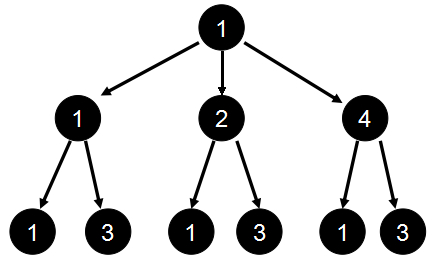
\includegraphics[height = 5cm,width = 9cm]{anti_prime.jpg}\\
这棵树除了第一层外,每一层对应着一个素数,从上到下递增;每一层的每一个节点对应着素数的幂,从左到右递增,每一条从根节点到叶节点的路径上数字相乘即为一个约数。 我们要想获得 $g(n)=x $的最小正整数,就要求$n$的质因子尽可能小,且尽可能多,换而言之就是幂次尽可能为$1$,所以就要对上面的树进行从上到下从左到右的$dfs$直到约数个数满足 $x$ 。 \\

\underline {【Codeforces 27E】给定一个数$n$,求一个最小的正整数,使得的约数个数为$n$.}

\begin{lstlisting}
typedef unsigned long long lint;
const lint inf = ~0ull;
const int prime[]= {2, 3, 5, 7, 11, 13, 17, 19, 23, 29, 31, 37, 41, 43, 47, 53};

int n;
lint ans;

void dfs(int depth, int limit, lint tmp, int num)
{
	if(num > n) return;
	if(num == n && tmp < ans) ans = tmp;
	for(int i = 1; i <= limit; ++i) { // i 相当于幂次
		if((double)tmp * prime[depth] > ans) break; // 不用扩展树的深度
		tmp *= prime[depth];
		if(n % (num * (i + 1)) == 0) {
			dfs(depth + 1, i, tmp, num * (i + 1));
		}
	}
}

int main()
{
	while(cin >> n){
		ans = inf;
		dfs(0, 63, 1, 1);
		cout << ans << endl;
	}
	return 0;
}
\end{lstlisting}

\underline {【URAL 1748】:给定一个数$n$,求$[1,n]$内约数个数最多的且数值最小的数,以及其约数个数$(n\leq 10^{18})$。}

\begin{lstlisting}
//将搜索改为当前值 tmp > n 时终止,初始化ans = inf, cnt = 0
//主函数里调用 dfs(0, 63, 1, 1) ,初始化 prime[] 同例1
void dfs(int depth, int limit, lint tmp, int num)
{
	if(tmp > n) return;
	if(num > cnt || (num == cnt && tmp < ans)) {
		ans = tmp;
		cnt = num;
	}
	for(int i = 1; i <= limit; ++i) {
		if((double)tmp * prime[depth] > n) break;
        //需要用 double 强制类型转换,否则爆数据
		tmp *= prime[depth];
		dfs(depth + 1, i, tmp, num * (i + 1));

	}
}
\end{lstlisting}

\section{卢卡斯定理}

用于解决组合数取模问题$C_{n}^{m}\ \% p\ \ (m\leq n \leq 10^{18},p$为素数) \\

当$1\leq m \leq n \leq 10^{18},2\leq p \leq 10^5$且$p$是素数时,如果: \\
$$n=n_kp^k+n_{k-1}p^{k-1}+...+n_1p+n_0$$
$$m=m_kp^k+m_{k-1}p^{k-1}+...+m_1p+m_0$$
那么: \\
$$C_{n}^{m}\ \% p=\prod_{i=0}^{k}C_{n_i}^{m_i}\ (mod \ p)$$
\begin{lstlisting}
inline ll C(ll a, ll b)
{ //计算组合数 C[a][b] ,如果是小数据并且模数固定可以预处理阶乘
	if(b > a) return 0;
	ll res = 1, x, y;
	for(int i = 1; i <= b; ++i) {
		x = (a + i - b) % mod;
		y = i % mod;
		res = res * x % mod * quick_pow(y, mod - 2) % mod; //模素数逆元
	}
	return res;
}
inline ll Lucas(ll n, ll m)
{
	if (n < 0 || m < 0 || m > n) return 0;
	if (m == 0) return 1;
	return C(n % mod, m % mod) * Lucas(n / mod, m / mod) % mod;
}
\end{lstlisting}

\subsection{给定$n$求$C_{n}^{m}(0\leq m\leq n\leq 10^8)$为奇数的$m$个数}

\underline {[HDU 4349]}

即$C_{n}^{m}\ \%2=1$的$m$个数,考虑将$n$和$m$都表示成$2$的幂次组合形式,则任意的系数$n_i$和$m_i$非0即1.因为$C_0^0=C_1^0=C_1^1=1$,所以根据$Lucas$定理,如果$n_i=0$,则$m_i=0$,如果$n_i=1$,则$m_i=0$或$1$,根据乘法原理每个$n_i=1$,对于$m_i$ 都有$2$种选择,那么$ans=2^{cnt}$,其中$cnt$ 是$n$分解为$2$的幂次形式系数为$1$的项个数

\begin{lstlisting}
scanf("%d", &n);
cnt = 0;
while (n) {
	if (n & 1) cnt ++;
	n >>= 1;
}
printf("%d\n", 1 << cnt);
\end{lstlisting}

\clearpage
\section{特殊方法}

\subsection{$n^k$的高三位}

对于给定的一个数$n$,它可以写成$10^a$,其中$a$为浮点数,则$n^k=(10^a)^k=10^{a*k}=10^x*10^y$;其中$x,y$分别是$a*k$的整数部分和小数部分.对于$t=n^k$这个数,它的位数由$10^x$决定,它的位数上的值则有$10^y$决定,因此我们要求$t$的前三位,只需要将$10^y$求出,在乘以$100$,就得到了它的前三位。$fmod(x,1)$可以求出$x$的小数部分。(或者使用$floor$函数)

\begin{lstlisting}
high_three_digits = (int)pow(10.0, 2.0 + fmod(k * 1.0 * log10(n * 1.0), 1)).
或者double t = 1.0 * k * log10(n * 1.0);
high_three_digits = (int)(pow(10.0, t - (int)floor(t) + 2.0));
\end{lstlisting}

\subsection{约数个数之和,定义$d(i)$为$i$的约数个数}

$$\sum_{i=1}^{a}d(i)=\sum_{}\lfloor {\frac{a}{i}}\rfloor$$
$$\sum_{i=1}^{a}\sum_{j=1}^{b}d(i*j)=\sum_{gcd(i,j)=1}\lfloor{\frac{a}{i}}\rfloor \lfloor{\frac{b}{j}}\rfloor$$
$$\sum_{i=1}^{a}\sum_{j=1}^{b}\sum_{k=1}^{c}d(i*j*k)=\sum_{gcd(i,j)=gcd(j,k)=gcd(i,k)=1}\lfloor{\frac{a}{i}}\rfloor \lfloor{\frac{b}{j}}\lfloor {\frac{c}{k}}\rfloor$$
这个性质可以推广到$n$维 \\

\underline {[BZOJ 3994]:求$\sum_{i=1}^{n}\sum_{j=1}^{m}d(i*j)$,定义$d(i)$为$i$的约数个数.$n,m\in [1, 50000]$}

$$\begin{aligned}
ans &=\sum_{gcd(i,j)=1}\lfloor{\frac{n}{i}}\rfloor \lfloor{\frac{m}{j}}\rfloor
&= \sum_{i=1}^{n}\lfloor{\frac{n}{i}}\rfloor\sum_{j=1}^{m} \lfloor{\frac{m}{j}}\rfloor
\end{aligned}$$

$定义g(n)=\sum_{i=1}^{n}\lfloor{\frac{n}{i}}\rfloor=\sum_{i= 1}^{n}d(i)$,只需要预处理出$g(n)$就可以在$O(\sqrt n)$时间范围内解决问题。如果选择分步加速的话,预处理的复杂度是$O(n\sqrt n)$,但是其实我们考虑每个数$i$的约数个数,然后$g(n)$就是前缀和了。\\
在线性筛时每个合数是被最小质因子筛掉的,我们只需要记录这个每个数$m$最小质因子的幂次$num[m],d[m]$记录$m$的约数个数,显然$d(m)$ 是积性函数.对于$m=i*prime[j]$,如果$i\ \% \  prime[j]!=0$,根据积性函数性质$num[m]=1,d[m]=d[i]*d[prime[j]],$否则$num[m]=num[i]+1,$ 因为$m$的约数个数是:$(e_1+1)*(e_2+1)*...*(e_k+1),e_i$ 是质因子分解后各质因子的幂次,我们考虑$m$从$i$的转移过程,$m$只比$i$在$prime[j]$的幂次上多$1$,所以$d[m]=\frac{d[i]}{num[i]+1]}*(num[i]+2)$.
\begin{lstlisting}
void GetMu()//线性时间预处理
{
	bs.set();
	prime_cnt = 0;
	mu[1] = d[1] = 1;
	for(int i = 2; i < MAX_N; ++i) {
		if(bs[i]) {
			prime[prime_cnt++] = i;
			mu[i] = -1;
			num[i] = 1;
			d[i] = 2;
		}
		for(int j = 0; j < prime_cnt && i * prime[j]  < MAX_N; ++j) {
			bs[i * prime[j]] = 0;
			if(i % prime[j]) {
				mu[i * prime[j]] = -mu[i];
				num[i * prime[j]] = 1;
				d[i * prime[j]] = d[i] * d[prime[j]];
			}else {
				mu[i * prime[j]] = 0;
				num[i * prime[j]] = num[i] + 1;
				d[i * prime[j]] = d[i] / (num[i] + 1) * (num[i] + 2);
				break;
			}
		}
	}
	for(int i = 1; i < MAX_N; ++i) {
		sum[i] = sum[i - 1] + mu[i];
		g[i] = g[i - 1] + d[i];
	}
}
void Get_g() // O(n * sqrt(n)) 的预处理
{
	int last;
	for(int n = 1; n < MAX_N; ++n) {
		for(int i = 1; i <= n; i = last + 1) {
			last = n / (n / i);
			g[n] += (ll) (last - i + 1) * (n / i);
		}
	}
}

inline ll solve(int n, int m)
{
	ll res = 0;
	int top = min(n, m), last;
	for(int i = 1; i <= top; i = last + 1) {
		last = min(n / (n / i), m / (m / i));
		res += (sum[last] - sum[i - 1]) * g[n / i] * g[m / i];
	}
	return res;
}
\end{lstlisting}

对于【Codeforces 235 E Number Challenge】:
$$\sum_{i=1}^{a}\sum_{j=1}^{b}\sum_{k=1}^{c}d(ijk),a,b,c\in [1,2000]$$
利用上述结论反演可得:
$$Ans =\sum_{i=1}^{i=a}{\lfloor{\frac{a}{i}}}\rfloor\sum_{d}^{min(b,c)}μ(d)\sum_{d|j,(i,j)=1}\lfloor{\frac{b}{j}}\rfloor\sum_{d|k,(i,k)=1}\lfloor{\frac{c}{k}}\rfloor$$
记$j=dj',k=dk'$,则:
$$Ans=\sum_{i=1}^{i=a}{\lfloor{\frac{a}{i}}}\rfloor\sum_{d}^{min(b,c)}μ(d)\sum_{gcd(i,dj')=1}\lfloor{\frac{b}{dj'}}\rfloor\sum_{gcd(i,dk')=1}\lfloor{\frac{c}{dk'}}\rfloor$$
因为$gcd(i,dj')=1$,我们先保证$gcd(i,d)=1,$然后枚举$j':1 \rightarrow \frac{b}{d}$,保证$gcd(i,j')=1$,这样就可以使得$gcd(i,dj')=1$,累加即可。对于$gcd(i,dk')=1$同样处理。时间复杂度是:$O(a*b*log(b))$

\begin{lstlisting}
//需要预处理 GetMu() 和 GetGcd()
inline ll work(int n, int x)
{
	ll res = 0;
	for(int i = 1; i <= n; ++i) {
		if(gcd[i][x] == 1) {
			res = (res + (n / i)) % mod;
		}
	}
	return res;
}

inline ll solve(int a, int b, int c)
{
	ll res = 0;
	int top = min(b, c);
	for(int i = 1; i <= a; ++i) {
		for(int d = 1; d <= top; ++d){
			if(gcd[i][d] == 1) {
				ll tmp = 0;
				tmp = (ll) (a / i) * mu[d] * work(b / d, i)
                            % mod * work(c / d, i) % mod;
				res = ((res + tmp) % mod + mod) % mod;
			}
		}
	}
	return res;
}
\end{lstlisting}

\subsection{给定$k$,求最小的$n$使得$n$的约数个数恰为$n-k$个$(k\leq 47777)$}
\underline {【HDU 4542】}

\begin{lstlisting}
const int MAX_N = 50010;
int id[MAX_N];
void init()
{
	for(int i = 1; i < MAX_N; ++i) id[i] = i;
// 初始化 id[i] 最多有 i 个数与其互质
	for(int i = 1; i < MAX_N; ++i) {
		for(int j = i; j < MAX_N; j += i) id[j]--;
//根据 j 的约数有 i,id[j]--
		if(id[id[i]] == 0) id[id[i]] = i;
		// 因为我们最终是要将 id[k] 表示成约数个数为 n-k 的最小数 n ,
        // 如果此时 id[id[i]]=0 说明小于 i 的数中不存在数 x , 使得 x 的约数个数为 x-id[i]
        // 那么实际上使得约数个数恰为 n-id[i] 的最小数 n 只能是 i 了
		id[i] = 0;
// 显然小于等于 i 的数不存在数 x 使得 x 的约数个数恰为 x-i 个,所以要赋 id[i]=0
	}
} // 对于 id[i] 等于 0 的 i ,实际上就不存在数 x 使得 x 的约数个数恰为 x-i 个
\end{lstlisting}

\subsection{$C_{n}^{m}\mod \ p(p=p_1*p_2$,且$p_1,p_2$为素数)}

我们把$C_{n}^{m}\ \ \% \ \ p$的值记为$x$,把$C_{n}^{m}\ \%\  p_1$的值记为$x1$,把$C_{n}^{m}\ \%\  p_2$的值记为$x2$,则有: \\
$$x \equiv \ x_1(\% \ \ p_1)\qquad x \equiv \ x_2(\% \ \ p_2)$$
因为$p_1,p_2$都是素数,所以$x_1$和$x_2$都可以用$Lucas$定理求解出来。利用中国剩余定理求解同余方程。\\
定义:
\begin{center}
$inv_1$为:($p_2$在模$p_1$域下的逆元)$*p_2$\\
$inv_2$为:($p_1$在模$p_2$域下的逆元)$*p_1$
\end{center}

\begin{lstlisting}
//quick_pow( a, b, c): (a ^ b) % c
inv1 = quick_pow(p2, p1 - 2, p1) * p2;
inv2 = quick_pow(p1, p2 - 2, p2) * p1;
\end{lstlisting}
那么答案就是:\\
$$x=(inv_1*x_1\ + inv_2 * x_2)\% \ p$$

%\end{document}

%\documentclass[UTF8]{book} % 使用book文档类型格式排版
\usepackage{ctex}  %加载包,因为我们在用中文写文档,所以必须加载这个包,否则不支持中文

%加入了一些针对XeTeX的改进并且加入了 \XeTeX 命令来输入漂亮的XeTeX logo
\usepackage{xltxtra}
%启用一些LaTeX中的功能
\usepackage{xunicode}

\usepackage{multicol}  %加载包
\usepackage{amsmath} % 调用公式宏包
\usepackage{amssymb} % 数学符号生成命令
\usepackage{array} % 数组和表格制作
\usepackage{booktabs} % 绘制水平表格线
\usepackage{calc} %四则运算
\usepackage{caption} % 插图和表格标题格式设置
\usepackage{fancyhdr} % 页眉页脚设置
\usepackage{graphicx} % 调用插图宏包
\usepackage{multicol} % 多栏排版
\usepackage{titlesec} % 章节标题格式设置

%%%% 目录样式 %%%%
\usepackage{titletoc}
\titlecontents{chapter}[1pt]{\vspace{.5\baselineskip}\bfseries}
    {{\thecontentslabel}\quad}{}
    {\hspace{.5em}\titlerule*[10pt]{$\cdot$}\contentspage}
\titlecontents{section}[2em]{\vspace{.25\baselineskip}\bfseries}
    {\thecontentslabel\quad}{}
    {\hspace{.5em}\titlerule*[10pt]{$\cdot$}\contentspage}

\usepackage{color}
\usepackage{xcolor} % 颜色处理
%\usepackage{indentfirst} % 自动首行缩进
%\setlength{\parindent}{2.22em} % 设置首行缩进的距离
% 设置超链接颜色
\usepackage[colorlinks=true,linkcolor=black,urlcolor=black,citecolor=black]{hyperref} % 根据章节标题生成PDF书签

%%%% 版面 %%%%
\usepackage[top=0.5in,bottom=0.5in,left=1.25in,right=0.8in]{geometry}
% 设置行距
\linespread{1}
\usepackage{lscape}
\usepackage{listings} %插入代码,代码页需要加入[fragile]
\usepackage{xeCJK}

%\usepackage[slantfont,boldfont]{xeCJK} % 允许斜体和粗体

%%%% fontspec 宏包 %%%%
\usepackage{fontspec}
% 指定字体
%\setmonofont[Mapping={}]{Monaco}	%英文引号之类的正常显示,相当于设置英文字体
%\setsansfont{Monaco} %设置英文字体 Monaco, Consolas,  Fantasque Sans Mono
%\setmainfont{Monaco} %设置英文字体
% \setCJKmainfont{方正兰亭黑简体}  %中文字体设置
% \setCJKsansfont{华康少女字体} %设置中文字体
% \setCJKmonofont{华康少女字体} %设置中文字体

%%%%%%%%%% 图形支持宏包 %%%%%%%%%%
\usepackage{graphicx}                % 嵌入png图像
\usepackage{color,xcolor}            % 支持彩色文本、底色、文本框等
%\usepackage{subfigure}
%\usepackage{epsfig}                 % 支持eps图像
%\usepackage{picinpar}               % 图表和文字混排宏包
%\usepackage[verbose]{wrapfig}       % 图表和文字混排宏包
%\usepackage{eso-pic}                % 向文档的部分页加n副图形, 可实现水印效果
%\usepackage{eepic}                  % 扩展的绘图支持
%\usepackage{curves}                 % 绘制复杂曲线
%\usepackage{texdraw}                % 增强的绘图工具
%\usepackage{treedoc}                % 树形图绘制
%\usepackage{pictex}                 % 可以画任意的图形
%\usepackage{hyperref}

%\setCJKmainfont{Kai}   % 设置缺省中文字体
%\setCJKmonofont{Hei}   % 设置等宽字体
%\setmainfont{Optima}   % 英文衬线字体
%\setmonofont{Monaco}   % 英文等宽字体
%\setsansfont{Trebuchet MS} % 英文无衬线字体

\makeatletter
\providecommand*\input@path{}
\newcommand\addinputpath[1]{
\expandafter\def\expandafter\input@path
\expandafter{\input@path{#1}}}
\addinputpath{body/}
\makeatother

\definecolor{keywordcolor}{rgb}{0.8,0.1,0.5}
\lstset{language=C++, %用于设置语言为C++
    numbers=left, %设置行号位置
    numberstyle=\tiny, %设置行号大小
    keywordstyle=\color{keywordcolor} \bfseries,
    identifierstyle=,
    basicstyle=\ttfamily,
    commentstyle=\color{blue} \textit, %注释颜色
    stringstyle=\ttfamily,
    showstringspaces=false,
    frame=shadowbox, %边框
    %frame = single,
    tabsize=2, %设置tab空格数
    showspaces=false, %不显示空格
    escapeinside=``, %逃逸字符(1左面的键),用于显示中文
    %breaklines, %自动折行
    captionpos=b
}
%\begin{document}

\chapter{数学相关}

\section{Polya原理、Burnside引理}

\subsection{介绍}
群:\\
给定一个集合$G=\{a,b,c,...\}$和集合$G$上的二元运算$\star$,并满足\\
\begin{itemize}
\item 封闭性:$\forall a,b\in G,\exists c \in G,a \star b = c.$
\item 结合律:$\forall a,b,c \in G,(a \star b) \star c= a \star (b \star c).$
\item 单位元:$\exists e \in G,\forall a \in G, a \star e = e \star a = a.$
\item 逆元:$\forall a \in G,\exists b \in G, a \star b = b \star a = e,记b=a^{-1}$
\end{itemize}

则称集合$G$在运算$\star$之下是一个群,简称$G$是群。一般$a\star b$简写为$ab$。\\
置换:\\
$n$个元素$1,2,...,n$之间的置换$\begin{pmatrix} 1 & 2 & ... & n \\ a_1 & a_2  & ... & a_n\end{pmatrix}$,表示$1$被$1$到$n$中的某个数$a_1$取代,$2$被$1$到$n$中的某个数$a_2$取代,直到$n$被$1$到$n$中的某个数$a_n$取代,且$a_1,a_2,…,a_n$互不相同 \\
置换群:\\
置换群的元素是置换,运算是置换的连接。例如: \\
$\begin{pmatrix} 1& 2 & 3 & 4 \\ 3 & 1  & 2 & 4\end{pmatrix}$ $\begin{pmatrix} 1& 2 & 3 & 4 \\ 4 & 3  & 2 & 1\end{pmatrix}$ = $\begin{pmatrix} 1& 2 & 3 & 4 \\ 3 & 1  & 2 & 4\end{pmatrix}$$\begin{pmatrix} 3& 1 & 2 & 4 \\ 2 & 4  & 3 & 1\end{pmatrix}$=$\begin{pmatrix} 1& 2 & 3 & 4 \\ 2 & 4  & 3 & 1\end{pmatrix}$ \\
$Z_k $($K$不动置换类):\\
设$G$是$1…n$的置换群。若$K$是$1…n$中某个元素,$G$中使$K$保持不变的置换的全体,记以$Z_k$,叫做$G$中使$K$保持不动的置换类,简称$K$不动置换类。 \\
$E_k$(等价类):\\
设$G$是$1…n$的置换群。若$K$是$1…n$中某个元素,$K$在$G$作用下的轨迹,记作$E_k$。即$K$在$G$的作用下所能变化成的所有元素的集合。 \\
$$\mid E_k\mid· \mid Z_k\mid=\mid G\mid   \ \ \  k=1…n$$
$ D(a_j)$ 表示在置换$a_j$下不变的元素的个数 ,$s$表示置换种类数: \\
$$\sum_{i=1}^{n}\mid Z_i \mid = \sum_{i=1}^{s}D(a_i)$$

\subsection{$Burnside$引理}
 $\ L= \frac{1}{\mid G \mid}\sum_{i=1}^{n}\mid Z_i \mid = \frac{1}{\mid G \mid}\sum_{i=1}^{s}D(a_i)$,$ \ \ L$ 就是等价类数,也就是互异的组合状态的个数。\\
证明:不妨设$N={1,……,n}$中共有$L$个等价类,$N=E^1+ E^2+……+E^L$,则当$j$和$k$属于同一等价类时,有$\mid Z_j \mid = \mid Z_k \mid$。 所以\\
$$\sum_{i=1}^{n}\mid Z_i \mid = \sum_{i=1}^{L} \sum_{k \in E_i} \mid Z_k \mid = \sum_{i=1}^{L}\mid E_i \mid \cdot \mid Z_i \mid =L \cdot \mid G \mid $$

循环:\\
记$(a_1a_2...a_n)$=$\begin{pmatrix} a_1& a_2 & ... & a_{n-1} & a_n \\ a_2 & a_3   & ... & a_n & a_1 \end{pmatrix}$ 称为 $n$阶循环。每个置换都可以写成若干互不相交的循环的乘积,两个循环$(a_1a_2...a_n)$和$(b_1b_2...b_n)$互不相交是指$a_i \neq b_j,i,j=1,2,...,n$.,\\
例如:$\begin{pmatrix} 1& 2 & 3 & 4  & 5\\ 3 & 5 &  1  & 4 & 2\end{pmatrix}$ =$(1 \ 3)(2 \ 5)(4)$.这样的表示是唯一的。置换的循环节数是上述表示中循环的个数。例如$(1 \ 3)(2 \ 5)(4)$的循环节数是$3$。特别的:当$n=2$时,两阶循环$(i,j)$叫做$i$和$j$的对换。任何一个循环,都可以表达成若干换位之积。但是表达形式不尽统一,甚至连换位个数都不相同。\\
例如$(123)=(12) (13) =(13) (23) =(21)(23)=(12)(13)(31)(13)$。 尽管如此,有一个性质却是固有的,它不依换位的个数不同而异,那就是循环分解成换位的乘积时,换位个数奇偶性是不变的,或分解成奇数个换位之积或分解成偶数个换位之积。\\
若一个置换分解成奇数个换位之积,叫做奇置换;若分解成偶数个换位之积叫偶置换。单位置换为偶置换。\\

\subsection{Polya原理}

设$G$是$p$个对象的一个置换群,用$m$种颜色涂染$p$个对象,$G=\{g_1,g_2,...,g_s\}$,$g_i$是不同的置换选择,令$g_i$的循环节数为$c(g_i)\ (i \ \in [1,s])$,则不同的染色方案数为:$L \ = \frac{1}{\mid  G \mid}(m^{c(g_1)}\ + m^{c(g_2)}\ +... + m^{c(g_s)})$ \\

\subsection{$n*n$的方阵,每个小格可涂$m$种颜色,求在旋转操作下本质不同的解的总数}

我们可以在方阵中分出互不重叠的长为$[\frac{n+1}{2}]$,宽为$[\frac{n}{2}]$的四个矩阵。当$n$为偶数时,恰好分完;当$n$为奇数时,剩下中心的一个格子,它在所有的旋转下都不动,所以它涂任何颜色都对其它格子没有影响。令$m$种颜色为$0\sim m-1$,我们把矩阵中的每格的颜色所代表的数字顺次(左上角从左到右,从上到下;右上角从上到下,从右到左;……)排成$m$进制数,然后就可以表示为一个十进制数,其取值范围为 $0 \sim m^{\frac{n^2}{4}}-1$。(因为$\frac{n}{2}*\frac{n+1}{2}=\frac{n^2}{4}$) 这样,我们就把一个方阵简化为$4$个整数。我们只要找到每一个等价类中左上角的数最大的那个方案(如果左上角相同,就顺时针方向顺次比较) 这样,在枚举的时候其它三个数一定不大于左上角的数,效率应该是最高的。  进一步考虑,当左上角数为$i$时,($i \in [0, R-1]$). 令$R=m^{\frac{n^2}{4}}$ 可分为下列的4类:
\begin{enumerate}
\item  其它三个整数均小于$i$,共$i^3$个。
\item 右上角为$i$,其它两个整数均小于$i$,共$i^2$个。
\item  右上角、右下角为$i$,左下角不大于$i$,共$i+1$个。
\item  右下角为$i$,其它两个整数均小于$i$,且右上角的数不小于左下角的,共$\frac{i\ *\ (i+1)}{2}$个。
\end{enumerate}

因此:
\[
\begin{aligned}
L&=\sum_{i=0}^{R-1}(i^3+i^2+i+1+\frac{1}{2}i(i+1))=\sum_{i=0}^{R-1}(i^3+\frac{3}{2}i^2+\frac{3}{2}i+1) \\
&=\sum_{i=1}^{R}((i-1)^3+\frac{3}{2}(i-1)^2+\frac{3}{2}(i-1)+1)=\sum_{i=1}^{R}(i^3-\frac{3}{2}i^2+\frac{3}{2}i) \\
&=\frac{1}{4}R^2(R+1)^2-\frac{3}{2}*\frac{1}{6}R(R+1)(2R+1)+\frac{3}{2}*\frac{1}{2}R(R+1) \\
&=\frac{1}{4}(R^4+R^2+2R) \\
\end{aligned}
\]

当$n$为奇数时,还要乘以一个$m$. \\

\underline {采用$Polya$原理解决} \\
确定置换群: \\
只有$4$个置换:$转0^\circ ,转90^\circ,转180^\circ,转270^\circ$,所以置换群$G=\{转0^\circ ,转90^\circ,转180^\circ,转270^\circ\}$ \\
计算循环节个数: \\
首先,给每个格子顺次编号$(1\sim n^2)$,再开一个二维数组记录置换后的状态。最后通过搜索计算每个置换下的循环节个数,效率为一次方级。\\
代入公式 : \\
利用$Pólya$定理得到最后结果。\\
$$L \ = \frac{1}{\mid  G \mid}(m^{c(g_1)}\ + m^{c(g_2)}\ +... + m^{c(g_s)})$$
当然也可以直接思考循环节: \\
\begin{itemize}
\item 当$n$为偶数,在转$0^\circ$时,循环节为$n^2$个,转$180^\circ$时,循环节为$\frac{n^2}{2}$个,转$90^\circ$和$270^\circ$时,循环节为$\frac{n^2}{4}$ 个
\item 当$n$为奇数,在转$0^\circ$时,循环节为$n^2$个,转$180^\circ$时,循环节为$\frac{n^2 - 1}{2} + 1$个,转$90^\circ$和$270^\circ$时,循环节为$\frac{n^2 - 1}{4}+1$个
\end{itemize}
综合考虑可得:$L \ = \frac{1}{4}(m^{n^2} + m^{\frac{n^2+3}{4}}\ +m^{\frac{n^2+1}{2}} + m^{\frac{n^2+3}{4}})$。可以发现这个式子,其实是和数学推导的式子完全吻合的。
\begin{lstlisting}
typedef long long ll;
const int MAX_N = 10;
const ll mod = 1000000007;

int a[MAX_N][MAX_N], b[MAX_N][MAX_N];
int m, n; // m: 颜色数, n: 方阵大小
ll ans;

void Rotate() //逆时针旋转 90 度
{
	for(int i = 1; i <= n; ++i) {
		for(int j = 1; j <= n; ++j) {
			a[n - j + 1][i] = b[i][j];
		}
	}
	for(int i = 1; i <= n; ++i) {
		for(int j = 1; j <= n; ++j) {
			b[i][j] = a[i][j];
		}
	}
}

void CircleSection() //计算当前状态循环节数
{
	int num = 0; //记录循环节个数
	for(int i = 1; i <= n; ++i) {
		for(int j = 1; j <= n; ++j) {
			if(a[i][j] > 0) { //搜索尚未被访问过的格子
				num++;
				int nexti, nextj, p;
				p = a[i][j];
				a[i][j] = 0;
				nexti = (p - 1) / n + 1;
				nextj = (p - 1) % n + 1; //得到这个循环的下一个格子
				while(a[nexti][nextj] > 0) {
					p = a[nexti][nextj];
					a[nexti][nextj] = 0; //已访问格子置零
					nexti = (p - 1) / n + 1;
					nextj = (p - 1) % n + 1;
				}
 			}
		}
	}
	ll res = 1;
	for(int i = 1; i <= num; ++i ) {
		res = res * m % mod;
	}
	ans = (ans + res) % mod;
}

void init()
{
	for(int i = 1; i <= n; ++i) {
		for(int j = 1; j <= n; ++j) {
			b[i][j] = a[i][j] = (i - 1) * n + j;
		}
	}
}

int main()
{
	ll tt = quick_pow(4, mod - 2); //求除以 4 模 mod 的逆元
	while(~scanf("%d%d", &n, &m)){
		ans = 0;
		init(); //对方阵状态进行初始化
		CircleSection(); //旋转 0 度状态下的循环节个数
		Rotate();
		CircleSection();//逆时针 90 度
		Rotate();
		CircleSection(); //逆时针 180 度
		Rotate();
		CircleSection();//逆时针 270 度
		Rotate();
		ans = ans * tt % mod;
		printf("ans = %lld\n", ans); //根据 Polya 原理得到的结果

		ll R = quick_pow(m, n * n / 4);
		ll res = R * R % mod * R % mod * R % mod + R * R % mod + 2 * R % mod ;
		if(n & 1) res = res * m % mod;
		res = res * tt % mod;
		printf("res = %lld\n", res); //根据数学推导得到的结果
	}
	return 0;
}
\end{lstlisting}

\subsection{各有$a,b,c(a,b,c \geq  0, a+b+c \leq 40)$颗三种颜色,问这些珠子能串成的项链有多少种?考虑翻转和旋转。}
\underline {[UVA 11255 Necklace]} \\
令$\sum_{i=1}^{3}color[i]=n$,即珠子总数。 \\

考虑旋转置换 \\

我们考虑旋转$i$颗珠子的间距,则$0,i,2i...$构成一个循环,这个循环有$\frac{n}{gcd(n,i)}$.根据对成性,所有循环的长度均相同,因此一共有$gcd(i,n)$个循环。循环与循环之间是等价类,所以在一个循环内的某颗珠子的颜色确定了,那么在其余循环内的同样地位位置的珠子颜色也就确定了。我们得到的答案是每个循环的方案数并且在旋转置换下,当循环节确定了,每个循环的方案数都是一样的 。我们假设循环节的长度(也就是循环内元素的个数)为$x\in [0,n)$,第$i$种颜色的珠子的个数为$color[i]$个,如果$color[i] \% x !=0$,那么第$i$种颜色的珠子在每个循环(等价类)内就不能均分,所以这种循环节就应该摒弃。当$color[i] \% x ==0$时,令$b[i] = \frac{color[i]}{x}$,则$b[i]$就是每个循环(等价类)分得的这种颜色的珠子的个数。显然每个循环(等价类)内共有$\sum_{i=1}^{3}b[i]=\frac{1}{x}\sum_{i=1}^{3}color[i]$颗珠子,记为$sum$. 我们考虑单个循环(等价类):有$sum$颗珠子,各个颜色分别有$b[i]$颗,那么根据排列组合在循环节为$x$时,可得$$Ans[x]=C_{sum}^{b[0]}*C_{sum-b[0]}^{b[1]}*C_{sum-b[0]-b[1]}^{b[2]}$$

考虑翻转置换 \\

当$n$为奇数时,则对称轴上必有一点,对称轴有$n$条,每条对称轴形成$\frac{n-1}{2}$个长度为$2$的循环和$1$个长度为$1$的循环。\\

当$n$为偶数时,有两种对称轴。穿过珠子的对称轴有$\frac{n}{2}$条,各形成$\frac{n}{2}-1$个长度为2的循环和两个长度为$1$的循环。不穿过珠子的对称轴也有$\frac{n}{2}$条,各形成$\frac{n}{2}$个长度$2$的循环。\\

可以发现不论$n$为奇偶,对称轴的总个数都为$n$,同时旋转置换的个数也为$n$,所以根据$Burnside$引理最后需要除以$2n$.

\begin{lstlisting}
const int MAX_N = 42;

ll C[MAX_N][MAX_N];
int color[5], b[5], n;

void init() //组合数打表
{
	C[0][0] = 1;
	for(int i = 1; i < MAX_N; ++i) {
		C[i][0] = C[i][i] = 1;
		for(int j = 1; j < i; ++j) {
			C[i][j] = C[i - 1][j] + C[i - 1][j - 1];
		}
	}
}

int gcd(int x, int y)
{
	return y == 0 ? x : gcd(y, x % y);
}

ll CircleSection(int x)
{
	int sum = 0;
	for(int i = 1; i <= 3; ++i) {
		if(b[i] % x) return 0;
		b[i] /= x;
		sum += b[i];
	}
	ll res = 1;
	for(int i = 1; i <= 3; ++i) {
		res *= C[sum][b[i]];
		sum -= b[i];
	}
	return res;
}

ll Rotate() //旋转置换
{
	ll res = 0;
	for(int i = 0; i < n; ++i) {
		int d = gcd(i, n);
		memcpy(b, color, sizeof(color));
		res += CircleSection(n / d); // n/d 是循环元素个数
	}
	return res;
}

ll Flip() //翻转置换
{
	ll res = 0;
	if(n & 1) {
		for(int i = 1; i <= 3; ++i) {
			memcpy(b, color, sizeof(color));
			b[i]--;
			if(b[i] < 0) continue;
			res += CircleSection(2) * n; // n 条对称轴
		}
	}else {
		//穿过珠子
		for(int i = 1; i <= 3; ++i) {
			for(int j = 1; j <= 3; ++j) {
				memcpy(b, color, sizeof(color));
				b[i]--, b[j]--;
				if(b[i] < 0 || b[j] < 0) continue;
				res += CircleSection(2) * (n / 2);
			}
		}
		//不穿过珠子
		memcpy(b, color, sizeof(color));
		res += CircleSection(2) * (n / 2);
	}
	return res;
}

int main()
{
	init();
	int T;
	scanf("%d", &T);
	while(T--) {
		n = 0;
		for(int i = 1; i <= 3; ++i) {
			scanf("%d", color + i);
			n += color[i];
		}
		ll ans = 0;
		ans += Rotate();
		ans += Flip();
		printf("%lld\n", ans / (2 * n));
	}
	return 0;
}
\end{lstlisting}

\subsection{给出12根等长的火柴棒,每根火柴棒的颜色属于$1-6$中的一种,问能拼成多少种不同的正方体?(考虑旋转)}

\underline {[UVA 10601 Cubes]}首先正方体的旋转置换有$24$种。下面将每个循环内元素的个数称为循环的长度。\\

\underline{注意是棱边的置换循环,而不是面的置换循环}.\\
\begin{enumerate}
\item 静止。只有一种置换。有$12$个循环,每个循环的长度为$1$。
\item 以相对面的中心为轴旋转。可以旋转的角度是$90^{\circ},180^{\circ},270^{\circ}$。 选择轴有3种,每种轴下有3种旋转,所以有3*3=9 种置换。
\item 旋转$90^{\circ},270^{\circ}$ ,都是三个循环,每个循环的长度为$4$.
\item 旋转$180^{\circ}$,有6个循环,每个循环的长度为2
\item 以对边中点为轴,只可以旋转$180^{\circ}$,选择轴有6种,所以有6*1=6种置换。在这种旋转下有5个长度为2的循环和2个长度为1的循环
\item 以对顶点为为轴,可以旋转$120^{\circ},240^{\circ}$。 选择轴有4种,所以有4*2=8种置换。
\item 旋转$120^{\circ},240^{\circ}$都是有4个长度为3的循环。
\end{enumerate}
找到了在每种置换下的循环个数和每个循环的长度就可以参考前面【例2】处理旋转置换的方法解决。 \\
需要特别关注的是,\underline {以对边中点为轴,只可以旋转$180^{\circ}$,有5个长度为2的循环和2个长度为1的循环。} \\
我们可以先枚举两个长度为1的循环选择的颜色,然后对于5个长度为2的循环就和上面的一样了。最后别忘了根据$Burnside$引理需要除以总的置换数$24$。

\begin{lstlisting}
ll work(int k)
{ //每 k 条边必须相同,分成 12/k 组(以对边中点为轴旋转 180° 是分成 5 组)
	memcpy (b, a, sizeof(a));
	int sum = 0;
	for (int i = 1; i <= 6; ++i) {
		if(b[i] % k) return 0;
		b[i] /= k;
		sum += b[i];
	}
	ll res = 1;
	for (int i = 1; i <= 6; ++i) {
		res *= C[sum][b[i]];
		sum -= b[i];
	}
	return res;
}

ll solve()
{
	ll res = 0;
	//静止
	res += work(1);
	//以相对面中心为轴
	res += (ll)3 * 2 * work(4); //旋转 90° 和270°
	res += (ll)3 * work(2); //旋转180°
	// 以对顶点为轴,可以旋转 120° 或 240°
	res += (ll)4 * 2 * work(3);
	// 以对边种点为轴,只能旋转 180°
	for(int i = 1; i <= 6; ++i) {
		for(int j = 1; j <= 6; ++j) {
			if(a[i] == 0 || a[j] == 0) continue;
			a[i]--; a[j]--;  // 将 a[i] 和 a[j] 设为选择的两条对边的颜色
			res += (ll)6 * work(2);
        //剩下的是 5 个循环长度为 2 的循环, 6 代表对边选择情况
			a[i]++; a[j]++;
		}
	}
	return res / 24;
}
\end{lstlisting}

\subsection {[POJ 2888 Magic Bracelet]}

有一串$n$个珠子的项链,用$m$种颜色来染,有$k$个限制条件:$a[i]$和$b[i]$不能相邻。问本质不同的项链有多少种?(考虑旋转,答案对$9973$取模,且$gcd(n,9973)=1$)。数据范围:$n\leq 10^9,1\leq m \leq 10,0 \leq k \leq \frac{m*(m-1)}{2}$ \\

假设有$k$个循环,用$link[i][j]$表示第$i$种颜色能否和第$j$种颜色相邻:当$link[i][j]=1$,表示$i$和$j$不能相邻,否则可以相邻。无向边:$link[i][j]=link[j][i]$ 。 \\
用$dp[k][i][j]$表示经过$k$个循环从第$i$种颜色转移到第$j$种颜色的方案数: \\
$$dp[k][i][j]=\sum_{p\leq m}(1-link[p][j])*dp[k-1][i][p]$$
初始化:$dp[1][i][j] = 1-link[i][j]$ \\
初始矩阵:$A[i][j]=1-link[i][j]$来表示颜色间的连通性 \\
由上面的递推式,$A^k[i][j]$代表的是:从第$i$种颜色经过$k$个循环后变为第$j$种颜色的方法数。考虑循环,需要知道从$i$ 出发回到$i$ 的方案数即:$A^{k}[i][i]$。$solve(k)$表示循环个数为$k$时的方案数: \\
$$solve(k)=\sum_{i\leq m}A^{k}[i][i]$$

离散数学里有:如果用0,1矩阵$A$来表示无向图的连通情况的话,$A^k$代表的就是一个点经过$k$条路后能到达的地方的方法数。\\

假设对于每个循环的步长为$i$,也就是$0,i,2i,...$构成一个循环。这个循环的周期为$\frac{i*n}{gcd(i,n)}$,所以这个循环有$\frac{n}{gcd(i,n)}$ 个元素,共有$gcd(i,n)$个循环。所以枚举的循环个数一定是$n$的因子,即:$k \ |\ n$。\\
满足循环个数为$k$的置换的旋转步长$i$满足$gcd(i,n)=k$,此种置换的个数也就是$gcd(\frac{i}{k},\frac{n}{k})=1$的$i$的个数,即:$\phi(\frac{n}{k})$.\\

综上对于每个满足$n \% k = 0$的$k$可以得到的方案数是\\
$$solve(k)*\phi (\frac{n}{k})$$
枚举每个$k$然后求和最后还要除以$n$(因为总的置换数为$n$),又因为有模数且模数为素数,那么就相当于乘以$n^{mod-2}$(费马小定理)。
$$Ans = \{ \sum_{i \mid n}solve(i)*\phi(\frac{n}{i})\} * n^{p - 2} \ \% p$$
\begin{lstlisting}
const ll mod = 9973;

int link[15][15];

struct Matrix{
	int row, col;
	ll data[15][15];

	Matrix operator * (const Matrix& rhs) const { // 矩阵相乘条件:col = rhs.row
		Matrix res;
		res.row = row, res.col = rhs.col;
		for(int i = 1; i <= res.row; ++i) {
			for(int j = 1; j <= res.col; ++j) {
				res.data[i][j] = 0;
				for(int k = 1; k <= row; ++k) {
					res.data[i][j] += data[i][k] * rhs.data[k][j];
				}
				res.data[i][j] %= mod;
			}
		}
		return res;
	}

	Matrix operator ^ (const int m) const {  // 矩阵快速幂
		Matrix res, tmp;
		res.row = row, res.col = col; //row == col
		memset(res.data, 0, sizeof(res.data));

		tmp.row = row, tmp.col = col;
		memcpy(tmp.data, data, sizeof(data));
		for(int i = 1; i <= res.row; ++i) { res.data[i][i] = 1; }
		int mm = m;
		while(mm) {
			if(mm & 1) res = res * tmp;
			tmp = tmp * tmp;
			mm >>= 1;
		}
		return res;
	}
};

inline ll solve(int len, int m)
{
	Matrix tmp;
	tmp.row = tmp.col = m;
	for(int i = 1; i <= m; ++i) {
		for (int j = 1; j <= m; ++j) {
			tmp.data[i][j] = 1 - link[i][j];
		}
	}
	tmp = tmp ^ len;

	ll ans = 0;
	for (int i = 1; i <= m; ++i) {
		ans = (ans + tmp.data[i][i]) % mod;
	}
	return ans;
}

int main()
{
	int T, n, m, t;
	scanf("%d", &T);
	while (T--) {
		memset(link, 0, sizeof(link));
		scanf("%d%d%d", &n, &m, &t);
		for(int i = 0; i < t; ++i) {
			int former, later;
			scanf("%d%d", &former, &later);
			link[former][later] = link[later][former] = 1;
		}

		ll ans = 0;
		for(int i = 1; i * i <= n; ++i) {
			if(n % i) continue;
			ans = (ans + phi(n / i) * solve(i, m)) % mod;
			if(n / i == i) continue;
			ans = (ans + phi(i) * solve(n / i, m)) % mod;
		}
		printf("%lld\n", ans * quick_pow(n % mod, mod - 2, mod) % mod);
	}
	return 0;
}
\end{lstlisting}

如果仅仅限制相邻的珠子颜色不能一样,总共有$m$种颜色。对于步长为$k$的循环,定义$dp[i][0]$表示经历$i$个循环珠子颜色和循环起始珠子颜色一致的方案数,定义$dp[i][1]$表示颜色不一样(初始化$dp[1][0]=1,dp[1][1]=0$),那么可以得到转移方程:\\
\begin{center}
$dp[i][0]=dp[i-1][1]$\\
$dp[i][1]=dp[i-1][1]*(m-2)+dp[i][0]*(m-1)$
\end{center}

如果$m$很大的话,就用矩阵快速幂进行加速。定义矩阵:$A=\begin{pmatrix} 0 & 1 \\ m - 1 & m - 2\end{pmatrix},$$B=\begin{pmatrix} 1 \\ 0\end{pmatrix}$,$C=A^{k}*B$.那么步长为$k$的循环总的方案数(考虑起始珠子有$m$种颜色可选)是:
$$\phi(\frac{n}{k})*m*C[1][1]$$
条件是$n\%k=0$, 最后还要乘上$n$模$mod$的逆元。

\clearpage
\section{容斥原理}
\subsection{求区间$[A,B]$中和$n$互素的数个数?$1\leq A \leq B \leq 10^{15},1\leq n \leq 10^9$}

\underline {[HDU 4135]} \\
我们将$n$进行素因子分解为$p_1,p_2, p_3, \cdots, p_k$,先求解$[1,r]$中和$n$不互素的数字个数。我们只需要考虑最大公约数是素因子的倍数的情况。选择素因子$num$个相乘,得到$mul$,计算$[1,r]$中和$n$不互素的数字个数是根据$num$的奇偶性:奇加偶减,$\frac{r}{mul}$。 \\
有位运算和$dfs$两种写法。
\begin{lstlisting}
vector<ll> fac;

void GetFactor(int n)
{
	fac.clear();
	for(ll i = 2; i * i <= n; ++i) {
		if(n % i == 0) {
			fac.push_back(i);
			while(n % i == 0) n /= i;
		}
	}
	if(n > 1) fac.push_back(n);
}
/*
ll solve(ll A, int n)
{
	ll ans = 0;
	int total = fac.size();
	for(ll i = 1; i < (1 << total); ++i) { // 用二进制位表示该位上对应编号的素因子是否选择
		int bits = 0;
		ll res = 1;
		for(int j = 0; j < total; ++j) {
			if(i & (1 << j)) { // 如果选择了第 j 个素因子
				bits++;
				res *= fac[j];
			}
		}
		if(bits & 1) ans += A / res; // 选择的素因子个数为奇数个
		else ans -= A / res;
	}
	return A - ans;
}
*/
ll ans;

void dfs(int cur, int num, ll mul, ll A)
{
	if(cur == fac.size()) {
		if(num & 1) ans -= A / mul;
		// A / mul 是最大公约数是 mul 的数字个数, ans 求的是互素数个数
		else ans += A / mul;
		return;
	}
	dfs(cur + 1, num, mul, A);
	dfs(cur + 1, num + 1, mul * fac[cur], A);
}

int main()
{
	int T, n, cases = 0;
	ll A, B;
	scanf("%d", &T);
	while(T--) {
		scanf("%lld%lld%d", &A, &B, &n);
		GetFactor(n);
		ans = 0;
		dfs(0, 0, 1, B);
		ll res = ans;
		ans = 0;
		dfs(0, 0, 1, A - 1);
		printf("Case #%d: %lld\n", ++cases, res - ans);
		//printf("Case #%d: %lld\n", ++cases, solve(B, n) - solve(A - 1, n));
	}
	return 0;
}
\end{lstlisting}

\subsection{给一个$n$,在$p\in [1, n]$范围满足$m^k=p(m \geq 1, k > 1$的数字$p$的个数。$1 \leq n \leq 10^{18}$}
\underline {[HDU 2204]}
我们可以枚举幂次$k$,考虑到$2^{60}>10^{18}$,最多只需要枚举到$60$幂次。 \\
同时对于一个数$p$的幂次$k$是个合数,那么$k$一定可以表示成$k=r*k'$,其中$k'$是素数的形式,那么: \\
$$p=m^k=m^{r*k'}=(m^r)^{k'}$$
所以我们只需要枚举素幂次$k$即可。\\
同时如果$p^k \leq n$,那么对于任意的$p' < p$,也一定满足${p'}^{k} \leq n$。所以对于每个$k$我们令$p^k=n$,即$p=n^{\frac{1}{n}}$,求出最大的$p$,同时也就是满足$p^k\leq n$的所有$p$的个数。
但是这样子会有重复。例如:$k=2$时,${2^2}^3$和$k=3$时,${2^3}^{2}$就重复计数了。这时候需要用容斥原理:加上奇数个素幂次相乘的个数,减去偶数个素幂次相乘的个数。 \\
又因为$2*3*5 < 60,2*3*5*7 > 60$,那么最多只要考虑三个素幂次相乘情况。 \\
时间复杂度:$O(3*2^{17})$(60以内共17个素数)
\begin{lstlisting}
const ll prime[20] = {2, 3, 5, 7, 11, 13, 17, 19, 23, 29, 31, 37, 41, 43, 47, 53, 59};
const int len = 17;
const double eps = 1e-8;

ll ans;
double n;

void dfs(int cur, int num, int total, ll k)
{
	if(k > 60) return; // 素因子连乘最多不能超过 60 次幂,因为2 ^ 60 > 10 ^ 18
	if(num == total) {
		ll p = (ll)(pow(n, 1.0 / (0.0 + k)) + eps) - 1; // 先把 1 去掉, eps精度误差
		ans += p;
		return ;
	}
	if(cur == len) return ;
	dfs(cur + 1, num, total, k); //第 i 个素数不选
	dfs(cur + 1, num + 1, total, k * prime[cur]); //第 i 个素数选择
}

int main()
{
	while(~scanf("%lf", &n)) {
		ll res = 0;
		for(int i = 1; i <= 3; ++i) {
			ans = 0;
			dfs(0, 0, i, 1);
//从下标 0 开始,当前选择素数个数为 0 ,需要选择素数个数 i 个,选择素数乘积为1
			if(i & 1) res += ans;
			else res -= ans;
		}
		res += 1; // 1在 dfs 时都没有统计
		printf("%lld\n", res);
	}
	return 0;
}
\end{lstlisting}

\clearpage
\section{博弈论}

\subsection{威佐夫博弈$(Wythoff\quad  Game)$}
有两堆石子各有$a,b$个,两个人轮流从某一堆或同时从两堆中取同样多的物品,规定每次至少取一个,多者不限,最后取光者得胜。判断先手是胜者还是负者。 \\

我们用 $(a_k,b_k),a_k\leq b_k,k=0,1,2,…,n$ 表示两堆物品的数量并称其为局势,如果甲面对$(0,0)$,那么甲已经输了,这种局势我们称为奇异局势。前几个奇异局势是:$(0,0)$,$(1,2)$,$(3,5)$$(4,7)$,$(6,10)$,$(8,13)$,$(9,15)$,$(11,18)$,$(12,20)$。 \\
可以看出,$a_0=b_0=0$,$a_k$ 是未在前面出现过的最小自然数,而$b_k=a_k+k$,奇异局势有如下三条性质:
\begin{enumerate}
\item 任何自然数都包含在一个且仅有一个奇异局势中。由于$a_k$ 是未在前面出现过的最小自然数,所以有$a_k>a_{k−1}$,而 $b_k=a_k+k>a_{k−1}+k−1=b_{k−1}>a_{k−1}$。 所以性质1成立。
\item 任意操作都可将奇异局势变为非奇异局势。事实上,若只改变奇异局势$(a_k,b_k)$的某一个分量,那么另一个分量不可能在其他奇异局势中,所以必然是非奇异局势。 如果使$(a_k,b_k)$的两个分量同时减少,则由于其差不变,且不可能是其他奇异局势的差,因此也是非奇异局势。
\item 采用适当的方法,可以将非奇异局势变为奇异局势。
\end{enumerate}
从如上性质可知,两个人如果都采用正确操作,那么\underline{面对非奇异局势,先拿者必胜;反之,则后拿者取胜}。 \\
任给一个局势 $(a,b)$,判断它是不是奇异局势,有如下公式: \\
$$a_k=\lfloor k\times \frac{1+\sqrt{5}}{2}\rfloor,b_k=a_k+k\quad (k=0,1,2,…,n)$$
由于$\frac{1+\sqrt{5}}{2}=\frac{2}{\sqrt{5} - 1}$,可以先求出 $j=\lfloor a\times \frac{\sqrt{5}-1}{2}\rfloor$,则$a_j=\lfloor j \times \frac{\sqrt{5}+1}{2}\rfloor$,
\begin{itemize}
\item 若$a=\lfloor j \times \frac{\sqrt{5}+1}{2}\rfloor=a_j$那么 判断$b$是否等于$b_j=a_j+j=a+j$
\item 若$a$不等于$a_j$,那么判断是否满足$a=a_{j+1}=\lfloor (j+1) \times \frac{\sqrt{5}+1}{2}\rfloor$,$b=b_{j+1}=a_{j+1}+j+1$
\item 若都不是,那么就不是奇异局势。
\end{itemize}

\begin{lstlisting}
double p = (sqrt(5.0) + 1.0) / 2.0;
if(a > b) swap(a, b);
int k = (int)(a / p);
if((a == (int)(k * p) && b == a + k) ||
	(a == (int)((k + 1) * p) && b == a + k + 1)) {
	printf("0\n"); // 先手输
} else {
	printf("1\n"); // 先手胜
}
\end{lstlisting}

\clearpage
\section{约瑟夫环问题}
$n$个人顺时针站成一圈,编号$0\sim n-1$,初始位置为0,每次让第$m$个人出列,问最后剩下的人的编号。 \\

定义当有$n$个人围成一圈时最终剩下人的编号为$dp[n]$,显然有$dp[1]=0$。考虑$dp[n]$向$dp[n-1]$的转化。 \\
当有$n$个人时,编号顺序为:
$$
0\quad 1\quad 2\quad \dots\quad m-2\quad m-1\quad m \dots \quad n-2 \quad n-1
$$
起始位置是0,第$m$个人(编号为$m-1$)出列后,变为:
$$
0\quad 1\quad 2\quad \dots\quad m-2\qquad \qquad m\quad \dots \quad n-2\quad n-1
$$
现在只剩下了$n-1$个人。对比$n-1$个人的时候的初始情况,把$n-1$个人的0编号和$n$个人剔除$m-1$编号后的$m$编号对齐,把$n-1$个人的1编号和$n$个人剔除$m-1$编号后的$m+1$编号对齐。。。依此类推可以由当$n-1$个人围成一圈最终剩下的人编号$dp[n-1]$得到递推式:
$$dp[n]=(dp[n-1]+m)\% n$$

\subsection{第一次第$m$个人出列,以后每次第$k$个人出列}
\underline {PKU 1781}\\

注意到状态定义:$dp[n]$表示$n$个人围成一圈最终剩下的人的编号(编号从0开始)。因为第一次第$m$个人出列的时候是$n$个人围成一圈,所以有:$dp[n]=(dp[n-1]+m)\%n$。而当$i < n$个人围成一圈时,每次都是第$k$个人出列,所以:$dp[i]=(dp[i-1]+k)\%i\quad (i < n)$。编号从0开始。

\begin{lstlisting}
dp[1] = 0;
for (int i = 2; i < n; ++i) {
	dp[i] = (dp[i - 1] + K) % i;
}
dp[n] = (dp[n - 1] + m) % n;
\end{lstlisting}

\subsection{每次都是第2个人出列,求$n$个人最终剩下的编号(编号从1开始)}
\underline {PKU 1781} \\

$n\leq 10^{18}$。递推式:

\begin{lstlisting}
dp[1] = 1
dp[i] = (dp[i - 1] + 2) % i  (i > 1)
if (dp[i] == 0) dp[i] = i;
\end{lstlisting}

打表找规律可以发现:
\[
\begin{aligned}
dp[1] &= 1 \\
dp[2*i] &= 2 * dp[i] - 1 \\
dp[2*i+1] &= 2 * dp[i] + 1
\end{aligned}
\]
递归解决即可。

\subsection{第$i$轮从上一轮出局的人的下一个人开始从$1$报数,报到$i$就停止且报到$i$的这个人出局}

\underline {HDU 5643}

$n\leq 5000$围成一圈,编号依次为$1\sim 5000$,第一轮第一个人从1开始报数,报到1就停止且报到1的这个人出局。第二轮从上一轮出局的人的下一个人开始从1报数,报到2就停止且报到2的这个人出局。第三轮从上一轮出局的人的下一个人开始从1报数,报到3就停止且报到3的这个人出局。依次类推,求最终剩下的人的编号。\\

先把下标都从0开始,最后再统一加上1。用$dp[i][j]$表示当一共$i$个人围成一圈并且第一个人开始报数$j$得时候最终剩下的人的编号。初始化:$dp[1][]=0$。状态转移:
\[
\begin{aligned}
dp[i][j] &=(dp[i-1][j+1]+j)\% i \\
ans[i] &=dp[i][1]+1
\end{aligned}
\]
$O(n^2)$预处理即可。

\subsection{获得每一轮出列的人的编号}

\underline {PKU 2886 和 HDU 5860}\\

每个人有一个下一次出列的指向性:$data[i]$表示当第$i$个人出列时下一个出列的人是从他左起$(data[i] > 0)$或者右起$(data[i]<0)$ 的第$|data[i]|$个人,第一次第$k$个人出列。 \\

借助线段树解决。叶子结点0/1表示当前编号的人是否已经出列。区间表示当前区间剩余未出列的人数。当一个人出列时,求出下一个出列的人是剩下人中的第几个。区间查询,单点更新。\\
时间复杂度:$O(n\log n)$。\\

[HDU 5860]:现在有$n\leq 3*10^{6}$个人,编号为$1\sim n$,依次排列成一列,给定一个$k$,每一轮依次为当前排列的第1、第$k+1$、第$2k+1$…直到列尾的人出局,现在有$Q\leq 10^5$个询问,每个询问为$ack[i]$,问第$ask[i]$个出局的人的编号。\\
例如:$n=7,k=3$时出局的人的编号依次是:
$$1\quad 4\quad 7\quad 2\quad 5\quad 3\quad 6$$

\begin{lstlisting}
const int MAX_N = 3000010;

int T, n, K, Q, Max;
int ans[MAX_N], stree[MAX_N << 2], ask[1000010];

void build(int left, int right, int cur)
{
	if (left == right) {
		stree[cur] = 1;
		return;
	}
	int mid = (left + right) >> 1;
	build(left, mid, lson(cur));
	build(mid + 1, right, rson(cur));
	stree[cur] = stree[lson(cur)] + stree[rson(cur)];
}

int query(int pos, int left, int right, int cur)
{
	if (left == right) return left;
	int mid = (left + right) >> 1;
	if (pos <= stree[lson(cur)]) return query(pos, left, mid, lson(cur));
	else return query(pos - stree[lson(cur)], mid + 1, right, rson(cur));
}

void update(int pos, int left, int right, int cur)
{
	if (left == right) {
		stree[cur] = 0;
		return;
	}
	int mid = (left + right) >> 1;
	if (stree[lson(cur)] >= pos) update(pos, left, mid, lson(cur));
	else update(pos - stree[lson(cur)], mid + 1, right, rson(cur));
	stree[cur] = stree[lson(cur)] + stree[rson(cur)];
}

void solve()
{
	build(1, n, 1);
	int total = 0, left = n;
	while (left) {
		int i = 1, cnt = 0;
		while (i <= left) {
			ans[++total] = query(i, 1, n, 1);
			cnt++;
			i += K;
			if (total >= Max) return;
		}
		i -= K;
		while (i >= 1) {
			update(i, 1, n, 1);
			i -= K;
		}
		left -= cnt;
	}
}

int main()
{
	scanf("%d", &T);
	while (T--) {
		scanf("%d%d%d", &n, &K, &Q);
		Max = 0;
		for (int i = 0; i < Q; ++i) {
			scanf("%d", &ask[i]);
			Max = max(Max, ask[i]);
		}
		solve();
		for (int i = 0; i < Q; ++i) {
			printf("%d\n", ans[ask[i]]);
		}
	}
	return 0;
}
\end{lstlisting}

\clearpage
\section{康托展开}
\underline {[UVALive 6665 Dragonas Cruller]} \\
以九宫格的形式给出0--8八个数字,然后通过移动0数字,使这个九宫格变成给定的状态,上下移动和左右移动的权值不一样,求最小移动路径值。\\

用康拓排序来去重。因为上下移动和左右移动的权值不一样,所以必须使用优先队列,这样才能保证解的优先性。
\begin{lstlisting}
const int MAX_N = 400000;

int ch, cv, ans, st, ed, pos, npos;
int ast[15], aed[15], temp[15], fac[15] = {1, 1};
int vis[MAX_N];

struct Node{
    int cost, pos, cantor;
    // 当前状态下的路径值, 0 位置和康拓值
    bool operator < (const Node& rhs) const {
        return cost > rhs.cost;
    }
}cur, nextnode;

void CalcFac()
{
    for (int i = 2; i < 10; i++) {
        fac[i] = fac[i - 1] * i; // 计算阶乘
    }
}

int AToInt(int a[]) // 数组状态装换成相应康拓值
{
    int x = 0;
    for (int i = 0; i < 9; i++) {
        int y = a[i];
        for (int j = 0; j < i; j++) {
        // 去掉已经用过的比 a[i] 小的值
            if (a[j] < a[i]) y--;
        }
        x += fac[8 - i] * y; // 从右往左看是第 8-i 位
    }
    return x;
}

void IntToA(int x,int *a) // 康拓值转换成数组
{
    int vvis[10];
    memset (vvis, 0, sizeof (vvis));
    for (int i = 0; i < 9; i++) {
        int y = x / fac[8 - i];
        // 第 8-i 位应该是第 y 小的数字
        for (int j = 0; j < 9; j++) {
            if (!vvis[j]) { // 没被用过的数字
                if (y == 0) { // 这时 j 就是没被用过的第 y 大的数字
                    vvis[j] = 1, a[i] = j;
                    break;
                }
                y--;
            }
        }
        x %= fac[8 - i];
    }
}

void change(int i,int flag)
{// 需要在每次 i 之后将 temp 数组还原
// 如果是每次 i 都重新调用 IntToA 来计算 temp 会 TLE
    if (flag == 1) {
        if (i == 0){
            npos = (pos + 3) % 9; // 向下移动
            swap(temp[pos], temp[npos]);
        } else if (i == 1) {
            npos = (pos + 6) % 9; // 向上移动
            swap(temp[pos], temp[npos]);
        } else if (i == 2) {
            npos = (pos + 8) % 9; // 向左移动
            swap(temp[pos], temp[npos]);
        } else if (i == 3) { // 向右移动
            npos = (pos + 1) % 9;
            swap(temp[pos], temp[npos]);
        }
    } else swap(temp[pos], temp[npos]); // 还原temp
}

int bfs()
{
    int x;
    priority_queue<Node> que;
    memset(vis, 0, sizeof (vis));
    cur.cost = 0;
    cur.cantor = st;
    que.push(cur);
    vis[st] = 1;
    int flag = 0;
    while (!que.empty()) {
        cur = que.top(); que.pop();
        if (cur.cantor == ed) {
            x = cur.cost, flag=1;
            break;
        }
        pos = cur.pos;
        IntToA(cur.cantor, temp);
        for (int i = 0; i < 4; i++) {
            change(i, 1);
            nextnode.cost = cur.cost + ((i < 2) ? cv : ch);
            nextnode.pos = npos;
            nextnode.cantor = AToInt(temp);
            if (!vis[nextnode.cantor] || vis[nextnode.cantor] > nextnode.cost) {
                vis[nextnode.cantor] = nextnode.cost;
                que.push(nextnode);
            }
            change(i, 0);
        }
    }
    return x;
}

int main()
{
    CalcFac();
    while (~scanf("%d%d", &ch, &cv)) {
        if (ch == 0 && cv == 0) break;
        for (int i = 0; i < 9; i++) {
            scanf("%d", &ast[i]);
            if (ast[i] == 0) cur.pos = i;
        }
        for (int i = 0; i < 9; i++) scanf("%d", &aed[i]);
        st = AToInt(ast);
        ed = AToInt(aed);
        ans = bfs();
        printf("%d\n", ans);
    }
    return 0;
}
\end{lstlisting}
\section{FFT}

\begin{lstlisting}
const int MAX_N = (1 << 18) + 10;
const double DPI = 2.0 * acos(-1.0);

struct CP {
	double a, b;

	CP() {}
	CP(double _a, double _b): a(_a), b(_b) {}
	CP operator * (const CP& rhs) const {
		return CP(a * rhs.a - b * rhs.b, a * rhs.b + b * rhs.a);
	}
	CP operator + (const CP& rhs) const {
		return CP(a + rhs.a, b + rhs.b);
	}
	CP operator - (const CP& rhs) const {
		return CP(a - rhs.a, b - rhs.b);
	}
} A1[MAX_N], A2[MAX_N];

int N, bit;
int rev[MAX_N];

// 初始化位逆序置换
void init(int Max) { // Max=( 变换前最高次项次数 )*2 + 1
	// 二进制平摊翻转置换
	for (N = 1, bit = 0; N < Max; N <<= 1, bit++) ;
	for (int i = 1; i < N; ++i) {
		rev[i] = (rev[i >> 1] >> 1) | ((i & 1) << (bit - 1));
	}
}

void FFT(CP *A, int n, int ope) { // ope=1:DFT, ope=-1:IDFT
	for (int i = 0; i < n; ++i) {
		// 交换互为下标反转的元素
		if (i < rev[i]) swap(A[i], A[rev[i]]);
	}
	for (int m = 2; m <= n; m <<= 1) { // 控制层数
		CP wm(cos(DPI / m), ope * sin(DPI / m)); // m 次单位复根
		for (int k = 0; k < n; k += m) { // 控制起始下标
			CP w(1, 0); // 初始化螺旋因子
			for (int j = k; j < k + (m >> 1); ++j) { // 配对
				CP t = w * A[j + (m >> 1)];
				CP u = A[j];
				A[j] = u + t;
				A[j + (m >> 1)] = u - t;
				w = w * wm; // 更新螺旋因子
			} // 上面的操作叫蝴蝶操作
		}
	}
	if (ope == -1) { // IDFT
		for (int i = 0; i < n; ++i) {
			A[i].a /= n;
		}
	}
}
\end{lstlisting}


\subsection{UVA 12633 超级车}
在一个最大$R*C(R,C\leq 50000)$的棋盘上放$n\leq 50000$个超级车,每个超级车能攻击同行 / 同列 / 同主斜线上的格子(主斜线即:左上到右下的斜线)。问放完所有超级车后有多少个格子不会被攻击到? \\

一条主对角线上的点的同一形式:$C-y+x$。把所有的没被攻击到的格子都当成是主对角线上没被攻击来统计。对被攻击到的行,列,主对角线做标记,然后没被攻击到的行列做卷积。
\begin{lstlisting}
void solve() {
    init();
    memset(A1, 0, sizeof (A1));
    memset(A2, 0, sizeof (A2));
    for (int i = 0; i < R; ++i) if (!row[i]) A1[i].a += 1;
    for (int i = 0; i < C; ++i) if (!col[i]) A2[i].a += 1;
    FFT(A1, N, 1); FFT(A2, N, 1);
    for (int i = 0; i < N; ++i) A1[i] = A1[i] * A2[i];
    FFT(A1, N, -1);
    ll ans = 0;
    for (int i = 0; i < Max; ++i) {
        if (!dia[i]) {
            ans += (ll)(A1[i].a + 0.5);
        }
    }
    printf("Case %d: %lld\n", ++cases, ans);
}

int main() {
    scanf("%d", &T);
    while (T--) {
        memset(row, 0, sizeof (row));
        memset(col, 0, sizeof (col));
        memset(dia, 0, sizeof (dia));
        scanf("%d%d%d", &R, &C, &n);
        for (int i = 1; i <= n; ++i) {
            int x, y;
            scanf("%d%d", &x, &y);
            x--, y = C - y;
            row[x] = 1, col[y] = 1;
            dia[x + y] = 1;
        }
        solve();
    }
    return 0;
}
\end{lstlisting}
\subsection{SPOJ Triple Sum}
给出$n\leq 40000$个互不相同的数$a_i\in [-20000,\ 20000]$,任取三个数(每个数不能重复取)求和,问所有可能组成的和,以及其组成方案数。 \\

先把数域平移至$[0,40000]$,然后统计每个数出现的次数,作为系数多项式$A[]$。定义$f(x)=\sum{x^{a_i}},f(2x)=\sum{x^{2*a_i}}$。
$$
\begin{aligned}
A=f(x)\bigotimes f(x)\bigotimes f(x) &=6*x^{a_{1}+a_{2}+a_{3}}+3*x^{2a_{1}+a_2}+x^{3a_1} \\
B=f(2x)\bigotimes f(x)&= x^{2a_{1}+a_2}+x^{3a_1} \\
C=f(3x)&=x^{3a_1}
\end{aligned}
$$
所以:
$$
Ans=\frac{A-3*B+2*C}{6}
$$
\begin{lstlisting}
void solve() {
    init(Max * 3 + 10);
    FFT(A1, N, 1); FFT(A2, N, 1); FFT(B, N, 1);;
    for (int i = 0; i < N; ++i) {
        A1[i] = A1[i] * A2[i];
        A1[i] = A1[i] * A2[i];
        B[i] = B[i] * A2[i];
    }
    FFT(A1, N, -1); FFT(B, N, -1);
    for (int i = 0; i < Max2; ++i) {
        if (A1[i].a <= eps) continue;
        double ans = (A1[i].a - B[i].a * 3 + C[i].a * 2) / 6.0;
        if (ans > eps) {
            printf("%d : %.0lf\n", i - 60000, ans);
        }
    }
}

int main() {
    scanf("%d", &n);
    Max = 0;
    for (int i = 0; i < n; ++i) {
        int t;
        scanf("%d", &t);
        t += 20000;
        A1[t].a += 1;
        A2[t].a += 1;
        B[2 * t].a += 1;
        C[3 * t].a += 1;
        Max = max(Max, t);
    }
    solve();
    return 0;
}
\end{lstlisting}
\subsection{HDU 5730 Shell Necklace}
给一排$n\leq 10^5$颗珍珠(不考虑成环),然后用$a_i$表示可以把连续的$i$颗珍珠染色的染色方案数,求$n$颗珍珠的染色方案数,对$313$取模。 \\

用$dp[i]$表示将$i$颗珍珠染色的染色方案数,初始化$dp[0]=1$,枚举第一串连续的珍珠的染色方案数可得:
$$
dp[i]=\sum_{j=1}^{i}a[j]*dp[i-j]
$$
用分治+FFT卷积加速,先用`double`存,最后再取模,时间复杂度:$O(n\log^2 n)$。
\begin{lstlisting}
void cdq(int left, int right) {
    if (left == right) return;
    int mid = (left + right) >> 1;
    cdq(left, mid);
    int len = right - left + 1;
    init(len);
    for (int i = 0; i <= mid - left; ++i) A1[i].a = dp[i + left] % MOD, A1[i].b = 0;
    for (int i = mid - left + 1; i < N; ++i) A1[i].a = A1[i].b = 0;
    for (int i = 0; i < N; ++i) A2[i].a = data[i], A2[i].b = 0;
    FFT(A1, N, 1); FFT(A2, N, 1);
    for (int i = 0; i < N; ++i) A1[i] = A1[i] * A2[i];
    FFT(A1, N, -1);
    for (int i = mid - left + 1; i <= right - left; ++i) {
        dp[i + left] = (dp[i + left] + (ll)(A1[i].a + 0.5) % MOD) % MOD;
    }
    cdq(mid + 1, right);
}

int main() {
    int n;
    while (~scanf("%d", &n) && n) {
        memset(data, 0, sizeof (data));
        memset(dp, 0, sizeof (dp));
        for (int i = 1; i <= n; ++i) {
            scanf("%d", &data[i]);
            data[i] %= MOD;
        }
        dp[0] = 1;
        cdq(0, n);
        printf("%d\n", dp[n]);
    }
    return 0;
}
\end{lstlisting}
\section{NTT}
模数需要满足形式:$a*2^{k}+1$,并且$k$因为尽量大的数字,然后求原根为$G$,例如:$998244353$的原根为$3$,$152076289$的原根为$106$。 \\

比较好用的素数有:$2281701377=17*2^{27}+1$,平方刚好不会爆long long;$1004535809=479*2^{21}+1$加起来刚好不会爆 int,并且这个数的原根是$3$。
\begin{lstlisting}
const int MAX_N = (1 << 18) + 10;
const int MOD = 152076289;
const int NUM = 20;
const int G = 106;
const double DPI = 2.0 * acos(-1.0);

int N, bit;
int rev[MAX_N], A1[MAX_N], A2[MAX_N], wn[2][NUM], inv[MAX_N];

int Qpow(int a, int b, int mod) {
    int ret = 1; a %= mod;
    while (b) {
        if (b & 1) ret = 1ll * ret * a % mod;
        a = 1ll * a * a % mod; b >>= 1;
    }
    return ret;
}

void init(int Max) {
    for (N = 1, bit = 0; N < Max; N <<= 1, ++bit) ;
    for (int i = 1; i < N; ++i) {
        rev[i] = (rev[i >> 1] >> 1) | ((i & 1) << (bit - 1));
    }
}

void NTT(int *A, int n, int ope) {
    for (int i = 0; i < n; ++i) if (i < rev[i]) swap(A[i], A[rev[i]]);
    int id = (ope == -1) ? 1 : 0, p = 1;
    for (int m = 2; m <= n; m <<= 1, ++p) { // m 次单位根
        for (int k = 0; k < n; k += m) {
            for (int j = k, w = 1; j < k + (m >> 1); ++j) { // 折半
                int t = 1ll * w * A[j + (m >> 1)] % MOD; // 右项
                int u = A[j] % MOD; // 左项
                A[j] = u + t, A[j + (m >> 1)] = u - t;
                if (A[j] >= MOD) A[j] -= MOD;
                if (A[j + (m >> 1)] < 0) A[j + (m >> 1)] += MOD;
                w = 1ll * w * wn[id][p] % MOD;
            }
        }
    }
    if (ope == -1) {
        for (int i = 0; i < n; ++i) {
            A[i] = 1ll * A[i] * inv[n] % MOD;
        }
    }
}

void Pre() {
    fac[0] = 1;
    for (int i = 1; i < 10010 * 2; ++i) fac[i] = 1ll * fac[i - 1] * i % MOD;
    afac[10000 * 2] = Qpow(fac[10000 * 2], MOD - 2, MOD);
    for (int i = 10000 * 2; i >= 1; --i) afac[i - 1] = 1ll * afac[i] * i % MOD;
    for (int i = 1; i < MAX_N; ++i) inv[i] = Qpow(i, MOD - 2, MOD);
    for (int i = 0; i < NUM; ++i) {
        int t = 1 << i;
        wn[0][i] = Qpow(G, (MOD - 1) / t, MOD); // 预处理求值点
        wn[1][i] = Qpow(wn[0][i], MOD - 2, MOD); // 求值点逆元
    }
}
\end{lstlisting}
\subsection{HDU 5322 Hope}
给一个$n\leq 10^5$,对于$1\sim n$的一个排列,对于$A_i$,如果存在最小的$j > i$并且$A_j > A_i$那么$i$和$j$之间有一条边,那么一种排列就会形成若干连通块,把每个连通块的大小求和为$P$,那么这个排列的贡献就是$P*P$,求$1\sim n$的所有排列的贡献和,答案对$998244353$取模。\\

用$dp[i]$表示$1\sim i$所有排列的贡献和。枚举第一个连通块的大小,第一个连通块的最后一个数字必然是$i$,初始化$dp[0]=1$,可得:
$$
dp[i]=\sum_{j=1}^{i}C_{i-1}^{j-1}*(j-1)!*j^{2}*dp[i-1]=(i-1)!*\sum_{j=1}^{i}j^2*\frac{dp[i-j]}{(i-j)!}
$$
分治预处理+NTT,时间复杂度:$O(n\log^2 n)$。
\begin{lstlisting}
void cdq(int left, int right) {
    if (left == right) return;
    int mid = (left + right) >> 1;
    cdq(left, mid);
    int len = right - left + 1;
    init(len);
    for (int i = 0; i <= mid - left; ++i) {
        A1[i] = 1ll * dp[i + left] * afac[i + left] % MOD;
    }
    for (int i = mid - left + 1; i < N; ++i) A1[i] = 0;
    for (int i = 0; i < N; ++i) A2[i] = sq[i];
    NTT(A1, N, 1); NTT(A2, N, 1);
    for (int i = 0; i < N; ++i) A1[i] = 1ll * A1[i] * A2[i] % MOD;
    NTT(A1, N, -1);
    for (int i = mid - left + 1; i <= right - left; ++i) {
        dp[i + left] += 1ll * A1[i] * fac[i + left - 1] % MOD;
        dp[i + left] %= MOD;
    }
    cdq(mid + 1, right);
}

void solve() {
    fac[0] = 1;
    for (int i = 1; i <= 100000; ++i) fac[i] = 1ll * fac[i - 1] * i % MOD;
    afac[100000] = Qpow(fac[100000], MOD - 2, MOD);
    for (int i = 100000; i >= 1; --i) afac[i - 1] = 1ll * afac[i] * i % MOD;
    for (int i = 1; i <= 100000; ++i) sq[i] = 1ll * i * i % MOD;
    for (int i = 1; i < MAX_N; ++i) inv[i] = Qpow(i, MOD - 2, MOD);
    dp[0] = 1;
    cdq(0, 100000);
}

int main() {
    solve();
    int x;
    while (~scanf("%d", &x)) {
        printf("%d\n", dp[x]);
    }
    return 0;
}
\end{lstlisting}
\subsection{HDU 5552 图计数}
给一个$n\leq 10000$和$m < 2^{31}$,表示一个$n$个点的无向图和每条边可以被染成$m$种颜色,求满足下面条件的无向图的个数:
\begin{itemize}
\item 两个点最多只有一条边
\item 至少要有一个环
\item 图连通,即图上任意两点可互达。
\end{itemize}
结果对$152076289$取模。 \\

定义$g[n]$表示$n$个点的生成图计数,可以不连通,每条边有$m+1$种选择(不取这条边和$m$种染色),一共有$\frac{n*(n-1)}{2}$条边,那么:
$$
g[n]=(m+1)^{\frac{n*(n-1)}{2}}
$$
定义$h[n]$表示$n$个点的生成树计数,根据Prufer序列和一共有$n-1$条边可得:
$$
h[n]=n^{n-2}*m^{n-1}
$$
定义$f[n]$表示$n$个点的连通图计数,那么$f[n]=$图的总数-非联通图的个数,枚举$1$号点所在连通块的大小,可得:
$$
\begin{aligned}
f[n]&=g[n]-\sum_{i=1}^{n-1}C_{n-1}^{i-1}*f[i]*g[n-i]\\
&=g[n]-(n-1)!*\sum_{i=1}^{n-1}\frac{f[i]}{(i-1)!}*\frac{g[n-i]}{(n-i)!}
\end{aligned}
$$
这是一个很明显的卷积形式,分治+NTT搞下。最后$n$个点的有环图个数=$f[n]-h[n]$。\\

时间复杂度:$O(n\log^2 n)$
\begin{lstlisting}
int T, n, m, cases = 0;
int fac[10010 * 2], afac[10010 * 2], dp[10010 * 2], g[MAX_N];

void Pre() {
    fac[0] = 1;
    for (int i = 1; i < 10010 * 2; ++i) fac[i] = 1ll * fac[i - 1] * i % MOD;
    afac[10000 * 2] = Qpow(fac[10000 * 2], MOD - 2, MOD);
    for (int i = 10000 * 2; i >= 1; --i) afac[i - 1] = 1ll * afac[i] * i % MOD;
    for (int i = 1; i < MAX_N; ++i) inv[i] = Qpow(i, MOD - 2, MOD);
    for (int i = 0; i < NUM; ++i) {
        int t = 1 << i;
        wn[0][i] = Qpow(G, (MOD - 1) / t, MOD); // 预处理求值点
        wn[1][i] = Qpow(wn[0][i], MOD - 2, MOD); // 求值点逆元
    }
}

void cdq(int left, int right) {
    if (left == right) return;
    int mid = (left + right) >> 1, len = right - left + 1;
    cdq(left, mid);
    init(len);
    for (int i = 0; i <= mid - left; ++i) A1[i] = 1ll * dp[i + left] * afac[i + left - 1] % MOD;
    for (int i = mid - left + 1; i < N; ++i) A1[i] = 0;
    for (int i = 0; i < N; ++i) A2[i] = 1ll * g[i] * afac[i] % MOD;

    NTT(A1, N, 1); NTT(A2, N, 1);
    for (int i = 0; i < N; ++i) A1[i] = 1ll * A1[i] * A2[i] % MOD;
    NTT(A1, N, -1);
    for (int i = mid - left + 1; i <= right - left; ++i) {
        dp[i + left] -= 1ll * fac[i + left - 1] * A1[i] % MOD;
        if (dp[i + left] < 0) dp[i + left] += MOD;
    }
    cdq(mid + 1, right);
}

int main() {
    Pre();
    scanf("%d", &T);
    while (T--) {
        scanf("%d%d", &n, &m);
        for (int i = 0; i < n * 2; ++i) {
            dp[i] = g[i] = Qpow(m + 1, i * (i - 1) / 2, MOD);
        }
        cdq(1, n);
        int h = 1ll * Qpow(n, n - 2, MOD) * Qpow(m, n - 1, MOD) % MOD;
        int ans = (dp[n] - h + MOD) % MOD;
        printf("Case #%d: %d\n", ++cases, ans);
    }
    return 0;
}
\end{lstlisting}
\subsection{HDU 5829 卷积平移}
给$n\leq 10^5$个数,$a_i\in [0, 10^9]$,对于这$n$个数的所有组合的非空子集$s_i$($2^{n}-1$个),从中找到最大的$\min(|s_i|,k)$个数求和,对所有的$k\in [1,n]$输出对$998244353$取模的结果。 \\

先把所有的数按照从大到小排序,考虑每个数的贡献:
$$
\begin{aligned}
dp[k]&=\sum_{i=k}^{n}(C_{i-1}^{0} + C_{i-1}^{1}+..+C_{i-1}^{k-1})*2^{n-i}*a_i \\
&=dp[k-1]+\frac{1}{(k-1)!}\sum_{i=k}^{n}((i-1)!*2^{n-i}*a[i])*\frac{1}{(i-k)!} \\
&=dp[k-1]+\frac{1}{(k-1)!}\sum_{i=k}^{n}A[i]*B[i-k]\\
\end{aligned}
$$
其中:
$$
A[i]=(i-1)!*2^{n-i}*a[i],\quad B[i-k]=\frac{1}{(i-k)!}
$$
如果把$B[i]$改为$B[i]=\frac{1}{(n-i)!}$,那么可得:
$$
\begin{aligned}
dp[n+k]&=\frac{1}{(k-1)!}\sum A[i]*B[n-i] \\
&=\frac{1}{(k-1)!}\sum A[i]*B[n-(n+k-i)] \\
&=\frac{1}{(k-1)!}\sum A[i]*B[i-k] \\
\end{aligned}
$$
这样子就和初始的式子等价了。最后别忘了前缀和。这道题提交时还需要快读。\\
时间复杂度:$O(n\log n)$
\begin{lstlisting}
int data[100010], pw[100010], fac[100010], afac[100010];

inline bool cmp(int a, int b) {
    return a > b;
}

void Pre() {
    pw[0] = fac[0] = 1;
    for (int i = 1; i < 100010; ++i) {
        pw[i] = 1ll * pw[i - 1] * 2 % MOD;
        fac[i] = 1ll * fac[i - 1] * i % MOD;
    }
    afac[100000] = Qpow(fac[100000], MOD - 2, MOD);
    for (int i = 100000; i >= 1; --i) afac[i - 1] = 1ll * afac[i] * i % MOD;
    for (int i = 1; i < MAX_N; ++i) inv[i] = Qpow(i, MOD - 2, MOD);
    for (int i = 0; i < NUM; ++i) {
        int t = 1 << i;
        wn[0][i] = Qpow(G, (MOD - 1) / t, MOD); // 预处理求值点
        wn[1][i] = Qpow(wn[0][i], MOD - 2, MOD); // 求值点逆元
    }
}

struct FastIO {
    static const int S = 1000000;
    int wpos, pos, len;
    char wbuf[S];
    FastIO(): wpos(0) {}
    inline int xchar() {
        static char buf[S];
        if (pos == len) pos = 0, len = fread(buf, 1, S, stdin);
        if (pos == len) return -1;
        return buf[pos++];
    }
    inline int xint() {
        int c = xchar(), x = 0;
        while (c <= 32 && ~c) c = xchar();
        if (c == -1) return -1;
        for (; c >= '0' && c <= '9'; c = xchar()) x = x * 10 + (c - '0');
        return x;
    }
} io;

int main() {
    Pre();
    int T, n;
    T = io.xint();
    //scanf("%d", &T);
    while (T--) {
        n = io.xint();
       // n = Read();
        for (int i = 1; i <= n; ++i)  data[i] = io.xint();
        sort(data + 1, data + n + 1, cmp);
        init(2 * n + 1);
        for (int i = 0; i < N; ++i) A1[i] = A2[i] = 0;
        for (int i = 1; i <= n; ++i) {
            A1[i] = 1ll * fac[i - 1] * pw[n - i] % MOD * data[i] % MOD;
            A2[i] = afac[n - i];
        }
        NTT(A1, N, 1); NTT(A2, N, 1);
        for (int i = 0; i < N; ++i) A1[i] = 1ll * A1[i] * A2[i] % MOD;
        NTT(A1, N, -1);
        int sum = 0;
        for (int i = n + 1; i <= 2 * n; ++i) {
            sum += 1ll * A1[i] * afac[i - n - 1] % MOD;
            if (sum >= MOD) sum -= MOD;
            printf("%d ", sum);
        }
        printf("\n");
    }
    return 0;
}
\end{lstlisting}

\section{FWT}
Fast Walsh-Hadamard Transform就是用于解决一类卷积问题的方法。大概如下:
$$
C_i=\sum_{j\oplus k=i}A_j*B_k
$$
其中$\oplus$指任一二元逻辑位运算:与,或,非等。\\
注意到位运算都是有位独立性的,每次只考虑某一位。不妨假设:
$$
A=(A_0,A_1)\quad B=(B_0, B_1)
$$
那么目标就是求出:
$$
C=A\otimes B=(\sum_{j\oplus k=0}A_j*B_k,\sum_{j\oplus k=1}A_j*B_k)
$$
假如构造了一个变换$tf$ ,满足:
$$
tf(A)\times tf(B)=tf(C)
$$
且可以在较短时间内进行变换及其逆变换,那么目标就可以实现了。
\begin{itemize}
  \item XOR
\end{itemize}
当$\oplus$指异或运算的时候,此时:
$$
C=(A_0*B_0+A_1*B_1,A_0*B_1+A_1*B_0)
$$
$tf$的变换形式:
$$
\begin{aligned}
tf(A)&=(tf(A_0)+tf(A_1),\quad tf(A_0)-tf(A_1)) \\
utf(A)&=(utf(\frac{A_0+A_1}{2}),\quad utf(\frac{A_0-A_1}{2})))
\end{aligned}
$$

\begin{itemize}
  \item AND
\end{itemize}

当$\oplus$指与运算的时候,变换为:
$$
\begin{aligned}
tf(A)&=(tf(A_0)+tf(A_1),\quad tf(A_1)) \\
utf(A)&=(utf(A_0) - utf(A_1),\quad utf(A_1))
\end{aligned}
$$

\begin{itemize}
  \item OR
\end{itemize}

当$\oplus$指或运算的时候,可以类比于与运算的变换:
$$
\begin{aligned}
tf(A)&=(tf(A_0),\quad tf(A_1)+tf(A_0)) \\
utf(A)&=(utf(A_0),\quad utf(A_1)-utf(A_0))
\end{aligned}
$$

XNOR,NAND,NOR : \\
当指异或非运算、与非运算、或非运算时。我们可以将直接用异或运算、与运算、或运算的方法求出来,然后将互反的两位交换即可。

【与运算的代码】
\begin{lstlisting}
void FWT( ll X[], int l, int r, int v ) {
    if ( l == r ) return;
    int m = ( l + r ) >> 1;
    FWT( X, l, m, v ); FWT( X, m + 1, r, v );
    FOR ( i, 0, m - l ) {
        X[ l + i ] += X[ m + 1 + i ] * v;
    }
}
\end{lstlisting}

模版:
\begin{lstlisting}
void FWT(int a[],int n)
{
    for(int d=1;d<n;d<<=1)
        for(int m=d<<1,i=0;i<n;i+=m)
            for(int j=0;j<d;j++)
            {
                int x=a[i+j],y=a[i+j+d];
                a[i+j]=(x+y)%mod,a[i+j+d]=(x-y+mod)%mod;
                //xor:a[i+j]=x+y,a[i+j+d]=(x-y+mod)%mod;
                //and:a[i+j]=x+y;
                //or:a[i+j+d]=x+y;
            }
}

void UFWT(int a[],int n)
{
    for(int d=1;d<n;d<<=1)
        for(int m=d<<1,i=0;i<n;i+=m)
            for(int j=0;j<d;j++)
            {
                int x=a[i+j],y=a[i+j+d];
                a[i+j]=1LL*(x+y)*rev%mod,a[i+j+d]=(1LL*(x-y)*rev%mod+mod)%mod;
                //xor:a[i+j]=(x+y)/2,a[i+j+d]=(x-y)/2;
                //and:a[i+j]=x-y;
                //or:a[i+j+d]=y-x;
            }
}
void solve(int a[],int b[],int n)
{
    FWT(a,n);
    FWT(b,n);
    for(int i=0;i<n;i++) a[i]=1LL*a[i]*b[i]%mod;
    UFWT(a,n);
}
\end{lstlisting}
\subsection{HDU 5909  连通块异或和为$i$个数}
给出一棵$n\leq 1000$个结点的树,每个点有一个点权,求对于每个$i\in [0,m)(m < 2^{10})$输出有多少个连通块异或和为$i$? \\

对于一个无根树的子树,如果我们钦定一个点作为无根树的根,那么对于这个树的所有子树都可以钦定出唯一的一个点作为根。 \\
考虑树$dp$ ,记$dp[i][j]$为以$i$为根,权值为$j$的子树个数。那么对于一个状态$dp[i][]$我们有加入$i$的一个子树$k$之后的新的状态的值
$$
dp[i][j]=dp[i][j]+\sum_{x\oplus y}dp[i][x]\times dp[k][y]
$$
直接这么树dp的复杂度是$O(n*m^2)$的,我们意外的发现中间的这个$dp[i][x]\times dp[k][y]$就是一个xor卷积,于是可以用FWT从$O(m^2)$优化到 $O(m\log m)$,总的复杂度优化到$O(nm\log m)$。
\begin{lstlisting}
#include<bits/stdc++.h>
using namespace std;
const int N=1e3+100,mod=1e9+7,rev=(mod+1)>>1;
// rev = Qpow(2, mod - 2, mod);

int a[N],dp[N][N],ans[N];// dp[u][i] 表示 u 为根的数, xor 值得到 i 的方案数
vector <int >mp[N];
int n,m;
int tmp[N];

void FWT(int *a,int n) {
    for(int d=1; d<n; d<<=1)
        for(int m=d<<1,i=0; i<n; i+=m)
            for(int j=0; j<d; j++) {
                int x=a[i+j],y=a[i+j+d];
                a[i+j]=(x+y)%mod,a[i+j+d]=(x-y+mod)%mod;
            }
}

void UFWT(int *a,int n)  {
    for(int d=1; d<n; d<<=1)
        for(int m=d<<1,i=0; i<n; i+=m)
            for(int j=0; j<d; j++) {
                int x=a[i+j],y=a[i+j+d];
                a[i+j]=1LL*(x+y)*rev%mod,a[i+j+d]=(1LL*(x-y)*rev%mod+mod)%mod;
            }
}

void solve(int *a,int *b,int n) {
    FWT(a,n);
    FWT(b,n);
    for(int i=0; i<n; i++)   a[i]=1LL*a[i]*b[i]%mod;
    UFWT(a,n);
}

void dfs(int x,int fa) {
    dp[x][a[x]]=1; // 自己异或值的方案数
    for (int i=0; i<mp[x].size(); i++) {
        int v=mp[x][i];
        if(v==fa) continue;
        dfs(v,x);
        for (int i=0; i<m; i++)
            tmp[i]=dp[x][i];
        solve(dp[x],dp[v],m);
        for (int i=0; i<m; i++)
            dp[x][i]=(dp[x][i]+tmp[i])%mod;
    }
    for (int i=0;i<m;i++)
        ans[i]=(ans[i]+dp[x][i])%mod;
}

int main() {
    int t,u,v;
    cin>>t;
    while(t--) {
        cin >> n >> m;
        memset(dp,0,sizeof dp);
        memset(ans,0,sizeof ans);
        for (int i=1; i<=n; i++) mp[i].clear();
        for (int i=1; i<=n; i++)  scanf("%d",&a[i]);
        for (int i=1; i<n; i++) {
            scanf("%d%d",&u,&v);
            mp[u].push_back(v);
            mp[v].push_back(u);
        }
        dfs(1,0);
        for (int i=0;i<m;i++)
            printf("%d%c",ans[i],i==m-1?'\n':' ');
    }
    return 0;
}
\end{lstlisting}

%\end{document}

%\documentclass[UTF8]{book} % 使用book文档类型格式排版
\usepackage{ctex}  %加载包,因为我们在用中文写文档,所以必须加载这个包,否则不支持中文

%加入了一些针对XeTeX的改进并且加入了 \XeTeX 命令来输入漂亮的XeTeX logo
\usepackage{xltxtra}
%启用一些LaTeX中的功能
\usepackage{xunicode}

\usepackage{multicol}  %加载包
\usepackage{amsmath} % 调用公式宏包
\usepackage{amssymb} % 数学符号生成命令
\usepackage{array} % 数组和表格制作
\usepackage{booktabs} % 绘制水平表格线
\usepackage{calc} %四则运算
\usepackage{caption} % 插图和表格标题格式设置
\usepackage{fancyhdr} % 页眉页脚设置
\usepackage{graphicx} % 调用插图宏包
\usepackage{multicol} % 多栏排版
\usepackage{titlesec} % 章节标题格式设置

%%%% 目录样式 %%%%
\usepackage{titletoc}
\titlecontents{chapter}[1pt]{\vspace{.5\baselineskip}\bfseries}
    {{\thecontentslabel}\quad}{}
    {\hspace{.5em}\titlerule*[10pt]{$\cdot$}\contentspage}
\titlecontents{section}[2em]{\vspace{.25\baselineskip}\bfseries}
    {\thecontentslabel\quad}{}
    {\hspace{.5em}\titlerule*[10pt]{$\cdot$}\contentspage}

\usepackage{color}
\usepackage{xcolor} % 颜色处理
%\usepackage{indentfirst} % 自动首行缩进
%\setlength{\parindent}{2.22em} % 设置首行缩进的距离
% 设置超链接颜色
\usepackage[colorlinks=true,linkcolor=black,urlcolor=black,citecolor=black]{hyperref} % 根据章节标题生成PDF书签

%%%% 版面 %%%%
\usepackage[top=0.5in,bottom=0.5in,left=1.25in,right=0.8in]{geometry}
% 设置行距
\linespread{1}
\usepackage{lscape}
\usepackage{listings} %插入代码,代码页需要加入[fragile]
\usepackage{xeCJK}

%\usepackage[slantfont,boldfont]{xeCJK} % 允许斜体和粗体

%%%% fontspec 宏包 %%%%
\usepackage{fontspec}
% 指定字体
%\setmonofont[Mapping={}]{Monaco}	%英文引号之类的正常显示,相当于设置英文字体
%\setsansfont{Monaco} %设置英文字体 Monaco, Consolas,  Fantasque Sans Mono
%\setmainfont{Monaco} %设置英文字体
% \setCJKmainfont{方正兰亭黑简体}  %中文字体设置
% \setCJKsansfont{华康少女字体} %设置中文字体
% \setCJKmonofont{华康少女字体} %设置中文字体

%%%%%%%%%% 图形支持宏包 %%%%%%%%%%
\usepackage{graphicx}                % 嵌入png图像
\usepackage{color,xcolor}            % 支持彩色文本、底色、文本框等
%\usepackage{subfigure}
%\usepackage{epsfig}                 % 支持eps图像
%\usepackage{picinpar}               % 图表和文字混排宏包
%\usepackage[verbose]{wrapfig}       % 图表和文字混排宏包
%\usepackage{eso-pic}                % 向文档的部分页加n副图形, 可实现水印效果
%\usepackage{eepic}                  % 扩展的绘图支持
%\usepackage{curves}                 % 绘制复杂曲线
%\usepackage{texdraw}                % 增强的绘图工具
%\usepackage{treedoc}                % 树形图绘制
%\usepackage{pictex}                 % 可以画任意的图形
%\usepackage{hyperref}

%\setCJKmainfont{Kai}   % 设置缺省中文字体
%\setCJKmonofont{Hei}   % 设置等宽字体
%\setmainfont{Optima}   % 英文衬线字体
%\setmonofont{Monaco}   % 英文等宽字体
%\setsansfont{Trebuchet MS} % 英文无衬线字体

\makeatletter
\providecommand*\input@path{}
\newcommand\addinputpath[1]{
\expandafter\def\expandafter\input@path
\expandafter{\input@path{#1}}}
\addinputpath{body/}
\makeatother

\definecolor{keywordcolor}{rgb}{0.8,0.1,0.5}
\lstset{language=C++, %用于设置语言为C++
    numbers=left, %设置行号位置
    numberstyle=\tiny, %设置行号大小
    keywordstyle=\color{keywordcolor} \bfseries,
    identifierstyle=,
    basicstyle=\ttfamily,
    commentstyle=\color{blue} \textit, %注释颜色
    stringstyle=\ttfamily,
    showstringspaces=false,
    frame=shadowbox, %边框
    %frame = single,
    tabsize=2, %设置tab空格数
    showspaces=false, %不显示空格
    escapeinside=``, %逃逸字符(1左面的键),用于显示中文
    %breaklines, %自动折行
    captionpos=b
}
%\begin{document}

\chapter{动态规划}

\section{LIS}
在已经得到的最大长度上升子序列$extra$中查找第一个大于等于$data[i]$的位置$pos$,那么对于$data[i]$位置的最大上升子序列长度就为$pos+1$,然后用$data[i]$替换$extra[pos]$,这样做将最大长度子序列的“潜力”增大了,尽管最终得到的序列并不是真正的最大上升子序列,但是长度不变。

\begin{lstlisting}
int len = 1;
extra[0] = data[0];
for (int i = 1; i < n; ++i) {
	int pos = lower_bound(extra, extra + len, data[i]) - extra;
	len = max(len, pos + 1);
	extra[pos] = data[i];
	// pos + 1 是每个位置可以得到的最大上升子序列长度
}
//得到的 len 即是最大上升子序列长度
\end{lstlisting}

\subsection{最长非降子序列}
只需把上面的$lower\_bound()$改为$upper\_bound()$即可。

\subsection{三维LIS}

\underline {UVALive 6667:} 定义两个点$i$和$j$,如果满足$x_i < x_j,y_i < y_j, z_i < z_j$,那么称:$i < j$,给$n\leq 3*10^5$个点计算LIS。 \\

先把所有点的$Z$坐标离散化,然后按照$XYZ$的优先级排序,考虑cdq分治。对于区间$[left, right]$内的点再按照$YZX$的优先级排序,记录下$mid+1$的横坐标,需要特殊处理,借用两颗树状数组。\\

\begin{lstlisting}
int n, MaxZ;
int bit[2][MAX_N], dp[MAX_N], Z[MAX_N];

struct Point {
	int x, y, z, id;
} P[MAX_N], Q[MAX_N];

bool xyz(Point a, Point b)
{
	if (a.x != b.x) return a.x < b.x;
	if (a.y != b.y) return a.y < b.y;
	return a.z < b.z;
}

bool yzx(Point a, Point b)
{
	if (a.y != b.y) return a.y < b.y;
	if (a.z != b.z) return a.z > b.z;
	return a.x > b.x;
}

inline int lowbit(int x) { return x & (-x); }

inline void update(int id, int x, int value)
{
	for (int i = x; i <= MaxZ; i += lowbit(i)) {
		bit[id][i] = max(bit[id][i], value);
	}
}

inline int query(int id, int x)
{
	int ret = 0;
	for (int i = x; i > 0; i -= lowbit(i)) {
		ret = max(ret, bit[id][i]);
	}
	return ret;
}

void Clear(int id, int x)
{
	for (int i = x; i <= MaxZ; i += lowbit(i)) {
		bit[id][i] = 0;
	}
}

void cdq(int left, int right)
{
	if (left == right) return;
	int mid = (left + right) >> 1;
	int midX = P[mid + 1].x;
	cdq(left, mid);
	int total = 0;
	for (int i = left; i <= right; ++i) {
		Q[total] = P[i];
		Q[total++].id = i; // 重新编号,以便下面的比较插入和查询
	}
	sort(Q, Q + total, yzx);
	for (int i = 0; i < total; ++i) {
		int pos = Q[i].id, tmp;
		if (pos <= mid) {
			update(0, Q[i].z, dp[pos]);
			if (Q[i].x != midX) update(1, Q[i].z, dp[pos]); // 单独建树
		} else {
			if (Q[i].x != midX) tmp = query(0, Q[i].z - 1);
			else tmp = query(1, Q[i].z - 1);
			dp[pos] = max(dp[pos], tmp + 1);
		}
	}
	for (int i = 0; i < total; ++i) {
		int pos = Q[i].id;
		if (pos <= mid) { // 清空树状数组
			Clear(0, Q[i].z);
			if (Q[i].x != midX) Clear(1, Q[i].z);
		}
	}
	cdq(mid + 1, right);
}

int main()
{
	scanf("%d", &n);
	for (int i = 0; i < n; ++i) {
		scanf("%d%d%d", &P[i].x, &P[i].y, &P[i].z);
		Z[i] = P[i].z, P[i].id = i;
		dp[i] = 1, way[i] = 1;
	}
	sort(Z, Z + n);
	MaxZ = unique(Z, Z + n) - Z;
	for (int i = 0; i < n; ++i) {
		P[i].z = lower_bound(Z, Z + MaxZ, P[i].z) - Z + 1;
	}
	for (int i = 0; i <= MaxZ; ++i) {
		bit[0][i] = bit[1][i] = 0;
	}
	sort(P, P + n, xyz);
	cdq(0, n - 1);
	int ans = 0;
	for (int i = 0; i < n; ++i) {
		if (dp[i] > ans) ans = dp[i];
	}
	printf("%d\n", ans);
	return 0;
}
\end{lstlisting}

\clearpage
\section{区间dp}

区间$dp$这种$dp$受制于状态转移过程一般的复杂度都是$O(n^3)$,并且第一层循环一般都是\underline{倒着递推}。 \\
其主要难点也许在于如何确定状态转移,更具体的说,就是确定循环枚举的第三层的$k$的含义。一般都是指区间中的第$k$个位置或者第$i$个人是第$k$个顺序等。

\subsection{LightOJ 1422}

需要去参加$n\leq 100$个聚会,每个聚会可能需要穿不同的衣服,用数字编号表示($1-100$)。如果连续的聚会需要穿的衣服一样,那就不用换衣服,也可以选择在身上的衣服外面再套上新的衣服,但是脱下的衣服不能在用于剩下的聚会的了,问最少需要准备多少件衣服?\\

\noindent 先解释下样例。$n=4 \qquad 1\  2\  1\  2$ \\
意思是第一场和第三场聚会需要穿1号衣服,第二场和第四场聚会需要穿2号衣服,那么可以选择在第一场聚会时穿上1号衣服,在第二场聚会时在1号衣服外面套上2号衣服,在第三场聚会时脱下外面的2号衣服,然后第四场聚会时在套上一件新的2号衣服,那么总共至少3件衣服。 \\
用$dp[i][j]$表示从第$i$场聚会到第$j$场聚会最少需要的衣服数量。区间最优可由子区间最优递推得到。如果把子区间独立看的话,子区间是不存在联系的,但是当合并成父区间时需要考虑第一个首尾位置的数字编号是否相同,如果相同的话那么就可以节省一件衣服,因为可以选择将这件衣服一直保留在最里层,当在第二个区间需要最后一次需要穿上这件衣服时将外面所有的衣服脱掉即可。所以有状态转移方程:
$$
dp[i][j]=\min_{i\leq k < j}\{dp[i][k]+dp[k+1][j]\}\qquad
if\quad i!=j\quad and\quad data[i]=data[j]\quad then\quad dp[i][j]--
$$
因为在得到区间$[i,j]$的状态时需要知道区间$[k,j]$状态的最优解并且$i\leq k$,所以关于$i$的循环应是$i:n-1\rightarrow 0$(下标从0 开始)。 \\
初始化:$dp[i][j]=inf,dp[i][i]=1$。时间复杂度:$O(n^3)$ \\

\begin{lstlisting}
scanf("%d", &n);
for (int i = 0; i < n; ++i) {
	scanf("%d", &data[i]);
}
for(int i = 0; i < n; ++i) {
	for (int j = 0; j < n; ++j) {
		dp[i][j] = inf;
	}
}
for (int i = 0; i < n; ++i) { dp[i][i] = 1; }
for (int i = n - 1; i >= 0; --i) {
	for (int j = i; j < n; ++j) {
		for (int k = i; k < j; ++k) {
			dp[i][j] = min(dp[i][j], dp[i][k] + dp[k + 1][j]);
		}
		if(i != j && data[i] == data[j]) dp[i][j]--;
	}
}
printf("Case %d: %d\n", ++cases, dp[0][n - 1]);
\end{lstlisting}

\subsection{PKU 1142}

给一个长度$\leq 100$只含$"(",")","[","]"$四种括号的字符串,这个串可能不是恰好匹配的,输出最短的完美匹配串,多解输出任意解。例如:对于$([(]$应输出$()[()]$ \\

区间dp,记录路径,dfs还原括号匹配。
\begin{lstlisting}
void dfs(int left, int right)
{
	if(left > right) return;
	if(left == right) {
		if(s[left] == '(' || s[left] == ')') {
			printf("()");
		} else {
			printf("[]");
		}
		return ;
	}
	if(pre[left][right] == -1) {
		printf("%c", s[left]);
		dfs(left + 1, right - 1);
		printf("%c", s[right]);
	} else {
		dfs(left, pre[left][right]);
		dfs(pre[left][right] + 1, right);
	}
}

int main()
{
	while (gets(s)) {
		int n = strlen(s);
		if(n == 0) {
			printf("\n");
			continue;
		}
		for(int i = 0; i < n; ++i) {
			for (int j = 0; j < n; ++j) {
				if (i > j) dp[i][j] = 0;
				else if(i == j) dp[i][j] = 1;
				else dp[i][j] = inf;
			}
		}
		for (int i = n - 1; i >= 0; --i) {
			for (int j = i; j < n; ++j) {
				if((s[i] == '(' && s[j] == ')') ||
					s[i] == '[' && s[j] == ']') {
					dp[i][j] = dp[i + 1][j - 1];
					pre[i][j] = -1;
				}
				for (int k = i; k < j; ++k) {
					if (dp[i][k] + dp[k + 1][j] < dp[i][j]) {
						dp[i][j] = dp[i][k] + dp[k + 1][j];
						pre[i][j] = k;
					}
				}
			}
		}
		dfs(0, n - 1);
		printf("\n");
	}
	return 0;
}
\end{lstlisting}

\subsection{CF 149 D}

给一个正确匹配的圆括号字符串$s(2\leq |s|\leq 700)$,比如:$(), (()),(()())$,要对括号进行染色:
\begin{itemize}
\item 对每个括号可以选择不染色,染红色,或者染蓝色
\item 每对匹配的括号必须有且仅有一个染色
\item 相邻染色的括号的颜色不能一样
\end{itemize}
求最终的所有染色方案数?结果对$1e9+7$取模。 \\

标记状态和递归求解。利用栈的思想可以获取每个括号的匹配括号的位置。用0,1,2分别表示没被染色、被染成红色和被染成蓝色。 \\
用$dp[a][b][s][e]$表示区间$[a,b]$且$s[a]$状态为$s$,$s[b]$状态为$e$的所有方案数。
\begin{itemize}
\item 当$s[a]$和$s[b]$是匹配括号时,只需要枚举$s[a]$和$s[b]$的所有匹配情况然后递归求解区间$[a+1,b-1]$,但是要保证$s[a+1]$和$s[a]$ 以及$s[b-1]$和$s[b]$的颜色都不能一样。
\item 当$s[a]$和$s[b]$不是匹配括号时,需要找到$s[a]$的匹配括号位置$mid$,然后递归处理区间$[a,mid],[mid +1,b]$,两者相乘即可。
\end{itemize}
时间复杂度:$O(9*n^2)$
\begin{lstlisting}
const int MAX_N = 710;
const ll mod = (ll)(1e9) + 7;

int n, top;
char s[MAX_N];
ll dp[MAX_N][MAX_N][3][3];
int good[3][3], bad[3][3], match[MAX_N], sta[MAX_N];

ll solve(int a, int b, int s, int e)
{
	if (dp[a][b][s][e] != -1) return dp[a][b][s][e];
	if (a + 1 == b) return dp[a][b][s][e] = (good[s][e] ? 1 : 0);
	ll res = 0;
	if (match[a] == b) {
		if (!good[s][e]) return dp[a][b][s][e] = 0;
		for (int i = 0; i < 3; ++i) {
			if (bad[s][i]) continue;
			for (int j = 0; j < 3; ++j) {
				if (bad[j][e]) continue;
				res = (res + solve(a + 1, b - 1, i, j)) % mod;
			}
		}
	} else {
		int mid = match[a];
		for (int i = 0; i < 3; ++i) {
			for (int j = 0; j < 3; ++j) {
				if (bad[i][j]) continue;
				res = (res + solve(a, mid, s, i) * solve(mid + 1, b, j, e)) % mod;
			}
		}
	}
	return dp[a][b][s][e] = res;
}

int main()
{
	good[0][1] = good[1][0] = good[0][2] = good[2][0] = 1;
	bad[1][1] = bad[2][2] = 1;
	while (~scanf("%s", s)) {
		n = strlen(s);
		top = 0;
		for (int i = 0; i < n; ++i) {
			if (s[i] == '(') sta[++top] = i;
			else {
				match[sta[top]] = i;
				match[i] = sta[top];
				--top;
			}
		}
		memset(dp, -1, sizeof (dp));
		ll ans = 0;
		for (int i = 0; i < 3; ++i) {
			for (int j = 0; j < 3; ++j) {
				ans = (ans + solve(0, n - 1, i, j)) % mod;
			}
		}
		printf("%lld\n", ans);
	}
	return 0;
}
\end{lstlisting}

\clearpage
\section{树型dp}

\subsection{树的直径}
树中所有最短路径的最大值。 \\
定理:
\begin{center}
在一个连通的无项无环图中,以任意结点出发所能到达的最远结点,一定是该图直径的端点之一。
\end{center}
证明:假设直径是$\delta (s,e)$,任意结点为$x$,其最远能到达的结点为$y$。分两种情况: \\
1.如果$x$是直径$\delta (s,e)$上的结点,如果$y$不是$s,e$之一,即:$xy>xs,xy>xe$,此时满足:$ys=yx+xs>xe+xs=se$和$ye=yx+xe=xs+xe=se$,这与直径是$\delta (s,e)$不符。所以$y$必然是$s,e$之一。\\
2.如果$x$不是直径$\delta (s,e)$上的结点,设$xy$路径上一结点$z$。如果$z$在直径$\delta (s,e)$上,根据上面的证明可知$y$必然是$s,e$之一。如果$z$不在直径$\delta (s,e)$上,即路径$xy$和直径$\delta (s,e)$完全不相交,这时连接$sx,se$,易得:$sy=sx+xy>sx+xe=se$,这又与$\delta (s,e)$是直径相违,所以$y$也必然是直径$s,e$端点之一。
\begin{center}
树的直径等于以树直径上任意一点为根的有根树,其左子树的高度+1,再加上其右子树高度+1。
\end{center}

\subsection{求树直径的方法}

1.根据定理1可以以任意结点出发找的其最远距离结点,这个结点必然是直径端点之一,再以这个结点出发找到求得其最远距离,可以使用$dfs$或$bfs$。
\begin{lstlisting}
void bfs(int u) // bfs 版本,采用链式前向星存边
{
	queue<int> que;
	vis[u] = 1;
	que.push(u);
	while (!que.empty()) {
		int cur = que.front();
		que.pop();
		for (int i = head[cur]; i != -1; i = edge[i].next) {
			int v = edge[i].to, w = edge[i].w;
			if (vis[v]) continue;
			dp[v] = dp[cur] + w;
			vis[v] = 1;
			que.push(v);
		}
	}
}
int solve()
{
	memset(vis, 0, sizeof(vis));
	memset(dp, 0, sizeof(dp));
	bfs(1);
	int tmp = 0, st; // st 是直径的一个端点
	for (int i = 1; i <= n; ++i) {
		if (dp[i] > tmp) {
			tmp = dp[i];
			st = i;
		}
	}
	memset(dp, 0, sizeof(dp));
	memset(vis, 0, sizeof(vis));
	bfs(st);
	tmp = 0;
	for (int i = 1; i <= n; ++i) {
		if (dp[i] > tmp) tmp = dp[i];
	}
	return tmp; //树的直径
}
\end{lstlisting}

\begin{lstlisting}
void dfs(int u)  // dfs 版本
{
	vis[u] = 1;
	for (int i = head[u]; i != -1; i = edge[i].next) {
		int v = edge[i].to, w = edge[i].w;
		if (vis[v]) continue;
		dp[v] = dp[u] + w;
		dfs(v);
	}
}
\end{lstlisting}

顺便提一下通过dfs的方式同时获得直径上的边,注意建双向边。\\
在dfs的第一行加一句:$pre[u]=p$。然后从直径的结尾处再次dfs:调用$dfs2(ed)$。
\begin{lstlisting}
void dfs2(int u)
{
    if (pre[u] == 0) return; // 注意把直径的开始处:pre[st]=0
    for (int i = head[u]; i != -1; i = edge[i].next) {
        int v = edge[i].v;
        if (v == pre[u]) {
            if (i & 1) edge[i - 1].flag = true; // 双向边,标记从 st 到 ed 方向时的边
            else edge[i + 1].flag = true;
            num++; // 直径中边的数量
            dfs2(v);
        }
    }
}
\end{lstlisting}

2.另外一种求树的直径的方法。 \\
我们可以想办法求出每个节点到其他节点的最远距离。这个最远距离可能来自节点的子树也可能来自节点的父亲节点。我们先用两个数组$far[]$和$ffar[]$保存节点通过子树可以得到的最远距离和次远距离,并用$id[]$保存获得最远距离时该子树的根节点编号。假设节点$v$ 的父亲节点是$u$,对于$v$从$u$获得的最远距离$father[v]$,如果$id[u]=v$,那么只需要考虑$father[v] =max(father[u] ,ffar[u]) + w$,$w$是$u$和$v$的距离。如果$id[u]!=v$,那么$father[v] = max(father[u],far[u])+w$。两次处理都需要$dfs$。
\begin{lstlisting}
//far[] 最远子树距离, ffar[] 次远子树距离, father[] 通过父亲节点获得的最远距离
// id[] 从子树获得最远距离时该子树的根节点编号

void dfs1(int u, int p) //p 是 u 的父亲节点
{ //从子树获得最远距离和次远距离
	if (far[u] != -1) return ;
	far[u] = ffar[u] = 0;
	// 找子树最远距离
	for (int i = head[u]; i != -1; i = edge[i].next) {
		int v = edge[i].to, w = edge[i].w;
		if (v == p) continue; //只能从 u 的子树获得,不能返回父亲节点
		dfs1(v, u);
		if (w + far[v] > far[u]) {
			far[u] = far[v] + w;
			id[u] = v;
		}
	}
	// 找子树次远距离
	for (int i = head[u]; i != -1; i = edge[i].next) {
		int v = edge[i].to, w = edge[i].w;
		if (v == p || v == id[u]) continue; //不能是父亲节点和最远距离节点
 		if (w + far[v] > ffar[u]) {
			ffar[u] = far[v] + w;
		}
	}
}

void dfs2(int u, int p) //p 是 u 的父亲节点
{ //从父亲节点获得最远距离
	for (int i = head[u]; i != -1; i = edge[i].next) {
		int v = edge[i].to, w = edge[i].w;
		if (v == p) continue;
		if (v == id[u]) {  //如果 v 是 u 最远距离时的子树根节点
			father[v] = max(father[u], ffar[u]) + w;
		} else {
			father[v] = max(father[u], far[u]) + w;
		}
		dfs2(v, u);
	}
}

//主函数部分
memset(far, -1, sizeof(far));
memset(ffar, -1, sizeof(ffar));
memset(father, -1, sizeof(father));
dfs1(1, 0); //对每个点求其到子树上节点的最远距离和次远距离
father[1] = 0;
dfs2(1, 0); //对每个点求其经过父节点可到达的最远距离
int diameter = 0;
for (int i = 1; i <= n; ++i) {
	longest[i] = max(father[i], far[i]); // longest[i] 时节点i可以到达的最远距离
	if (longest[i] > diameter) diameter = longest[i];
	//printf("longest[%d] = %d\n", i, longest[i]);
}
printf("%d\n", diameter);
\end{lstlisting}

\subsection{HDU 4126}

给$n$个点和$m$条无向边,无重边。需要将这$n$个点连通。但是有$Q$次破坏,每次破坏会把$m$条边中的某条边的权值增大,求$Q$次破坏每次将$n$个点连通的代价的期望?(每次破坏后的最小生成树的代价累加除以$Q$)。$n\leq 3000$,$Q\leq 10^4$,单边权$\leq 10^{7}$, 总边权$\leq 10^{9}$ \\


先求一遍最小生成树,设代价为$sum$。如果破坏的边不是最小生成树的边,那么这次的代价就是$sum$。如果破坏的边是最小生成树的边,根据这条边的两个端点把这棵树分成两个点集,设将这两个点集连通的最小代价为$tmp$(也就是一个集合中的所有点到另一个集合中的所有点的最小边权),那么这次破坏的后生成树的代价为$sum-dis[u][v]+min(tmp,w)$,其中$u$和$v$是边的端点,$dis[u][v]$是原有的边权,$w$是破坏后的边权。 \\

因为破坏的次数$Q$有$10^4$次,需要快速得得到$tmp$。记$dp[u][v]$为破坏边$(u,v)$之后以$u$为根的子树和以$v$为根的子树两点最小权值。考虑每个节点$root$对\underline {以其他所有节点为根的所有子树与包含u的子树}的$dp[][]$影响。例如当前考虑截断节点$u$和$u$的儿子$v$ 之间的边(最小生成树中的边),也就是考虑$dp[u][v]$并且现在\underline {只考虑$root$的影响},假设此时$root$是在以$u$为根的子树中的,先递归解决$v$ 的所有儿子$vv$,然后在所有的$dis[vv][root]$和$dp[u][vv]$中取最小值即可。如果\underline {枚举每一个$root$},那么就会把$u$和$v$ 中的所有点都用上了,而且每次枚举的复杂度都是$O(n)$的,所以处理$dp[][]$数组的总的时间复杂度是:$O(n^2)$,每次破坏时只需要$O(1)$ 的判断。 \\
 求最小生成树时如果用$Kruskal$,就是$O(m\log m)$,如果用$Prim$,就是$O(n^2)$,所以最终的时间复杂度是:$O(m\log m+n^2+Q)$或者$O(2*n^{2}+Q)$。
\begin{lstlisting}
const int MAX_N = 3010;
const int inf = 0x3f3f3f3f;

int n, m, Q;
int dis[MAX_N][MAX_N], used[MAX_N][MAX_N], dp[MAX_N][MAX_N];
int way[MAX_N], vis[MAX_N], fa[MAX_N];
vector<int> vec[MAX_N];

void init()
{
	for (int i = 0; i < n; ++i) {
		vec[i].clear();
		vis[i] = 0;
		for (int j = 0; j < n; ++j) {
			used[i][j] = 0;
			dp[i][j] = dis[i][j] = inf;
		}
	}
}

int Prim()
{
	int res = 0;
	vis[0] = 1;
	for (int i = 0; i < n; ++i) {
		way[i] = dis[i][0];
		fa[i] = 0;
	}
	vis[0] = 1, fa[0] = -1;
	for (int i = 1; i < n; ++i) {
		int Min = inf, id;
		for (int j = 0; j < n; ++j) {
			if (!vis[j] && way[j] < Min) {
				Min = way[j], id = j;
			}
		}
		vis[id] = 1;
		res += Min;
		if (fa[id] != -1) {
			vec[id].push_back(fa[id]);
			vec[fa[id]].push_back(id);
		}
		for (int j = 0; j < n; ++j) {
			if (!vis[j] && dis[id][j] < way[j]) {
				way[j] = dis[id][j];
				fa[j] = id;
			}
		}
	}
	return res;
}

int dfs(int root, int u, int p)
{
	int Min = inf;
	for (int i = 0; i < vec[u].size(); ++i) {
		int v = vec[u][i];
		if (v == p) continue;
		int tmp = dfs(root, v, u);
		Min = min(Min, tmp);
		dp[u][v] = dp[v][u] = min(dp[u][v], tmp);
	}
	if (p != -1 && p != root) Min = min(Min, dis[root][u]);
	return Min;
}

int main()
{
	while (~scanf("%d%d", &n, &m) && (n || m)) {
		init();
		for (int i = 0; i < m; ++i) {
			int u, v, w;
			scanf("%d%d%d", &u, &v, &w);
			dis[u][v] = dis[v][u] = w;
		}
		int sum = Prim();
		for (int i = 0; i < n; ++i) dfs(i, i, -1);
		scanf("%d", &Q);
		double ans = 0;
		for (int i = 0; i < Q; ++i) {
			int u, v, w;
			scanf("%d%d%d", &u, &v, &w);
			if (fa[u] != v && fa[v] != u) ans += sum;
			else ans += sum - dis[u][v] + min(w, dp[u][v]);
		}
		printf("%.4lf\n", ans / (1.0 * Q));
	}
	return 0;
}
\end{lstlisting}

\clearpage
\section{数位dp}


\subsection{2014 GCJ Round 1B}

\underline {求$x\leq A,y\leq B$,并且$x$\&$y$值小于等于$K$的数字个数。数据范围:$A,B,K\leq 10^9$。} \\

一般的数位dp在dfs的时候只记录一个$limit$表示是否达到区间上限,这里需要记录三个,因为x,y和二进制与出来的值都有上限。
\begin{lstlisting}
typedef long long ll;

int T, cases = 0;
ll A, B, K;
ll vis[35][3][3][3];

ll solve(int cur, int lessA, int lessB, int lessK)
{
	if (cur == -1) return lessA && lessB && lessK;
	if (vis[cur][lessA][lessB][lessK] != -1) return vis[cur][lessA][lessB][lessK];
	int MaxA = lessA || ((A >> cur) & 1);
	int MaxB = lessB || ((B >> cur) & 1);
	int MaxK = lessK || ((K >> cur) & 1);
	ll ret = solve(cur - 1, MaxA, MaxB, MaxK); // 0 & 0 = 0
	if (MaxA) ret += solve(cur - 1, lessA, MaxB, MaxK); // 0 & 1 = 0
	if (MaxB) ret += solve(cur - 1, MaxA, lessB, MaxK); // 1 & 0 = 0
	if (MaxA && MaxB && MaxK) ret += solve(cur - 1, lessA, lessB, lessK); // 0 & 0 = 0
	return vis[cur][lessA][lessB][lessK] = ret;
}

int main()
{
	scanf("%d", &T);
	while (T--) {
		scanf("%lld%lld%lld", &A, &B, &K);
		memset(vis, -1, sizeof(vis));
		printf("Case #%d: %lld\n", ++cases, solve(31, 0, 0, 0));
	}
	return 0;
}
\end{lstlisting}

\subsection{区间最大上升子序列长度为$K$的数字个数}

\underline {HDU 4352 XHXJ's LIS} \\

把一个数字从左到右(从高位到低位)看成一个序列,求区间$[L,R]$内序列的最大上升子序列长度为$K$的数字个数。数据范围:$0< L\leq R < 2^{63} - 1,1\leq K\leq 10$  \\

区间减法。把高位数字状压成最多是111111111(9个1)的二进制数,然后按照求最大上升子序列的方法更新判断即可。
\begin{lstlisting}
// 调用 dfs(len - 1, )
int T, cases = 0, K, digit[20];
ll L, R, dp[20][1100][10];

ll dfs(int pos, int state, int len, int first, int limit)
{ // len: 已有长度, state: 状压,first: 前导0
	if (pos == -1) return len == K;
	if (len > K) return 0;
	if (!limit && dp[pos][state][K] != -1) return dp[pos][state][K];
	int last = limit ? digit[pos] : 9;
	ll ret = 0;
	for (int i = 0; i <= last; ++i) {
		int next_state = state, next_len = len;
		if((i != 0 || (!first && i == 0)) && state < (1 << i)) { // i 是最大数字
			next_state += (1 << i);
			next_len++;
		} else if (((state >> i) & 1) == 0){
			int k = i + 1;
			while (k != 10 && ((state >> k) & 1) == 0) ++k; // 使子序列潜力变大
 			if (k != 10) {
				next_state = next_state - (1 << k) + (1 << i);
			}
		}
		ret += dfs(pos - 1, next_state, next_len, first && (i == 0), limit && (i == last));
	}
	if (!limit) dp[pos][state][K] = ret;
	return ret;
}

ll solve(ll x)
{
	if (x == 0) return 0;
	memset(digit, 0, sizeof (digit));
	int len = 0;
	while (x) {
		digit[len++] = x % 10;
		x /= 10;
	}
	return dfs(len - 1, 0, 0, 1, 1);
}

int main()
{
	memset(dp, -1, sizeof (dp));
	scanf("%d", &T);
	while (T--) {
		scanf("%lld%lld%d", &L, &R, &K);
		printf("Case #%d: %lld\n", ++cases, solve(R) - solve(L - 1));
	}
	return 0;
}
\end{lstlisting}

\subsection{区间所有和7“无关”数字平方和}

\underline {HDU 4570}\\

定义和7有关的数字是满足下列条件之一的数字:
\begin{itemize}
\item 整数中某一位是7;
\item 整数的每一位加起来的和是7的整数倍;
\item 这个整数是7的整数倍;
\end{itemize}
给一个区间$[L,R](1\leq L\leq R\leq 10^{18})$,求区间内所有和\underline {7无关}的数字的\underline {平方和}。对$1e9+7$取模。 \\
满足区间减法。要对`dfs`的返回结果(低位的情况已经解决)记录三个属性(用结构体保存):
\begin{itemize}
\item $cnt$: 和7无关的数字个数
\item $sum$: 和7无关的所有数字之和
\item $sqsum$: 和7无关的所有数字的平方和
\end{itemize}
记当前答案为$ret$,dfs返回答案为:$nxt$,当前是$pos$位并且枚举的数字是$i$,pw10[p]表示$10^{p}$。考虑更新。
\begin{itemize}
\item  $ret.cnt+=nxt.cnt;$
\item  $ret.sum+=nxt.sum+i*pw10[p]*nxt.cnt;$
\item  $ret.sqsum$
\end{itemize}
现在我们考虑$pos$位数:$i*10^{pos}+x$,平方得:$(i^{2}*10^{2*pos}+x^2+2*10^{pos}*i*x)$,但是$x$肯可能有很多个。所以得: \\
\begin{center}
$\sum{(i^{2}*10^{2*pos}+x^2+2*10^{pos}*i*x)}$,其中$x$是所有低位符合条件的数 ,个数是$nxt.cnt$个
\end{center}
$$\begin{aligned}
ret.sqsum+ &=\sum (i^{2}*10^{2*pos}*nxt.cnt)\\
ret.sqsum+ &=\sum x^{2}=nxt.sqsum \\
ret.sqsum+ &=\sum 2*10^{pos}*i*x= 2*10^{pos}*i*\sum x=2*10^{pos}*i*nxt.sum
\end{aligned}$$
对于dfs的函数参数我们需要存的是高位数字和和高位数字对7取模后的结果,这样子在dfs的最后一层来判断是否和7有关。
\begin{lstlisting}
int T, digit[20], vis[20][10][10];
ll L, R, pw10[20];

struct Node {
	ll cnt, sum, sqsum;

	Node () {}
	Node (ll _cnt, ll _sum, ll _sqsum) : cnt(_cnt), sum(_sum), sqsum(_sqsum) { }
} dp[20][10][10];

Node dfs(int pos, int sum_rem, int num_rem, int limit)
{ //sum_ren: 高位数字和对 7 取模余数 num_rem: 高位数字对 7 取模余数
	if (pos == -1) {
		if (sum_rem == 0 || num_rem == 0) return Node(0, 0, 0);
		else return  Node(1, 0, 0);
	}
	if (!limit && vis[pos][sum_rem][num_rem]) return dp[pos][sum_rem][num_rem];
	int last = limit ? digit[pos] : 9;
	Node ret = Node(0, 0, 0);
	for (int i = 0; i <= last; ++i) {
		if (i == 7) continue;
		Node nxt = dfs(pos - 1, (sum_rem + i) % 7,
                        (num_rem * 10 + i) % 7, limit && (i == last));
		ret.cnt = (ret.cnt + nxt.cnt) % mod;
		ret.sum = ((ret.sum + pw10[pos] * i % mod * nxt.cnt
                                % mod) % mod + nxt.sum) % mod;
		ret.sqsum = (ret.sqsum + nxt.sqsum) % mod;
		ret.sqsum = (ret.sqsum + pw10[pos] * pw10[pos] % mod
                                    * i * i % mod * nxt.cnt % mod) % mod;
		ret.sqsum = (ret.sqsum + pw10[pos] * 2 * i % mod
                                    * nxt.sum % mod) % mod;
	}
	if (!limit) {
		vis[pos][sum_rem][num_rem] = 1;
		dp[pos][sum_rem][num_rem] = ret;
	}
	return ret;
}

ll solve(ll x)
{
	memset(digit, 0, sizeof (digit));
	int len = 0;
	while (x) {
		digit[len++] = x % 10;
		x /= 10;
	}
	return dfs(len - 1, 0, 0, 1).sqsum;
}

int main()
{
	pw10[0] = 1;
	for (int i = 1; i <= 18; ++i) { pw10[i] = pw10[i - 1] * 10 % mod; }
	memset(vis, 0, sizeof (vis));
	scanf("%d", &T);
	while (T--) {
		scanf("%lld%lld", &L, &R);
		ll ans = (solve(R) - solve(L - 1)) % mod;
		printf("%lld\n", (ans + mod) % mod);
	}
	return 0;
}
\end{lstlisting}

\subsection{SGU 390 Tickets}

有一位售票员给乘客售票。对于每位乘客,他会卖出多张连续的票,直到已卖出的票的 编号的数位之和不小于给定的正数$k$。 然后他会按照相同的规则给下一位乘客售票。初始时, 售票员持有的票的编号是从 $L$到 $R$的连续整数。请你求出,售票员可以售票给多少位乘客。数据规模:$1 \leq L \leq R \leq 10^{18}, 1 \leq k \leq 1000$。 \\

这个不能区间减法做了,需要在每一步时判断上下限。 \\
把一个十进制数的区间看成一个十叉树,每个分支代表一个数字。用$dp[pos][left][cur]$表示枚举到第$pos$位,前一颗十叉树剩下数字和为$left$,且当前的十叉树已得到的数字和为$cur$时低位数字随便选(非上下限情况)时构成数字和为$K$时可以卖出去的票数。 \\
递归的终止$pos=-1$时,判断$left+cur$和$K$的大小关系来决定能否在当前数字卖出去票。  \\
\begin{lstlisting}
int K, n, m, digitL[20], digitR[20], vis[20][200][1010];
ll L, R;
pair<ll, int> dp[20][200][1010];

pair<ll, int> dfs(int pos, int left, int cur, int limitL, int limitR)
{
	if (pos == -1) {
		if (left + cur >= K) return make_pair(1, 0);
		else return make_pair(0, left + cur);
	}
	if (!limitL && !limitR && vis[pos][cur][left]) return dp[pos][cur][left];
	int low = limitL ? digitL[pos] : 0;
	int high = limitR ? digitR[pos] : 9;
	pair<ll, int> ret = make_pair(0, left), tmp;
	for (int i = low; i <= high; ++i) {
		tmp = dfs(pos - 1, ret.second, cur + i,
                limitL && (i == low), limitR && (i == high));
		ret.first += tmp.first, ret.second = tmp.second;
	}
	if (!limitL && !limitR) {
		vis[pos][cur][left] = 1;
		dp[pos][cur][left] = ret;
	}
	return ret;
}

int main()
{
	while (~scanf("%lld%lld%d", &L, &R, &K)) {
		memset(vis, 0, sizeof (vis));
		memset(digitL, 0, sizeof (digitL));
		memset(digitR, 0, sizeof (digitR));
		n = m = 0;
		while(L) {
			digitL[n++] = L % 10;
			L /= 10;
		}
		while (R) {
			digitR[m++] = R % 10;
			R /= 10;
		}
		printf("%lld\n", dfs(m - 1, 0, 0, 1, 1).first);
	}
	return 0;
}
\end{lstlisting}

\clearpage
\section{状压dp}

\subsection{覆盖模型}

\underline {[POJ 2411]} \\
给出$n*m(1\leq n、m\leq 11)$的方格棋盘,用$1*2$的长方形骨牌不重叠地覆盖这个棋盘,求覆盖满的方案数。\\

显然,如果$n,m$都是奇数则无解(由棋盘面积的奇偶性知),否则必然有至少一个解(很容易构造出),所以假设$n、m$至少有一个偶数,且$m\leq n$(否则交换) 。把每行的放置方案DFS出来,逐行计算。用$dp[i][s]$表示把前$i-1$行覆盖满、第$i$行覆盖状态为$s$的覆盖方案数。因为在第$i$行上放置的骨牌最多也只能影响到第$i-1$行,则容易得递推式:
\begin{center}
$dp[0][2^{m}-1]=1$ \\
$dp[i][s_1]=\sum_{}{dp[i-1][s_2]},\ (s1,s2)$整体作为放置方案
\end{center}
首先讨论DFS的一些细节。对于当前行每一个位置,我们有3种放置方法:
\begin{itemize}
\item 竖直覆盖,占据当前格和上一行同一列的格;
\item 水平覆盖,占据当前格和该行下一格;
\item 不放置骨牌,直接空格。
\end{itemize}
枚举出每个$(s1,s2)$的两种方法: \\

第一种: \\
DFS共5个参数,分别为:$p$(当前列号),$s1、s2$(当前行和上一行的覆盖情况 ),$b1、b2$(上一列的放置对当前列两行的影响,影响为1否则为0)。初始时$s1=s2=b1=b2=0$。
\begin{enumerate}
\item $p=p+1, s1=s1*2+1, s2=s2*2+1, b1=b2=0$;
\item $p=p+1, s1=s1*2+1, s2=s2*2+1, b1=1,b2=0$;
\item $p=p+1, s1=s1*2, s2=s2*2+1, b1=b2=0$。
\end{enumerate}
当$p$移出边界且$b1=b2=0$时记录此方案。

第二种:\\
观察第一种方法,发现$b2$始终为0,知这种方法有一定的冗余。换个更自然的方法,去掉参数$b1、b2$。
\begin{enumerate}
\item $p=p+1, s1=s1*2+1, s2=s2*2$;
\item $p=p+2, s1=s1*4+3, s2=s2*4+3$;
\item $p=p+1, s1=s1*2, s2=s2*2+1$。
\end{enumerate}
当$p$移出边界时,记录此方案。这样,我们通过改变$p$的移动距离成功简化了DFS过程,而且这种方法更自然。 \\

每一位0和1的含义。对于枚举到第$i$行,第$i$行允许一些位置是空的,相当于保存一些状态,然后由第$i+1$行来填上。第$i-1$行的所有位置一定是要放置棋子的,因为要铺满整个棋盘。如果在第$i$行放置的棋子影响到了第$i-1$行,那么第$i-1$行的相应位(相当于$s2$)就为0,如果没有影响到第$i-1$行,就为1.就拿第二种方法的第三个方案来说,就是第$i$行的这一列不放置棋子,此时自然无法影响到第$i-1$行,所以有$s1=s1*2,s2=s2*2+1$,而对于第一种方案,是第$i$行这一列放置了竖放的棋子,影响到了第$i-1$行,所以第$i$行的这一位上为1,而第$i-1$ 行的这一位为0,对于第二种方案也是同样的道理:第$i$行横放棋子,占据了两列,所以第$-1$行的这两列都没有受到第$i$行的影响。\\
可以使用滚动数组优化空间消耗,
\begin{lstlisting}
const int MAX_N = 13;
int n, m;
ll dp[MAX_N][1 << MAX_N], ans[MAX_N][MAX_N];

void dfs(int row, int col, int s1, int b1, int s2, int b2)
// void dfs(int row, int col, int s1, int s2)
{
	if (col > m) return ;
	if (col == m) {
		if (b1 == 0 && b2 == 0) dp[row][s1] += dp[row - 1][s2];
		// dp[row][s1] += dp[row - 1][s2];
		return;
	}
	
	if (b1 == 0 && b2 == 0) {
		dfs(row, col + 1, s1 << 1 | 1, 0, s2 << 1, 0);
		dfs(row, col + 1, s1 << 1 | 1, 1, s2 << 1 | 1, 0);
		dfs(row, col + 1, s1 << 1, 0, s2 << 1 | 1, 0);
	} else if (b1 == 1 && b2 == 0) {
		dfs(row, col + 1, s1 << 1 | 1, 0, s2 << 1 | 1, 0);
	}

	/*	
	dfs(row, col + 1, s1 << 1, s2 << 1 | 1);
	dfs(row, col + 1, s1 << 1 | 1, s2 << 1);
	dfs(row, col + 2, s1 << 2 | 3, s2 << 2 | 3);
	*/
}

ll solve()
{
	memset(dp, 0, sizeof (dp));
	dp[0][(1 << m) - 1] = 1;
	for (int i = 1; i <= n; ++i) {
		dfs(i, 0, 0, 0, 0, 0);
	//	dfs(i, 0, 0, 0);
	}
	return dp[n][(1 << m) - 1];
}

int main()
{		
	memset(ans, -1, sizeof (ans));
	while (~scanf("%d%d", &n, &m) && (n || m)) {
		// double begin = clock();
		if (m > n) swap(n, m);
		if (ans[n][m] != -1) printf("%lld\n", ans[n][m]);
		else if (n * m % 2) printf("0\n");
		else {
			ans[n][m] = ans[m][n] = solve();
			printf("%lld\n", ans[n][m]);
		}
		// printf("time used: %.3lf\n", (clock() - begin) / CLK_TCK);
	}
	return 0;
}
\end{lstlisting}
\underline {[PKU 3420]:给一个$4*n(n\leq 10^{9})$的棋盘,用$1*2$的棋子覆盖满整个棋盘,求方案数,对$m\leq 10^5$取模。}

此算法中应用到一个结论:给出一个图的0/1邻接矩阵$G$(允许有自环,两点间允许有多条路径,此时$G_{i,j}$表示$i$到$j$的边的条数),则从某点$i$走 $k$步到某点$j$的路径数为$G_{i,j}^{k}$。本结论实际上是通过递推得到的,简单证明如下:从$i$走$k$步到$j$,必然是从$i$ 走$k-1$步到$m$,然后从$ m$走1步到$j$,根据加法原理,即$G_{i,j}^{k}=\sum{G_{i,m}^{k-1}*G_{m,j}}$ 。它和矩阵乘法一模一样,即:$G_{k}=G_{k-1}*G$。 用矩阵快速幂加速就好了。 \\

下面介绍这个算法。考虑一个有$2^m$个顶点的图,每个顶点表示一行的覆盖状态,即SCR算法中的$s$。如果$(s1,s2)$为一个放置方案,则在$s2$和$s1$之间连一条(有向)边,则我们通过DFS一次可以得到一个邻接矩阵$G$。仍然按照逐行放置的思想来考虑,则要求我们每行选择一个覆盖状态,且相邻两行的覆盖状态$(s1,s2)$应为一个放置方案,一共有$n$行,则要求选择$n$个状态,在图中考虑,则要求我们从初始(第0行)顶点($2^{m}-1$)走$n$步到($2^{m}-1$) (顶点即是状态),因为图的邻接矩阵是DFS出来的,每条边都对应一个放置方案,所以可以保证走的每条边都合法。因此,我们要求的就是顶点($2^{m}-1$) 走$n$步到达($2^{m}-1$)的路径条数。由上面的结论知,本题的答案就是$G_{2^{m}-1,2^{m}-1}^{n}$,其中$m=4$。\\

下面的代码都是更具普遍性的写法,也就是$n*m$的棋盘用1*2的棋子去覆盖的方案数。
\begin{lstlisting}
const int MAX_N = 260;
const ll mod = (ll)(1e9 + 7);
const int MAX_M = 11;

struct Matrix {
	int row, col;
	int data[MAX_N][MAX_N];
	
	Matrix operator * (const Matrix& rhs) const {
		Matrix ret;
		ret.row = row, ret.col = rhs.col;
		memset(ret.data, 0, sizeof (ret.data));
		for (int i = 0; i < ret.row; ++i) {
			for (int j = 0; j < ret.col; ++j) {
				for (int k = 0; k < col; ++k) {
					ret.data[i][j] += 1ll * data[i][k] * rhs.data[k][j] % mod;
					if (ret.data[i][j] >= mod) ret.data[i][j] -= mod;
				}
			}
		}
		return ret;
	}

	Matrix operator ^ (const int& len) const {
		Matrix ret, tmp;
		int exp = len;
		ret.row = ret.col = tmp.row = tmp.col = row;
		memset(ret.data, 0, sizeof (ret.data));
		for (int i = 0; i < row; ++i) { ret.data[i][i] = 1; }
		for (int i = 0; i < row; ++i) {
			for (int j = 0; j < col; ++j) {
				tmp.data[i][j] = data[i][j];
			}
		}
		while (exp) {
			if (exp & 1) ret = ret * tmp;
			tmp = tmp * tmp;
			exp >>= 1;
		}
		return ret;
	}
};

int n, m;
int link[MAX_N][MAX_N];

void dfs(int col, int s1, int s2)
{
	if (col > m) return;
	if (col == m) {
		link[s1][s2] = 1;
		return;
	}
	dfs(col + 1, (s1 << 1) + 1, s2 << 1);
	dfs(col + 1, s1 << 1, (s2 << 1) + 1);
	dfs(col + 2, (s1 << 2) | 3, (s2 << 2) | 3);
}

int solve()
{
	memset(link, 0, sizeof (link));
	dfs(0, 0, 0);
	Matrix ret;
	ret.row = ret.col = (1 << m);
	for (int i = 0; i < ret.row; ++i) {
		for (int j = 0; j < ret.col; ++j) {
			ret.data[i][j] = link[i][j];
		}
	}
	ret = ret ^ n;
	return ret.data[(1 << m) - 1][(1 << m) - 1];
}

int main()
{
	while (~scanf ("%d%d", &n, &m)) {
		if (m > n) swap(n, m);
		double begin = clock();
		if (n * m % 2) printf("0\n");
		else printf("%d\n", solve());
		printf("time used: %.3lfs\n", (clock() - begin) / CLK_TCK);
	}
	return 0;
}
\end{lstlisting}

这样对于$m \leq 7$就可以很快出解了。但对于$m=n=8$,上述算法都需要1s 才能出解,无法令人满意。此算法还有优化空间。 \\
矩阵规模高达$2^{m}*2^{m}=4^{m}$,但是其中有用的(非0的)其实是很少的,这是一个非常非常稀疏的矩阵,使用三次方的矩阵乘法有点大材小用。我们改变矩阵的存储结构,即第$p$行第$q$列的值为value 的元素可以用一个三元组$(p,q,value)$来表示,采用一个线性表\underline {依行列顺序}来存储这些非0元素。怎样对这样的矩阵进行乘法呢?观察矩阵乘法的计算式$c[i][j]=\sum{a[i][k]*b[k][j]}$当$a[i][k]$或者$b[k][j]$为 0 时,结果为0,对结果没有影响,完全可以略去这种没有意义的运算。则得到计算稀疏矩阵乘法的算法:枚举$a$ 中的非0元素,设为$(p,q,v1)$ 在 $b$中寻找所有行号为$q$的非0元素$(q,r,v2)$,并把$v1*v2$的值累加到$c[p][r]$中。这个算法多次用到一个操作:\underline {找出所有行号为$q$的元素}。我是使用链式前向星存储的。比较难打,可以看代码。 \\
时间复杂度:$O(\log n*4^{m})$
\begin{lstlisting}
const int MAX_M = 11;
const int LIMIT = 1 << 11;

struct Edge {
	int nxt;
} edge[LIMIT * LIMIT];

int n, m, total_a, total_b, total_edge;
int head[LIMIT], link[LIMIT][LIMIT], r[LIMIT][LIMIT];

struct Value {
	int x, y, v;
} value_a[LIMIT * LIMIT], value_b[LIMIT * LIMIT];

void AddEdge(int id)
{
	edge[total_edge].nxt = head[id];
	head[id] = total_edge++;
}

void Multiple(int (&a)[LIMIT][LIMIT], int b[LIMIT][LIMIT])
{
	memset(head, -1, sizeof (head));
	total_edge = total_a = total_b = 0;
	for (int i = 0; i < (1 << m); ++i) {
		for (int j = 0; j < (1 << m); ++j) {
			if (a[i][j]) {
				value_a[total_a].x = i, value_a[total_a].y = j;
				value_a[total_a++].v = a[i][j];
			}
			if (b[i][j]) {
				value_b[total_b].x = i, value_b[total_b].y = j;
				value_b[total_b++].v = b[i][j];
				AddEdge(i);
			}
		}
	}
	memset(a, 0, sizeof (a));
	for (int i = 0; i < total_a; ++i) {
		int xa = value_a[i].x, ya = value_a[i].y, va = value_a[i].v;
		for (int j = head[ya]; j != -1; j = edge[j].nxt) {
			int xb = value_b[j].x, yb = value_b[j].y, vb = value_b[j].v;
			a[xa][yb] += (int)(1ll * va * vb % mod);
			if (a[xa][yb] >= mod) a[xa][yb] -= mod;
		}
	}
}

void dfs(int col, int s1, int s2)
{
	if (col > m) return;
	if (col == m) {
		link[s1][s2] = 1;
		return;
	}
	dfs(col + 1, (s1 << 1) | 1, s2 << 1);
	dfs(col + 1, s1 << 1, (s2 << 1) | 1);
	dfs(col + 2, (s1 << 2) | 3, (s2 << 2) | 3);
}

int solve()
{
	memset(link, 0, sizeof (link));
	dfs(0, 0, 0);
	memset(r, 0, sizeof (r));
	for (int i = 0; i < (1 << m); ++i) { r[i][i] = 1; }
	while (n) {
		if (n & 1) Multiple(r, link);
		Multiple(link, link);
		n >>= 1;
	}
	return r[(1 << m) - 1][(1 << m) - 1];
}

int main()
{
	while (~scanf ("%d%d", &n, &m)) {
		double begin = clock();
		if (m > n) swap(n, m);
		if (n * m % 2) printf("0\n");
		else printf("%d\n", solve());
		// printf("time used: %.3lf\n", (clock()- begin) / CLK_TCK);
	}
	return 0;
}
\end{lstlisting}
\underline {[SGU 131]} \\

给出$n*m(1\leq n、m\leq 9)$的方格棋盘,用$1*2$的矩形的骨牌和$L$形的(2*2的去掉一个角)骨牌不重叠地覆盖,求覆盖满的方案数。 \\

例1中有两种DFS方案,其中第二种实现起来较第一种简单。但在本题中,新增的L形骨牌让第二种DFS难以实现,在例1中看起来有些笨拙的第一种DFS方案在本题却可以派上用场。回顾第一种DFS,我们有5个参数,分别为:$p$(当前列号),$s1、s2$(当前行和对应的上一行的覆盖情况),$b1、b2$(上一列的放置对当前列两行的影响,影响为1否则为0)。本题中可选择的方案增多。

\begin{lstlisting}
const int MAX_N = 10;

int n, m;
ll ans[MAX_N][MAX_N], dp[MAX_N][1 << MAX_N];

void dfs(int row, int col, int s1, int b1, int s2, int b2)
{
	if (col > m) return;
	if (col == m) {
		if (b1 == 0 && b2 == 0) {
			dp[row][s1] += dp[row - 1][s2];
		}
		return;
	}
	if (b1 == 0) {
		if (b2 == 0) {
			dfs(row, col + 1, s1 << 1 | 1, 0, s2 << 1, 0);
			dfs(row, col + 1, s1 << 1 | 1, 1, s2 << 1, 0);
			dfs(row, col + 1, s1 << 1 | 1, 0, s2 << 1, 1);
		}
		dfs(row, col + 1, s1 << 1 | 1, 1, s2 << 1 | (1 - b2), 0);
		dfs(row, col + 1, s1 << 1 | 1, 1, s2 << 1 | (1 - b2), 1);
	}
	if (b2 == 0) dfs(row, col + 1, s1 << 1 | b1, 1, s2 << 1, 1);
	dfs(row, col + 1, s1 << 1 | b1, 0, s2 << 1 | (1 - b2), 0);
}

ll solve()
{
	memset(dp, 0, sizeof (dp));
	dp[0][(1 << m) - 1] = 1;
	for (int i = 1; i <= n; ++i) {
		dfs(i, 0, 0, 0, 0, 0);
	}
	return dp[n][(1 << m) - 1];
}

int main()
{
	memset(ans, -1, sizeof (ans));
	while (~scanf ("%d%d", &n, &m)) {
		if (m > n) swap(n, m);
		if (ans[n][m] != -1) printf("%lld\n", ans[n][m]);
		else {
			ans[n][m] = ans[m][n] = solve();
			printf("%lld\n", ans[n][m]);
		}
	}
	return 0;
}
\end{lstlisting}
如果一点点的分情况讨论的话,还是比较麻烦的,接下来的代码也是可以AC这道题的。 \\
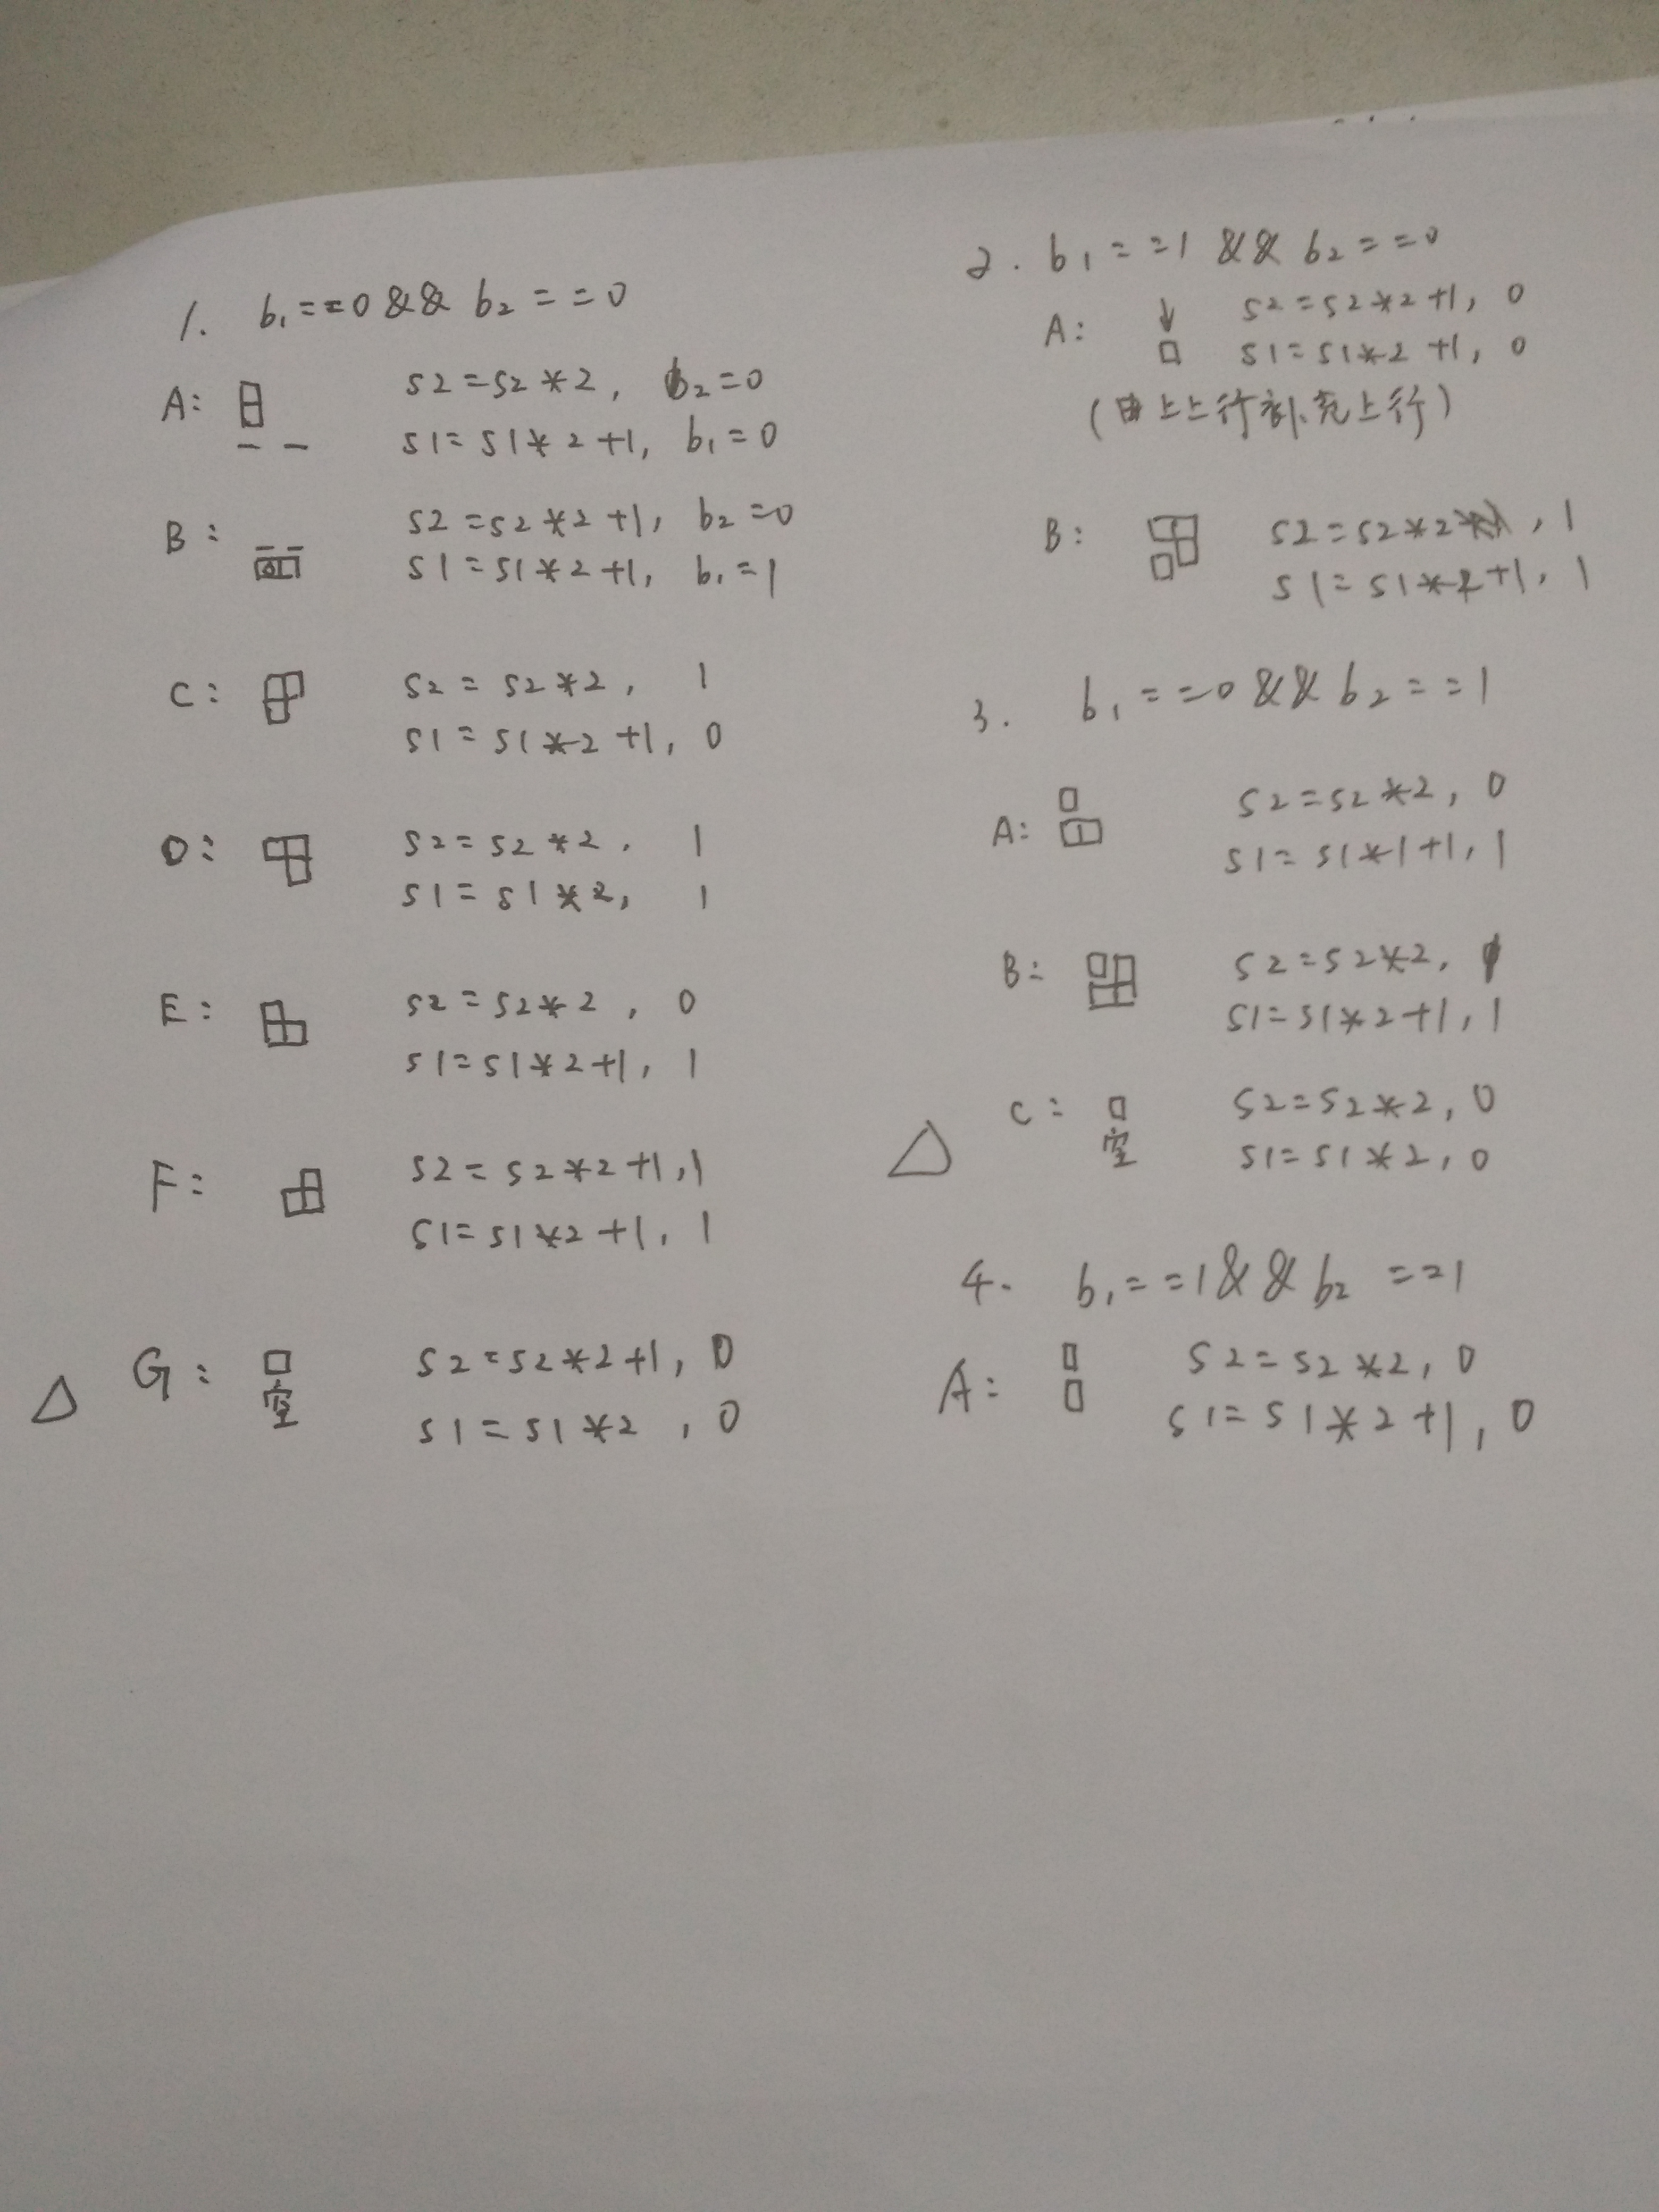
\includegraphics[height = 14cm,width = 17cm]{SCR.jpg}
\begin{lstlisting}
const int MAX_N = 12;

int n, m;
ll ans[MAX_N][MAX_N], dp[MAX_N][1 << MAX_N];

void dfs(int row, int col, int s1, int b1, int s2, int b2)
{
	if (col > m) return;
	if (col == m) {
		if (b1 == 0 && b2 == 0) dp[row][s1] += dp[row - 1][s2];
		return;
	}
	if (b1 == 0 && b2 == 0) {
		dfs(row, col + 1, s1 << 1 | 1, 0, s2 << 1, 0); // 1A
		dfs(row, col + 1, s1 << 1 | 1, 1, s2 << 1 | 1, 0); // 1B
		dfs(row, col + 1, s1 << 1 | 1, 0, s2 << 1, 1); // 1C
		dfs(row, col + 1, s1 << 1 | 1, 1, s2 << 1 | 1, 1); // 1D
		dfs(row, col + 1, s1 << 1 | 1, 1, s2 << 1, 0); // 1E
		dfs(row, col + 1, s1 << 1, 1, s2 << 1, 1); // 1F
		dfs(row, col + 1, s1 << 1, 0, s2 << 1 | 1, 0); // 1G
	} else if (b1 == 1 && b2 == 0) {
		dfs(row, col + 1, s1 << 1 | 1, 0, s2 << 1 | 1, 0); // 2A
		dfs(row, col + 1, s1 << 1 | 1, 1, s2 << 1, 1); // 2B
	} else if (b1 == 0 && b2 == 1) {
		dfs(row, col + 1, s1 << 1 | 1, 1, s2 << 1, 0); // 3A
		dfs(row, col + 1, s1 << 1 | 1, 1, s2 << 1, 1); // 3B
		dfs(row, col + 1, s1 << 1, 0, s2 << 1, 0); // 3C
	} else { // b1 == 1 && b2 == 1
		dfs(row, col + 1, s1 << 1 | 1, 0, s2 << 1, 0); // 4A
	}
}

ll solve()
{
	memset(dp, 0, sizeof (dp));
	dp[0][(1 << m) - 1] = 1;
	for (int i = 1; i <= n + 1; ++i) {
		dfs(i, 0, 0, 0, 0, 0);
	}
	return dp[n][(1 << m) - 1];
}

int main()
{
	memset(ans, -1, sizeof (ans));
	while (~scanf ("%d%d", &n, &m)) {
		if (m > n) swap(n, m);
		if (ans[n][m] != -1) printf("%lld\n", ans[n][m]);
		else {
			ans[n][m] = ans[m][n] = solve();
			printf("%lld\n", ans[n][m]);
		}
	}
	return 0;
}
\end{lstlisting}
\underline {给出$n*m(n,m\leq 10)$的方格棋盘,用$1*r$的长方形骨牌不重叠地覆盖这个棋盘,求覆盖满的方案数。}\\

先考虑$r=3$时的情况。首先,此问题有解当且仅当$m$或$n$能被$3$整除。更一般的结论是:用$1*r$的骨牌覆盖满$m*n$的棋盘,则问题有解当且仅当 $m$或$n$能被$r$整除。当$r=2$时,则对应于例1中$m、n$至少有一个是偶数的条件。 \\
把每一列的状态表示成一个$r$进制数,对于$r=3$,我们用$dp[i][s]$表示把前 $i-2$行覆盖满、第$i-1$和第$i$行覆盖状态为$s$的覆盖方案数。对于第$p$列,$s_p=0$表示$s_{1p}=s_{2p}=0$;$s_{p}=1$表示$s_{1p}=0,s_{2p}=1$;$s_{p} = 2 $表示$s_{1p}=s_{2p}=1$。这样,我们就只保留了必要的状态,空间和时间上都有了改进。当$r= 4$时,可以类推,用四进制表示三行的状态,$r=5$时用五进制……分别写出$r= 2,3,4,5$ 的程序,进行归纳,统一DFS的形式,可以把$DFS(p,s1,s2)$分为两部分:
\begin{lstlisting}
1. for i = 0 to r -1 do
    DFS(p + 1, s1 * r + i, s2 * r + (i + 1) mod r) ;
2. DFS(p + r, s1 * r^r + r^r - 1, s2 * r^r + r^r - 1);
\end{lstlisting}
问题解决。但DFS的这种分部方法是我们归纳猜想得到的,并没有什么道理,其正确性无法保证,我们能否通过某种途径证明它的正确性呢?仍以$r=3$为例。根据上面的讨论,$s_p$取值0到2,表示两行第$p$位的状态,但$s_p$并没有明确的定义。我们**定义$s_p$为这两行的第$p$位从上面一行开始向下连续的1的个数**,这样的定义可以很容易地递推,递推式同上两例没有任何改变,却使得上述DFS方法变得很自然。
\begin{lstlisting}
const int MAX_N = 11;
const int MAX_R = 11;
const int LIMIT = 9800000;

int n, m, r;
ll dp[MAX_N][LIMIT], ans[MAX_N][MAX_N][MAX_R], rr, rm;

void dfs(int row, int col, int s1, int s2)
{
	if (col > m) return;
	if (col == m) {
		dp[row][s1] += dp[row - 1][s2];
		return;
	}
	for (int i = 0; i < r; ++i) {
		dfs(row, col + 1, s1 * r + i, s2 * r + (i + 1) % r);
	}
	dfs(row, col + r, s1 * rr + rr - 1, s2 * rr + rr - 1); // 横着放
}

ll solve()
{
	memset(dp, 0, sizeof (dp));
	rm = rr = 1;
	for (int i = 0; i < r; ++i) { rr *= r; }
	for (int i = 0; i < m; ++i) { rm *= r; }
	dp[0][rm - 1] = 1;
	for (int i = 1; i <= n; ++i) {
		dfs(i, 0, 0, 0);
	}
	return dp[n][rm - 1];
}

int main()
{
	memset(ans, -1, sizeof (ans));
	while (~scanf("%d%d%d", &n, &m, &r)) {
		if (m > n) swap(n, m);
		if (ans[n][m][r] != -1) printf("%lld\n", ans[n][m][r]);
		else if (n * m % r || r > n) printf("0\n");
		else {
			ans[n][m][r] = ans[m][n][r] = solve();
			printf("%lld\n", ans[n][m][r]);
		}
	}
	return 0;
}
\end{lstlisting}

\underline {[PKU 1038]}

给出$m(n\leq 150,m\leq 10)$的棋盘,要在上面放置$2*3$的骨牌,有一些方格无法放置,求最多能放置多少个。\\

根据上例的讨论,此题可以使用三进制来表示状态。$s_p$取值0到2,表示两行第$p$位的状态,**定义$s_p$为这两行的第$p$位从上面一行开始向下连续的1的个数**。我们依旧用$s1$表示当前行状态,$s2$表示上一行状态,$p$表示位置,$num$表示从状态$s1$转移到$s2$能增加的骨牌个数。\\
对于当前行第$p$位,如果放置骨牌,则有两种放置方式:
\begin{enumerate}
\item 竖放,$s1$当前位置$p$及后一个位置$p+1$都为2,s2要求$p$和$p+1$列留空2格,即$p,p+1$列都为0,这样能刚好放置一块骨牌且不留空隙。对应的DFS调用方式:$DFS(p + 2, s1 * 9 + 8, s2 * 9, num + 1)$ ;
\item 横放,$s1$的三个位置都要填满,即$p,p+1,p+2$列均为2,$s2$要求$p,p+1,p+2$列均为1,调用$DFS(p + 3, s1 * 27 + 26, s2 * 27 + 13, num + 1)$
\end{enumerate}
如果第$p$位不放置骨牌,我们还要把$s2$的状态转移到$s1$中以备下次继续转
移。形象地说就是虚填一些方块使得下次放置骨牌可以不留空隙(\underline {也就是填满所有的位置,但是num并不会增加})。对于某一位置,我们可以分3种情况 DFS 以达到目的。
\begin{enumerate}
\item $s1$的当前行空闲,上一行放满。这个状态可以由$s2$的放满状态转移得到:$DFS(p + 1,s1 * 3 + 1, s2 * 3 + 2, num)$
\item $s1$的当前行和上一行都空闲。这个状态可以由$s2$的当前行空闲,上一行放满的状态转移得到:$DFS(p + 1, s1 * 3, s2 * 3 + 1, num)$
\item $s1$的当前行放满。可以由$s2$的放满状态转移得到:$DFS(x + 1, s1 * 3 + 2, s2 * 3 + 2, num)$(放置了1*1的虚骨牌在$s1$的当前位置)
\end{enumerate}
剩下的是关于不能放置的点(黑点)的处理技巧。可以开两个数组$vertical[i][j],horizonal[i][j]$来标志$(i,j)$位置是否能放置竖放和横放骨牌。每次读进一个不能放置的点,对于$vertical[][]$,就把以这个位置为右上角的2*3的六个位置标记掉,对于$horizonal[][]$,就把以这个位置为右上角的3*2的六个位置标记掉,然后在DFS的时候,判断一下就好了。
\begin{lstlisting}
const int MAX_N = 155;
const int MAX_M = 15;
const int MAX_S = 60000;

int T, n, m, K, cur;
int vertical[MAX_N][MAX_M], horizontal[MAX_N][MAX_M];
int dp[MAX_S][2], pw3[MAX_M];

void dfs(int row, int col, int s1, int s2, int num)
{
	if (col > m) return;
	if (col == m) {
		dp[s1][cur] = max(dp[s1][cur], dp[s2][cur ^ 1] + num);
		return;
	}
	if (row >= 2 && vertical[row][col] == 0) { // 竖放
		dfs(row, col + 2, s1 * 9 + 8, s2 * 9, num + 1);
	}
	if (row >= 1 && horizontal[row][col] == 0) { // 横放
		dfs(row, col + 3, s1 * 27 + 26, s2 * 27 + 13, num + 1);
	}
	dfs(row, col + 1, s1 * 3, s2 * 3 + 1, num);
	dfs(row, col + 1, s1 * 3 + 1, s2 * 3 + 2, num);
	dfs(row, col + 1, s1 * 3 + 2, s2 * 3 + 2, num);
}

void solve()
{
	memset(dp, 0, sizeof (dp));
	cur = 0;
	for (int i = 1; i < n; ++i) {
		cur ^= 1;
		dfs(i, 0, 0, 0, 0);
	}
	int ret = 0;
	for (int i = 0; i < pw3[m]; ++i) {
		ret = max(ret, max(dp[i][cur], dp[i][cur ^ 1]));
	}
	printf("%d\n", ret);
}

int main()
{
	pw3[0] = 1;
	for (int i = 1; i < 12; ++i) { pw3[i] = 3 * pw3[i - 1]; }
	scanf("%d", &T);
	while (T--) {
		scanf("%d%d%d", &n, &m, &K);
		memset(vertical, 0, sizeof (vertical));
		memset(horizontal, 0, sizeof (horizontal));
		for (int i = 0; i < K; ++i) {
			int x, y;
			scanf("%d%d", &x, &y);
			x--, y--;
			vertical[x][y] = vertical[x + 1][y] = vertical[x + 2][y] = 1;
			if (y > 0) vertical[x][y - 1] = vertical[x + 1][y - 1]
                                        = vertical[x + 2][y - 1] = 1;
			horizontal[x][y] = horizontal[x + 1][y] = 1;
			if (y > 0) horizontal[x][y - 1] = horizontal[x + 1][y - 1] = 1;
			if (y > 1) horizontal[x][y - 2] = horizontal[x + 1][y - 2] = 1;
		}
		solve();
	}
	return 0;
}
\end{lstlisting}

\subsection{图论模型}
\underline {[HDU 4917]}

给一个$n(n\leq 40)$个顶点和$m(m\leq 20)$个已知拓扑关系的图,求这个图合法的拓扑排序的个数。\\

已知的$m$个拓扑关系会将图分成若干个联通块,但是每个联通块的内部顶点数量不会超过20(因为$m\leq 20$)。我们把一个含有$num$个顶点的连通块内部可以形成的合法拓扑排序的方案数记为$SCR(num)$,当前还剩下$left$个顶点没被确定(包括连通块内的$num$个顶点)那么此时可得的方案数是:$SCR(num)*C[left][num]$,这个组合数的含义其实就是把这$num$个顶点按顺序放在$left$个顶点的任意$num$个位置都是可以的,根据乘法原理,每个连通块的答案要相乘,同时$left$要减掉$num$。 \\
那么剩下来两个问题,如何确定每个连通块内部的顶点和求$SCR(num)$?对于第一个问题,我们可以建立一个0/1邻接矩阵:$child[u][v]$,当$child[u][v]=1$时表示$u$有一个儿子$v$(根据读进来的$m$个关系确定),否则$child[u][v]=0$,对于每个连通块内部点我们可以借鉴\underline {最短路中Floyd算法}的思路,$n^3$的复杂度把这个邻接矩阵“补全”,也就是所有点的所有儿子都标记得到。同一连通块可以通过\underline {并查集}判断得到。同时要把所有的同一连通块中的顶点重新编号。 \\
对于第二个问题,我们同样枚举状态$s: 1\rightarrow ((1 << s) -1)$,把$s$二进制表示中的1看成已经排好序的点,只需要枚举最后一个点是谁,但是要满足\underline {这个点的所有父亲都已经排好序了},把$v$的父亲节点信息同样用一个二进制数$pre[v]$保存就好了,只要状态$s\& pre[v]=pre[v]$,那么就说明状态$s$中包含了所有$v$的父亲。这里是\underline {集合的思想}。 \\
时间复杂度是比较高的:$O(n*2^{num}*num)$,时限给了1000ms,下面的代码跑了795ms。

\begin{lstlisting}
const ll mod = (ll)(1e9 + 7);

int n, m;
int child[45][45], vis[45], fa[45], id[45], step[45], pre[45];
ll dp[1 << 21], C[45][45];

void Floyd()
{
	for (int i = 1; i <= n; ++i) {
		for (int j = 1; j <= n; ++j) {
			if (child[i][j] == 0) continue;
			for (int k = 1; k <= n; ++k) {
				if (child[j][k] == 0) continue;
				child[i][k] = 1;
			}
		}
	}
}

int find(int x)
{
	return fa[x] == x ? x : fa[x] = find(fa[x]);
}

int GetConnectedGraph(int st)
{
	int ret = 0, ancestor = find(st);
	memset(pre, 0, sizeof (pre));
	for (int i = st; i <= n; ++i) {
		if (vis[i]) continue;
		int fi = find(i);
		if (fi == ancestor) {
			id[ret] = i;
			step[i] = ret++;
			vis[i] = 1;
		}
	}
	for (int i = 0; i < ret; ++i) {
		int v = id[i];
		for (int u = 1; u <= n; ++u) {
			if (child[u][v]) {
				pre[v] += (1 << step[u]);
			}
		}
	}
	return ret;
}	

ll SCR(int num)
{
	memset(dp, 0, sizeof (dp));
	dp[0] = 1;
	for (int s = 1; s < (1 << num); ++s) {
		for (int i = 0; i < num; ++i) {
			if ((1 << i) > s) break;
			if ((1 << i) & s) {
				int v = id[i], ss = s - (1 << i);
				int tmp = (pre[v] & ss);
				if (tmp == pre[v]) {
					dp[s] += dp[ss];
					if (dp[s] >= mod) dp[s] -= mod;
				}
			}
		}
	}
	return dp[(1 << num) - 1];
}

ll solve()
{
	Floyd();
	memset(vis, 0, sizeof (vis));
	ll ret = 1;
	int left = n;
	for (int i = 1; i <= n; ++i) {
		if (vis[i]) continue;
		int num = GetConnectedGraph(i);
		ll tmp = SCR(num);
		ret = ret * C[left][num] % mod * tmp % mod;
		left -= num;
	}
	return ret;
}

int main()
{
	for (int i = 0; i < 45; ++i) {
		C[i][0] = C[i][i] = 1;
		for (int j = 1; j < i; ++j) {
			C[i][j] = C[i - 1][j] + C[i - 1][j - 1];
			if (C[i][j] >= mod) C[i][j] -= mod;
		}
	}
	while (~scanf ("%d%d", &n, &m)) {
		memset(child, 0, sizeof (child));
		for (int i = 0; i <= n; ++i) { fa[i] = i; }
		for (int i = 0; i < m; ++i) {
			int u, v, fu, fv;
			scanf("%d%d", &u, &v);
			child[u][v] = 1;
			fu = find(u), fv = find(v);
			if (fu != fv) { fa[fv] = fu; }
		}
		printf("%lld\n", solve());
	}
	return 0;
}
\end{lstlisting}
通过一种DFS的方式获得每个连通块内部的点,并打标记,效果比较好,只跑了592ms。 \\
同样是邻接矩阵$link[i][j]$:
\begin{itemize}
\item $link[i][j]=1:i$是$j$的父亲
\item $link[i][j]=-1:j$是$i$的父亲
\item $link[i][j]=0:i$和$j$不存在直接系
\end{itemize}

\begin{lstlisting}
void dfs(int u, int& num)
{
	id[num] = u;
	vis[u] = 1;
	int tmp = num++; // 暂时保存 u 的编号顺序
	for (int i = 1; i <= n; ++i) {
		if (link[u][i] != 0) { // 父亲方向,儿子方向都遍历
			if (!vis[i]) dfs(i, num); // 遍历 i 的所有儿子和父亲
			if (link[u][i] == 1) { // 遍历 u 的所有儿子
				for (int j = 0; j < num; ++j) {
					if (id[j] == i) { // 找到 i
						pre[j] |= (1 << tmp);
						break;
					}
				}
			}
		}
	}
`}
\end{lstlisting}

\underline {[BZOJ 2784]}

求$n(n\leq 10^5)$以内所有数构成的满足下列条件的集合的个数:如果$x$在这个集合内,那么$2x,3x$都不能在这个集合内。例如:$n=4$,符合条件的子集是:$\{1\},\{1,4\},\{2\},\{2,3\},\{3\},\{3,4\},\{4\}$,一共8个。

需(hen)要(nan)想到这样一个数字矩阵: \\ \\
\begin{tabular}{|c|c|c|c|c|}%开始绘制表格
%{|c|c|c|c|c|} 表示会有5列, 每个的方式未居中(c),
%也可以改成靠左(l)和靠右(r) 其中 | 表示绘制列线
\hline %绘制一条水平的线
x  &  3x &  9x  & 27x  & \dots \\
\hline
2x &  6x & 18x  & 54x  & \dots \\
\hline
4x & 12x & 36x  & 108x & \dots \\
\hline
\dots & \dots & \dots & \dots & \dots \\
\hline
\end{tabular}

这样的数字矩阵最多会有:17行11列。对于每行的数字显然不能取左右相邻的,对于相邻行的状态显然不能同一列都取。每种矩阵方案先构造矩阵,然后状压dp+滚动数组递推,对于所有的可能矩阵方案乘法原理连乘即可。 \\
虽然时限给了10s,但是实际上AC只要660MS。

\begin{lstlisting}
int n;
int mat[18][13], vis[MAX_N], col[18];
ll dp[2][1 << 12];

ll wyr(int x)
{
	int row;
	// 构造矩阵
	for (int i = 1; ; ++i) {
		if (i == 1) mat[i][0] = x;
		else mat[i][0] = 2 * mat[i - 1][0];
		if (mat[i][0] > n) {
			row = i - 1;
			break;
		}
		vis[mat[i][0]] = 1;
		for (int j = 1; ; ++j) {
			mat[i][j] = mat[i][j - 1] * 3;
			if (mat[i][j] > n) {
				col[i] = j; // 每一行的列数
				break;
			}
			vis[mat[i][j]] = 1;
		}
	}
	memset(dp, 0, sizeof (dp));
	dp[0][0] = 1, col[0] = 0;
	int cur = 0;
	ll ret = 0;
	for (int i = 1; i <= row; ++i) {
		cur ^= 1;
		memset(dp[cur], 0, sizeof (dp[cur]));
		for (int s = 0; s < (1 << col[i]); ++s) {
			if (s & (s << 1)) continue; // 同一行不能取相邻
			for (int pre = 0; pre < (1 << col[i - 1]); ++pre) {
				if (dp[cur ^ 1][pre] == 0 || (pre & s)) continue;
				// 上一行状态存在并且不能取相邻列
				dp[cur][s] += dp[cur ^ 1][pre];
				if (dp[cur][s] >= mod) dp[cur][s] -= mod;
			}
			if (i == row) {
				ret += dp[cur][s];
				if (ret >= mod) ret -= mod;
			}
		}
	}
	return ret;
}

int main()
{
	scanf("%d", &n);
	ll ans = 1;
	for (int i = 1; i <= n; ++i) {
		if (vis[i] == 0) {
			ans = ans * wyr(i) % mod;
		}
	}
	printf("%lld\n", ans);
	return 0;
}
\end{lstlisting}

\clearpage
\section{dp优化}

\subsection{二进制优化}
\underline{[HDU 1171]} \\

$n\leq 1000$件商品,每件商品的数量和单价为$num[i]\leq 100$和$value[i]$,求将这些商品尽可能分成价值相等的两部分,输出两部分价值$A$和$B$($A\geq B$)。 \\

把每种商品的数量二级制拆分成“另一种”商品。 \\
将一部分$O(\sum (num[i]))$的时间复杂度降为:$O(\sum{\log (num[i])})$
\begin{lstlisting}
const int MAX_N = 1010;

int sum, n, total;
int value[MAX_N], num[MAX_N], good[MAX_N * 15], dp[100010];

int main()
{
	while (~scanf("%d", &n) && n >= 0) {
		sum = total = 0;
		for (int i = 0; i < n; ++i) {
			scanf("%d%d", &value[i], &num[i]);
			sum += value[i] * num[i];
			for (int j = 1; j <= num[i]; j <<= 1) {
				good[total++] = j * value[i];
				num[i] -= j;
			}
			if (num[i]) good[total++] = num[i] * value[i];
		}
		memset(dp, 0, sizeof (dp));
		dp[0] = 1;
		int half = sum / 2;
		for (int i = 0; i < total; ++i) {
			for (int j = half; j >= good[i]; --j) {
				if (dp[j - good[i]]) {
					dp[j] = 1;
				}
			}
		}
		for (int i = half; i >= 0; --i) {
			if (dp[i]) {
				printf("%d %d\n", sum - i, i);
				break;
			}
		}
	}
	return 0;
}
\end{lstlisting}

\subsection{单调队列优化}
\underline{[POJ 3401]} \\

已知$n\leq 2000$天每天买卖一张股票的单价和买卖上限,但是每天只能选择买或者卖或者不交易,而且两次交易日期中间至少要间隔$W$ 天,最多可以持有$Max$张股票。初始时有无限量的钱,求最终最多可以获利多少? \\

用$dp[i][j]$表示在第$i$天拥有$j$张股票时的最多获利。
\begin{itemize}
\item 第$i$天不买不卖:$dp[i][j]=dp[i - 1][j]$
\item 第$i$天买股票:$dp[i][j]=max(dp[r][k]-cost[i]*(j-k))\quad (r\leq i - W - 1,k< j)$
\item 第$i$天卖股票:$dp[i][j]=max(dp[r][k]+value[i]*(k-j))\quad (r\leq i - W - 1,k> j)$
\end{itemize}
考虑实际意义上面式子中的$r$就应该是$i-W-1$。把第二种情况的状态转移改写一下:
$$
dp[i][j]=(dp[i-W-1][k]+buy[i]*k)-buy[i]*j \qquad (k< j)
$$
可以发现前面部分就是求前缀最大,所以可以用单调队列来保存前缀最大。对于卖股票的行为同样处理,但是因为$k>j$,所以要倒着处理。
\begin{lstlisting}
const int MAX_N = 2010;
const int inf = 0x3f3f3f3f;

int T, n, Max, W, head, tail;
int cost[MAX_N], value[MAX_N], buy[MAX_N], sell[MAX_N];
// cost 和 value: 买卖单价, buy 和 sell: 买卖上限
int dp[MAX_N][MAX_N];

struct Que {
	int num, sum;
	// num: 股票数量 sum: 已经获利量
	Que() {}
	Que(int _num, int _sum): num(_num), sum(_sum) {}
} que[MAX_N];

void wyr()
{
	for (int i = 0; i < n; ++i) memset(dp[i], -0x3f, sizeof (dp[i]));
	// 预处理前 W 天
	for (int j = 0; j <= buy[0]; ++j) { dp[0][j] = -j * cost[0]; }
	for (int i = 1; i <= W; ++i) {
		for (int j = 0; j <= Max; ++j) {
			dp[i][j] = dp[i - 1][j];
			if (j <= buy[i]) dp[i][j] = max(dp[i][j], -j * cost[i]);
		}
	}
	for (int i = W + 1; i < n; ++i) {
		head = tail = 0;
		for (int j = 0; j <= Max; ++j) {
			dp[i][j] = dp[i - 1][j]; // 不买不卖
			
			// 买
			while (head < tail && que[tail - 1].sum <
                                dp[i - W - 1][j] + j * cost[i]) {
				tail--;
			}
			que[tail++] = Que(j, dp[i - W - 1][j] + j * cost[i]);
			// 保证买的数量不超过上限
			while (head < tail && j - que[head].num > buy[i]) head++;
			dp[i][j] = max(dp[i][j], que[head].sum - j * cost[i]);
		}

		head = tail = 0; // 卖
		for (int j = Max; j >= 0; --j) {
			while (head < tail && que[tail - 1].sum <
                            dp[i - W - 1][j] + j * value[i]) {
				tail--;
			}
			que[tail++] = Que(j, dp[i - W - 1][j] + j * value[i]);
			while (head < tail && que[head].num - j > sell[i]) head++;
			dp[i][j] = max(dp[i][j], que[head].sum - j * value[i]);
		}
	}
	int ans = 0;
	for (int i = 0; i <= Max; ++i) {
		ans = max(ans, dp[n - 1][i]);
	}
	printf("%d\n", ans);
}

int main()
{
	scanf("%d", &T);
	while (T--) {
		scanf("%d%d%d", &n, &Max, &W);
		for (int i = 0; i < n; ++i) {
			scanf("%d%d%d%d", &cost[i], &value[i], &buy[i], &sell[i]);
		}
		wyr();
	}
	return 0;
}
\end{lstlisting}

\underline {POJ 3245}

一个长度为$n\leq 5*10^4$的序列(每个元素是($a_i,b_i$)这样的数对),连续地分成若干组。每组左右边界是($l_1,r_1$),($l_2,r_2$),$\cdots$,($l_p,r_p$),满足$l_i=r_{i−1}+1,l_i
\leq r_i,l_1=1,r_p=n$。分组必须满足两个条件:前面组的元素的$b$值比后面组元素的所有$a$值大;令$M_i$为第$i$个组内最大的$a$,所有$M_i$的和不超过$limit$。令$S_i$为第$i$个组的元素的$b$的和,最小化$max\{S_i\}$。 \\

只要有数列后面的$a_j$大于等于当前的$b_i$,那么$i$到$j$的所有元素必须在一个块,那么就把他们合并,合并就是$a$取最大值,$b$取和。此时问题就变成了把这些点分成若干组,且各个组的$M_i$之和要满足限制条件,求$max\{S_i\}$最小是多少,$S_i$表示第$i$组中各个点的$b$值之和。二分$max\{S_i\}$的最小值$x$,然后将问题转变成:将这些点分成若干组,且每组的$b$值之和不能超过$x$,求各个组的$M_i$之和也就各个组的$a$的最大值之和最小是多少,并且判断一下是否小于或等于$limit$。 \\
状态转移方程:
$$
dp[i] = max(dp[j] + max(a[j+1], a[j+2], ..., a[i])) \quad sum[i]-sum[j]\leq M
$$
决策点具有单调性:在决策区间内维护一个单调下降的序列,缩小决策点的数目。需要使用multiset。

时间复杂度:$O(n\log n)$
\begin{lstlisting}
const int MAX_N = 50010;
const int inf = 0x3f3f3f3f;

int n, limit, head, tail;
int A[MAX_N], B[MAX_N], newA[MAX_N], newB[MAX_N], flag[MAX_N];
int pre[MAX_N], suf[MAX_N], sum[MAX_N], dp[MAX_N], Q[MAX_N];
multiset<int> mst;

int check(int x)
{
	dp[0] = Q[0] = head = 0, tail = -1;	
	int st = 1;
	mst.clear();
	for (int i = 1; i <= n; ++i) {
		if (newB[i] > x) return 0;
		while (sum[i] - sum[st - 1] > x) st++; // st 是区间左端点,闭区间
		while (head <= tail && newA[i] >= newA[Q[tail]]) { // 维护队列单调递减性
			if (head < tail) mst.erase(dp[Q[tail - 1]] + newA[Q[tail]]); // 剔除值
			--tail;
		}
		Q[++tail] = i;
		if (head < tail) mst.insert(dp[Q[tail - 1]] + newA[i]); // 增加值
		while (Q[head] < st) { // 将队列首元素位置调到区间内
			if (head < tail) mst.erase(dp[Q[head]] + newA[Q[head + 1]]); // 剔除值
			++head;
		}
		dp[i] = dp[st - 1] + newA[Q[head]]; // 获得 dp 值
		if (head < tail && dp[i] > (*mst.begin())) dp[i] = *mst.begin();
		// mst 中所有值都是 dp[i] 的候选项
		if (dp[i] > limit) return 0;
	}
	return 1;
}

void merge()
{
	suf[n + 1] = 0, pre[0] = INT_MAX;
	for (int i = 1; i <= n; ++i) {
		pre[i] = min(pre[i - 1], B[i]);
	}
	for (int i = n; i >= 1; --i) {
		suf[i] = max(suf[i + 1], A[i]);
	}
	memset(newA, 0, sizeof (newA));
	memset(newB, 0, sizeof (newB));
	memset(flag, 0, sizeof (flag));
	for (int i = 1; i <= n; ++i) {
		if (pre[i] > suf[i + 1]) flag[i] = 1;
	}
	int total = 1;
	for (int i = 1; i <= n; ++i) {
		newA[total] = max(newA[total], A[i]);
		newB[total] += B[i];
		if (flag[i]) total++;
	}
	n = total - 1;
	sum[0] = 0;
	for (int i = 1; i <= n; ++i) {
		sum[i] = sum[i - 1] + newB[i];
	}
}

void solve()
{
	merge();
	int low = 1, high = sum[n], mid;
	while (low < high) {
		mid = (low + high) >> 1;
		if (check(mid)) high = mid;
		else low = mid + 1;
	}
	printf("%d\n", high);
}

int main()
{
	while (~scanf("%d%d", &n, &limit)) {
		for (int i = 1; i <= n; ++i) {
			scanf("%d%d", &A[i], &B[i]);
		}
		solve();
	}
	return 0;
}
\end{lstlisting}

\subsection{斜率优化}
\underline {[POJ 1180]} \\

有$n\leq 10^4$件商品需要加工,每件商品有两个属性:$O(i)$和$F(i)$,可以把连续的一些商品看成一组一起加工,每加工一组需要$S$ 的时间起动机器,假设在时刻$t$开始加工从$i\sim j$的商品,那么加工完这些商品的耗时是:$t+S+\sum_{r=i}^{r=j}{O(r)}=t+T$,需要的代价是:$(t+T)*\sum_{r=i}^{r=j}{F(r)}$,并且下一组的开始时刻是$t+T$,初始时刻是0。求加工完这些商品的最小代价? \\

可以发现每加工完一组商品的这部分时间:$T=S+\sum_{r=i}^{r=j}{O(r)}$对于后面的所有商品都是有影响的,可以先把这部分影响计算累加,影响是:
$$T*\sum_{r=i+1}^{n}{F(r)}=T*fsum(j)$$
于是用$dp[i]$表示加工完$i\sim n$商品的最小代价,$tsum[i]$和$fsum[i]$表示分别$O[]$和$F[]$的后缀和。
$$
dp[i]=min(dp[j]+(S+tsum[i]-tsum[j])*fsum[i])\quad (i< j\leq n)
$$
斜率方程:
$$
\frac{dp[x]-dp[y]}{tsum[x]-tsum[y]}\leq fsum[i]
$$

\begin{lstlisting}
ll G(int x, int y)
{
	return dp[x] - dp[y];
}

ll S(int x, int y)
{
	return tsum[x] - tsum[y];
}

void solve()
{
	head = tail = 0;
	Q[0] = n + 1;
	dp[n + 1] = 0;
	for (int i = n; i >= 1; --i) {
		while (head < tail && G(Q[head + 1], Q[head]) <=
				fsum[i] * S(Q[head + 1], Q[head])) ++head;
		dp[i] = dp[Q[head]] + (tsum[i] - tsum[Q[head]] + s) * fsum[i];
		while (head < tail && G(Q[tail], Q[tail - 1]) * S(i, Q[tail]) >
				G(i, Q[tail]) * S(Q[tail], Q[tail - 1])) --tail;
		Q[++tail] = i;
	}
	printf("%lld\n", dp[1]);
}
\end{lstlisting}

\underline {[HDU 3669]} \\

给出$n\leq 5*10^4$个矩形的长和宽,要求把这些矩形最多分成$K$组,每组的代价是所有这组矩形的最大宽乘以最大长。求最小代价和?\\

先把矩形按照优先宽度:从大到小,其次高度:从大到小的顺序排序,其次要注意到一个事实:如果一个矩形的宽和长都比另外一个矩形小,那个这个矩形就是不用考虑的。因此我们根据排序后的矩形筛选出的矩形序列满足这样性质:宽递减并且长递增。 \\
用$dp[i][k]$表示将前$i$个矩形分成$k$组的最小代价:
$$
dp[i][k]=min(dp[j][k-1]+rec[j+1].w*rec[i].h) \quad (j< i)
$$
斜率方程:
$$
\frac{dp[x][p-1]-dp[y][p-1]}{rec[y+1].w-rec[x+1].w}\leq rec[i].h
$$
\begin{lstlisting}
int n, K, head, tail;
int Q[MAX_N];
ll dp[MAX_N][MAX_K];

struct Rec {
	int w, h;
	bool operator < (const Rec& rhs) const {
		if (w != rhs.w) return w > rhs.w;
		else return h > rhs.h;
	}
} read[MAX_N], rec[MAX_N];

ll G(int id, int x, int y)
{
	return dp[x][id] - dp[y][id];
}

ll S(int x, int y)
{
	return rec[y + 1].w - rec[x + 1].w;
}

void wyr()
{
	for (int i = 1; i <= n; ++i) {
		dp[i][1] = 1ll * rec[1].w * rec[i].h;
	}
	for (int k = 2; k <= K; ++k) {
		head = tail = 0;
		Q[++tail] = k - 1;
		for (int i = k; i <= n; ++i) {
			while (head < tail && G(k - 1, Q[head + 1], Q[head])
					<= S(Q[head + 1], Q[head]) * rec[i].h) ++head;
			int t = Q[head];
			dp[i][k] = dp[t][k - 1] + 1ll * rec[t + 1].w * rec[i].h;
			while (head < tail && G(k - 1, Q[tail], Q[tail - 1]) * S(i, Q[tail])
					>= G(k - 1, i, Q[tail]) * S(Q[tail], Q[tail - 1])) --tail;
			Q[++tail] = i;
		}
	}
	ll ans = (ll)(1e18);
	for (int i = 1; i <= K; ++i) {
		ans = min(ans, dp[n][i]);
	}
	printf("%lld\n", ans);
}

int main()
{
	while (~scanf("%d%d", &n, &K)) {
		for (int i = 0; i < n; ++i) {
			scanf("%d%d", &read[i].w, &read[i].h);
		}
		sort(read, read + n);
		int MaxH = 0, total = 0;
		for (int i = 0; i < n; ++i) {
			if (read[i].h > MaxH) {
				rec[++total].w = read[i].w;
				rec[total].h = read[i].h;
				MaxH = read[i].h;
			}
		}
		n = total;
		wyr();
	}
	return 0;
}
\end{lstlisting}

\subsection{四边形不等式优化}
假如对于$i < j$,有:
$$w(i,j)+w(i+1,j+1)\leq w(i+1,j)+w(i,j+1)$$
称函数$w$满足四边形不等式。 \\
将不等式变形得:
$$
w(i+1,j+1)- w(i+1,j)\leq w(i,j+1) - w(i,j)
$$
那么证明函数$w$是否满足四边形不等式,即证明:当$j$固定不变时是否有:$w(i,j+1)-w(i,j)$随$i$非递增。 \\

\begin{itemize}
\item 定理1 \\
如果有状态转移方程:
$$
m(i,j)=\min_{i < k\leq j}\{ m(i,k-1)+m(k,j)+w(i,j)\} \quad (i < j,m(i,i)=0)
$$
那么函数$m$也满足四边形不等式:
$$
m(i,j)+m(i+1,j+1)\leq m(i+1,j)+m(i,j+1),\quad i < j
$$
\item 定理2 \\
定义$s(i,j)$为函数$m(i,j)$对应的决策变量的最大值,即:
$$
s(i,j)=\max_{i < k\leq j}\{m(i,j)=w(i,j)+m(i,k-1)+m(k,j)\}
$$
并且$m(i,j)$满足四边形不等式,那么$s(i,j)$单调,即:
$$
s(i,j)\leq s(i,j+1)\leq s(i+1,j+1)
$$
因此$m(i,j)$的状态转移方程等价于:
$$
m(i,j)=\min_{s(i,j-1) < k \leq s(i+1,j)}\{ m(i,k-1)+m(k,j)+w(i,j)\} \quad (i < j,m(i,i)=0)
$$
这个转移的复杂度是:$O(n^2)$。
\end{itemize}

\underline {环形石子堆合并} \\

[HDU 3506]:给$n\leq 1000$个围成一圈的石子堆,每次可以合并相邻的两个石子堆成一个新的石子堆,合并的代价是两堆石子数量之和,求将$n$堆石子合并成一堆的最小代价? \\

先将$n$堆环形石子展开成一排$2*n$堆石子。用$dp[i][j]$表示合并第$i$堆到第$j$堆石子的最小代价,状态转移方程:
$$
dp[i][j]=min(dp[i][k]+dp[k+1][j])+cost[i][j]\quad (i\leq k\leq j)
$$
利用四边形不等式优化,只需证明:当$j$固定不变时是否有$cost[i][j+1]-cost[i][j]$随$i$单调非递增。
$$
cost[i][j]=\sum_{r=i}^{r=j}data[r] \\
cost[i][j+1]-cost[i][j]=data[j+1]
$$
因为$j$固定不变,所以差值是个恒定值,那么满足随$i$单调非递增(不变)。 \\
时间复杂度:$O(n^2)$
\begin{lstlisting}
const int MAX_N = 1010 * 2;

int n;
int d[MAX_N], sum[MAX_N];
int dp[MAX_N][MAX_N], s[MAX_N][MAX_N];

void solve()
{
	for (int i = 1; i <= 2 * n; ++i) {
		sum[i] = sum[i - 1] + d[i];
	}
	d[2 * n + 1] = d[1];
	for (int i = 1; i < 2 * n; ++i) {
		dp[i][i + 1] = d[i] + d[i + 1];
		s[i][i + 1] = i;
	}
	for (int len = 3; len <= n; ++len) {
		for (int i = 1; i + len - 1 <= 2 * n; ++i) {
			int j = i + len - 1;
			dp[i][j] = INT_MAX;
			int a = s[i][j - 1], b = s[i + 1][j];
			for (int r = a; r <= b; ++r) {
				int tmp = dp[i][r] + dp[r + 1][j] + sum[j] - sum[i - 1];
				if (tmp < dp[i][j]) {
					dp[i][j] = tmp;
					s[i][j] = r;
				}
			}
		}
	}
	int ans = INT_MAX;
	for (int i = 1; i <= n; ++i) {
		ans = min(ans, dp[i][i + n - 1]);
	}
	printf("%d\n", ans);
}

int main()
{
	while (~scanf("%d", &n)) {
		for (int i = 1; i <= n; ++i) {
			scanf("%d", &d[i]);
			d[i + n] = d[i];
			dp[i][i] = 0;
			s[i][i] = i;
		}
		solve();
	}
	return 0;
}
\end{lstlisting}
\underline {[HDU 2829]}

给$n\leq 1000$个正整数,定义下标$i\sim j$的一串连续的没被挡板隔开的数的价值为:$\sum_{p=i}^{p=j}data[p]\sum_{q=p+1}^{q=j}{data[q]}$,只有一个数时价值为0,选择合适的位置放置$K\in [0,n)$个挡板,使得最终的总价值最小,输出最小总价值。 \\

定义:$sum[i]=\sum_{r=1}^{r=i}{data[r]}$,$fsum[i]=\sum_{r=1}^{r=i}data[r]*sum[r]$
$$
\begin{aligned}
cos[i][j]&=\sum_{p=i}^{p=j}data[p]\sum_{q=p+1}^{q=j}{data[q]} \\
&=\sum_{p=i}^{p=j}data[p]*(sum[j]-sum[p]) \\
&=sum[j]*(sum[j]-sum[i-1])-(fsum[j]-fsum[i-1])
\end{aligned}
$$
定义$dp[i][k]$表示在前$i$个数放置$k$个挡板可获得价值,状态转移方程:
$$
dp[i][k]=\min_{0\leq j < i}\{dp[j][k-1]+cost[j+1][i]\}
$$
考虑四边形不等式优化,只需要证明:当$j$固定时,$cost[i][j+1]-cost[i][j]$随$i$单调非增。
$$
\begin{aligned}
cost[i][j+1]-cost[i][j]&=({sum[j+1]}^{2}-fsum[j+1])-({sum[j]}^{2}-fsum[j]) \\
&+(sum[j]-sum[j+1])*sum[i-1]
\end{aligned}
$$
因为$sum[r]$是单调递增的,所以$(sum[j]-sum[j+1])*sum[i]$在$j$固定的条件下随$i$单调递减,满足四边形不等式优化条件。 \\
时间复杂度:$O(n*K)$,常数有点大
\begin{lstlisting}
const int MAX_N = 1010;

int n, m;
int s[MAX_N][MAX_N];
ll data[MAX_N], sum[MAX_N], fsum[MAX_N];
ll cost[MAX_N][MAX_N], dp[MAX_N][MAX_N];

void wyr()
{
	for (int i = 1; i <= n; ++i) {
		for (int j = i; j <= n; ++j) {
			cost[i][j] = cost[j][i] = sum[j] * (sum[j] - sum[i - 1])
                                - (fsum[j] - fsum[i - 1]);
		}
	}
	memset(dp, 0x3f, sizeof (dp));
	memset(dp[0], 0, sizeof (dp[0]));
	for (int i = 1; i <= n; ++i) {
		dp[i][0] = cost[1][i];
		s[i][0] = 0;
	}
	for (int k = 1; k <= m; ++k) {
		for (int i = n; i >= 1; --i) {
			if (k >= i) dp[i][k] = 0, s[i][k] = i;
			else {
				int a, b;
				if (i == n) a = k - 1, b = n - 1;
				else a = s[i][k - 1], b = s[i + 1][k];
				for (int j = a; j <= b; ++j) {
					if (dp[j][k - 1] + cost[j + 1][i] < dp[i][k]) {
						dp[i][k] = dp[j][k - 1] + cost[j + 1][i];
						s[i][k] = j;
					}
				}
			}
		}
	}
	printf("%lld\n", dp[n][m]);
}

int main()
{
	while (~scanf("%d%d", &n, &m) && (n + m)) {
		for (int i = 1; i <= n; ++i) {
			scanf("%lld", &data[i]);
			sum[i] = sum[i - 1] + data[i];
			fsum[i] = fsum[i - 1] + data[i] * sum[i];
		}
		wyr();
	}
	return 0;
}
\end{lstlisting}
考虑斜率优化。令$k>j$,且:
$$
dp[k][p-1]+cost[k+1][i] < dp[j][p-1]+cost[j+1][i]
$$
即:
$$
\begin{aligned}
dp[k][p-1]+sum[k]*(sum[k]-sum[i-1])-(fsum[k]-fsum[i-1])&< \\
dp[j][p-1]+sum[j]*(sum[j]-sum[i-1])-(fsum[j]-fsum[i-1])
\end{aligned}
$$
化简得斜率方程:
$$
\frac{(dp[k][p-1]+fsum[k])-(dp[j]+fsum[j])}{sum[k]-sum[j]}\leq sum[i]
$$
时间复杂度:$O(n*K)$
\begin{lstlisting}
const int MAX_N = 1010;

int n, K, head, tail;
int Q[MAX_N];
ll data[MAX_N], sum[MAX_N], fsum[MAX_N];
ll dp[MAX_N][MAX_N];

ll G(int id, int x, int y)
{
	return dp[x][id] + fsum[x] - (dp[y][id] + fsum[y]);
}

ll S(int x, int y)
{
	return sum[x] - sum[y];
}

void wyr()
{
	for (int i = 1; i <= n; ++i) {
		dp[i][0] = sum[i] * sum[i] - fsum[i];
	}
	dp[0][0] = 0;
	for (int k = 1; k <= K; ++k) {
		head = tail = 0;
		Q[++tail] = k - 1;
		for (int i = k; i <= n; ++i) {
			while (head < tail && G(k - 1, Q[head + 1], Q[head]) <=
						S(Q[head + 1], Q[head]) * sum[i]) ++head;
			int t = Q[head];
			dp[i][k] = dp[t][k - 1] + sum[i] * (sum[i] - sum[t]) - fsum[i] + fsum[t];
			while (head < tail && G(k - 1, i, Q[tail]) * S(Q[tail], Q[tail - 1]) <=
						G(k - 1, Q[tail], Q[tail - 1]) * S(i, Q[tail])) --tail;
			Q[++tail] = i;
		}
	}
	printf("%lld\n", dp[n][K]);
}

int main()
{
	while (~scanf("%d%d", &n, &K) && (n + K)) {
		for (int i = 1; i <= n; ++i) {
			scanf("%lld", &data[i]);
			sum[i] = sum[i - 1] + data[i];
			fsum[i] = fsum[i - 1] + data[i] * sum[i];
		}
		wyr();
	}
	return 0;
}
\end{lstlisting}

\subsection{bitset优化}
使用bitset优化,利用bitset的位移特性和每一位01表示匹配状态。例如对于模式串:$abc$和读入文本:$abcabcabc$。先根据读入文本得到每个字母向量表示(从右往左看第$i$位为1表示读入文本的第$i$位(从左往右看)为该字母):\\
bs[a]:001001001 \\
bs[b]:010010010 \\
bs[c]:100100100 \\
用dp表示匹配状态,初始时:dp=111111111,扫描模式串:$abc$。 \\

对于第一个字母a,(dp << 1) \& bs[a]可得:dp = (111111110 \& 001001001) = 001001001,这表示字母a可以在文本串中的哪些位置作为前缀。 \\

对于第二个字母b,(dp << 1) \& bs[b]可得:dp = (010010010 \& 010010010) = 010010010,这表示ab可以在文本串中的哪些位置作为前缀。如果想要以当前b结尾作为前缀的话,那么必然需要以前一个字母a作为上一个字母的前缀,所以需要先dp左移一位,然后\underline{与上}当前b可以匹配的位置。\\

对于第三个字母c,(dp << 1) \& bs[c]可得:dp = (100100100 \& 100100100) = 100100100。此时状态1的位置就表示可以和模式串匹配的\underline{结尾位置}。 \\

\underline{[HDU 5745]} \\
给一个长度$n\leq 10^5$的文本串和长度为$m\leq 5000$的模式串,对于文本串的每个字母可以选择相邻位置字母交换但是不允许交叉交换。例如abcd可以变换成bacd,abdc,acbd,badc,但是不能变成bcad,bcda等。对于文本串的每个位置判断以它为起始的子串能否变换成模式串。 \\

其实就是限制了每个位置字母的交换位置只能是相邻的两个。用$dp[i][j][]$表示文本串的第$i$个位置和模式串的第$j$个位置的匹配状态。第三维用0,1,2分别表示文本串的第$i$个字母和第$i-1$个字母交换,不动以及和第$i+1$个字母交换三种状态。状态转移:
$$
\begin{aligned}
dp[i][j][0] &= dp[i-1][j-1][2]\  \&\&\ a[i]==b[j-1] \\
dp[i][j][1] &= (dp[i-1][j-1][0]\ |\ dp[i-1][j][1])\ \&\&\ a[i]==b[j] \\
dp[i][j][2] &= (dp[i-1][j-1][0]\ |\ dp[i-1][j-1][1])\ \&\&\  a[i]==b[j+1]
\end{aligned}
$$
先处理出文本串中每个字母出现的位置,相当于状压第一维,然后枚举模式串的每个位置借助bitset左移操作模拟匹配并且滚动数组。 \\
时间复杂度:$O(\frac{n*m}{w}),w$是机器字节数
\begin{lstlisting}
const int MAX_N = 100010;
const int MAX_M = 5010;

int T, n, m;
int ans[MAX_N];
char str1[MAX_N], str2[MAX_M];
bitset<MAX_N> dp[2][3], bs[30];

void init() {
	for (int i = 0; i < 2; ++i) {
		for (int j = 0; j < 3; ++j) {
			dp[i][j].reset();
			dp[i][j][0] = 1;
		}
	}
	for (int i = 0; i < 26; ++i) { bs[i].reset(); }
	for (int i = 1; i <= n; ++i) {
		bs[str1[i] - 'a'][i] = 1;
	}
}

void solve() {
	init();
	int now = 0;
	dp[0][1].set(); // 初始置为1
	for (int i = 1; i <= m; ++i) {
		now ^= 1;
		if (i > 1) dp[now][0] = (dp[now ^ 1][2] << 1) & bs[str2[i - 1] - 'a'];
		dp[now][1] = ((dp[now ^ 1][1] | dp[now ^ 1][0]) << 1) & bs[str2[i] - 'a'];
		if (i <= m - 1)
            dp[now][2] = ((dp[now ^ 1][0] | dp[now ^ 1][1]) << 1) & bs[str2[i + 1] - 'a'];
		dp[now][0][0] = dp[now][1][0] = dp[now][2][0] = 1;
	}
	for (int i = 1; i <= n - m + 1; ++i) {
		if (dp[now][0][i + m - 1] || dp[now][1][i + m - 1]) printf("1");
		else printf("0");
	}
	for (int i = n - m + 2; i <= n; ++i) { // 最后的 m-1 个位置肯定不符
		printf("0");
	}
	printf("\n");
}

int main() {
	scanf("%d", &T);
	while (T--) {
		scanf("%d%d", &n, &m);
		scanf("%s%s", str1 + 1, str2 + 1);
		solve();
	}
	return 0;
}
\end{lstlisting}

\underline{[2016 大连B]} \\
给一个$n\leq 1000$,代表数字长度,以及每位上候选数字集合,再给一个数字字符串$s(|s|\leq 5*10^{6})$,输出$s$中所有匹配的$n$位数字子串。 \\

样例输入: \\
4 (一共四位) \\
3 0 9 7 (第一位有三个候选数字分别为:0 9 7) \\
2 5 7   (第二位有两个候选数字分别为:5 7) \\
2 2 5   (第三位有两个候选数字分别为:2 5) \\
2 4 5   (第四位有两个候选数字分别为:4 5) \\
09755420524 (数字字符串s) \\

样例输出:(所有匹配的四位数字子串) \\
9755 \\
7554 \\
0524\\

把$n$位数字看成模式串,先处理处每个数字可以在模式串中的匹配位置,然后扫描文本串。用$dp[i][j]$表示文本串的第$i$个位置能否和模式串的第$j$个位置匹配(前缀),状态转移:
$$
\begin{aligned}
dp[i][j]=dp[i-1][j-1]\ \&\&\ a[i]\in b[j]
\end{aligned}
$$
时间复杂度:$O(\frac{n*m}{w}),w$是机器字节数
\begin{lstlisting}
const int MAX_M = 5000010;
const int MAX_N = 1010;

int n, len;
char str[MAX_M];
bitset<MAX_N> bs[10], dp[2];

void solve() {
	len = strlen(str + 1);
	dp[0].reset(), dp[1].reset();
	dp[0][0] = 1;
	int now = 0;
	for (int i = 1; i <= len; ++i) {
		now ^= 1;
		dp[now] = (dp[now ^ 1] << 1) & bs[str[i] - '0'];
		dp[now][0] = 1;
		if (dp[now][n]) {
			char ch = str[i + 1];
			str[i + 1] = '\0';
			printf("%s\n", str + (i - n + 1));
			str[i + 1] = ch;
		}
	}
}

int main() {
	while (~scanf("%d", &n)) {
		for (int i = 0; i < 10; ++i) { bs[i].reset(); }
		for (int i = 1; i <= n; ++i) {
			int x, y;
			scanf("%d", &x);
			for (int j = 0; j < x; ++j) {
				scanf("%d", &y);
				bs[y][i] = 1;
			}
		}
		scanf("%s", str + 1);
		solve();
	}
	return 0;
}
\end{lstlisting}

%\end{document}

%\documentclass[UTF8]{book} % 使用book文档类型格式排版
\usepackage{ctex}  %加载包,因为我们在用中文写文档,所以必须加载这个包,否则不支持中文

%加入了一些针对XeTeX的改进并且加入了 \XeTeX 命令来输入漂亮的XeTeX logo
\usepackage{xltxtra}
%启用一些LaTeX中的功能
\usepackage{xunicode}

\usepackage{multicol}  %加载包
\usepackage{amsmath} % 调用公式宏包
\usepackage{amssymb} % 数学符号生成命令
\usepackage{array} % 数组和表格制作
\usepackage{booktabs} % 绘制水平表格线
\usepackage{calc} %四则运算
\usepackage{caption} % 插图和表格标题格式设置
\usepackage{fancyhdr} % 页眉页脚设置
\usepackage{graphicx} % 调用插图宏包
\usepackage{multicol} % 多栏排版
\usepackage{titlesec} % 章节标题格式设置

%%%% 目录样式 %%%%
\usepackage{titletoc}
\titlecontents{chapter}[1pt]{\vspace{.5\baselineskip}\bfseries}
    {{\thecontentslabel}\quad}{}
    {\hspace{.5em}\titlerule*[10pt]{$\cdot$}\contentspage}
\titlecontents{section}[2em]{\vspace{.25\baselineskip}\bfseries}
    {\thecontentslabel\quad}{}
    {\hspace{.5em}\titlerule*[10pt]{$\cdot$}\contentspage}

\usepackage{color}
\usepackage{xcolor} % 颜色处理
%\usepackage{indentfirst} % 自动首行缩进
%\setlength{\parindent}{2.22em} % 设置首行缩进的距离
% 设置超链接颜色
\usepackage[colorlinks=true,linkcolor=black,urlcolor=black,citecolor=black]{hyperref} % 根据章节标题生成PDF书签

%%%% 版面 %%%%
\usepackage[top=0.5in,bottom=0.5in,left=1.25in,right=0.8in]{geometry}
% 设置行距
\linespread{1}
\usepackage{lscape}
\usepackage{listings} %插入代码,代码页需要加入[fragile]
\usepackage{xeCJK}

%\usepackage[slantfont,boldfont]{xeCJK} % 允许斜体和粗体

%%%% fontspec 宏包 %%%%
\usepackage{fontspec}
% 指定字体
%\setmonofont[Mapping={}]{Monaco}	%英文引号之类的正常显示,相当于设置英文字体
%\setsansfont{Monaco} %设置英文字体 Monaco, Consolas,  Fantasque Sans Mono
%\setmainfont{Monaco} %设置英文字体
% \setCJKmainfont{方正兰亭黑简体}  %中文字体设置
% \setCJKsansfont{华康少女字体} %设置中文字体
% \setCJKmonofont{华康少女字体} %设置中文字体

%%%%%%%%%% 图形支持宏包 %%%%%%%%%%
\usepackage{graphicx}                % 嵌入png图像
\usepackage{color,xcolor}            % 支持彩色文本、底色、文本框等
%\usepackage{subfigure}
%\usepackage{epsfig}                 % 支持eps图像
%\usepackage{picinpar}               % 图表和文字混排宏包
%\usepackage[verbose]{wrapfig}       % 图表和文字混排宏包
%\usepackage{eso-pic}                % 向文档的部分页加n副图形, 可实现水印效果
%\usepackage{eepic}                  % 扩展的绘图支持
%\usepackage{curves}                 % 绘制复杂曲线
%\usepackage{texdraw}                % 增强的绘图工具
%\usepackage{treedoc}                % 树形图绘制
%\usepackage{pictex}                 % 可以画任意的图形
%\usepackage{hyperref}

%\setCJKmainfont{Kai}   % 设置缺省中文字体
%\setCJKmonofont{Hei}   % 设置等宽字体
%\setmainfont{Optima}   % 英文衬线字体
%\setmonofont{Monaco}   % 英文等宽字体
%\setsansfont{Trebuchet MS} % 英文无衬线字体

\makeatletter
\providecommand*\input@path{}
\newcommand\addinputpath[1]{
\expandafter\def\expandafter\input@path
\expandafter{\input@path{#1}}}
\addinputpath{body/}
\makeatother

\definecolor{keywordcolor}{rgb}{0.8,0.1,0.5}
\lstset{language=C++, %用于设置语言为C++
    numbers=left, %设置行号位置
    numberstyle=\tiny, %设置行号大小
    keywordstyle=\color{keywordcolor} \bfseries,
    identifierstyle=,
    basicstyle=\ttfamily,
    commentstyle=\color{blue} \textit, %注释颜色
    stringstyle=\ttfamily,
    showstringspaces=false,
    frame=shadowbox, %边框
    %frame = single,
    tabsize=2, %设置tab空格数
    showspaces=false, %不显示空格
    escapeinside=``, %逃逸字符(1左面的键),用于显示中文
    %breaklines, %自动折行
    captionpos=b
}
%\begin{document}

\chapter{数据结构}

\section{哈希}

\underline{HDU 5918} \\

给定元素个数分别为$n\leq 10^{6}$和$m\leq 10^{6}$的数组$A[]$和$B[]$(下标从1开始)和一个常数$p\leq 10^{6}$,求在数组$A[]$中满足$A[q]=B[1],A[q+p]=B[2],A[q+2*p]=B[3]...,A[q+(m-1)*p]=B[m]$的位置$q(1\leq q, q+(m-1)*p \leq n)$的个数。

\begin{lstlisting}
const ll mod1 = 10341289111ll;
const ll mod2 = 10327287111ll;
const ll prime1 = 95734711;
const ll prime2 = 132134911;
const int MAX_N = 1000010;

int T, n, m, p, cases = 0;
int A[MAX_N], B[MAX_N];

struct Hash {
	ll a, b;
} hesh[MAX_N];

void solve()
{
	ll ret1 = 0, ret2 = 0;
	ll pw1 = 1, pw2 = 1;
	for (int i = 1; i <= m; ++i) {
		ret1 = (ret1 * prime1 % mod1 + B[i]) % mod1;
		if (i > 1) pw1 = pw1 * prime1 % mod1;

		ret2 = (ret2 * prime2 % mod2 + B[i]) % mod2;
		if (i > 1) pw2 = pw2 * prime2 % mod2;
	}
	for (int i = 1; 1ll * (m - 1) * p + i <= n; ++i) {
		if (i <= p) {
			hesh[i].a = hesh[i].b = 0;
			for (int j = 0; j < m; ++j) {
				int pos = i + j * p;
				hesh[i].a = (hesh[i].a * prime1 % mod1 + A[pos]) % mod1;
				hesh[i].b = (hesh[i].b * prime2 % mod2 + A[pos]) % mod2;
			}
		} else {
			hesh[i].a = (hesh[i - p].a - (ll)A[i - p] * pw1 % mod1) * prime1 % mod1;
			hesh[i].a = (hesh[i].a + A[i + (m - 1) * p]) % mod1;
			if (hesh[i].a < 0) hesh[i].a += mod1;

			hesh[i].b = (hesh[i - p].b - (ll)A[i - p] * pw2 % mod2) * prime2 % mod2;
			hesh[i].b = (hesh[i].b + A[i + (m - 1) * p]) % mod2;
			if (hesh[i].b < 0) hesh[i].b += mod2;
		}
	}
	int ans = 0;
	for (int i = 1; 1ll * (m - 1) * p + i <= n; ++i) {
		if (hesh[i].a == ret1 && hesh[i].b == ret2) ans++;
	}
	printf("Case #%d: %d\n", ++cases, ans);
}

int main()
{
	scanf("%d", &T);
	while (T--) {
		scanf("%d%d%d", &n, &m, &p);
		for (int i = 1; i <= n; ++i) {
			scanf("%d", &A[i]);
		}
		for (int i = 1; i <= m; ++i) {
			scanf("%d", &B[i]);
		}
		solve();
	}
	return 0;
}
\end{lstlisting}

\clearpage
\section{并查集}

\subsection{加权并查集}
$n$表示$n$个数字,编号$1–n$,然后有$m$个区间$[l,r]$和该区间和$s$,问在这$m$个区间中有多少个区间和是不正确的? 如果不正确就忽略该区间和,否则将该区间和作为已知条件使用。\\

需要一个数组$val$,$val[i]$表示$i$到根节点的距离,然后就是在查找根节点的过程更新路径上结点的$val$,和在$mix$函数里判断该区间和是否有效。l到$r$之间的和为$s$可以理解为$l$到$r$的距离为$s$。
\begin{lstlisting}
const int maxn = 200010;

int val[maxn], pre[maxn];
int n, m, u, v, w;
//val[i]:i 到根节点的距离; pre[i]:i 的父节点

int find(int x)
{
    if (pre[x] == x) return x;
    int tmp = find(pre[x]); // tmp 是 x 的根节点
    val[x] = val[x] + val[pre[x]];
    // 在递归时 x 还未连接到根节点上,只连接到父节点上,
    // 所以这时的 val[x] 实际上是到父节点的距离
    // 而 val[pre[x]] 是父节点到根节点的距离,
    // 所以真正的 val[x]=val[x]+val[pre[x]], 左边的 val[x] 是到根节点距离,右边的是到父节点距离
    // 可以从递归倒数第二层往前想
    return pre[x] = tmp;//路径压缩
}

int mix(int x, int y, int z)
{
    int fx = find(x), fy = find(y);
    if (fx != fy) {
        pre[fx] = fy; // 将 x 的根节点 fx 的父节点设为fy
        val[fx] = val[y] - val[x] + z;
        // x 到 y 的距离是 z , x 到 fx 的距离是 val[x] , y 到 fy 的距离是 val[y]
        // 那么 fx 到 fy 的距离 val[fx]=x 到 fy 的距离 (z+val[y])- x 到 fx 的距离 val[x]
        return 0;
    } else {
        if (abs(val[y] - val[x]) == z) return 0; // 必须是绝对值才行
        // 因为尽管 y>x ,但是到根节点的距离不确定大小(到根结点路径上个点的值大小不确定)
        return 1;
    }
}

int main()
{
   while (~scanf("%d%d", &n, &m)){
   //因为接下来由 u-- 的存在,所以要从0开始
        for (int i = 0; i <= n; i++)
            pre[i] = i;
        memset(val, 0, sizeof(val));
        int ans = 0;
        for (int i = 1; i <= m; i++) {
            scanf("%d%d%d", &u, &v, &w);
            u--; // 这样做符合 val 的含义
            ans += mix(u, v, w);
        }
        printf("%d\n", ans);
    }
    return 0;
}
\end{lstlisting}

\subsection{分层并查集}

有$n$个动物,编号$1–n$,每个动物属于A,B,C三种中的一种,并且A种动物吃B种动物,B种动物吃C种动物,C种动物吃A种动物。 有$K$ 条语句。格式是:$d,x,y$。
\begin{itemize}
\item $d = 1$时表示$x$和$y$是属于同一种类
\item $d = 2$时表示$x$吃$y$
\end{itemize}
这条语句如果满足下列条件之一就是错误的语句:
\begin{itemize}
\item 当前的话与前面的某些真的话冲突,就是假话;
\item 当前的话中$X$或$Y$比$N$大,就是假话;
\item 当前的话表示$X$吃$X$,就是假话。
\end{itemize}
问$K$条语句中一共有多少条语句是错误的? \\

在数组$pre[3*maxn]$中,$1–n$表示种类A,$n+1–2*n$表示种类B,$2*n+1–3*n$表示种类C。 \\
当$d=1$时:先检查$x$和$y$是否属于不同的种类,如果是不同种类,则$ans++$,否则就将$x$,$y$同属于A,B,C依次$mix$; \\
当$d=2$时:先检查$x$和$y$是否属于同一种类和$y$吃$x$的情况,如果是的,则$ans++$,否则就将$x$属于A,$y$属于B;$x$属于B,$y$属于C;$x$属于C,$y$属于A三种情况$mix$
\begin{lstlisting}
const int maxn = 50010;

int n, k, d, x, y;
int pre[3 * maxn];

int find(int x)
{
    return pre[x] == x ? x : pre[x] = find(pre[x]);
}

void mix(int x, int y)
{
    int fx = find(x), fy = find(y);
    if (fx != fy){
        pre[fx] = fy;
    }
}

int main()
{
    scanf("%d%d", &n, &k);
    for (int i = 1; i <= 3 * n; i++)
        pre[i] = i;
    int ans = 0;
    for (int i = 0; i < k; i++){
        scanf("%d%d%d", &d, &x, &y);
        if (x > n || y > n || (d == 2 && x == y)){
            ans++;
            continue;
        }
        if (d == 1){
            if (find(x) == find(y + n) || find(y) == find(x + n)) ans++;
            // 因为当 x 和 y 属于不同种类时无非是 x 吃 y 或者 y 吃 x
            // 而且每种捕食关系的三种种类归属情况同时入队列,
            //所以检查 x 和 y 属于不同种类就是检查 x 和 y+n 与 x+n 和 y 是否属于同一集合
            // (前者是 x 吃 y ,后者是 y 吃 x )
            else {
                mix(x, y); // 同属A
                mix(x + n, y + n); // 同属 B
                mix(x + 2 * n, y + 2 * n); // 同属 C
            }
        }else {
            if (find(x) == find(y) || find(y) == find(x + n)) ans++;
            //前者是检查 x 和 y 是否属于同一种类,后者是检查是否是 y 吃 x
            else{
                mix(x, y + n); //x 属于 A , y 属于 B
                mix(x + n, y + 2 * n); // x 属于 B , y 属于 C
                mix(x + 2 * n, y); // x属于 C , y 属于 A
            }
        }
    }
    printf("%d\n", ans);
    return 0;
}
\end{lstlisting}

有$n$个数字,每个数字非0即1,有$m$条语句,每条语句:$l,r,even/odd$,表示$l$到$r$区间上有奇/偶个1. 问最多前多少条语句是正确的?\\

用$val[i]$表示从$i$到根节点路径上含有1的数量的奇偶性。在寻找根节点的同时更新路径上的$val$。 \\
比较麻烦的是数据范围:$n<=1000000000,m<=5000$. \\
1.可以用map来标记各个读入点的次序,相当于有个代号,在map里没读入的话就添加进map \\
在$find()$和$mix()$函数里相当于是对代号的操作,代号具有唯一性。 \\
由于$m<=5000$,所以最多会读入10000个相异的数,那么对于$pre$数组和$val$数组都是可以接受的了。 \\
2.$hash$思路。同样是代号的想法,把l(或r) mod maxn 值相同的归在一类,用$head$数组的下标记录这类,head的数值表示最后一类的读入位置。和最短路里链式前向星的查找类似。
\begin{lstlisting}
const int maxn=10010;

int pre[maxn],val[maxn],n,m,l,r,w;
char s[10];

int find(int x)
{
    if(pre[x]==x) return x;
    int tmp=find(pre[x]);
    val[x]=(val[x]+val[pre[x]])%2;
    return pre[x]=tmp;
}

int mix(int x,int y,int z)
{ // 语句正确, mix 返回 1 ,否则返回0
    int fx=find(x);
    int fy=find(y);
    if(fx!=fy)
    {
        pre[fx]=fy;
        val[fx]=(val[y]-val[x]+z)%2;
        return 1;
    }
    else
    {
        if(abs(val[x]-val[y])%2==z) return 1;
        return 0;
    }
}

int main()
{
    while(~scanf("%d",&n)&&n){
        for(int i=0;i<maxn;i++){
            pre[i]=i;
            val[i]=0;
        }
        scanf("%d",&m);
        int ok=0;
        int ans=0;
        int index=0;
        map<int,int> mp;
        for(int i=1;i<=m;i++) {
            scanf("%d%d%s",&l,&r,s);
            if(s[0]=='e') w=0;
            else w=1;
            l--; // 这样做就可以合并相邻的区间,例如:读入 l=1,r=2 和 l=3,r=4
            if(mp.find(l)==mp.end()) mp[l]=index++;
            // find() 函数返回一个迭代器指向键值为 key 的元素
            // 如果没找到就返回指向 map 尾部的迭代器
            if(mp.find(r)==mp.end()) mp[r]=index++;
            // 假设前 x 条语句是正确的,第 x+1 条是错的
            // 那么前 x 次读入 ok 都为 0 ,第 x+1 次读入由于 ok=0,mix() 返回0
            // 所以执行 else 语句, ok 变为 1 , ans=i-1=(x+1)-1=x
            // 从 x+2 开始由于 ok=1 ,不会执行 || 后面的判断,恒continue.
            if(ok||mix(mp[l],mp[r],w)) continue;
            else ok=1;
            if(ok) ans=i-1;
        }
        if(ok==0) ans=m; // 所有的语句都是正确的
        printf("%d\n",ans);
    }
    return 0;
}
\end{lstlisting}

平面上有$n$个点,每个点可以在东西南北四个方向上与另外一个点连接,(每个点最多和四个直接连通) 然后有$m$条语句用以表示这$n$个点之间的位置关系:$a,b,d,S$表示$a$点在$b$点南方,距离为$d(N,W,E$分别表示北,西,东) 接着有$k$条语句来查询:$a,b,t$:由$m$条语句中的前$t$条能否得出$a,b$两点间的哈夫曼距离, 如果由$m$条语句中的前$t$条得出$a,b$两点不连通,则结果为-1. \\

先查询按照查询的t由小到大排序,然后将读入数据读入并查集到相应次序,两个点是否连通可通过$find$来判断。 $x[i],y[i]$分别表示点$i$ 到根节点在横向和竖向的距离。 \\
那么如果$uu,vv$两点连通距离就是$abs(x[uu]-x[vv])+abs(y[uu]-y[vv])$; 但是输出需要按照查询的顺序输出,所以可以把查询语句用结构体存储,并且结构体中一个变量用于存储查询顺序,那么计算每条语句的$ans$时,把查询语句结构体数组按照$t$排序,输出时,再把查询语句按照查询顺序排序输出。
\begin{lstlisting}
const int maxn=40010;
const int maxk=10010;

int pre[maxn],x[maxn],y[maxn],n,m,k,a,b,d,tx,ty;
char ss[10];

struct Query{
    int index,u,v,t,ans;
    // ans 是该条查询语句的答案
}query[maxk];

struct Read{
    int u,v,xx,yy;
}read[maxn];

bool cmp1(Query Q1,Query Q2)
{ //按查询语句的 t 排序
    if(Q1.t==Q2.t) return Q1.index<Q2.index;
    return Q1.t<Q2.t;
}

bool cmp2(Query Q1,Query Q2)
{ //按查询语句的查询顺序排序
    return Q1.index<Q2.index;
}

int find(int u)
{
    if(pre[u]==u) return u;
    int tmp=find(pre[u]);
    x[u]=x[u]+x[pre[u]];
    y[u]=y[u]+y[pre[u]];
    return pre[u]=tmp;
}

void mix(int a,int b,int tx,int ty)
{
    int fa=find(a);
    int fb=find(b);
    if(fa!=fb){
        pre[fa]=fb;
        x[fa]=x[b]-x[a]+tx;
        y[fa]=y[b]-y[a]+ty;
    }
}

int main()
{
    while(~scanf("%d%d",&n,&m)&&n){
        for(int i=0;i<=n;i++)
            pre[i]=i;
        memset(x,0,sizeof(x));
        memset(y,0,sizeof(y));
        for(int i=1;i<=m;i++){
            scanf("%d%d%d%s",&a,&b,&d,ss);
            if(ss[0]=='E'){tx=d;ty=0;} // 这里对方向做了统一规定
            else if(ss[0]=='W'){tx=-d;ty=0;}
            else if(ss[0]=='S'){tx=0;ty=d;}
            else if(ss[0]=='N'){tx=0;ty=-d;}
            read[i].u=a;
            read[i].v=b;
            read[i].xx=tx;
            read[i].yy=ty;
        }
        scanf("%d",&k);
        for(int i=1;i<=k;i++){
            scanf("%d%d%d",&query[i].u,&query[i].v,&query[i].t);
            query[i].ans=0;
            query[i].index=i; //查询顺序标记
        }
        sort(query+1,query+k+1,cmp1);
        int now=1;
        for(int i=1;i<=k;i++){
            for(int j=now;j<=query[i].t;j++){
                a=read[j].u;
                b=read[j].v;
                tx=read[j].xx;
                ty=read[j].yy;
                mix(a,b,tx,ty);
            }
            int uu=query[i].u;
            int vv=query[i].v;
            if(find(uu)==find(vv)) // uu 和 vv 连通{
                query[i].ans=abs(x[uu]-x[vv])+abs(y[uu]-y[vv]);
            }
            else query[i].ans=-1;

            now=query[i].t+1;
        }
        sort(query+1,query+1+k,cmp2);
        for(int i=1;i<=k;i++)
            printf("%d\n",query[i].ans);
    }
    return 0;
}
\end{lstlisting}

有$n$个人玩石头剪刀布,有且只有一个裁判。除了裁判每个人的出拳形式都是一样的。
\begin{itemize}
\item $a<b$表示$b$打败$a$
\item $a=b$表示$a$和$b$出拳一样,平手
\item $a>b$表示$a$打败$b$
\end{itemize}
给出$m$个回合的游戏结果,问能否判断出谁是裁判?如果能还要输出是在哪个回合之后判断出谁是裁判。\\

枚举和加权并查集。\\
对于每个人假设其为裁判,然后去掉所有和他有关的匹配,判断是否会出现矛盾。
\begin{itemize}
\item $val[i]=0$:$i$和根节点属于同一集合
\item $val[i]=1$:根节点打败$i$
\item $val[i]=2$:$i$打败根节点
\end{itemize}
在寻找根节点的$find()$函数中,$val$的更新函数是:$val[x]=(val[x]+val[pre[x]])\%3 $ \\
举个例子:找到根节点之前$val[x]=1$,$val[pre[x]]=2$:表示父节点打败$x$,父节点也打败父节点的父节点。(注意此时$val[x]$是$x$ 与父节点的关系)所以按照递归的思路,从递归倒数第二层开始$pre[x]$就表示为根节点了,那么$pre[x]$打败根节点。又因为$pre[x]$ 也打败$x$所以$val[x]=0=(1+2)\%3$; 递归在往上一层时$pre[x]$又表示为根节点了。 \\
再来看看合并操作时的$val$关系。$fa,fb$分别为$aa,bb$的根节点,$ww$是$aa$与$bb$的关系。 \\
当$fa!=fb$时,令$pre[fa]=fb$.假设$val[aa]=1$,即$fa$打败$aa...(1)$,$val[bb]=2$,即$bb$打败$fb...(2)$,$ww=1$,即$bb$打败$aa...(3)$。则由(1)(2)的$aa$和$fb$是同一集合。再由(1)得$fa$打败$fb$。即$val[fa]=2$.也就是$val[fa]=(val[bb]-val[aa]+ww)\%3$,但是由于有可能$val[bb]-val[aa]+ww<0$,所以正确的方程是:$val[fa]=(val[bb]-val[aa]+ww+3)\%3$.当$fa==fb$时,那么就要判断是否出现矛盾,如果出现矛盾那么说明$i$不能作为裁判。判断矛盾是:$(val[aa]-val[bb]+3)\%3$和$ww$是否相等。如果不矛盾,那么就接着读入输入到最后。

还要注意一点就是可能会出现多个裁判,那就是Can not determine。
\begin{lstlisting}
const int maxn = 510;
const int maxm = 2010;

int n,m,aa,bb,ww;
int pre[maxn],val[maxn];
int line,tmpline, ans,cnt,flag;
char s;

struct Read {
    int a, b, w;
}read[maxm];

void init()
{
    for (int i = 0; i <maxn; i++){
        pre[i] = i;
        val[i]=0;
    }
}

int find(int x)
{
    if(pre[x]==x) return x;
    int tmp=find(pre[x]);
    val[x]=(val[x]+val[pre[x]])%3;
    return pre[x]=tmp;
}

int main()
{
    while (~scanf("%d%d", &n, &m)){
        if (m == 0){
            //printf("case 1\n");
            if(n==1)
     printf("Player 0 can be determined to be the judge after 0 lines\n");
            else printf("Can not determine\n");
            continue;
        }
        for (int i = 0; i<m; i++){
            scanf("%d%c%d", &aa, &s, &bb);
            read[i].a=aa;
            read[i].b=bb;
            if (s == '=') read[i].w=0;
            else if(s=='<') read[i].w=1;
            else if(s=='>') read[i].w=2;
        }
        line=-1;
        cnt=0;
        for(int i=0;i<n;i++)//枚举每个人{
            init();
            tmpline=-1;
            flag=0;
            for(int j=0;j<m;j++) {
                aa=read[j].a;
                bb=read[j].b;
                ww=read[j].w;
                if(aa==i||bb==i) continue;
                //去掉i的影响看是否还会出现矛盾
                int fa=find(aa);
                int fb=find(bb);
                if(fa!=fb){
                    pre[fa]=fb;
                    val[fa]=(val[bb]-val[aa]+ww+3)%3;
                } else{
                    if((val[aa]-val[bb]+3)%3!=ww)//出现矛盾{
                        tmpline=j+1;
                        //出现矛盾所在行
                        flag=1;
                        break;
                    }
                }
                if(flag) break;
            }
            if(flag==0)//没出现矛盾{
                ans=i;//i可以是裁判
                cnt++;
                if(cnt>=2) break;//裁判数量 >=2
            }
            else line=max(line,tmpline);//
        }
        if(cnt==0){
            //printf("case 2\n");
            printf("Impossible\n");
        }else if(cnt>=2){
            //printf("case 3\n");
            printf("Can not determine\n");
        }else{
            //printf("case 4\n");
 printf("Player %d can be determined to be the judge after %d lines\n",ans,line);
        }
    }
    return 0;
}
\end{lstlisting}

\clearpage
\section{$RMQ$}

用于解决区间最值问题,需要$O(n\log n)$的预处理。
\begin{lstlisting}
int n;
int data[MAX_N], dp[MAX_N][20];

void RMQ()
{
	memset(dp, 0, sizeof(dp));
	int k = (int)log2(n * 1.0);
	for (int i = 0; i < n; ++i) { dp[i][0] = data[i]; }
	for (int j = 1; j <= k; ++j) { // 注意枚举顺序
		for (int i = 0; i + (1 << j) - 1 < n; ++i) {
		//一定要 -1 ,因为从 i 开始的第 1<<j 个元素下标是 i + (1 << j) - 1
			int k = i + (1 << (j - 1));
			dp[i][j] = max(dp[i][j - 1], dp[k][j - 1]);
		}
	}
}

// 查询区间 [left, right] 的最值
int len = right - left + 1;
int e = (int)log2(len * 1.0);
int k = right - (1 << e);
res = max(dp[left][e], dp[k][e]);
\end{lstlisting}

\clearpage
\section{线段树}

\subsection{矩形并的周长}

\begin{lstlisting}
#define lson(x) (x<<1)
#define rson(x) ((x<<1)|1)
const int maxn = 5050;
// maxn 是最大矩形数

int n, x1, x2, yy1, y2;
int xx[maxn << 2];

struct SegTree{
    int left, right, len, num, flag;
    // len 是有效长度, num 是有几条线段, flag 记录状态
    bool lcover, rcover;
    // 记录区间左右端点是否存在竖边
}segtree[maxn << 4];

struct Line{
    int x1, x2, y, flag;
    bool operator < (const Line a) const{
        return y < a.y;
    }
}line[maxn << 2];

void build(int left, int right, int cur)
{
    segtree[cur].left = left;
    segtree[cur].right = right;
    segtree[cur].len = segtree[cur].num = segtree[cur].flag = 0;
    segtree[cur].lcover = segtree[cur].rcover = false;
    if(left + 1 == right) return ;
    int mid = (left+right) >> 1;
    build(left, mid, lson(cur));
    build(mid, right, rson(cur));
}

void calc_len(int cur)
{
    int left = segtree[cur].left;
    int right = segtree[cur].right;
    if(segtree[cur].flag > 0){
        segtree[cur].len = xx[right] - xx[left];
        segtree[cur].num = 1;
        segtree[cur].lcover = segtree[cur].rcover = true;
    }else if(left + 1 == right){
        segtree[cur].len = segtree[cur].num = 0;
        segtree[cur].lcover = segtree[cur].rcover = false;
    }else{
        segtree[cur].len = segtree[lson(cur)].len + segtree[rson(cur)].len;
        segtree[cur].num = segtree[lson(cur)].num + segtree[rson(cur)].num;
        segtree[cur].lcover = segtree[lson(cur)].lcover;
        segtree[cur].rcover = segtree[rson(cur)].rcover;
        if(segtree[lson(cur)].rcover && segtree[rson(cur)].lcover)
        // 左右儿子的线段可以衔接
            segtree[cur].num--;//合并成一个线段,所以线段数量-1
    }
    return;
}

void update(int a, int b, int flag, int cur)
{
    int left = segtree[cur].left;
    int right = segtree[cur].right;
    if(left==a && right==b){
        segtree[cur].flag += flag;
        calc_len(cur);
        return;
    }
    if(left + 1 == right) return;
    int mid = (left + right) >> 1;
    if(b <= mid) update(a, b, flag, lson(cur));
    else if(a >= mid) update(a, b, flag, rson(cur));
    else{
        update(a, mid, flag, lson(cur));
        update(mid, b, flag, rson(cur));
    }
    calc_len(cur);
}

int main()
{
    while(~scanf("%d", &n)){
        int tot = 0;
        for(int i = 0; i < n; i++){
            scanf("%d%d%d%d", &x1, &yy1, &x2, &y2);
            line[tot].x1 = x1, line[tot].x2 = x2;
            line[tot].y = yy1, line[tot].flag = 1;
            line[tot+1].x1 = x1, line[tot+1].x2 = x2;
            line[tot+1].y = y2, line[tot+1].flag = -1;
            xx[tot] = x1, xx[tot+1] = x2;
            tot += 2;
        }
        sort(xx, xx + tot);
        int m = unique(xx, xx + tot) - xx;
        build(0, m - 1, 1);
        sort(line, line + tot);
        int ans = 0, last = 0, a, b;
        for(int i=0;i<tot-1;i++){
            a=lower_bound(xx,xx+m,line[i].x1)-xx;
            b=lower_bound(xx,xx+m,line[i].x2)-xx;
            update(a,b,line[i].flag,1);
            ans+=(line[i+1].y-line[i].y)*segtree[1].num*2;
            //竖边数量是线段数量的两倍
            ans+=abs(segtree[1].len-last);
            / /因为加上边时 flag 为 -1 ,这时线段树中这条边就不存在了
            // 但是求周长时是应该加上的
            // 而且在上一棵线段树中是有的,所以要用abs
            last=segtree[1].len;
        }
        a=lower_bound(xx,xx+m,line[tot-1].x1)-xx;
        b=lower_bound(xx,xx+m,line[tot-1].x2)-xx;
        update(a,b,line[tot-1].flag,1);
        ans+=abs(segtree[1].len-last);
        printf("%d\n",ans);
    }
    return 0;
}
\end{lstlisting}

\subsection{矩形交的面积}
\begin{lstlisting}
#define lson(x) (x<<1)
#define rson(x) ((x<<1)|1)
using namespace std;

const int maxn=5050;

int T,n;
double x1,x2,yy1,y2,xx[maxn<<2];

struct SegTree{
    int left,right,flag;
    double len1,len2;
    // len1 是覆盖一次的长度, len2 是覆盖不止一次的长度
}segtree[maxn<<4];

struct Line{
    double x1,x2,y;
    int flag;
    bool operator < (const Line a) const{
        return y<a.y;
    }
}line[maxn<<2];

inline void build(int left,int right,int cur)
{
    segtree[cur].left=left;
    segtree[cur].right=right;
    segtree[cur].flag=0;
    segtree[cur].len1=segtree[cur].len2=0;
    if(left+1==right) return ;
    int mid=(left+right)>>1;
    build(left,mid,lson(cur));
    build(mid,right,rson(cur));
}

inline void calc_len(int cur)
{
    int left=segtree[cur].left;
    int right=segtree[cur].right;
    if(segtree[cur].flag>0) segtree[cur].len1=xx[right]-xx[left];
    else if(left+1==right) segtree[cur].len1=0;
    else segtree[cur].len1=segtree[lson(cur)].len1+segtree[rson(cur)].len1;
    // flag>1 说明整个区间有不止一次覆盖, flag=1 说明整个区间是完全覆盖,
    //但是在这个区间下可能有小区间之前已经被完全覆盖了,所以要加上子树中被覆盖一次的的区间长度
    // flag<1 那么就是左右子树覆盖两次长度之和
    if(segtree[cur].flag>1) segtree[cur].len2=xx[right]-xx[left];
    else if(left+1==right) segtree[cur].len2=0;
    // 叶子结点且 flag<=1 ,则覆盖两次的长度只能是0
    else if(segtree[cur].flag==1)
        segtree[cur].len2=segtree[lson(cur)].len1+segtree[rson(cur)].len1;
    else segtree[cur].len2=segtree[lson(cur)].len2+segtree[rson(cur)].len2;

    return;
}

inline void update(int a,int b,int flag,int cur)
{
    int left=segtree[cur].left;
    int right=segtree[cur].right;
    if(left==a&&right==b){
        segtree[cur].flag+=flag;
        calc_len(cur);
        return;
    }
    if(left + 1 == right) return;
    int mid=(left+right)>>1;
    if(b<=mid) update(a,b,flag,lson(cur));
    else if(a>=mid) update(a,b,flag,rson(cur));
    else{
        update(a,mid,flag,lson(cur));
        update(mid,b,flag,rson(cur));
    }
    calc_len(cur);
}

int main()
{
    scanf("%d",&T);
    while(T--){
        scanf("%d",&n);
        int tot=0;
        for(int i=0;i<n;i++){
            scanf("%lf %lf %lf %lf",&x1,&yy1,&x2,&y2);
            line[tot].x1=x1,line[tot].x2=x2;
            line[tot].y=yy1,line[tot].flag=1;
            line[tot+1].x1=x1,line[tot+1].x2=x2;
            line[tot+1].y=y2,line[tot+1].flag=-1;
            xx[tot]=x1,xx[tot+1]=x2;
            tot+=2;
        }
        sort(xx,xx+tot);
        int m=unique(xx,xx+tot)-xx;
        build(0,m-1,1);
        sort(line,line+tot);
        double ans=0;
        int a,b;
        for(int i=0;i<tot-1;i++){
            a=lower_bound(xx,xx+m,line[i].x1)-xx;
            b=lower_bound(xx,xx+m,line[i].x2)-xx;
            update(a,b,line[i].flag,1);
            //printf("i=%d len=%.2f\n",i,segtree[1].len2);
            ans+=segtree[1].len2*(line[i+1].y-line[i].y);
        }
        printf("%.2f\n",ans);
    }
    return 0;
}
\end{lstlisting}

\subsection{矩形并面积}

\begin{lstlisting}
#define lson(x) (x<<1)
#define rson(x) ((x<<1)|1)
using namespace std;

const int maxn=110;

int n,cases=0;
double x1,x2,yy1,y2,xx[maxn<<2];

struct SegTree{
    int left,right,flag;
    // 只有 flag=1 时该区间才会完全是有效长度
    double len;
}segtree[maxn<<4];

struct Line{
    int flag;
    double x1,x2,y;
    bool operator < (const Line a) const{
        return y<a.y;
    }// 将横边按所在 y 值从小到大排序
}line[maxn<<2];

void build(int left,int right,int cur)
{
    segtree[cur].left=left;
    segtree[cur].right=right;
    segtree[cur].flag=0;
    segtree[cur].len=0;// len 是区间所存的有效横边长度
    if(left+1==right) return;
    int mid=(left+right)>>1;
    build(left,mid,lson(cur));
    build(mid,right,rson(cur));
    // 如果是按照 [left,mid],[mid+1,right] 建树
    // 那么会有一段横坐标 [mid,mid+1] 丢失
}

void calc_len(int cur)
{
    int flag=segtree[cur].flag;
    int left=segtree[cur].left;
    int right=segtree[cur].right;
    if(flag) segtree[cur].len=xx[right]-xx[left];
    // 整个区间长度是区间左右端点所代表的横坐标之差
    else if(left+1==right) segtree[cur].len=0; // 叶子结点且 flag<=0
    else segtree[cur].len=segtree[lson(cur)].len+segtree[rson(cur)].len;
}

void update(int a,int b,int flag,int cur)
{
    int left=segtree[cur].left;
    int right=segtree[cur].right;
    if(left==a&&right==b){
        segtree[cur].flag+=flag;
        calc_len(cur);
        return;
    }
    if(left + 1 == right) return;
    int mid=(left+right)>>1;
    if(b<=mid) update(a,b,flag,lson(cur));
    else if(a>=mid){
        update(a,b,flag,rson(cur));
    }else {
        int mid=(left+right)>>1;
        update(a,mid,flag,lson(cur));
        update(mid,b,flag,rson(cur));
    }
    calc_len(cur);
}

int main()
{
    while((~scanf("%d",&n))&&n){
        int tot=0;
        for(int i=0;i<n;i++){
            scanf("%lf %lf %lf %lf",&x1,&yy1,&x2,&y2);
            xx[tot]=x1,xx[tot+1]=x2;
            line[tot].x1=x1,line[tot].x2=x2;
            line[tot].y=yy1,line[tot].flag=1;
            line[tot+1].x1=x1,line[tot+1].x2=x2;
            line[tot+1].y=y2,line[tot+1].flag=-1;
            tot+=2;
        }
        sort(xx,xx+tot);
        int m=unique(xx,xx+tot)-xx; // 将横坐标去重
        build(0,m-1,1);
        double ans=0;
        sort(line,line+tot);
        //for(int i=0;i<tot;i++)
        //  printf("%lf %lf %lf\n",line[i].x1,line[i].x2,line[i].y);
        for(int i=0;i<tot-1;i++){
            int a=lower_bound(xx,xx+m,line[i].x1)-xx;
            int b=lower_bound(xx,xx+m,line[i].x2)-xx;
            update(a,b,line[i].flag,1);
            ans+=segtree[1].len*(line[i+1].y-line[i].y);
        }
        printf("Test case #%d\n",++cases);
        printf("Total explored area: %.2f\n\n",ans);
    }
    return 0;
}
\end{lstlisting}

\clearpage
\section{树状数组}

\begin{lstlisting}
C[i] = a[i - 2^k + 1] + a[i - 2^k] + ... + a[i];
// k 是 i 二进制表示中末尾连续的 0 的个数

int lowbit(int x)
{
    return x & (-x); // 一个负数的二进制表示与其相反数的二进制之和等于2^32
    // return x & (x ^ (x - 1));
    // return x & (~(x - 1));
}
\end{lstlisting}

\subsection{单点更新,区间求和}
更新所有牵动的区间,求和时求所有区间的所有更新,每个区间覆盖若干子区间但是每个子区间的更新都会体现在父区间中。\\

定理:$A[k]$所牵动的序列为:$C[p_1],C[p_2]...$,其中$p_1=k,p_{i+1}=p_{i}+2^{l_i}(i\geq 1,l_i$指$p_{i}$二进制中末尾0的个数)。\\

典型应用:求逆序对数。\\

\subsection{区间更新,单点求值}
比如区间$[L, R]$要加上$value$,此时数组$C[]$存的是$C$所覆盖的区间改变值之和,那么查询所有覆盖$x$的$C$。\\

区间更新和单点查询复杂度:$O(\log n)$。\\
\subsection{一维区间更新和区间求和}
$C$中记录的是区间该变量,$query(x)$是$data[x]$的该变量,设求$[1, R]$区间和,原数据前缀和为$pre[]$,则:
$$
\begin{aligned}
Ans(R)&=pre[R]+\sum_{i=1}^{R}{query(i)} \\
&=pre[R]+\sum_{i=1}^{i=R}{C[i]*(R-i+1)} \\
&=pre[R]+(R+1)*\sum_{i=1}^{i=R}C[i] - \sum_{i=1}^{i=R}{i*C[i]}
\end{aligned}
$$
另开一个数组$B[i]=i*C[i]$,记录并更新即可。

\begin{lstlisting}
// POJ 3468
int n, m;
ll pre[MAX_N], B[MAX_N], C[MAX_N];

struct BIT {
	ll C[MAX_N], B[MAX_N];

	void init() {
		memset(B, 0, sizeof (B));
		memset(C, 0, sizeof (C));
	}
	int lowbit(const int& x) const {
		return x & (-x);
	}
	ll seg_query(const int& x) const {
		ll ret1 = 0, ret2 = 0;
		for (int i = x; i > 0; i -= lowbit(i)) {
			ret1 += C[i], ret2 += B[i];
		}
		return ret1 * (x + 1) - ret2;
	}
	void seg_update(const int& x, const ll& value)  {
		for (int i = x; i <= n; i += lowbit(i)) {
			C[i] += value, B[i] += value * x; // 注意这里更新 value * x
		}
	}
} bit;

int main()
{
	while (~scanf("%d%d", &n, &m)) {
		bit.init();
		for (int i = 1; i <= n; ++i) {
			ll t;
			scanf("%lld", &t);
			if (i == 1) pre[1] = t;
			else pre[i] = pre[i - 1] + t;
		}
		for (int i = 0; i < m; ++i) {
			char s[10];
			int L, R;
			ll t;
			scanf("%s", s);
			if (s[0] == 'Q') {
				scanf("%d%d", &L, &R);
				printf("%lld\n", bit.seg_query(R) -
                        bit.seg_query(L - 1) + pre[R] - pre[L - 1]);
			} else {
				scanf("%d%d%lld", &L, &R, &t);
				bit.seg_update(L, t);
				bit.seg_update(R + 1, -t);
			}
		}
	}
	return 0;
}
\end{lstlisting}

\subsection{二维区间更新和区间求和}
二维的区间更新和单点求值和一维的类似。

$$
\begin{aligned}
\sum_{i=1}^{i=x}\sum_{j=1}^{j=y}{query(i,j)}
&=\sum_{i=1}^{i=x}\sum_{j=1}^{j=y}{C[i][j]*(x-i+1)*(y-j+1)} \\
&=\sum_{i=1}^{i=x}\sum_{j=1}^{j=y}{C[i][j]*(x+1)*(y+1)} -(y+1)*\sum_{i=1}^{i=x}\sum_{j=1}^{j=y}{i*C[i][j]} \\
&-(x+1)*\sum_{i=1}^{i=x}\sum_{j=1}^{j=y}{j * C[i][j]} +\sum_{i=1}^{i=x}\sum_{j=1}^{j=y}{i*j*C[i][j]}
\end{aligned}
$$

\begin{lstlisting}
// 支持区间更新和区间求和操作,测试BZOJ3132
struct BIT_2D { // 如果必要且空间允许注意开long long
	int row, col; // 矩阵大小
	int B[MAX_N][MAX_N], C[MAX_N][MAX_N], D[MAX_N][MAX_N], E[MAX_N][MAX_N];

	void init() {
		memset(B, 0, sizeof (B));
		memset(C, 0, sizeof (C));
		memset(D, 0, sizeof (D));
		memset(E, 0, sizeof (E));
	}
	int lowbit(const int& x) const {
		return x & (-x);
	}
	void seg_update(const int& x, const int& y, const int& value) {
		for (int i = x; i <= row; i += lowbit(i)) {
			for (int j = y; j <= col; j += lowbit(j)) {
				C[i][j] += value;
				B[i][j] += value * x;
				D[i][j] += value * y;
				E[i][j] += value * x * y;
			}
		}
	}
	int seg_query(const int& x, const int& y) const {
		int ret1 = 0, ret2 = 0, ret3 = 0, ret4 = 0;
		for (int i = x; i > 0; i -= lowbit(i)) {
			for (int j = y; j > 0; j -= lowbit(j)) {
				ret1 += C[i][j], ret2 += B[i][j];
				ret3 += D[i][j], ret4 += E[i][j];
			}
		}
		return ret1 * (x + 1) * (y + 1) - ret2 * (y + 1) - ret3 * (x + 1) + ret4;
	}
} bit;

// 矩阵左上角为 (a, b) 右下角为 (c, d) , 矩阵从上到下从左到右递增
// 查询
ans = bit.seg_query(c, d) + bit.seg_query(a - 1, b - 1);
ans -= (bit.seg_query(a - 1, d) + bit.seg_query(c, b - 1));
printf("%d\n", ans);
// 更新
scanf("%d", &value);
bit.seg_update(a, b, value);
bit.seg_update(c + 1, d + 1, value);
bit.seg_update(a, d + 1, -value);
bit.seg_update(c + 1, b, -value);
\end{lstlisting}

\begin{lstlisting}
// CF341D: 子矩阵中每个元素都异或 value 和查询子矩阵所有元素异或和
int n, m;
ll C[4][MAX_N][MAX_N];

inline int lowbit(int x)
{
	return x & (-x);
}

int GetId(int x, int y)
{
	int ret = 0;
	if (x & 1) ret += 1;
	if (y & 1) ret += 2;
	return ret;
}

void update(int x, int y, ll value)
{
	int id = GetId(x, y);
	for (int i = x; i <= n; i += lowbit(i)) {
		for (int j = y; j <= n; j += lowbit(j)) {
			C[id][i][j] ^= value;
		}
	}
}

ll query(int x, int y)
{
	ll ret = 0;
	int id = GetId(x, y);
	for (int i = x; i > 0; i -= lowbit(i)) {
		for (int j = y; j > 0; j -= lowbit(j)) {
			ret ^= C[id][i][j];
		}
	}
	return ret;
}

int main()
{
	scanf("%d%d", &n, &m);
	for (int i = 0; i < m; ++i) {
		int id, a, b, c, d;
		ll value, ans;
		scanf("%d%d%d%d%d", &id, &a, &b, &c, &d);
		if (id == 1) {
			ans = query(c, d);
			ans ^= query(a - 1, d);
			ans ^= query(c, b - 1);
			ans ^= query(a - 1, b - 1);
			printf("%lld\n", ans);
		} else {
			scanf("%lld", &value);
			update(a, b, value);
			update(c + 1, d + 1, value);
			update(a, d + 1, value);
			update(c + 1, b, value);
		}
	}
	return 0;
}
\end{lstlisting}

\clearpage
\section{树上莫队}
[SPOJ COT2]:给一个$n\leq 4*10^4$个结点的树,每个结点有一个值,$m\leq 10^5$次询问,每次询问$u\sim v$路径上不同整数个数。 \\

先用dfs序把树上表示转化为区间表示,然后把区间分块,每块$\sqrt n$大小,对于每个询问$(u,v)$转换成dfs序上的区间$(L,R)$询问。记$p$为两者的LCA,如果$p=u$ 或者$p=v$,那么$L=\min (left[u], left[v]),R=\max (left[u], left[v])$,否则$L=\min (right[u], right[v]), R=\max (left[u], left[v])$,但是这个时候区间中实际上少了$p$。把区间上的询问按照块排序,莫队更新。

时间复杂度:$O(m\sqrt n)$
\begin{lstlisting}
#include <bits/stdc++.h>
using namespace std;
#define pb push_back
#define mp make_pair
typedef long long ll;
const int MAX_N = 40010;
const int MAX_M = 100010;

int n, m;
ll val[MAX_N], store[MAX_N];
int pos[MAX_N * 2], left[MAX_N], right[MAX_N], be[MAX_N * 2], vis[MAX_N];
int fa[MAX_N][20], depth[MAX_N], ans[MAX_M], num[MAX_N];
vector<int> edge[MAX_N];

struct Query {
    int a, b, anc, L, R, id;

    bool operator < (const Query& rhs) const {
        return pos[L] == pos[rhs.L] ? R < rhs.R : pos[L] < pos[rhs.L];
    }
} ques[MAX_M];

void dfs(int u, int p, int& k, int d) {
    left[u] = ++k, depth[u] = d;
    be[k] = u;
    for (int i = 1; i < 20; ++i) fa[u][i] = fa[fa[u][i - 1]][i - 1];
    for (int i = 0; i < edge[u].size(); ++i) {
        int v = edge[u][i];
        if (v == p) continue;
        fa[v][0] = u;
        dfs(v, u, k, d + 1);
    }
    right[u] = ++k;
    be[k] = u;
}

inline int LCA(int u, int v) {
    if (depth[u] > depth[v]) swap(u, v);
    for (int i = 0; i < 20; ++i) {
        if (((depth[v] - depth[u]) >> i) & 1) v = fa[v][i];
    }
    if (u == v) return v;
    for (int i = 19; i >= 0; --i) {
        if (fa[u][i] != fa[v][i]) u = fa[u][i], v = fa[v][i];
    }
    return fa[u][0];
}

inline void update(int x, int& ret) {
    int id = be[x];
    if (vis[id]) {
        num[val[id]]--;
        if (num[val[id]] == 0) ret--;
        vis[id] = 0;
    } else {
        num[val[id]]++;
        if (num[val[id]] == 1) ret++;
        vis[id] = 1;
    }
}

void solve() {
    int K = 0;
    fa[1][0] = 1;
    dfs(1, -1, K, 1);
    int d = (int)sqrt(n + 0.5);
    for (int i = 1; i <= 2 * n; ++i) pos[i] = (i - 1) / d + 1;
    for (int i = 1; i <= m; ++i) {
        int u = ques[i].a, v = ques[i].b, p;
        ques[i].anc = p = LCA(u, v);
        if (p == u || p == v) {
            ques[i].L = min(left[u], left[v]);
            ques[i].R = max(left[u], left[v]);
        } else {
            ques[i].L = min(right[u], right[v]);
            ques[i].R = max(left[u], left[v]);
        }
    }
    sort(ques + 1, ques + 1 + m);
    memset(num, 0, sizeof (num));
    memset(vis, 0, sizeof (vis));

    int ret = 0, L = 1, R = 0;
    for (int i = 1; i <= m; ++i) {
        while (R > ques[i].R) {
            update(R, ret);
            --R;
        }
        while (R < ques[i].R) {
            ++R;
            update(R, ret);
        }

        while (L < ques[i].L) {
            update(L, ret);
            ++L;
        }
        while (L > ques[i].L) {
            --L;
            update(L, ret);
        }

        if (ques[i].a == ques[i].b) ans[ques[i].id] = 1;
        else if (be[L] == ques[i].anc || be[R] == ques[i].anc) ans[ques[i].id] = ret;
        else {
            update(left[ques[i].anc], ret);
            ans[ques[i].id] = ret;
            update(left[ques[i].anc], ret);
        }
    }
    for (int i = 1; i <= m; ++i) printf("%d\n", ans[i]);
}

int main() {
    scanf("%d%d", &n, &m);
    for (int i = 1; i <= n; ++i) {
        scanf("%lld", &val[i]);
        store[i - 1] = val[i];
        edge[i].clear();
    }
    sort(store, store + n);
    int tot = unique(store, store + n) - store;
    for (int i = 1; i <= n; ++i) {
        val[i] = lower_bound(store, store + tot, val[i]) - store + 1;
    }
    for (int i = 1; i < n; ++i) {
        int a, b;
        scanf("%d%d", &a, &b);
        edge[a].pb(b); edge[b].pb(a);
    }
    for (int i = 1; i <= m; ++i) {
        scanf("%d%d", &ques[i].a, &ques[i].b);
        ques[i].id = i;
    }
    solve();
    return 0;
}
\end{lstlisting}

\clearpage
\section{整体二分}

\subsection{[POJ 2104:区间第$k$小]}

\underline{$n\leq 10^{5}$个数和$m\leq 5000$个询问,每次查询区间$[left,right]$第$k_i$小的数是?} \\

首先对于一次询问可以二分答案,然后通过验证比答案大的数有多少个来不断地缩小答案范围直至得到一个准确的答案。而对于多个询问也可以这么做,只不过对每一个询问都需要判定一下,以决定它被划分到哪一个答案的区间里。这个判定过程就是通过比较比二分的$mid$大的数的个数$num$和$k_i$的大小关系。如果比二分的$mid$小的数的个数$num$小于$k_i$,则需要去寻找的答案一定大于$mid$,这时$k'_{i}=k_{i}-num$。如果$num\geq k_i$,那么需要寻找的答案一定$\leq mid$。直到递归结束。\\
时间复杂度:$O((n+m)*\log ^{2} (n+m)*\log (inf))$

\begin{lstlisting}
typedef long long ll;
const int MAX_N = 100010;
const int MAX_M = 5010;
const int inf = (int)(1e9) + 10;

int n, m;
int ans[MAX_M], bit[MAX_N];

struct Query {
	int type, x, y, k, id;
} Q[MAX_N + MAX_M], Q1[MAX_N + MAX_M], Q2[MAX_N + MAX_M];

inline int lowbit(int x) { return x & (-x); }

inline void update(int x, int value) {
	for (int i = x; i <= n; i += lowbit(i)) {
		bit[i] += value;
	}
}

inline int query(int x) {
	int ret = 0;
	for (int i = x; i > 0; i -= lowbit(i)) {
		ret += bit[i];
	}
	return ret;
}

void solve(int qL, int qR, int L, int R) {
	if (qL > qR) return;
	if (L == R) {
		for (int i = qL; i <= qR; ++i) {
			if (Q[i].type == 2) ans[Q[i].id] = L;
		}
		return;
	}
	int mid = (L + R) >> 1;
	int tp1 = 0, tp2 = 0;
	for (int i = qL; i <= qR; ++i) {
		if (Q[i].type == 1) {
			if (Q[i].x <= mid) {
				update(Q[i].id, Q[i].y); // Q[i].y = 1
				Q1[tp1++] = Q[i];
			} else {
				Q2[tp2++] = Q[i];
			}
		} else {
			int small = query(Q[i].y) - query(Q[i].x - 1);
			if (small >= Q[i].k) Q1[tp1++] = Q[i];
			else {
				Q[i].k -= small;
				Q2[tp2++] = Q[i];
			}
		}
	}
	for (int i = 0; i < tp1; ++i) {
		if (Q1[i].type == 1) update(Q1[i].id, -Q1[i].y);
	}
	memcpy(Q + qL, Q1, tp1 * sizeof (Query));
	memcpy(Q + qL + tp1, Q2, tp2 * sizeof (Query));
	solve(qL, qL + tp1 - 1, L, mid);
	solve(qL + tp1, qR, mid + 1, R);
}

int main() {
	while (~scanf("%d%d", &n, &m)) {
		for (int i = 1; i <= n; ++i) {
			scanf("%d", &Q[i].x);
			Q[i].type = 1, Q[i].y = 1;
			Q[i].id = i;
		}
		for (int i = 1; i <= m; ++i) {
			scanf("%d%d%d", &Q[n + i].x, &Q[n + i].y, &Q[n + i].k);
			Q[n + i].type = 2, Q[n + i].id = i;
		}
		solve(1, n + m, -inf, inf);
		for (int i = 1; i <= m; ++i) {
			printf("%d\n", ans[i]);
		}
	}
	return 0;
}
\end{lstlisting}
\subsection{[BZOJ 3110 第$k$大数]}
$n\leq 50000$个位置,$m\leq 50000$个操作。操作有两种:
\begin{itemize}
\item $1\ a\ b\ c$的形式表示在第$a$个位置到第$b$个位置,每个位置加入一个数$c(abs(c)\leq n)$
\item $2\ a\ b\ c$形式,表示询问从第$a$个位置到第$b$个位置,第$c(c\leq Maxlongint)$大的数是多少?(同一位置可能有多个数)
\end{itemize}

整体二分,对左区间操作1中的$c\leq mid$进行区间每个数都加1,统计数字个数。然后对于右区间的每个操作2进行区间查询数字个数。比较划分。

\begin{lstlisting}
typedef long long ll;
const int MAX_N = 50010;

int n, m;
ll B[MAX_N], C[MAX_N];

struct Query {
	int id, type, a, b, ans;
	ll c;
	bool operator < (const Query& rhs) const {
		return id < rhs.id;
	}
} ques[MAX_N], newq1[MAX_N], newq2[MAX_N];

inline int lowbit(int x) { return x & -x; }

ll query(int x) {
	ll ret1 = 0, ret2 = 0;
	for (int i = x; i > 0; i -= lowbit(i)) {
		ret1 += C[i], ret2 += B[i];
	}
	return ret1 * (x + 1) - ret2;
}

void update(int x, int value) {
	for (int i = x; i <= n; i += lowbit(i)) {
		C[i] += value, B[i] += value * x;
	}
}

void solve(int qL, int qR, int left, int right) {
	if (qL > qR) return;
	if (left == right) {
		for (int i = qL; i <= qR; ++i) {
			if (ques[i].type == 2) ques[i].ans = left;
		}
		return;
	}
	int mid = (left + right) >> 1;	
	int tp1 = 0, tp2 = 0;
	for (int i = qL; i <= qR; ++i) {
		int L = ques[i].a, R = ques[i].b;
		if (ques[i].type == 1) {
			if (ques[i].c <= mid) newq1[tp1++] = ques[i];
			else {
				update(L, 1);
				update(R + 1, -1);
				newq2[tp2++] = ques[i];
			}
		} else {
			ll cnt = query(R) - query(L - 1);
			if (cnt < ques[i].c) {
				ques[i].c -= cnt;
				newq1[tp1++] = ques[i];
			} else {
				newq2[tp2++] = ques[i];
			}
		}
	}
	for (int i = 0; i < tp2; ++i) {
		if (newq2[i].type == 1) {
			update(newq2[i].a, -1);
			update(newq2[i].b + 1, 1);
		}
	}
	memcpy(ques + qL, newq1, tp1 * sizeof (Query));
	memcpy(ques + qL + tp1, newq2, tp2 * sizeof (Query));
	solve(qL, qL + tp1 - 1, left, mid);
	solve(qL + tp1, qR, mid + 1, right);
}

int main() {
	scanf("%d%d", &n, &m);
	for (int i = 1; i <= m; ++i) {
		scanf("%d%d%d%lld", &ques[i].type, &ques[i].a, &ques[i].b, &ques[i].c);
		ques[i].id = i;
	}
	solve(1, m, -n, n);
	sort(ques, ques + m + 1);
	for (int i = 1; i <= m; ++i) {
		if (ques[i].type == 2) {
			printf("%d\n", ques[i].ans);
		}
	}
    return 0;
}
\end{lstlisting}

\clearpage
\section{cdq分治(时间分治)}

cdq分治算法的核心在于:去掉时间的限制,将所有查询要求发生的时刻同化,化动态修改为静态查询。对于某些问题来说可以把某一维的限制通过排序看作时间限制然后运用cdq分治。解决三维偏序问题一般要第一维排序,第二维cdq分治,第三位借用数据结构:树状数组,线段树,平衡树等。\\
1.使用CDQ分治的前提
\begin{itemize}
\item 修改操作对询问的贡献独立,修改操作互不影响
\item 允许使用离线算法
\end{itemize}
2.一般步骤
\begin{itemize}
\item 将整个操作序列分为两个长度相等的部分【分】
\item 递归处理前一部分的子问题 【治1】
\item 计算前一部分的子问题中的修改操作对后一部分子问题的影响 【治2】
\item 递归处理后一部分子问题 【治3】
\end{itemize}
3.分治的复杂度($k$是一个和$n$无关的多项式)
\begin{itemize}
\item $T(n)=2T(\frac{n}{2})+O(kn) \rightarrow T(n)=O(kn \log n)$
\item $T(n)=2T(\frac{n}{2})+O(kn\log n)\rightarrow T(n)=O(kn\log^{2} n)$
\item $T(n)=2T(\frac{n}{2})+O(k)\rightarrow T(n)=O(kn)$
\end{itemize}
\subsection{[NEU 1702 三维逆序对]}
定义点$i\leq j$当且仅当$x_{i}\leq x_{j},y_{i}\leq y_{j},z_{i}\leq z_{j}$。给$n\leq 10^5$个点,对每个点求出小于等于它的点的数量。

\begin{lstlisting}
const int MAX_N = 100010;

int T, n, MaxZ;
int bit[MAX_N], same[MAX_N], ans[MAX_N], Z[MAX_N];

struct Point {
	int x, y, z, id;

	bool operator == (const Point& rhs) const {
		return x == rhs.x && y == rhs.y && z == rhs.z;
	}
} P[MAX_N], Q[MAX_N];

bool xyz(Point a, Point b) {
	if (a.x != b.x) return a.x < b.x;
	if (a.y != b.y) return a.y < b.y;
	return a.z < b.z;
}

bool yzx(Point a, Point b) {
	if (a.y != b.y) return a.y < b.y;
	if (a.z != b.z) return a.z < b.z;
	return a.x < b.x;
}

inline int lowbit(int x) { return x & (-x); }

void update(int x, int value) {
	for (int i = x; i <= MaxZ; i += lowbit(i)) {
		bit[i] += value;
	}
}

int query(int x) {
	int ret = 0;
	for (int i = x; i > 0; i -= lowbit(i)) {
		ret += bit[i];
	}
	return ret;
}

void cdq(int left, int right) {
	if (left == right) return;
	int mid = (left + right) >> 1, xmid = P[mid].x;
	cdq(left, mid);
	int total = 0;
	for (int i = left; i <= right; ++i) {
		Q[total++] = P[i];
	}
	sort(Q, Q + total, yzx);
	for (int i = 0; i < total; ++i) {
		if (Q[i].x <= xmid) update(Q[i].z, 1);
		else {
			ans[Q[i].id] += query(Q[i].z);
		}
	}
	for (int i = 0; i < total; ++i) {
		if (Q[i].x <= xmid) update(Q[i].z, -1);
	}
	cdq(mid + 1, right);
}

int main() {
	scanf("%d", &T);
	while (T--) {
		scanf("%d", &n);
		for (int i = 0; i < n; ++i) {
			scanf("%d%d%d", &P[i].x, &P[i].y, &P[i].z);
			P[i].id = i, Z[i] = P[i].z;
		}
		sort(Z, Z + n);
		MaxZ = unique(Z, Z + n) - Z;
		for (int i = 0; i < n; ++i) {
			P[i].z = lower_bound(Z, Z + MaxZ, P[i].z) - Z + 1;
		}
		sort(P, P + n, xyz);
		for (int i = 0, j = 0; i < n; ) {
			while (j < n && P[i] == P[j]) ++j;
			while (i < j) {
				same[P[i].id] = P[j - 1].id;
				++i;
			}
		}
		for (int i = 0; i < n; ++i) {
			P[i].x = i; // 这一步是必须的
		}
		for (int i = 0; i <= MaxZ; ++i) { bit[i] = 0; }
		for (int i = 0; i < n; ++i) { ans[i] = 0; }
		cdq(0, n - 1);
		for (int i = 0; i < n; ++i) {
			printf("%d\n", ans[same[i]]);
		}
	}
	return 0;
}
\end{lstlisting}
\subsection{[UVALive 6776 三维LIS]}
定义两个点$i$和$j$,如果满足$x_i<x_j,y_i<y_j,z_i<z_j$,那么称:$i<j$,给$n\leq 3*10^{5}$个点计算LIS。 \\

先把所有点的$Z$坐标离散化,然后按照$XYZ$的优先级排序,考虑cdq分治。对于区间$[left,right]$内的点再按照$YZX$的优先级排序,记录下$mid+1$的横坐标,需要特殊处理,借用两棵树状数组。

\begin{lstlisting}
const int MAX_N = 300010;

int n, MaxZ;
int bit[2][MAX_N], dp[MAX_N], Z[MAX_N];

struct Point {
	int x, y, z, id;
} P[MAX_N], Q[MAX_N];

bool xyz(Point a, Point b) {
	if (a.x != b.x) return a.x < b.x;
	if (a.y != b.y) return a.y < b.y;
	return a.z < b.z;
}

bool yzx(Point a, Point b) {
	if (a.y != b.y) return a.y < b.y;
	if (a.z != b.z) return a.z > b.z;
	return a.x > b.x;
}

inline int lowbit(int x) { return x & (-x); }

inline void update(int id, int x, int value) {
	for (int i = x; i <= MaxZ; i += lowbit(i)) {
		bit[id][i] = max(bit[id][i], value);
	}
}

inline int query(int id, int x) {
	int ret = 0;
	for (int i = x; i > 0; i -= lowbit(i)) {
		ret = max(ret, bit[id][i]);
	}
	return ret;
}

void Clear(int id, int x) {
	for (int i = x; i <= MaxZ; i += lowbit(i)) {
		bit[id][i] = 0;
	}
}

void cdq(int left, int right) {
	if (left == right) return;
	int mid = (left + right) >> 1, midX = P[mid + 1].x;
	cdq(left, mid);
	int total = 0;
	for (int i = left; i <= right; ++i) {
		Q[total] = P[i];
		Q[total++].id = i; // 重新编号,以便下面的比较插入和查询
	}
	sort(Q, Q + total, yzx);
	for (int i = 0; i < total; ++i) {
		int pos = Q[i].id, tmp;
		if (pos <= mid) {
			update(0, Q[i].z, dp[pos]);
			if (Q[i].x != midX) update(1, Q[i].z, dp[pos]); // 单独建树
		} else {
			if (Q[i].x != midX) tmp = query(0, Q[i].z - 1);
			else tmp = query(1, Q[i].z - 1);
			dp[pos] = max(dp[pos], tmp + 1);
		}
	}
	for (int i = 0; i < total; ++i) {
		int pos = Q[i].id;
		if (pos <= mid) { // 清空树状数组
			Clear(0, Q[i].z);
			if (Q[i].x != midX) Clear(1, Q[i].z);
		}
	}
	cdq(mid + 1, right);
}

int main() {
	scanf("%d", &n);
	for (int i = 0; i < n; ++i) {
		scanf("%d%d%d", &P[i].x, &P[i].y, &P[i].z);
		dp[i] = 1, P[i].id = i;
		Z[i] = P[i].z;
	}
	sort(Z, Z + n);
	MaxZ = unique(Z, Z + n) - Z;
	for (int i = 0; i < n; ++i) {
		P[i].z = lower_bound(Z, Z + MaxZ, P[i].z) - Z + 1;
	}
	sort(P, P + n, xyz);
	for (int i = 0; i <= MaxZ; ++i) { bit[0][i] = bit[1][i] = 0; }
	cdq(0, n - 1);
	int ans = 0;
	for (int i = 0; i < n; ++i) {
		ans = max(ans, dp[i]);
	}
	printf("%d\n", ans);
	return 0;
}
\end{lstlisting}
\subsection{[BZOJ 3295 动态逆序对]}
$n\leq 10^5$个元素依次删除$m\leq 5*10^4 $个元素,每个元素属于$1\sim n$中间的正整数,求删除元素之前序列有多少个逆序对。\\

首先把删除看成逆序插入。定义$x$表示插入时间,$y$表示在数组中的初始位置,$z$表示元素值的大小,每对逆序对即是三维偏序关系。如果最外层按照$y$排序,对于每个区间$[left,right]$都是可以保证$y$单调递增,然后利用$x$和$mid$的大小关系划分区间。此时在区间$[left,mid]$和$[mid+1,right]$内部都是可以保证$y$单调递增并且子区间$[mid+1,right]$的每一个$x$都是比左区间的每一个$x$大的考虑利用左子区间更新右子区间。
\begin{itemize}
\item 左边数值大的造成的逆序对
\end{itemize}
因为此时子区间内部都是$y$单调递增的,所以可以根据枚举的右子区间$i:mid+1\sim right$的$y$大小来确定是否将左子区间的元素的$z$信息插入树状数组,此时完全不用管$x$信息,因为右子区间的每个元素的$x$都比左子区间的每个元素的$x$都大。在查询的时候,可以查比当前$i$的$z$小的个数,然后用插入的$z$的总个数减一下,就得到$z$大的元素个数了。第一阶段处理完了,需要根据插入“清空”树状数组信息。
\begin{itemize}
\item 右边数小造成的逆序对
\end{itemize}
遍历右子区间$i:right\sim mid+1$,将左子区间的$z$也从后往前插入树状数组,这样子可以保证左子区间$y$大的都插进了树状数组,正常查询即可。\\
时间复杂度:$O(n\log n)$
\begin{lstlisting}
const int MAX_N = 100010;

int n, m;
int bit[MAX_N], vis[MAX_N], pos[MAX_N];
ll ans[MAX_N];

struct Node {
	int x, y, z;
} P[MAX_N], Q[MAX_N];

inline int lowbit(int x) { return x & -x; }

void update(int x, int value) {
	for (int i = x; i <= n; i += lowbit(i)) {
		bit[i] += value;
	}
}

int query(int x) {
	int ret = 0;
	for (int i = x; i > 0; i -= lowbit(i)) {
		ret += bit[i];
	}
	return ret;
}

void cdq(int left, int right) {
	if (left >= right) return;
	int mid = (left + right) >> 1;
	int tp1 = left, tp2 = mid + 1;
	for (int i = left; i <= right; ++i) {
		if (P[i].x <= mid) Q[tp1++] = P[i];
		else Q[tp2++] = P[i];
	}
	tp1 = left;
	for (int i = mid + 1; i <= right; ++i) {
		while (tp1 <= mid && Q[tp1].y < Q[i].y) {
			update(Q[tp1].z, 1);
			tp1++;
		}	
		ans[Q[i].x] += (tp1 - left) - query(Q[i].z - 1);
	}
	for (int i = left; i < tp1; ++i) update(Q[i].z, -1);
	
	tp1 = mid;
	for (int i = right; i >= mid + 1; --i) {
		while (tp1 >= left && Q[tp1].y > Q[i].y) {
			update(Q[tp1].z, 1);
			tp1--;
		}
		ans[Q[i].x] += query(Q[i].z - 1);
	}
	for (int i = mid; i > tp1; --i) update(Q[i].z, -1);
	memcpy(P + left, Q + left, (right - left + 1) * sizeof(Node));
	cdq(left, mid);
	cdq(mid + 1, right);
}

int main() {
	scanf("%d%d", &n, &m);
	for (int i = 1; i <= n; ++i) {
		scanf("%d", &P[i].z);
		P[i].x = 0, P[i].y = i, pos[P[i].z] = i;
	}
	int sz = n, t;
	for (int i = 1; i <= m; ++i) {
		scanf("%d", &t);
		vis[t] = 1;
		P[pos[t]].x = sz--;
	}
	for (int i = 1; i <= n; ++i) {
		if (vis[i]) continue;
		P[pos[i]].x = sz--;
	}
	cdq(1, n);
	for (int i = 1; i <= n; ++i) ans[i] += ans[i - 1];
	for (int i = n; i > n - m; --i) {
		printf("%lld\n", ans[i]);
	}
	return 0;
}
\end{lstlisting}
\subsection{[BZOJ 2244 导弹拦截]}
拦截系统的工作方式:虽然它的第一发炮弹能够到达任意的高度、并且能够拦截任意速度的导弹,但是以后每一发炮弹都不能高于前一发的高度,其拦截的导弹的飞行速度也不能大于前一发。给出$n\leq 5*10^4$枚导弹的高度和速度,求每枚导弹被拦截到的概率。\\

实际上就是求每个元素是三维LIS上结点的概率。方案数可能很大,需要用double存。正反搞两次cdq分别求出以第$i$个元素结尾前半部分的LIS和以第$i$个元素起始后半部分的LIS,利用BIT更新最大长度和方案数。
\begin{lstlisting}
const int MAX_N = 50010;

int n, Max, m;
int Y[MAX_N], Z[MAX_N], sta[MAX_N];
double way[MAX_N];

struct Point {
	int x, y, z, id;
	bool operator < (const Point& rhs) const {
		if (y != rhs.y) return y < rhs.y;
		if (z != rhs.z) return z < rhs.z;
		return x < rhs.x;
	}
} P[MAX_N], Q[MAX_N];

struct Ans {
	int dp[2]; // dp[0]: 以 i 结尾前半部分的 LIS
	// dp[1]: 以 i 起始后半部分的 LIS
	double way[2]; // way[]: 分别是方案数
} ans[MAX_N];

struct Bit {
	int len;
	double sum;

	Bit() {}
	Bit(int _len, double _sum): len(_len), sum(_sum) {}
} bit[MAX_N];

inline int lowbit(int x) { return x & -x; }

void update(int x, int len, double sum) {
	for (int i = x; i <= Max; i += lowbit(i)) {
		if (len > bit[i].len) {
			if (bit[i].len == 0) sta[m++] = i;
			bit[i] = Bit(len, sum);
		} else if (len == bit[i].len) bit[i].sum += sum;
	}
}

Bit query(int x) {
	Bit ret = Bit(0, 0);
	for (int i = x; i > 0; i -= lowbit(i)) {
		if (bit[i].len > ret.len) ret = Bit(bit[i].len, bit[i].sum);
		else if (bit[i].len == ret.len) ret.sum += bit[i].sum;
	}
	return ret;
}

void Clear(int x) {
	for (int i = x; i <= Max; i += lowbit(i)) {
		bit[i] = Bit(0, 0);
	}
}

void cdq(int left, int right, int cur) {
	if (left == right) return;
	int mid = (left + right) >> 1;
	int tp1 = left, tp2 = mid + 1;
	for (int i = left; i <= right; ++i) {
		if (P[i].x <= mid) Q[tp1++] = P[i];
		else Q[tp2++] = P[i];
	}
	memcpy(P + left, Q + left, (right - left + 1) * sizeof (Point));
	cdq(left, mid, cur);
	tp1 = left;
	m = 0;
	for (int i = mid + 1; i <= right; ++i) {
		while (tp1 <= mid && Q[tp1].y <= Q[i].y) {
			update(Q[tp1].z, ans[Q[tp1].id].dp[cur], ans[Q[tp1].id].way[cur]);
			tp1++;
		}
		int pos = Q[i].id;
		Bit tmp = query(Q[i].z);
		if (tmp.len + 1 > ans[pos].dp[cur]) {
			ans[pos].dp[cur] = tmp.len + 1;
			ans[pos].way[cur] = tmp.sum;
		} else if (tmp.len + 1 == ans[pos].dp[cur]) {
			ans[pos].way[cur] += tmp.sum;
		}
	}
	for (int i = tp1 - 1; i >= left; --i) {
		Clear(Q[i].z);
	}
	cdq(mid + 1, right, cur);
	
	tp1 = left, tp2 = mid + 1;
	for (int i = left; i <= right; ++i) {
		if (tp1 <= mid && (tp2 > right ||
			P[tp1] < P[tp2])) Q[i] = P[tp1++];
	   	else Q[i] = P[tp2++];	
	}
	memcpy(P + left, Q + left, (right - left + 1) * sizeof (Point));
	
}

void solve() {
	sort(Z, Z + n); sort(Y, Y + n);
	Max = unique(Z, Z + n) - Z;
	int tot = unique(Y, Y + n) - Y;
	for (int i = 1; i <= n; ++i) {
		P[i].y = lower_bound(Y, Y + tot, P[i].y) - Y;
		P[i].z = lower_bound(Z, Z + Max, P[i].z) - Z;
		P[i].y = tot - P[i].y, P[i].z = Max - P[i].z;
	}
	sort(P + 1, P + n + 1); // yzx
	cdq(1, n, 0);
	for (int i = 1; i <= n; ++i) {
		P[i].x = n - P[i].x + 1;
		P[i].y = tot - P[i].y + 1;
		P[i].z = Max - P[i].z + 1;
	}
	sort(P + 1, P + n + 1); // yzx
	cdq(1, n, 1);
	int len = 0;
	double sum = 0;
	for (int i = 1; i <= n; ++i) {
		if (len < ans[i].dp[0]) {
			len = ans[i].dp[0];
			sum = ans[i].way[0];
		} else if (len == ans[i].dp[0]) {
			sum += ans[i].way[0];
		}
	}
	printf("%d\n", len);
	for (int i = 1; i <= n; ++i) {
		if (i > 1) printf(" ");
		int tmp = ans[i].dp[0] + ans[i].dp[1] - 1;
		if (tmp < len) printf("0");
		else printf("%.5lf", ans[i].way[0] * ans[i].way[1] / sum);
	}
	printf("\n");
}

int main() {
	scanf("%d", &n);
	for (int i = 1; i <= n; ++i) {
		scanf("%d%d", &P[i].y, &P[i].z);
		P[i].x = P[i].id = i;
		Y[i - 1] = P[i].y, Z[i - 1] = P[i].z;
		ans[i].dp[0] = ans[i].dp[1] = 1;
		ans[i].way[0] = ans[i].way[1] = 1;
	}
	solve();
	return 0;
}
\end{lstlisting}
\subsection{[BZOJ 1176 Mokia]}
一个$W*W$的棋盘,每个格子内有一个数,初始时全部为0,现在要求维护两种操作:
\begin{itemize}
\item $1\ x\ y\ z$将格子$(x,y)$内的数加上$z$
\item $2\ x_1\ y_1\ x_2\ y_2$询问矩阵$(x_1,y_1,x_2,y_2)$内所有格子的数的和。
\end{itemize}
操作1$\leq 160000$,操作2$\leq 10000$,$1\leq W\leq 2*10^6$。\\

对于询问矩阵$(x_1,y_1,x_2,y_2)$,根据容斥需要添加三个询问$(x_1-1,y_1-1),(x_2,y_1-1),(x_1-1,y_2)$,和每个询问的符号$flag$,属于哪个询问,每次查询时将答案连同符号累加到所属询问里。\\
离散化后,建立三维偏序:$x_0 < x_1,y_0 < y_1,id_0 < id_1$,需要把所有$< id$的值都加进树状数组,第一维按照优先$x$其次$y$排序,第二维根据$id$进行$cdq$分治,第三维按照$y$插入树状数组并统计。
\begin{lstlisting}
const int MAX_N = 200100;

int S, W, n = 0, Max;
int X[MAX_N], Y[MAX_N];
ll bit[MAX_N];

struct Query {
    int x, y, flag, value;
    int id, be;
    ll ans;

    Query() {}
    Query(int _x, int _y, int _flag, int _id, int _be, ll _ans):
        x(_x), y(_y), flag(_flag), id(_id), be(_be), ans(_ans) {}
    bool operator < (const Query& rhs) const {
        if (x != rhs.x) return x < rhs.x;
        if (y != rhs.y) return y < rhs.y;
        return id < rhs.id;
    }
} ques[MAX_N], newq[MAX_N];

inline int lowbit(int x) { return x & -x; }

void update(int x, int value) {
    for (int i = x; i <= Max; i += lowbit(i)) {
        bit[i] += value;
    }
}

ll query(int x) {
    ll ret = 0;
    for (int i = x; i > 0; i -= lowbit(i)) {
        ret += bit[i];
    }
    return ret;
}

void cdq(int left, int right) {
    if (left == right) return;
    int mid = (left + right) >> 1;
    int tp1 = left, tp2 = mid + 1;
    for (int i = left; i <= right; ++i) {
        if (ques[i].id <= mid) newq[tp1++] = ques[i];
        else newq[tp2++] = ques[i];
    }
    memcpy(ques + left, newq + left, (right - left + 1) * sizeof (Query));
    cdq(left, mid);
    tp1 = left;
    for (int i = mid + 1; i <= right; ++i) {
        if (ques[i].flag != 0) { // not change operation
            while (tp1 <= mid && ques[tp1].x <= ques[i].x){
                if (ques[tp1].flag == 0) { // change operation
                    update(ques[tp1].y, ques[tp1].value);
                }
                tp1++;
            }
        }
        ques[i].ans += query(ques[i].y);
    }
    for (int i = tp1 - 1; i >= left; --i) {
        if (ques[i].flag ==0) {
            update(ques[i].y, -ques[i].value);
        }
    }
    cdq(mid + 1, right);
    tp1 = left, tp2 = mid + 1;
    for (int i = left; i <= right; ++i) {
        if (tp1 <= mid && (tp2 > right ||
            ques[tp1] < ques[tp2]))
            newq[i] = ques[tp1++];
        else newq[i] = ques[tp2++];
    }
    memcpy(ques + left, newq + left, (right - left + 1) * sizeof (Query));
}

bool cmp(const Query& a, const Query& b) {
    return a.id < b.id;
}

int main() {
    scanf("%d%d", &S, &W); // S 无关紧要
    int tot1 = 0, tot2 = 0, type;
    while (1) {
        scanf("%d", &type);
        if (type == 3) break;
        ++n;
        if (type == 1) {
            scanf("%d%d%d", &ques[n].x, &ques[n].y, &ques[n].value);
            ques[n].flag = 0, ques[n].id = n;
            X[tot1++] = ques[n].x, Y[tot2++] = ques[n].y;
        } else {
            int x1, y1, x2, y2;
            scanf("%d%d%d%d", &x1, &y1, &x2, &y2);
            ques[n] = Query(x1 - 1, y1 - 1, 1, n, n + 3, 0);
            ques[n + 1] = Query(x2, y1 - 1, -1, n + 1, n + 3, 0);
            ques[n + 2] = Query(x1 - 1, y2, -1, n + 2, n + 3, 0);
            ques[n + 3] = Query(x2, y2, 2, n + 3, n + 3, 0);
            n += 3;
            X[tot1++] = x2, X[tot1++] = x1 - 1;
            Y[tot2++] = y2, Y[tot2++] = y1 - 1;
        }
    }
    sort(X, X + tot1); sort(Y, Y + tot2);
    tot1 = unique(X, X + tot1) - X;
    tot2 = unique(Y, Y + tot2) - Y;
    for (int i = 1; i <= n; ++i) {
        ques[i].x = lower_bound(X, X + tot1, ques[i].x) - X + 1;
        ques[i].y = lower_bound(Y, Y + tot2, ques[i].y) - Y + 1;
    }
    sort(ques + 1, ques + n + 1);
    Max = tot2;
    cdq(1, n);
    sort(ques + 1, ques + n + 1, cmp);
    for (int i = 1; i <= n; ++i) {
        if (ques[i].flag == 0) continue;
        if (ques[i].flag == 2) {
            printf("%lld\n", ques[i].ans);
        } else {
            int be = ques[i].be;
            ques[be].ans += ques[i].ans * ques[i].flag;
        }
    }
    return 0;
}
\end{lstlisting}
\subsection{[BZOJ 1429 货币兑换Cash]}
给出$n\leq 100000$天每天A和B两个股票的单价$a_i$和$b_i$(买入和卖出价格),购买时A和B两个股票的购买比例$rate$,初始时有$S$元,求$n$天后的最大获利量?\\

用$dp[i]$表示第$i$天可以的最大获利量,$x_i,y_i$分别表示用当天的最大获利量可以获得的A和B两个股票的数量。
$$
\begin{aligned}
dp[i]&=x_i*a_i+y_i*b_i \\
\frac{x_i}{y_i}&=rate_i
\end{aligned}
$$
可以解出对应的$x_i$和$y_i$。考虑$dp$状态转移方程:
$$
dp[i]=max(x_j*a_i+y_j*b_i)\quad (j < i)
$$
转化成斜率,$k$决策优于$j$决策,不妨设$x_k < x_j$有:
$$
x_k*a_i+y_k*b_i > x_j*a_i+y_j*b_i\quad (x_k > x_j) \rightarrow
k_i=-\frac{a_i}{b_i} > \frac{y_k-y_j}{x_k-x_j}
$$
因此需要以$x_k$为关键字维护一个凸线,维护一个点集$(x_k,y_k)$,$x_k$是单调递增的,相邻两点的斜率是单调递减的,相当于一个上凸壳。用左半区间已经更新好的$dp$值求出上凸壳点集,然后用右半区的斜率去切左半区的点集更新$dp$值。左半区间只需要点集$(x,y)$,右半区间只需要斜率$k_i=-\frac{a_i}{b_i}$。处理好左半边时需要保证点集按照坐标排好序,处理右半边时需要保证询问按照斜率排好序,相当于用一系列连续变化的直线去切一些连续点组成的凸壳。

\begin{lstlisting}
const int MAX_N = 100100;
const double eps = 1e-9;
const double inf = 1e18;

int n, S;
int sta[MAX_N];
double ans[MAX_N];

struct Query {
	int id;
	double a, b, rate, k;
	double x, y;
	
	// 按照斜率 k 从大到小排序
	bool operator < (const Query& rhs) const {
		return k > rhs.k;
	}
} Q[MAX_N], P[MAX_N];

double slope(int i, int j) {
	if (j == 0) return -inf;
	if (fabs(P[i].x - P[j].x) <= eps) return inf;
	return (P[i].y - P[j].y) / (P[i].x - P[j].x);
}

void cdq(int left, int right) {
	if (left == right) {
		ans[left] = max(ans[left], ans[left - 1]);
		P[left].x = ans[left] * P[left].rate / (P[left].a * P[left].rate + P[left].b);
		P[left].y = P[left].x / P[left].rate;
		return ;
	}
	int mid = (left + right) >> 1;
	int tp1 = left, tp2 = mid + 1;
	// 按照 id 划分区间
	for (int i = left; i <= right; ++i) {
		if (P[i].id <= mid) Q[tp1++] = P[i];
		else Q[tp2++] = P[i];
	}
	memcpy(P + left, Q + left, (right - left + 1) * sizeof (Query));
	int top = 0;
	cdq(left, mid); // 递归处理左区间
	
	// 从左区间获得上凸壳,此时已经保证左区间点集按照坐标排好序
	for (int i = left; i <= mid; ++i) {
		while (top  > 1 && slope(sta[top], sta[top - 1])
                        <= slope(i, sta[top - 1]) + eps) --top;
		sta[++top] = i;
	}
	sta[++top] = 0; // 添加边界
	
	// 用左区间的凸壳更新右区间,右区间保证斜率从大到小排序
	for (int i = mid + 1, st = 1; i <= right; ++i) {
		while (st < top && P[i].k - slope(sta[st], sta[st + 1]) <= eps) ++st;
		int id =  P[i].id;
		ans[id] = max(ans[id], P[sta[st]].x * P[i].a + P[sta[st]].y * P[i].b);
	}
	cdq(mid + 1, right);

	// 把当前区间 [left, right] 点集按坐标排序
	tp1 = left, tp2 = mid + 1;
	for (int i = left; i <= right; ++i) {
		if (tp1 <= mid && (tp2 > right
			|| P[tp1].x < P[tp2].x
			|| (fabs(P[tp1].x - P[tp2].x) <= eps && P[tp1].y < P[tp2].y))) Q[i] = P[tp1++];
		else Q[i] = P[tp2++];
	}
	memcpy(P + left, Q + left, (right - left + 1) * sizeof (Query));
}

int main() {
	scanf("%d%d", &n, &S);
	ans[0] = S;
	for (int i = 1; i <= n; ++i) {
		scanf("%lf%lf%lf", &P[i].a, &P[i].b, &P[i].rate);
		P[i].k = -P[i].a / P[i].b, P[i].id = i;
		ans[i] = 0;
	}
	sort(P + 1, P + n + 1);
	cdq(1, n);
	printf("%.3lf\n", ans[n]);
	return 0;
}
\end{lstlisting}
\subsection{[BZOJ 2961 共点圆]}
有$n\leq 5*10^5$次操作:
\begin{itemize}
\item $0\ x\ y$表示在坐标系中加入一个以$(x, y)$为圆心且过原点的圆
\item $1\ x\ y$表示询问点$(x,y)$是否在所有已加入的圆的内部(含圆周)
\end{itemize}
对于每次询问输出$Yes$或者$No$,输入保证圆心严格在x轴上方(纵坐标为正),且横坐标非零。\\

一个点$(x_0,y_0)$处于圆心$(x,y)$且过原点的圆内部等价于
$$
(x_0-x)^2+(y_0-y)^2\leq x^2+y^2 \\
2x_0x+2y_{0}y\geq x_{0}^2+y_{0}^2
$$
也就是符合条件的圆心必须位于半平面$2x_0x+2y_0y\geq x_{0}^2+y_{0}^2$内部。当$y_{0}>0$时,可得$y\geq -\frac{x_0}{y_0}*x+\frac{x_{0}^2+y_{0}^2}{y_0}$。不妨考虑求出在与半平面垂直的方向上的投影最小的点,如果这个点也在半平面内那么必然所有的点都在半平面内,只有凸包上的点才会是想要求的点。因此当$y_0>0$时,对所有的圆心求一个下凸包,然后对于每个查询点找到在这个下凸包上面斜率最接近$-\frac{x_0}{y_0}$的圆,只要这个圆心满足条件则所有的圆心都满足条件。当$y_0 <  0$时需要维护上凸包。
\begin{lstlisting}
const int MAX_N = 500010;
const double inf = 1e20;
const double eps = 1e-9;

int n;

struct Point {
	int type, id, flag;
	double x, y, k;
	
	void input() {
		scanf("%d%lf%lf", &type, &x, &y);
	}
	bool operator < (const Point& rhs) const {
		return k < rhs.k;
	}
	double dis(const Point& rhs) const {
		return hypot(x - rhs.x, y - rhs.y);
	}
} P[MAX_N], Q[MAX_N], below[MAX_N], above[MAX_N];

inline double slope(Point a, Point b) {
	if (fabs(a.x - b.x) < eps) return inf;
	else return (a.y - b.y) / (a.x - b.x);
}

void cdq(int left, int right) {
	if (left == right) return;
	int mid = (left + right) >> 1;
	int tp1 = left, tp2 = mid + 1;
	for (int i = left; i <= right; ++i) {
		if (P[i].id <= mid) Q[tp1++] = P[i];
		else Q[tp2++] = P[i];
	}
	memcpy(P + left, Q + left, (right - left + 1) * sizeof (Point));
	cdq(left, mid);
	int tot1 = 0, tot2 = 0;
	for (int i = left; i <= mid; ++i) {
		if (P[i].type) continue;
		while (tot1 > 1 && slope(above[tot1], above[tot1 - 1])
                            < slope(P[i], above[tot1])) tot1--;
		above[++tot1] = P[i];
		while (tot2 > 1 && slope(below[tot2], below[tot2 - 1])
                            > slope(P[i], below[tot2])) tot2--;
		below[++tot2] = P[i];
	}
	int st1 = tot1, st2 = 1;
	for (int i = mid + 1; i <= right; ++i) {
		if (!P[i].type) continue;
		if (P[i].y > 0) {
			while (st2 < tot2 && slope(below[st2], below[st2 + 1]) < P[i].k) ++st2;
			if (st2 <= tot2 && below[st2].dis(P[0]) < below[st2].dis(P[i])) P[i].flag = 0;
		} else {
			while (st1 > 1 && slope(above[st1], above[st1 - 1]) < P[i].k) --st1;
			if (st1 >= 1 && above[st1].dis(P[0]) < above[st1].dis(P[i])) P[i].flag = 0;
		}
	}
	cdq(mid + 1, right);
	tp1 = left, tp2 = mid + 1;
	for (int i = left; i <= right; ++i) {
		if (tp1 <= mid && (tp2 > right
			|| P[tp1].x < P[tp2].x
			|| (fabs(P[tp1].x - P[tp2].x) <= eps && P[tp1].y < P[tp2].y)))
			Q[i] = P[tp1++];
		else Q[i] = P[tp2++];
	}
	memcpy(P + left, Q + left, (right - left + 1) * sizeof (Point));
}

bool cmp(Point a, Point b) {
	return a.id < b.id;
}

int main() {
	P[0].x = 0, P[0].y = 0;
	scanf("%d", &n);
	for (int i = 1; i <= n; ++i) {
		P[i].input();
		P[i].k = -P[i].x / P[i].y;
		P[i].id = i, P[i].flag = 1;
	}
	sort(P + 1, P + n + 1);
	cdq(1, n);
	sort(P + 1, P + n + 1, cmp);
	int first = 1; // 特殊处理询问之前没有圆的情况
	for (int i = 1; i <= n; ++i) {
		if (P[i].type) {
			if (P[i].flag && !first) printf("Yes\n");
			else printf("No\n");
		} else if (first) first = 0;
	}
	return 0;
}
\end{lstlisting}

%\end{document}

%\documentclass[UTF8]{book} % 使用book文档类型格式排版
\usepackage{ctex}  %加载包,因为我们在用中文写文档,所以必须加载这个包,否则不支持中文

%加入了一些针对XeTeX的改进并且加入了 \XeTeX 命令来输入漂亮的XeTeX logo
\usepackage{xltxtra}
%启用一些LaTeX中的功能
\usepackage{xunicode}

\usepackage{multicol}  %加载包
\usepackage{amsmath} % 调用公式宏包
\usepackage{amssymb} % 数学符号生成命令
\usepackage{array} % 数组和表格制作
\usepackage{booktabs} % 绘制水平表格线
\usepackage{calc} %四则运算
\usepackage{caption} % 插图和表格标题格式设置
\usepackage{fancyhdr} % 页眉页脚设置
\usepackage{graphicx} % 调用插图宏包
\usepackage{multicol} % 多栏排版
\usepackage{titlesec} % 章节标题格式设置

%%%% 目录样式 %%%%
\usepackage{titletoc}
\titlecontents{chapter}[1pt]{\vspace{.5\baselineskip}\bfseries}
    {{\thecontentslabel}\quad}{}
    {\hspace{.5em}\titlerule*[10pt]{$\cdot$}\contentspage}
\titlecontents{section}[2em]{\vspace{.25\baselineskip}\bfseries}
    {\thecontentslabel\quad}{}
    {\hspace{.5em}\titlerule*[10pt]{$\cdot$}\contentspage}

\usepackage{color}
\usepackage{xcolor} % 颜色处理
%\usepackage{indentfirst} % 自动首行缩进
%\setlength{\parindent}{2.22em} % 设置首行缩进的距离
% 设置超链接颜色
\usepackage[colorlinks=true,linkcolor=black,urlcolor=black,citecolor=black]{hyperref} % 根据章节标题生成PDF书签

%%%% 版面 %%%%
\usepackage[top=0.5in,bottom=0.5in,left=1.25in,right=0.8in]{geometry}
% 设置行距
\linespread{1}
\usepackage{lscape}
\usepackage{listings} %插入代码,代码页需要加入[fragile]
\usepackage{xeCJK}

%\usepackage[slantfont,boldfont]{xeCJK} % 允许斜体和粗体

%%%% fontspec 宏包 %%%%
\usepackage{fontspec}
% 指定字体
%\setmonofont[Mapping={}]{Monaco}	%英文引号之类的正常显示,相当于设置英文字体
%\setsansfont{Monaco} %设置英文字体 Monaco, Consolas,  Fantasque Sans Mono
%\setmainfont{Monaco} %设置英文字体
% \setCJKmainfont{方正兰亭黑简体}  %中文字体设置
% \setCJKsansfont{华康少女字体} %设置中文字体
% \setCJKmonofont{华康少女字体} %设置中文字体

%%%%%%%%%% 图形支持宏包 %%%%%%%%%%
\usepackage{graphicx}                % 嵌入png图像
\usepackage{color,xcolor}            % 支持彩色文本、底色、文本框等
%\usepackage{subfigure}
%\usepackage{epsfig}                 % 支持eps图像
%\usepackage{picinpar}               % 图表和文字混排宏包
%\usepackage[verbose]{wrapfig}       % 图表和文字混排宏包
%\usepackage{eso-pic}                % 向文档的部分页加n副图形, 可实现水印效果
%\usepackage{eepic}                  % 扩展的绘图支持
%\usepackage{curves}                 % 绘制复杂曲线
%\usepackage{texdraw}                % 增强的绘图工具
%\usepackage{treedoc}                % 树形图绘制
%\usepackage{pictex}                 % 可以画任意的图形
%\usepackage{hyperref}

%\setCJKmainfont{Kai}   % 设置缺省中文字体
%\setCJKmonofont{Hei}   % 设置等宽字体
%\setmainfont{Optima}   % 英文衬线字体
%\setmonofont{Monaco}   % 英文等宽字体
%\setsansfont{Trebuchet MS} % 英文无衬线字体

\makeatletter
\providecommand*\input@path{}
\newcommand\addinputpath[1]{
\expandafter\def\expandafter\input@path
\expandafter{\input@path{#1}}}
\addinputpath{body/}
\makeatother

\definecolor{keywordcolor}{rgb}{0.8,0.1,0.5}
\lstset{language=C++, %用于设置语言为C++
    numbers=left, %设置行号位置
    numberstyle=\tiny, %设置行号大小
    keywordstyle=\color{keywordcolor} \bfseries,
    identifierstyle=,
    basicstyle=\ttfamily,
    commentstyle=\color{blue} \textit, %注释颜色
    stringstyle=\ttfamily,
    showstringspaces=false,
    frame=shadowbox, %边框
    %frame = single,
    tabsize=2, %设置tab空格数
    showspaces=false, %不显示空格
    escapeinside=``, %逃逸字符(1左面的键),用于显示中文
    %breaklines, %自动折行
    captionpos=b
}
%\begin{document}

\chapter{图论}

\section{最小生成树}

\subsection{$Kruskal\ Algorithm$}
时间复杂度:$O(m*\log m)$
\begin{lstlisting}
int Kruskal()
{ // 结构体存边
	sort(edge, edge + m);
	int res = 0;
	for (int i = 0; i < m; ++i) {
		int u = edge[i].u, v = edge[i].v, w = edge[i].w;
		int fu = find(u), fv = find(v);
		if (fu != fv) {
			fa[fu] = fv;
			res += w;
		}
	}
	return res;
}
\end{lstlisting}

\subsection{$Prim\ Algorithm$}
时间复杂度:$O(n^2)$

\begin{lstlisting}
int Prim()
{
	int res = 0;
	vis[0] = 1; // 以任意点为起点都可以
	for (int i = 0; i < n; ++i) {
		way[i] = dis[i][0]; // 二维数组存边
		fa[i] = 0; //用于标记每个点所用到的边的另一端点编号
	}
	vis[0] = 1, fa[0] = -1;
	for (int i = 1; i < n; ++i) {
		int Min = inf, id;
		for (int j = 0; j < n; ++j) {
			if (!vis[j] && way[j] < Min) { // 未连通点中找最近的点
				Min = way[j], id = j;
			}
		}
		vis[id] = 1; // 标记已连通
		res += Min;
		if (fa[id] != -1) { // 记录用到的边
			vec[id].push_back(fa[id]);
			vec[fa[id]].push_back(id);
		}
		for (int j = 0; j < n; ++j) { // 更新
			if (!vis[j] && dis[id][j] < way[j]) {
				way[j] = dis[id][j];
				fa[j] = id;
			}
		}
	}
	return res;
}
\end{lstlisting}

\clearpage
\section{拓扑排序}

拓扑排序$(Topological\  Sorting)$主要用来解决:$A\rightarrow B$表示活动$A$必须在活动$B$之前完成。请给出一个合理的活动顺序。也可以用拓扑排序来判断图中是否存在环。 \\
过程:
\begin{itemize}
\item 记录每个点的入度。
\item 将入度为0的顶点加入队列。
\item 依次对入度为0的点进行删边操作,同时将新得到的入度为零的点加入队列。
\item 重复上述操作,直至队列为空。
\end{itemize}
选择度为0的点不同,一般拓扑排序也就不同。 \\
但要注意字典序最小的拓扑排序和\underline {让编号为1的人尽量小,然后让编号为2的人尽量小,让编号为3的人尽量小……}的区别。 \\
前者是将队列中度为0的点,利用优先队列小元素先出,这样可以字典序最小。 \\
而后者等价于\\
\underline {对于编号为1:除了强制有优先关系的,在他前面不应该有其他的点} \\
\underline {对于编号为2:在满足编号1的条件下和本身存在优先关系的,在他前面不应该有其他的点}\\
\underline {.....}
举个例子:\\
$n=4,m=2$ \\
$3>1$ \\
$2>4$ \\
符合前者的编号顺序应该是:$2,3,1,4$(字典序最小) \\
符合后者的编号顺序应该是:$3,1,2,4$(编号1尽量靠前) \\
我们来考虑这个排序在多解时的最终状态的性质:\underline {编号大的靠后} \\
那么我们可以\underline {反向建图},先将编号大的排列出来,然后将可能解锁的大编号也加进优先队列【并且优先队列是大元素先出】,依次排列就好了。 \\

\begin{lstlisting}
//普通的拓扑排序模板
int degree[MAX_N], ans[MAX_N];
vector<int> vec[MAX_N];
queue<int> que;

int TopoSort(int n)
{
    while(!que.empty()) que.pop();
    for(int i = 0; i < n; ++i) { // 编号 0--n
        if(degree[i] == 0) que.push(i);
    }
    int total = 0, flag = 0;
    while(!que.empty()) {
        if(flag == 0 && que.size() > 1) flag = 1; // 有多个度为 0 的点
        int cur = que.front();
        que.pop();
        ans[total++] = cur; //记录序列
        for(int i = 0; i < vec[cur].size(); ++i) {
            int to = vec[cur][i];
            degree[to]--;
            if(degree[to] == 0) { //度为 0 的点入队列
                que.push(to);
            }
        }
    }
    if(flag == 0 && total == n) return 1; // 唯一确定
    for(int i = 0; i < n; ++i) {
        if(degree[i] > 0) return -1; //有环,冲突
    }
    return 0; //不能确定
}
\end{lstlisting}

\clearpage
\section{欧拉回路}

\subsection{判断}
欧拉回路:从图的某一个顶点出发,图中每条边走且仅走一次,最后回到出发点。\\
欧拉路径:从图的某一个顶点出发,图中每条边走且仅走一次,最后到达某一个点。 \\

以下所有判断都还有一个限制条件:图连通[并查集或者dfs或者bfs判断]。 \\
无向图欧拉回路判断:所有顶点的度数都为偶数。 \\
有向图欧拉回路判断:所有顶点的出度与入度相等。 \\
无向图欧拉路径判断:至多有两个顶点的度数为奇数,其他顶点的度数为偶数。 \\
有向图欧拉路径判断:至多有两个顶点的入度和出度绝对值差1(若有两个这样的顶点,则必须其中一个出度大于入度,另一个入度大于出度),其他顶点的入度与出度相等。 \\

\subsection{$n$个点和$m$条无向边的图,每条边仅可遍历一次,求图中欧拉路径的条数}
\underline {[HDU 3081  $n\leq 10^5,m\leq 2*10^{5}$]}

相当于每次可以从图中取走一个环或者环连环或者一个单链,求最少需要多少次能把所有边取完。考虑每个连通块(并查集实现)。因为是无向边,如果所有点的度数都是偶数,那么只需要一次就可以把这个连通块遍历完。如果连通块内有$k$个度数为奇数的点,那么需要$\frac{k+1}{2}$次才能把这个连通块遍历完。注意排除孤立点的情况。
\begin{lstlisting}
const int MAX_N = 100010;

int n, m;
int fa[MAX_N], degree[MAX_N], num[MAX_N];
set<int> s;
set<int>:: iterator it;

void init()
{
	for (int i = 0; i <= n; ++i) {
		num[i] = degree[i] = 0;
		fa[i] = i;
	}
}

int find(int x)
{
	return fa[x] == x ? x : fa[x] = find(fa[x]);
}

void wyr()
{
	s.clear();
	for (int i = 1; i <= n; ++i) {
		int fi = find(i);
		s.insert(fi);
		if (degree[i] & 1) num[fi]++;
	}
	int ans = 0;
	for (it = s.begin(); it != s.end(); ++it) {
		int x = (*it);
		if (num[x]) ans += (num[x] + 1) / 2;
		else if (degree[x]) ans++; //排除孤立点
	}
	printf("%d\n", ans);
	
}

int main()
{
	while (~scanf("%d%d", &n, &m)) {
		init();
		for (int i = 0; i < m; ++i) {
			int u, v;
			scanf("%d%d", &u, &v);
			degree[u]++, degree[v]++;
			int fu = find(u), fv = find(v);
			fa[fu] = fv;
		}
		wyr();
	}
	return 0;
}
\end{lstlisting}

\subsection{单词拼接,字典序最小}
\underline{[POJ 2337]} \\
给$n\leq 1000$个只含小写字母的单词,如果一个单词A的首字母是单词B的尾字母那么A可以拼接在B后面,问这$n$ 个单词能否拼成一个新的单词,如果可以输出字典序最小的答案。 \\

\begin{lstlisting}
const int MAX_N = 1010;

int T, n, total, m;
int in[30], out[30], fa[30], head[30], used[30];
int sta[MAX_N];

struct Dict {
	char s[25];
	bool operator < (const Dict& rhs) const {
		return strcmp(s, rhs.s) >= 0;
    // 保证链式前向星遍历边的时候先遍历“小”的单词
	}
} dict[MAX_N];

struct Edge {
	int v, next, vis;
} edge[MAX_N];

void AddEdge(int u, int v)
{
	edge[total].v = v, edge[total].vis = 0;
	edge[total].next = head[u];
	head[u] = total++;
}

int find(int x)
{
	return fa[x] == x ? x : fa[x] = find(fa[x]);
}

void BuildEdge()
{
	total = 0;
	sort(dict, dict + n);
	memset(in, 0, sizeof (in));
	memset(out, 0, sizeof (out));
	memset(used, 0, sizeof (used));
	memset(head, -1, sizeof (head));
	for (int i = 0; i < 30; ++i) { fa[i] = i; }
	for (int i = 0; i < n; ++i) {
		int len = strlen(dict[i].s);
		int u = dict[i].s[0] - 'a', v = dict[i].s[len - 1] - 'a';
		AddEdge(u, v); // 每个单词看成一个有向边
		used[u] = used[v] = 1;
		out[u]++, in[v]++;
		int fu = find(u), fv = find(v);
		if (fu != fv) {
			fa[fu] = fv;
		}
	}
}

int check()
{
	int root = -1, cnt1 = 0, cnt2 = 0, st;
	for (int i = 0; i < 26; ++i) {
		if (used[i] == 0) continue;
		if (root == -1) root = find(i); // 判断连通分量个数
		else if (root != find(i)) return -1;

		if (in[i] - out[i] == 1) cnt1++; // 入度恰比出度大1
		if (out[i] - in[i] == 1) cnt2++, st = i; // 出度恰比入度大1
		if (abs(in[i] - out[i]) >= 2) return -1;
	}
	// 有向图欧拉回路判断
	if ((cnt1 == 1 && cnt2 == 1) || (cnt1 == 0 && cnt2 == 0)) {
		if (cnt1 == 1) return st;
		for (int i = 0; i < 26; ++i) {
			if (out[i] > 0) return i; // 找到字典序最小的起点
		}
	} else return -1;
}

void Euler(int u, int id)
{	
	for (int i = head[u]; i != -1; i = edge[i].next) {
		if (edge[i].vis) continue;
		edge[i].vis = 1;
		Euler(edge[i].v, i);
	}
	if (id != -1) sta[m++] = id;
}

void wyr()
{	
	BuildEdge();
	int st = check();
	if (st == -1) {
		printf("***\n");
		return;
	}
	m = 0;
	Euler(st, -1);
	for (int i = n - 1; i >= 0; --i) { // 逆序输出
		printf("%s", dict[sta[i]].s);
		if (i) printf("."); // 每个单词用.间隔
		else printf("\n");
	}
}

int main()
{
	int T;
	scanf("%d", &T);
	while (T--) {
		scanf("%d", &n);
		for (int i = 0; i < n; ++i) {
			scanf("%s", dict[i].s);
		}
		wyr();
	}
	return 0;	
}
\end{lstlisting}

\subsection{正向反向两次遍历所有边,路径输出}
\underline {[POJ 2230]} \\
$n\leq 10000$个点和$m\leq 50000$条无向边的图,要求正向和方向两次遍历所有的边,输出$2*m+1$个顶点编号表示遍历顺序,保证有解。\\

直接从任意起点遍历所有的边。必须先逆序保存遍历的顶点编号,也就是必须先dfs再保存顶点编号。\\
参考样例:
\begin{center}
$n = 3, m = 2: (2, 3),(1, 2)$
\end{center}
如果先保存顶点编号再dfs的话结果是:
\begin{center}
1 2 1 3 2 (实际上应是:1 2 3 2 1)
\end{center}
这和链式前向星的建边顺序有关。

\begin{lstlisting}
const int MAX_N = 10010;
const int MAX_M = 50010;

int n, m, total, cnt;
int head[MAX_N], res[MAX_M * 2];

struct Edge {
	int v, next, vis;
} edge[MAX_M * 2];

inline void AddEdge(int u, int v)
{
	edge[total].v = v;
	edge[total].next = head[u];
	edge[total].vis = 0;
	head[u] = total++;
}

void dfs(int u)
{
	for (int i = head[u]; i != -1; i = edge[i].next) {
		if (edge[i].vis == 0) {
			edge[i].vis = 1;
			dfs(edge[i].v);
			res[cnt++] = edge[i].v;
            // 必须先逆序保存结果
		}
	}
}

int main()
{
	while (~scanf("%d%d", &n, &m)) {
		memset(head, -1, sizeof (head));
		total = cnt = 0;
		for (int i = 0; i < m; ++i) {
			int u, v;
			scanf("%d%d", &u, &v);
			AddEdge(u, v);
			AddEdge(v, u);
		}
		dfs(1); // 选取任意起点
		res[cnt++] = 1; // 起点
		for (int i = cnt - 1; i >= 0; --i) { // 逆序输出
			printf("%d\n", res[i]);
		}
	}
	return 0;
}
\end{lstlisting}

\clearpage
\section{dfs序}
\subsection{CF 396 C}
给一个$n\leq 3*10^5$个结点,根为1的树。初始时每个节点的值均为0,有$Q\leq 3*10^5$种操作:
\begin{itemize}
\item $1\ v\ x\ k:$对于以$v$为根的子树,如果结点$i$到$v$的距离为$dis$,那么$i$的权值将增加$x-dis*k$,距离就是路径上边的数量,$v$结点的权值将增加$x$。
\item $2\ v:$查询$v$结点的权值
\end{itemize}
对于每次查询输出答案,结果模$1e9+7$。 \\

把以$v$为根的子树结点转化成$dfs$序,并且得到每个结点的深度$depth[v]$。然后对于每次第1种操作,以$v$为根的子树上结点$i$相当于权值增加了
$$
x-(depth[i]-depth[v])*k=x+depth[v]*k-depth[i]*k
$$
也就是对于$dfs$序上的区间$[left[v],right[v]]$上的每一个结点$i$都需要增加$x+depth[v]*k$,然后减掉$depth[i]*k$,把加减的权值看成两颗树状数组,相当于区间更新,单点查询,维护一下即可。 \\
时间复杂度:$O(Q*\log n)$
\begin{lstlisting}
const int MAX_N = 300010;
const ll mod = (ll)(1e9) + 7;

int n, d = 0, Q;
int depth[MAX_N], left[MAX_N], right[MAX_N];
ll add[MAX_N], sub[MAX_N];
vector<int> son[MAX_N];

void dfs(int u, int k) {
	left[u] = ++d;
	depth[u] = k;
	int size = son[u].size();
	for (int i = 0; i < size; ++i) {
		dfs(son[u][i], k + 1);
	}
	right[u] = d;
}

inline int lowbit(int x) { return x & -x; }

void update(ll *bit, int x, ll value) {
	value %= mod;
	if (value < 0) value += mod;
	for (int i = x; i <= n; i += lowbit(i)) {
		bit[i] += value;
		if (bit[i] >= mod) bit[i] -= mod;
	}
}

ll query(ll *bit, int x) {
	ll ret = 0;
	for (int i = x; i > 0; i -= lowbit(i)) {
		ret += bit[i];
		if (ret >= mod) ret -= mod;
	}
	return ret;
}

int main() {
	scanf("%d", &n);
	for (int i = 2; i <= n; ++i) {
		int t;
		scanf("%d", &t);
		son[t].push_back(i);
	}
	dfs(1, 1);
	scanf("%d", &Q);
	while (Q--) {
		int type, id, x, k;
		scanf("%d", &type);
		if (type == 1) {
			scanf("%d%d%d", &id, &x, &k);
			ll value = 1ll * depth[id] * k % mod + x;
			update(add, left[id], value);
			update(add, right[id] + 1, -value);
			update(sub, left[id], k);
			update(sub, right[id] + 1, -k);
		} else {
			scanf("%d", &id);
			ll ans = (query(add, left[id]) - query(sub, left[id]) * depth[id] % mod) % mod;
			if (ans < 0) ans += mod;
			printf("%lld\n", ans);
		}
	}
	return 0;
}
\end{lstlisting}

\clearpage
\section{LCA}

\subsection{暴力求解}
记节点$v$到根的深度为$depth[v]$。那么如果节点$w$是$u$和$v$的公共祖先的话,让$u$向上走$depth[u]-depth[w]$步,让$v$向上走$depth[v]-depth[w]$ 步,都将走到$w$。因此,首先让$u$和$v$中较深的一个向上走$|depth[u]-depth[v]|$步,再一起一步步向上走,直到走到同一个节点即是$LCA$。 \\
时间复杂度:$dfs$:$O(n)$,单次查询:$O(n)$
\begin{lstlisting}
// 链式前向星建边,单向边
void dfs(int u, int p, int cur)
{
	fa[u] = p, depth[u] = cur;
	for (int i = head[u]; i != -1; i = edge[i].next) {
		dfs (edge[i].v, u, cur + 1);
	}
}

int LCA(int u, int v)
{
	while (depth[u] > depth[v]) u = fa[u];
	while (depth[v] > depth[u]) v = fa[v];
	while (u != v) {
		u = fa[u];
		v = fa[v];
	}
	return u;
}
主函数中:
for (int i = 1; i <= n; ++i) {
	if (in[i] == 0) {
		root = i; // 找到入度为 0 的根节点
		break;
	}
}
dfs (root, -1, 0);
调用:LCA(U, V);
\end{lstlisting}

\subsection{二分搜索}
首先对于任意节点$v$,利用其父节点$parent[v][1]$信息,可以通过$parent[v][2]=parent[parent[v][1]][1]$得到其向上走两步所到的节点,再利用这一信息,又可以通过$parent[v][4]=parent[parent[v][2]][2]$得到其向上走四步所到的节点。依此类推,就能够得到其向上走$2^k$步所到的节点$parent[v][k]$。有了$k=floor(log_{2}(n))$以内的所有信息后,就可以二分搜索了。 \\
预处理$parent[v][k]$:$O(n\log n)$,单次查询:$O(\log n)$
\begin{lstlisting}
// 链式前向星建边,单向边
void dfs(int u, int p, int d)
{ // 获取每个节点的深度和直接父亲
	depth[u] = d, fa[u][0] = p;
	for (int i = head[u]; i != -1; i = edge[i].next) {
		dfs(edge[i].v, u, d + 1);
	}
}

void RMQ() // 时间复杂度: O(nlog(n))
{ // 倍增处理每个节点的祖先
	for (int k = 0; k + 1 < MAX_LOG_N; ++k) {
		for (int i = 1; i <= n; ++i) {
			if (fa[i][k] == -1) fa[i][k + 1] = -1;
			else fa[i][k + 1] = fa[fa[i][k]][k];
		}
	}	
}

int LCA(int u, int v) // 时间复杂度:O(log(n))
{
	// 先把两个节点提到同一深度
	if (depth[u] > depth[v]) swap(u, v);
	for (int k = 0; k < MAX_LOG_N; ++k) {
		if (((depth[v] - depth[u]) >> k) & 1) {
			v = fa[v][k];
		}
	}
	if (u == v) return v;
	// 二分搜索计算LCA
	for (int k = MAX_LOG_N - 1; k >= 0; --k) {
		if (fa[u][k] != fa[v][k]) {
			u = fa[u][k];
			v = fa[v][k];
		}
	}
	return fa[u][0];
}
// 主函数中需要: memset(fa, -1, sizeof(fa)); fa[MAX_N][MAX_LOG_N]
for (int i = 1; i <= n; ++i) {
	if (in[i] == 0) {
		root = i;
		break;
	}
}
dfs(root, -1, 0);
RMQ();
printf("%d\n", LCA(u, v));
\end{lstlisting}

\subsection{基于RMQ的算法}
将树转为从根$DFS$标号后得到的序列处理。 \\
首先按从根$DFS$访问的顺序得到顶点序列$vis[i]$和对应的深度$depth[i]$。对于每个顶点$v$,记其在$vis[]$中首次出现的下标为$id[v]$。而$LCA(u,v)$ 就是访问$u$之后到访问$v$之前所经过的节点中离根最近的那个,假设$id[u]\leq id[v]$,那么有:
\begin{center}
$LCA(u,v)=vis[k]$,其中$k$是所有$id[u]\leq i \leq id[v]$中$depth[i]$最小的$i$
\end{center}
预处理:$O(n\log n)$,单次查询:$O(1)$
\begin{lstlisting}
int vis[MAX_N * 2], depth[MAX_N * 2], dp[MAX_N * 2][20];
// 需要开两倍空间
int head[MAX_N], in[MAX_N], id[MAX_N];
// 链式前向星建边,单向边
void dfs(int u, int p, int d, int& k)
{
	vis[k] = u; // dfs 访问顺序
   	id[u] = k; // 节点在 vis 中首次出现的下标
	depth[k++] = d; // 节点对应的深度
	for (int i = head[u]; i != -1; i = edge[i].next) {
		int v = edge[i].v;
		if (v == p) continue;
		dfs(v, u, d + 1, k); // 递归访问子节点
		vis[k] = u; // 再次访问
		depth[k++] = d; // 标记 vis 的深度
	}
}

void RMQ(int root) // 处理区间深度最小值,保存最小值的下标
{ // 就是区间左右端点最近公共祖先的下标,即: vs[Min] = LCA
	int k = 0;
	dfs(root, -1, 0, k);
	int m = k; // m = 2 * n - 1
	int e = (int)(log2(m + 1.0)); // 区间长度 m + 1
	for (int i = 0; i < m; ++i) dp[i][0] = i;
	for (int j = 1; j <= e; ++j) {
		for (int i = 0; i + (1 << j) - 1 < m; ++i) {
			int nxt = i + (1 << (j - 1));
			if (depth[dp[i][j - 1]] < depth[dp[nxt][j - 1]]) {
				dp[i][j] = dp[i][j - 1];
			} else {
				dp[i][j] = dp[nxt][j - 1];
			}
		}
	}
}

int LCA(int u, int v)
{
	int left = min(id[u], id[v]), right = max(id[u], id[v]);
	int k = (int)(log2(right - left + 1.0)); // 区间长度,注意用log2!
	int pos, nxt = right - (1 << k) + 1; // nxt 分界点
	if (depth[dp[left][k]] < depth[dp[nxt][k]]) {
		pos = dp[left][k];
	} else {
		pos = dp[nxt][k];
	}
	return vis[pos];
}
// 主函数中:
RMQ(root);
printf("%d\n", LCA(u, v));
\end{lstlisting}

\subsection{Tarjan算法}
算法从根节点$root$开始搜索,每次递归搜索所有的子树,然后处理跟当前根节点相关的所有查询。 \\
用集合表示一类节点,这些节点跟集合外的点的$LCA$都一样,并把这个$LCA$设为这个集合的祖先。当搜索到节点$x$时,创建一个由$x$本身组成的集合,这个集合的祖先为$x$自己。然后递归搜索$x$的所有儿子节点。当一个子节点搜索完毕时,把子节点的集合与$x$节点的集合合并,并把合并后的集合的祖先设为$x$。因为这棵子树内的查询已经处理完,$x$的其他子树节点跟这棵子树节点的$LCA$都是一样的,都为当前根节点$x$。
所有子树处理完毕之后,处理当前根节点$x$相关的查询。遍历$x$的所有查询,如果查询的另一个节点$v$已经访问过了,那么$x$和$v$的LCA即为$v$ 所在集合的祖先。 \\
其中关于集合的操作都是使用并查集高效完成。 \\
算法的复杂度为,$O(n)$搜索所有节点,搜索每个节点时会遍历这个节点相关的所有查询。如果总的查询个数为$Q$,则总的复杂度为$O(n+Q)$。
\begin{lstlisting}
int in[MAX_N], fa[MAX_N], cnt[MAX_N], vis[MAX_N], ancestor[MAX_N];
// fa[]: 并查集操作, cnt[i]:i 作为 LCA 的次数
// vis[]: 标记是否访问, ancestor[]: 存集合的LCA
vector<int> vec[MAX_N], query[MAX_N];
// vec[i]: 存 i 指向节点(儿子)信息, query[i]: 存需要查 i 和谁的 LCA

//采用邻接表建边,双向边
int find(int x)
{
	return fa[x] == x ? x : fa[x] = find(fa[x]);
}

void Union(int x, int y)
{
	int fx = find(x), fy = find(y);
	if (fx != fy) {
		fa[fy] = fx;
	}
}

void Tarjan(int x)
{
	for (int i = 0; i < vec[x].size(); ++i) {
		Tarjan(vec[x][i]);
		Union(x, vec[x][i]); // 注意传参和并查集合并顺序
	}
	vis[x] = 1; // 标记已经被访问
	for (int i = 0; i < query[x].size(); ++i) {
		if (vis[query[x][i]]) {
    // x 和 query[x][i] 的 LCA 是 find(query[x][i])
			cnt[find(query[x][i])]++;
		}
	}
}

void init()
{
	for (int i = 0; i <= n; ++i) {
		fa[i] = ancetor[i] = i;
		vec[i].clear();
		query[i].clear();
	}
	memset(vis, 0, sizeof(vis));
	memset(in, 0, sizeof(in));
	memset(cnt, 0, sizeof(cnt));
}
// 主函数中:
// 找到根节点
int root;
for (int i = 1; i <= n; ++i) {
	if (in[i] == 0) {
		root = i;
		break;
	}
}
Tarjan(root);
for (int i = 1; i <= n; ++i) {
	if (cnt[i]) printf("%d:%d\n", i, cnt[i]);
    // 输出每个节点作为查询的 LCA 的次数
}
\end{lstlisting}

\subsection{利用LCA获得树上任意两点距离}
先用基于RMQ算法的求LCA的方法求出LCA。记$dis[i]$为根节点到$i$节点的距离,那么$u$和$v$之间的距离就是:
 $$Ans=dis[u]+dis[v] - 2 * dis[LCA(u,v)]$$
时间复杂度:预处理:$O(n\log n)$,查询:$O(1)$
\begin{lstlisting}
int n, m, total;
int head[MAX_N], in[MAX_N], id[MAX_N], dis[MAX_N];
int vis[MAX_N * 2], depth[MAX_N * 2], dp[MAX_N * 2][20];

// 链式前向星建边
void dfs(int u, int p, int d, int& k)
{
	vis[k] = u, id[u] = k;
	depth[k++] = d;
	for (int i = head[u]; i != -1; i = edge[i].next) {
		int v = edge[i].v, w = edge[i].w;
		if (v == p) continue;
		dis[v] = dis[u] + w;
		dfs(v, u, d + 1, k);
		vis[k] = u;
		depth[k++] = d;
	}
}

void RMQ(int root)
{
	int k = 0;
	dfs(root, -1, 0, k);
	int mm = k;
	int e = (int)log2(mm + 1.0);
	for (int i = 0; i < mm; ++i) dp[i][0] = i;
	for (int j = 1; j <= e; ++j) {
		for (int i = 0; i + (1 << j) - 1 < mm; ++i) {
			int nxt = i + (1 << (j - 1));
			if (depth[dp[i][j - 1]] < depth[dp[nxt][j - 1]]) {
				dp[i][j] = dp[i][j - 1];
			} else {
				dp[i][j] = dp[nxt][j - 1];
			}
		}
	}
}

int LCA(int u, int v)
{
	int left = min(id[u], id[v]), right = max(id[u], id[v]);
	int k = (int)log2(right - left + 1.0);
	int pos, nxt = right - (1 << k) + 1;
	if (depth[dp[left][k]] < depth[dp[nxt][k]]) {
		pos = dp[left][k];
	} else {
		pos = dp[nxt][k];
	}
	return dis[u] + dis[v] - 2 * dis[vis[pos]];
}

void init()
{
	total = 0;
	memset(head, -1, sizeof(head));
	memset(vis, 0, sizeof(head));
	memset(in, 0, sizeof(in));
	memset(dis, 0, sizeof(dis));
	for (int i = 0; i <= n; ++i) { fa[i] = i; }
}

int main()
{
	while (~scanf("%d%d", &n, &m)) {
		init();
		for (int i = 0; i < m; ++i) {
			int u, v, w;
			char s[10];
			scanf("%d%d%d%s", &u, &v, &w, s);
			AddEdge(u, v, w); // 理论上单向边也可以
			// AddEdge(v, u, w);
			in[v]++;
		}
		int root;
		for (int i = 1; i <= n; ++i) {
			if (in[i] == 0) {
				root = i;
				break;
			}
		}
		RMQ(root);
		scanf("%d", &m);
		while (m--) {
			int u, v;
			scanf("%d%d", &u, &v);
			printf("%d\n", LCA(u, v));
		}
	}
	return 0;
}
\end{lstlisting}

\clearpage
\section{最小树形图}
有向图的最小生成树。

\subsection{朱刘算法}
朱-刘Edmonds算法步骤:
\begin{enumerate}
\item 找到除了$root$以为其他点的权值最小的入边。用$In[i]$记录
\item 如果出现除了$root$以为存在其他孤立的点,则不存在最小树形图
\item 找到图中所有的环,并对环进行缩点,重新编号
\item 更新其他点到环上的点的距离,如:环中的点有$(Vk1,Vk2,… ,Vki)$总共$i$个,用缩成的点叫$Vk$替代,则在压缩后的图中,其他所有不在环中点$v$到$Vk$的距离定义如下:\\
$$gh[v][Vk]=min { gh[v][Vkj]-mincost[Vkj] } (1\leq j\leq i)$$
即所有到环上点的权减去环上点的最小入边权。\\
而Vk到v的距离为\\
$$gh[Vk][v]=min { gh[Vkj][v] }  (1\leq j\leq i)$$
从环上点出发的边的边权为环上所有点到终点的边权的最小值
\item 重复3,4直到没有环为止。
\end{enumerate}

时间复杂度:$O(nm)$

\subsection{有固定根}
\underline {POJ 3164 Command Network} \\

给出$n$个点(下标从$1\sim n$)的坐标和$m$条单向边$[i,j]$表示可以从$i$点建一条边到$j$,权值是两点距离,求将这$n$个点连通的最小边权和。如果无法连通输出$"poor\ snoopy"$,否则输出最小边权和。
\begin{lstlisting}
const int MAX_N = 110;
const int MAX_M = 10010;
const double INF = 1e20;
const double eps = 1e-8;

int n, m;
int NV, NE;
// NV 和 NE 分别是结点和边个数(结点下标从 0--NV - 1, 边下标从 0-- NE - 1)
int ID[MAX_N], vis[MAX_N], pre[MAX_N];
//结点重新编号后的编号、寻找环时是否访问、结点的前驱结点
double  In[MAX_N]; //结点入度最小值

struct Point{
    double x, y;

    Point() {}
    Point(double _x, double _y) : x(_x),y(_y) {}

    double dis(const Point& rhs) const {
        return hypot(x - rhs.x, y - rhs.y);
    }
}point[MAX_N];

struct Edge{
    int u, v;
    double w;

    Edge() {}
    Edge(int _u, int _v, double _w) :u(_u), v(_v), w(_w) {}
}edge[MAX_M];

//ZLEdmonds Algorithm
double Directed_MST(int root)
{
    double res = 0, w;
    int u, v;
    while(1){
        // 1. 找最小入边
        for(int i = 0; i < NV; i++) In[i] = INF;
        //将所有结点的入度设为-1
        for(int i = 0; i < NE; i++){
            u = edge[i].u;
            v = edge[i].v;
            w = edge[i].w;
            if(u != v && w < In[v]){ //消除自环影响
                In[v] = w;
                pre[v] = u;
            }
        }
        for(int i = 0; i < NV; i++){
        //检查是否存在除 root 孤立点,若存在则不存在最小树形图
            if(i == root) continue;
            if(In[i] == INF) return -1; // i 是孤立点
        }
        // 2. 找环
        int cnt = 0; //记录所有结点重新标号后新结点数量
        memset(vis, -1, sizeof(vis));
        memset(ID, -1, sizeof(ID));
        In[root] = 0; // 将根节点入度重设为0
        for(int i = 0; i < NV; i++){ // 遍历所有结点找环
            res += In[i]; // 结果加上当前结点的最少入度
            v = i;
            while(vis[v] != i && ID[v] == -1 && v != root){
            //将 v 所在有向环(或有向单链)上的所有结点收缩为 i 结点
                vis[v] = i;
                v = pre[v];
            }
            if(v != root && ID[v] == -1){ //只有有向环时重新标号
                for(int u = pre[v]; u != v; u = pre[u]){
                //将 i 所在有向环上所有结点收缩为结点 cnt
                    ID[u] = cnt;
                }
                ID[v] = cnt++;
            }
        }
        if(cnt == 0) break;
        //只剩下了 root 所在的有向环
        for(int i = 0; i < NV; ++i){
            if(ID[i] == -1) ID[i] = cnt++;
            // root 所在有向环上结点或者其他有向环外接单链上点重新标号
        }
        // 3. 建新图
        for(int i = 0; i < NE; i++){ // 更新其他点到环上的距离
            u = edge[i].u;
            v = edge[i].v;
            edge[i].u = ID[u];
            edge[i].v = ID[v];
            if(edge[i].u != edge[i].v){ // 收缩点后不是同一结点
                edge[i].w -= In[v];
            }
        }
        NV = cnt; // 更新新图的结点数量和根节点编号
        root = ID[root];
    }
    return res;
}

int main()
{
    while(~scanf("%d%d", &n ,&m)){
        NV = n, NE = m;
        for(int i = 1; i <= n; ++i){
            scanf("%lf%lf", &point[i].x, &point[i].y);
        }
        for(int i = 0; i < m; ++i){
            int u, v;
            scanf("%d%d", &u, &v);
            if( u != v) edge[i].w = point[u].dis(point[v]);
            else edge[i].w = INF; // 消除自环影响
            edge[i].u = u - 1, edge[i].v = v - 1; // 保证结点下标从 0--NV-1
        }
        double ans = Directed_MST(0);
        if(fabs(ans + 1) <= eps) printf("poor snoopy\n");
        else printf("%.2f\n", ans);
    }
    return 0;
}
\end{lstlisting}

\subsection{无固定根}
\underline {HDU 2121 Ice\_cream’s world II}\\

有$n$个城市(编号$0--n-1)$和$m$条边需要在$n$个城市中选择一个城市作为首都,使得从首都到其他城市的都能连通 而且路径权值和要最小。如果不能找到这样的首都输出-1,否则输出最小的路径权值和和相应的首都,如果在同一最小路径权值下有多个首都选择,输出最小编号的那个。 \\

如果原图是可以生成最小树形图,因为只添加了一个新的结点$n$,且该结点n到$0\sim n-1$的边权为$(sum + 1)$($sum$原图边权和),设新图求出的最小树形图的权值和为$ans$,新图的最小树形图的权值只比原图多了连通$n$结点的边权即$sum$,那么$ans - sum$后即应为原图的最小树形图的权值和,如果大于$sum$,说明$n$结点不止和原图中的一个结点相连,所以原图不存在最小树形图。当然如果新图不存在最小树形图,原图更不可能生成最小树形图。 \\
寻找原图的最小树形图的根,如果有多解,输出最小编号根。\\
原图的最小树形图的根节点即是和$n$结点相连的那个节点所在边的编号设为$real_root$,新图的$root = n$,在寻找结点最小入弧时如果弧的起点是$root$,那么$real_root = $这条入弧的终点,这只是必要条件。考虑充分条件:如果原图的最小树形图的根只有一个解,那么这样找肯定成立。如果有多个根,那么这些根必然存在一个环上,而且环上的每个点都可以作为原图的根节点,又因为将环缩点时是将环上的所有点缩成环上最小编号点,所以找到的必然是最小编号点。还需要注意因为$real_root$是边的编号而且边的顶点信息在$ZLEdmonds$算法中是会发生变化的,所以真正的根节点是$real_root - m$.$m$是给出的边数,因为初始建边时当$i \geq m$时,$edge[i].m = i - m$,而且求出的$real_root$一定是$\geq m$)
\begin{lstlisting}
typedef long long ll;
const int MAX_N = 1010;
const int MAX_M = 11000;
const ll INF = LONG_LONG_MAX;

int n, m, NV, NE, root, real_root;
int vis[MAX_N], pre[MAX_N], ID[MAX_N];
ll In[MAX_N];

struct Edge{
    int u, v;
    ll w;

    Edge() {}
    Edge(int _u, int _v, ll _w) : u(_u), v(_v), w(_w) {}
}edge[MAX_M];

ll ZLEdmonds(int root, int NV, int NE)
{
    ll res = 0, w;
    int u, v;
    while(1){
        for(int i = 0; i < NV; i++) {
            In[i] = INF;
        }
        for(int i = 0; i < NE; i++){
            u = edge[i].u, v = edge[i].v, w = edge[i].w;
            if(u != v && w < In[v]){
                In[v] = w;
                pre[v] = u;
                if(u == root) {
                    real_root = i;
                }
            }
        }
        for(int i = 0; i < NV; i++){
            if(i != root && In[i] == INF) return -1;
        }
        int cnt = 0;
        memset(vis, -1, sizeof(vis));
        memset(ID, -1, sizeof(ID));
        In[root] = 0;
        for(int i = 0; i < NV; i++){
            res += In[i];
            v = i;
            while(v != root && vis[v] != i && ID[v] == -1){
                vis[v] = i;
                v = pre[v];
            }
            if(v != root && ID[v] == -1){
                for(u = pre[v]; u != v; u = pre[u]){
                    ID[u] = cnt;
                }
                ID[v] = cnt++;
            }
        }
        if(cnt == 0) break;
        for(int i = 0; i < NV; i++){
            if(ID[i] == -1) ID[i] = cnt++;
        }
        for(int i = 0; i < NE; i++){
            u = edge[i].u, v = edge[i].v;
            edge[i].u = ID[u], edge[i].v = ID[v];
            if(edge[i].u != edge[i].v){
                edge[i].w -= In[v];
            }
        }
        NV = cnt;
        root = ID[root];
    }
    return res;
}

int main()
{
    while(~scanf("%d%d", &n, &m)){
        NE = 0;
        ll sum = 0;
        for(int i = 0; i < m; i++){
            int u, v;
            ll w;
            scanf("%d%d%lld", &u, &v, &w);
            edge[NE++] = Edge(u, v, w);
            sum  += w;
        }
        sum++;
        for(int i = 0; i < n; i++){
            edge[NE++] = Edge(n, i, sum);
        }
        NV = n + 1, root = n;
        ll ans = ZLEdmonds(root, NV, NE);
        if(ans == -1 || ans - sum >= sum) printf("impossible\n\n");
        else printf("%lld %d\n\n", ans - sum, real_root - m);
    }
    return 0;
}
\end{lstlisting}

\subsection{最小树形图路径}
\underline {Codeforces 240E Road Repairs} \\

有$n$个城市,编号$1\sim n$,首都编号为1,有$m$条有向边$u[i],v[i],w[i],w[i]=0$表示这条边是完好的,$w[i]=1$表示这条边 需要修理,问从首都出发能到达任意城市最少需要修多少条边?如果不能到达任意城市输出-1,否则输出需要修复的最少 边数和边的编号。如果有多组答案输出任意一组。
\begin{lstlisting}
typedef long long ll;
const int MAX_N = 100010;
const int MAX_M = 2000010;
//MAX_M尽可能大点,因为记录路径需要不断扩展和统计边的编号
const int INF = 0x7fffffff;

int n, m, NV, NE;
int pre[MAX_N], vis[MAX_N], In[MAX_N], ID[MAX_N];
int usedEdge[MAX_M], preEdge[MAX_N];

struct Edge{
    int u, v, w, ww, id;

    Edge() {}
    Edge(int _u, int _v, int _w, int _ww, int _id) :
                 u(_u), v(_v), w(_w), ww(_ww), id(_id) {}
}edge[MAX_M];

struct Used{
    int pre, id;
}cancle[MAX_M];


int ZLEdmonds(int root)
{
    memset(usedEdge, 0, sizeof(usedEdge));
    int res = 0, u, v, w;
    int total = NE;
    while(1){
        for(int i = 0; i < NV; i++) { In[i] = INF; }
        for(int i = 0; i < NE; i++){
            u = edge[i].u, v = edge[i].v, w = edge[i].w;
            if(u != v && w < In[v]){
                In[v] = w;
                pre[v] = u;
                //记录这个顶点所在的边编号
                preEdge[v] = edge[i].id;
            }
        }
        for(int i = 0; i < NV; i++){
            if(i != root && In[i] == INF) return -1;
        }
        int cnt = 0;
        memset(vis, -1, sizeof(vis));
        memset(ID, -1, sizeof(ID));
        In[root] = 0;
        for(int i = 0; i < NV; i++){
            res += In[i];
            v = i;
            if(i != root){ //非根节点
                usedEdge[preEdge[i]]++; //这个顶点所在的边被使用
            }
            while(v != root && vis[v] != i && ID[v] == -1){
                vis[v] = i;
                v = pre[v];
            }
            if(v != root && ID[v] == -1){
                for(u = pre[v]; u != v; u = pre[u]){
                    ID[u] = cnt;
                }
                ID[v] = cnt++;
            }
        }
        if(cnt == 0) break;
        for(int i = 0; i < NV; i++){
            if(ID[i] == -1) ID[i] = cnt++;
        }
        for(int i = 0; i < NE;i ++){
            u = edge[i].u, v = edge[i].v;
            edge[i].u = ID[u], edge[i].v = ID[v];
            //将原先的边的 id 重新编号
            if(edge[i].u != edge[i].v){
//edge[i].u 和 edge[i].v 是新图的点编号,两者不相等说明两者在原图中不属于同一有向环
                edge[i].w -= In[v];
                //如果在新图中用到该边那么上一次图中用到这条边就要被取消
                cancle[total].id = edge[i].id;
                cancle[total].pre = preEdge[v];
                //重新编排新图的边的编号
                edge[i].id = total++;
            }
        }
        NV = cnt;
        root = ID[root];
    }
    for(int i = total - 1; i >= NE; i--){ //从后往前扫新建边编号
        if(usedEdge[i]){ //如果这条边被使用
            usedEdge[cancle[i].id]++; //这条边的使用情况+1
            usedEdge[cancle[i].pre]--; //上一次用到这条边被取消
            //相当于在上一次图中的有向环中的这个指向 v 顶点的有向边被取消
        }
    }
    return res;
}

int main()
{
    while(~scanf("%d%d", &n, &m)){
        for(int i = 0; i < m; i++){
            int u, v, w;
            scanf("%d%d%d", &u, &v, &w);
            u--, v--;
            edge[i] = Edge(u, v, w, w, i);
        }
        NV = n, NE = m;
        int ans = ZLEdmonds(0);
        if(ans == -1 || ans == 0) printf("%d\n", ans);
        else {
            printf("%d\n", ans);
            for(int i = 0; i < m; i++){ // ww 是最初边权
                if(edge[i].ww == 1 && usedEdge[i]) printf("%d ", i + 1);
            }
            printf("\n");
        }
    }
    return 0;
}
\end{lstlisting}

\subsection{其他}
\underline {[UVA 11865 Stream My Contest]} \\

有$n$个点编号为$0\sim n-1$,0为根节点,$m$条有向边,$u,v,w,val$表示从$u$到$v$的花费是$w$,可以传输数据的带宽是$val$,每个点只可以从指向它的边中选择一个带宽(带宽不可以叠加),一张连通图的带宽是所有连通边中的最小带宽。 问在总花费不超过$C$的条件下,将$n$个点连通的最大带宽? \\

找出所有边中的最大带宽$high$和最小带宽$low$,先跑一遍最小树形图判断能否在花费$C$内将图连通。如果可以连通那么二分枚举最大带宽为$limit$,只需要在判断点的最小入边时加上限制$edge[i].val \geq limit$即可。$ZLEdmonds()$函数的接口可设置为: \\
\begin{lstlisting}
int ZLEdmonds(int root, int NV, int NE, int limit)
\end{lstlisting}
第一次跑时$limit$为$low$,判断返回值$res$是否为$-1$和$res \leq C$即可。 \\
会不会二分出来的答案不是出现在原图中的某条边的带宽呢?不会的。因为找最小入边的判断条件是和原图边的带宽比较的,所以最终二分的答案还会落到边上的带宽。\\

\underline {[HDU 3072 Intelligence System]} \\

$n$个点编号从$0\sim n-1$,根节点编号为0,$m$条有向边,属于同一有向环中的边权为0,求从根节点能到达其余所有点的最小花费?\\

属于同一强连通分量中边权为0.先用$Tanjan$算法将同一有向环中的点重新编号,然后将所有边的顶点重新编号,并判断是否属于同一强连通分量,最后再跑一遍最小树形图即可。

\clearpage
\section{生成树计数}

\subsection{Matrix-Tree定理}

$Matrix-Tree$定理($Kirchhoff$矩阵-树定理)
\begin{itemize}
\item $G$的度数矩阵$D[G]$是一个$n*n$的矩阵,并且满足:当$i!= j$时,$d[i][j]=0$;当$i=j$时,$d[i][j]$等于$v_i$的度数。
\item $G$的邻接矩阵$A[G]$也是一个$n*n$的矩阵, 并且满足:如果$v_i、v_j$之间有边直接相连,则$a[i][j]=1$,否则为$0\quad (a[i][i]=0)$。
\end{itemize}
定义$G$的$Kirchhoff$矩阵(也称为拉普拉斯算子)$C[G]$为$C[G]=D[G]-A[G]$,则$Matrix-Tree$定理可以描述为:$G$的所有不同的生成树的个数等于其$Kirchhoff$矩阵$C[G]$任何一个$n-1$阶主子式的行列式的绝对值。所谓$n-1$阶主子式,就是对于$r(1\leq r\leq n)$,将$C[G]$的第$r$ 行、第$r$列同时去掉后得到的新矩阵,用$C_r[G]$表示。 \\
时间复杂度:$O(n^3)$。有向图、无向图没区别的。

\subsection{选择一些边连通使得任意两点之间恰好有一条路径,求不同的选择方案数}
\underline{[SPOJ 104  Highways]} \\
给$n\leq 12$个点,$m$条无向边,无重边和自环,选择一些边连通使得任意两点之间恰好有一条路径。求不同的选择方案数?
\begin{lstlisting}
const int MAX_N = 20;
const double eps = 1e-6;

int degree[MAX_N];
double C[MAX_N][MAX_N];

int sgn(double x)
{
	if(fabs(x) <= eps) return 0;
	else if(x > 0) return 1;
	else return -1;
}

double det(double mat[][MAX_N], int n)
{
	double res = 1;
	int cnt = 0;
	for(int i = 0; i < n; ++i) {
		if(sgn(mat[i][i]) == 0) { //正对角线上元素为 0
			for(int j = i + 1; j < n; ++j) {
        //从后面的行中找到第 i 列不为 0 的行,并交换
				if(sgn(mat[j][i]) != 0) {
					for(int k = i; k < n; ++k) {
						swap(mat[i][k], mat[j][k]);
					}
					cnt++; //交换行次数
					break;
				}
			}
		}
		if(sgn(mat[i][i]) == 0) return 0;
		for(int j = i + 1; j < n; ++j) {
			mat[j][i] /= mat[i][i];
			//消去倍数, double 可以防止整数相除误差
			//必要时使用 long double + cin/cout 输入输出
		}
		for(int j = i + 1; j < n; ++j) {
			for(int k = i + 1; k < n; ++k) {
				mat[j][k] -= mat[j][i] * mat[i][k];
			}
		}
		res *= mat[i][i];
	}
	if(cnt & 1) res = -res;
	return  res;
}

int main()
{
	int T, n, m;
	scanf("%d", &T);
	while(T--) {
		memset(degree, 0, sizeof(degree));
		memset(C, 0, sizeof(C));
		scanf("%d%d", &n, &m);
		for(int i = 0; i < m; ++i){
			int a, b;
			scanf("%d%d", &a, &b);
			a--; b--;
			C[a][b] = C[b][a] = -1;
			degree[a]++; degree[b]++;
		}
		for(int i = 0; i < n; ++i) {
			C[i][i] = degree[i];
		}
		printf("%.0lf\n", det(C, n - 1));
		// 计算 n-1 阶,相当于去除了最后一行和最后一列
	}
	return 0;
}
\end{lstlisting}

\subsection{最小生成树计数}
\underline {[HDU 4408 Minimum Spanning Tree]} \\
给$n\leq 100$个点和$m\leq 1000$条边,求生成最小生成树的方案数?答案模$p\leq 10^{10}$。\\

在用$Kruskal$算法求最小生成树时,我们的做法是:将图$G={V,E}$中的所有边按照权值由小到大进行排序,等长的边可以按照任意顺序; 然后从小到大扫描每一条边,将未连通的点连通,权值累加, 最后得到的图$G’$就是图$G$的最小生成树。\\
将所有权值相同的边看成一个阶段整体处理,这一阶段生成树个数和下一阶段是独立的。\\
我们将求最小生成树时所用的祖先存进$father$数组,将连通块的祖先存进$U$数组(相当于连通块缩成点)。用$vis[i]=1$标记连通块的祖先。用$link[i][j]$表示两个原本独立的连通块(祖先分别为$i和j$)的连通分量的度(连通的边数)。\\
对于加入相同权值$same$后的新图可能会形成多个连通块,这是需要对每个连通块计数。找到每个连通块的祖先,将属于这个祖先的点计算。\\

确定祖先和该连通块的所有点 \\
首先寻找的连通块应含有新加进来的边,否则如果该连通块和未加边的连通块(上一阶段的)完全一样,那就重复计数了。所以在加边时用$vis$数组记录$father$数组中的祖先是否被访问,如果被访问那么将属于这个连通块的所有点看成一个点,添加进新图的连通块,将新图的连通块中的每一个点都存在祖先的数组$vec$中。 \\

确定连通块内的点与点是否直接连通和每个点的度数 \\
枚举每个新图的连通块的祖先,在$Matrix-Tree定理$中,图$G$的邻接矩阵$A[G]$被定义为:当$v[i]和v[j]$直接相连时,$A[i][j]=1$,否则$A[i][j]=0$。但是由于这里我们将旧图的连通块缩点了,那么新图的点与点应看成是旧图的连通块与连通块,所以新图的邻接矩阵应是点与点的边数,而不是非$0$即$1$的关系(而且$link[i][j]=link[j][i]$)。 \\

我们对新图的每个连通块求生成树的个数,然后累乘,将所有连通块求完后需要清空$vec$数组。同时还要把$U$数组和$father$数组更新,因为这时所有的新连通块和旧图的连通块都要合并成一个新的连通块。 \\
最后还要检查图是否连通了(所有点的公共祖先是否一样)。
\begin{lstlisting}
const int MAX_N = 110;
const int MAX_M = 1010;

ll mod;
int vis[MAX_N], fa[MAX_N], U[MAX_N], link[MAX_N][MAX_N];
vector<int> vec[MAX_N];
ll C[MAX_N][MAX_N];

struct Edge{
	int u, v, w;
	
	Edge () {}
	Edge (int _u, int _v, int _w): u(_u), v(_v), w(_w) {}
	bool operator < (const Edge& rhs) const {
		return w < rhs.w;
	}
}edge[MAX_M];

void init(int n)
{
	memset(link, 0, sizeof(link));
	memset(vis, 0, sizeof(vis));
	for(int i = 0; i < n; ++i) {
		fa[i] = i;
	}
}

inline int find(int x, int arr[])
{
	return arr[x] == x ? x : arr[x] = find(arr[x], arr);
}

ll det (ll mat[][MAX_N], int n)
{
	for(int i = 0; i < n; ++i) {
		for(int j = 0; j < n; ++j) {
			mat[i][j] = (mat[i][j] % mod + mod) % mod;
		}
	}
	ll res = 1;
	int cnt = 0;
	for(int i = 0; i < n; ++i) {
		for(int j = i + 1; j < n; ++j) {
			while(mat[j][i]) { //这种方式避免了求逆元
				ll t = mat[i][i] / mat[j][i];
				for(int k = i; k < n; ++k) {
					mat[i][k] = (mat[i][k] - mat[j][k] * t) % mod;
					swap(mat[i][k], mat[j][k]);
				}
				cnt ++;
			}
		}
		if(mat[i][i] == 0) return 0;
		res = res * mat[i][i] % mod;
	}
	if(cnt & 1) res = -res;
	return (res + mod) % mod;
}

ll solve(int n, int m)
{
	sort(edge, edge + m);
	int same = -1;
	ll ans = 1;
	for(int i = 0; i <= m; ++i) {
		if(edge[i].w != same || i == m) {
			for(int j = 0; j < n; ++j) {
				if(vis[j]) {  //旧图以j为祖先的连通块被访问
					int fj = find(j, U); //找到连通块所在连通块
					vec[fj].push_back(j);
					fa[j] = fj;
					vis[j] = 0;
				}	
			}
			for(int j = 0; j < n; ++j) {
				int size = vec[j].size(); //扫描新图的每一个连通块
				if(size <= 1) continue;
				memset(C, 0, sizeof(C));
				for(int k = 0; k < size; ++k) {
					for(int h = k + 1; h < size; ++h) {
						int u = vec[j][k];
						int v = vec[j][h]; // u 和 v 是 j 这个连通块内的两个点
						C[k][h] -= link[u][v]; // link[u][v] 表示 u 和 v 的连通边数
						C[h][k] = C[k][h];
						C[k][k] += link[u][v];
						C[h][h] += link[v][u]; //对对角线元素添加连通度(连通的边数)
					}
				}
				ans = ans * det(C, size - 1) % mod;
			}
			for(int j = 0; j < n; ++j) {
				U[j] = fa[j] = find(j, fa);
				vec[j].clear();
			}
			
			if(i == m) break;
			same = edge[i].w;
		}
		int u = edge[i].u, v = edge[i].v;
		int fu = find(u, fa), fv = find(v, fa);
		if(fu == fv) continue;
		vis[fu] = vis[fv] = 1;
		U[find(fv, U)] = find(fu, U);
		link[fu][fv]++, link[fv][fu]++;
	}
	int flag = 1, com = find(0, fa);
	for(int i = 1; i < n; ++i) { // 检验是否所有点都连通
		if(com != find(i, fa)) {
			flag = 0;
			break;
		}
	}
	if(flag == 0) ans = 0;
	return (ans + mod) % mod;
}

int main()
{
	int n, m;
	while(~scanf("%d%d%lld", &n, &m, &mod) && (n || m || mod)) {
		init(n);	
		for(int i = 0; i < m; ++i) {
			int u, v, w;
			scanf("%d%d%d", &u, &v, &w);
			edge[i] = Edge(u - 1, v - 1, w);
		}
		printf("%lld\n", solve(n, m));
	}	
	return 0;
}
\end{lstlisting}

\clearpage
\section{最短路}

运行限制及时间:
\begin{itemize}
\item  Dijkstra: 不含负权。运行时间依赖于优先队列的实现,如$O(n\log n + m)$
\item  Bellman-Ford:无限制。运行时间$O(n*m)$
\item SPFA: 无限制。运行时间$O(k*m)$($k$远小于$n$)
\item  Floyd-Warshall: 无限制。运行时间$O(n^3)$
\end{itemize}
其中$1\sim 3$均为单源最短路径$(Single\ Source\ Shortest\ Paths)$算法; 4为全源最短路径$(All\ Pairs\ Shortest\ Paths)$算法

\subsection{Dijkstra + HeapNode}
\begin{lstlisting}
struct HeapNode{
	int d, u;

	HeapNode() {}
	HeapNode(int _d, int _u): d(_d), u(_u) {}
	bool operator < (const HeapNode& rhs) const {
		return d > rhs.d;
	}
};

void Dijkstra(int s)
{ // 链式前向星建立双向边
	priority_queue<HeapNode> que;
	for (int i = 0; i <= n; ++i) { dis[i] = inf; }
	dis[s] = 0;
	memset(done, 0, sizeof (done));
	que.push(HeapNode(0, s));
	while (!que.empty()) {
		HeapNode cur = que.top();
		que.pop();
		int u = cur.u;
		if (done[u]) continue;
		done[u] = 1;
		for (int i = head[u]; i != -1; i = edge[i].next) {
			int v = edge[i].v, w = edge[i].w;
			if (dis[v] > dis[u] + w) {
				dis[v] = dis[u] + w;
				pre[v] = u; // 记录路径
				que.push(HeapNode(dis[v], v));
			}
		}
	};
}
\end{lstlisting}

\subsection{Bellman\_Ford}
判断负值圈存在的方法是:在$n-1$次松弛操作之后再执行一次循环,如果还有更新操作发生,则说明存在负值圈。
\begin{lstlisting}
struct Edge {
    int u, v, w;
} edge[MAX_M];

int Bellman_Ford(int st, int ed)
{  // 边的编号从 0--total - 1
    for (int i = 1; i <= n; ++i) { dis[i] = inf; }
    dis[st] = 0;
    for (int i = 1; i < n; ++i) {// n - 1 次松弛操作
        for (int j = 0; j < total; ++j) {
         	int u = edge[j].u, v = edge[j].v, w = edge[j].w;
            dis[v] = min(dis[v], dis[u] + w);
        }
    }
    return dis[ed];
}
\end{lstlisting}

\subsection{SPFA}
\begin{lstlisting}
bool SPFA(int st)
{  // 也可以 stack 实现
    queue<int> que;
    for (int i = 1; i <= n; ++i) { dis[i] = inf; }
    dis[st] = 0;
    memset(inque, 0, sizeof (inque)); // 是否在队列内
    memset(cnt, 0, sizeof (cnt)); // 进队次数
    vis[st] = 1;
    que.push(st);
    while (!que.empty()) {
        int u = q.front();
        q.pop();
        vis[u] = 0;
        for (int i = head[u]; i != -1; i = edge[i].next) { // 链式前向星存边
            int v = edge[i].v, w = edge[i].w;
            if (dis[u] < inf && dis[v] > dis[u] + w) {
                dis[v] = dis[u] + w;
                if (!vis[v]) {
                    vis[v] = 1;
                    que.push(v);
                    if (++cnt[v] > n) return false; // 存在负环
                }
            }
        }
    }
    return true;
}
\end{lstlisting}
\subsection{Floyd\_Warshall}
与前面四种不同,Floyd-Warshall 算法是所谓的"全源最短路径",也就是任意两点间的最短路径。它并不是对单源最短路径$|v|$次迭代的一种渐进改进,但是对非常稠密的图却可能更快,因为它的循环更加紧凑。而且,这个算法支持负的权值。
\begin{lstlisting}
for (int k = 1; k <= n; ++k) {
	for (int i = 1; i <= n; ++i) {
		for (int j = 1; j <= n; ++j) {
			dis[i][j] = min(dis[i][j], dis[i][k] + dis[k][j]);
		}
	}
}
\end{lstlisting}
其中 $dis$ 数组应初始化为邻接矩阵。需要提醒的是,$dist[i][i]$实际上表示"从顶点i绕一圈再回来的最短路径",因此图存在负环当且仅当 $dist[i][i]<0$。 \\
初始化时, $dist[i][i]$可以初始化为0,也可以初始化为无穷大。

\clearpage
\section{二分图匹配}

\subsection{概念}

点覆盖、最小点覆盖 \\
点覆盖集即一个点集,使得所有边至少有一个端点在集合里。 \\
极小点覆盖:本身为点覆盖,其真子集都不是。\\
最小点覆盖:假如选了一个点就相当于覆盖以它为端点的所有边,选择最少的点来覆盖所有的边。 \\
点覆盖数:最小点覆盖的点数。 \\

边覆盖、极小边覆盖 \\
边覆盖集即一个边集,使得所有点都与集合里的边邻接。 \\
极小边覆盖:本身是边覆盖,其真子集都不是。 \\
最小边覆盖:边最少的边覆盖。 \\
边覆盖数:最小边覆盖的边数。 \\

独立集、极大独立集 \\
独立集即一个点集,集合中任两个结点不相邻。 \\
极大独立集:本身为独立集,再加入任何点都不是。 \\
最大独立集:点最多的独立集。 \\
独立数:最大独立集的点。 \\

团 \\
团即一个点集,集合中任两个结点相邻。 \\
极大团:本身为团,再加入任何点都不是。 \\
最大团:点最多的团。 \\
团数:最大团的点数。 \\

边独立集、极大边独立集 \\
边独立集即一个边集,满足边集中的任两边不邻接。(一个顶点最多只有一条边经过) \\
极大边独立集:本身为边独立集,再加入任何边都不是。 \\
最大边独立集:边最多的边独立集。 \\
边独立数:最大边独立集的边数。 \\
边独立集又称匹配,相应的有极大匹配,最大匹配,匹配数)。 \\

支配集、极小支配集 \\
支配集即一个点集,使得所有其他点至少有一个相邻点在集合里。 \\
极小支配集:本身为支配集,其真子集都不是。 \\
最小支配集:点最少的支配集。 \\
支配数:最小支配集的点数。\\

边支配集、极小边支配集 \\
边支配集即一个边集,使得所有边至少有一条邻接边在集合里。 \\
极小边支配集:本身是边支配集,其真子集都不是。 \\
最小边支配集:边最少的边支配集。 \\
边支配数:最小边支配集的边数。 \\

最小路径覆盖 \\
最小路径覆盖:是“路径”覆盖“点”,即用尽量少的不相交简单路径覆盖有向无环图G的所有顶点,即每个顶点严格属于一条路径。路径的长度可能为0(单个点)。 \\
最小路径覆盖数=G的点数-最小路径覆盖中的边数。应该使得最小路径覆盖中的边数尽量多,但是又不能让两条边在同一个顶点相交。  \\

拆点 \\
将每一个顶点$i$拆成两个顶点$Xi$和$Yi$。然后根据原图中边的信息,从$X$部往$Y$部引边。所有边的方向都是由$X$部到$Y$部。因此,所转化出的二分图的最大匹配数则是原图$G$中最小路径覆盖上的边数。因此由最小路径覆盖数=原图$G$的顶点数-二分图的最大匹配数。\\
如果原图允许路径交叉,即同一顶点多条路径经过【例如POJ 2594】,那么可以用Floyd算法将所有间接连通的点对变为直接连通,这样一来如果原图种的最小路径覆盖在一个顶点有多条路径,新图可以使得一些路径直接跳过这个顶点而直接到达终点,这样就可以使用匈牙利算法求出最大匹配数。

匹配 \\
匹配是一个边集,满足边集中的边两两不邻接。匹配又称边独立集。\\
在匹配中的点称为匹配点或饱和点;反之,称为未匹配点或未饱和点。 \\
交错轨是图的一条简单路径,满足任意相邻的两条边,一条在匹配内,一条不在匹配内。 \\
增广轨:是一个始点与终点都为未匹配点的交错轨。 \\
最大匹配是具有最多边的匹配。 \\
匹配数是最大匹配的大小。\\
完美匹配是匹配了所有点的匹配。(判断完美匹配可以求出最大匹配数然后和顶点数比较) \\
完备匹配是匹配了二分图较小集合(二分图X,Y中小的那个)的所有点的匹配。 \\

增广轨定理:一个匹配是最大匹配当且仅当没有增广轨。 \\
所有匹配算法都是基于增广轨定理:一个匹配是最大匹配当且仅当没有增广轨。这个定理适用于任意图。 \\

\subsection{二分图的性质}
二分图中,点覆盖数是匹配数。
\begin{enumerate}
\item 二分图的 最小点覆盖数等于最大匹配数:最少的点使得每条边都至少和其中的一个点相关联。并且最小点覆盖的顶点一定在最大匹配的边的端点中产生.原因如下.只需要考虑边不是最大匹配边能否被最大匹配边的端点覆盖.如果这条边的两个端点都不是最大匹配边端点集中的点,那么这条边就是增广路,这和最大匹配性质相违背(求完最大匹配后不应该还有增广路),所以这条边一定有一个端点是最大匹配边端点集中的点,那么只需要选择这个点就能覆盖这条边了.
\item 二分图的独立数(最大独立集的点数)等于顶点数减去最大匹配数。把最大匹配两端的点都从顶点集中去掉这个时候剩余的点是独立集,这是$|V|-2*|M|$,同时必然可以从每条匹配边的两端取一个点加入独立集并且保持其独立集性质,所以一共是$|V|-|M|$。
\item 最小边覆盖=图中点的个数-最大匹配数=最大独立集
\end{enumerate}

\subsection{二分图的判定}
二分图: 有两顶点集且图中每条边的的两个顶点分别位于两个顶点集中,每个顶点集中没有边直接相连接! \\
无向图G为二分图的充分必要条件是,$G$至少有两个顶点,且其所有回路的长度均为偶数。 \\

判断二分图的常见方法是染色法:\\
开始对任意一未染色的顶点染色,之后判断其相邻的顶点中,若未染色则将其染上和相邻顶点不同的颜色, 若已经染色且颜色和相邻顶点的颜色相同则说明不是二分图,若颜色不同则继续判断,bfs和dfs可以搞定!\\
易知:任何无回路的的图均是二分图\\
用BFS+链式前向星判断二分图的代码:
\begin{lstlisting}
const int MAX_N=210;
const int MAX_M=40010;

int n,m,total;
int head[MAX_N],color[MAX_N];

struct Edge{
    int to,next;

    Edge() {}
    Edge(int to,int next) : to(to),next(next) {
    }
}edge[MAX_M];

inline void AddEdge(int from,int to)
{
    edge[total].to=to;
    edge[total].next=head[from];
    head[from]=total++;
}

inline bool IsBipartiteGraph()
{
    int st=1;
    memset(color,-1,sizeof(color));
    while(1){
        int find=0;
        for(int i=st;i<=n;i++){
            if(color[i]==-1){
                st=i;
                find=1;
                break;
            }
        }
        if(find==0) break;
        queue<int> que;
        color[st]=1;
        // color[i]=0 和 color[j]=0 是不同的两组
        que.push(st);
        st++;
        while(!que.empty()){
            int cur=que.front();
            que.pop();
            for(int i=head[cur];i!=-1;i=edge[i].next){
                int v=edge[i].to;
                if(color[v]==-1){
                    color[v]=1-color[cur];
                    que.push(v);
                }else if(color[v]==color[cur]){
                    return false;
                }
            }
        }
    }
    return true;
}

int main()
{
    while(~scanf("%d%d",&n,&m)){
        total=0;
        memset(head,-1,sizeof(head));
        for(int i=0;i<m;i++){
            int from,to;
            scanf("%d%d",&from,&to);
            AddEdge(from,to);
        }
        if(IsBipartiteGraph()==false){
            printf("No\n");
        }else {
           printf("Yes\n");
       }
    }
    return 0;
}
\end{lstlisting}

\subsection{匈牙利算法(Hungary Algorithm)}
根据一个匹配是最大匹配当且仅当没有增广路,求最大匹配就是找增广轨,直到找不到增广轨,就找到了最大匹配。遍历每个点,查找增广路,若找到增广路,则修改匹配集和匹配数,否则,终止算法,返回最大匹配数。 \\

时间复杂度是:$O(n*m)$
\begin{lstlisting}
const int MAX_N=510;

int T,n,m,total;
int vis[MAX_N],match[MAX_N],head[MAX_N];

struct Edge{
        int to,next;

        Edge () {}
        Edge(int to,int next) : to(to),next(next) {
        }
}edge[MAX_N*MAX_N];

inline void AddEdge(int from,int to)
{
        edge[total].to=to;
        edge[total].next=head[from];
        head[from]=total++;
}

inline bool dfs(int u)
{
        for(int i=head[u];i!=-1;i=edge[i].next){
                int v=edge[i].to;
                if(!vis[v]){
                        vis[v]=1;
                        if(match[v]==-1 || dfs(match[v])){
                                match[v]=u;
                                return true;
                        }
                }
        }
        return false;
}

inline void solve()
{
        memset(match,-1,sizeof(match));
        int res=0;
        for(int i=1;i<=n;i++){
                memset(vis,0,sizeof(vis));
                if(dfs(i)){
                        res++;
                }
        }
        printf("%d\n",res); // res 即是最大匹配数
}

int main()
{
        scanf("%d",&T);
        while(T--){
                total=0;
                memset(head,-1,sizeof(head));
                scanf("%d%d",&n,&m);
                for(int i=1;i<=m;i++){
                        int from,to;
                        scanf("%d%d",&from,&to);
                        AddEdge(from,to);
                }
                solve();
        }
        return 0;
}
\end{lstlisting}

\subsection{输出最小点覆盖的点}
选择最少的点,使得每条边至少有一个端点被选中.最小覆盖数等于最大匹配数。 \\
先求出最大匹配数,并将每个$x$和$y$对应的匹配记录下来.然后从$X$中的所有未匹配点出发扩展匈牙利树,标记树中的所有点,则$X$中的未标记点和$Y$中的已标记点组成了所求的最小覆盖.\\

在一个$R*C(R,C\leq 1000)$的网格上放了$n\leq 10^5$目标.可以在网格外发射子弹,子弹会沿着垂直或者水平方向飞行,并打掉飞行路径上的所有目标. 计算最少需要多少子弹,各从哪些位置发射,才能把所有目标全部打掉.\\

建图:将每一行看作一个X结点,每一列看作一个Y结点,每个目标对应一条边.这样,子弹打掉所有目标意味着每条边至少有一个结点被选中.
需要特别注意的是本题:各行从上到下编号为$1\sim R$,各列从左到右编号为$1\sim C$!
\begin{lstlisting}
const int MAX_N = 1010;

int n, m, k, total;
int head[MAX_N], visx[MAX_N], visy[MAX_N];
int  matchx[MAX_N], matchy[MAX_N];

struct Edge{
    int to, next;
}edge[MAX_N*MAX_N];


inline void AddEdge(int from, int to)
{
    edge[total].to = to;
    edge[total].next = head[from];
    head[from] = total++;
}

inline bool dfs(int u)
{
    visx[u] = 1;
    for(int i = head[u]; i != -1; i = edge[i].next){
        int v = edge[i].to;
        if(visy[v]) continue;
        visy[v] = 1;
        if(matchy[v] == -1 || dfs(matchy[v])){
            matchx[u] = v;
            matchy[v] = u;
            return true;
        }
    }
    return false;
}

inline int Hungary()
{// 匈牙利算法求最大匹配
    int res = 0;
    memset(matchy, -1, sizeof(matchy));
    memset(matchx, -1, sizeof(matchx));
    for(int i = 1; i <= n; i++){
        memset(visx, 0, sizeof(visx));
        memset(visy, 0, sizeof(visy));
        if(dfs(i)) res++;
    }
    return res;
}

int main()
{
    while(cin >> n >> m >> k && (n || m || k)){
        total = 0;
        memset(head, -1, sizeof(head));
        for(int i = 0; i < k; i++){
            int tmpx, tmpy;
            cin >> tmpx >> tmpy;
            AddEdge(tmpx, tmpy);
        }
        int ans = Hungary();
        // 将所有的 X 顶点和 Y 顶点标记状态清0
        memset(visx, 0, sizeof(visx));
        memset(visy, 0, sizeof(visy));
        for(int i = 1; i <= n; i++){
            if(matchx[i] == -1){
            //对所有不在最大匹配中的 X 顶点扩展匈牙利树,标记树中顶点
                dfs(i);
            }
        }
        cout << ans ;
        for(int i = 1; i <= n; i++){ // X 顶点中所有没被标记的顶点
            if(visx[i] == 0) cout << " r" << i ;
        }
        for(int i = 1; i <= m; i++){ // Y 顶点中所有被标记的顶点
            if(visy[i] == 1) cout << " c" << i ;
        }
        cout << endl;
    }
    return 0;
}
\end{lstlisting}

\subsection{霍普克洛夫特-卡普算法}
Hopcroft-Carp算法先使用BFS查找多条增广路,然后使用DFS遍历增广路(累加匹配数,修改匹配点集),循环执行,直到没有增广路为止。 \\
BFS遍历只对点进行分层(不标记是匹配点和未匹配点),然后用DFS遍历看上面的层次哪些是增广路径(最后一个点是未匹配的)。\\
BFS过程可以看做是图像树结构一样逐层向下遍历,还要防止出现相交的增广路径。\\
每次使用调用BFS查找到多条增广路的路径长度都是相等的,而且都以第一次得到的dis为该次查找增广路径的最大长度。\\
时间复杂度:$O(n*\sqrt (m))$

\begin{lstlisting}
int matchx[MAX_N], matchy[MAX_N], head[MAX_N];
// matchx[] 记录 x 点集的匹配
int disx[MAX_N],disy[MAX_N], vis[MAX_N];
// disx[] 记录 x 点集的点的层次

struct Edge{
    int to, next;

    Edge () {}
    Edge(int _to, int _next) : to(_to), next(_next) {
    }
}edge[MAX_N*MAX_N];

inline void init()
{
    total=0;
    memset(matchx,-1,sizeof(matchx));
    memset(matchy,-1,sizeof(matchy));
    memset(head,-1,sizeof(head));
}

inline void AddEdge(int from, int to)
{
    edge[total].to = to;
    edge[total].next = head[from];
    head[from] = total++;
}

inline bool bfs()
{
    dis = INT_MAX;
    memset(disx, -1, sizeof(disx));
    memset(disy, -1, sizeof(disy));
    queue<int> que;
    //从 x 中找到所有未匹配点,组成第 0 层
    for(int i = 0; i < n; i++){
        if(matchx[i] == -1){
            que.push(i);
            disx[i] = 0;
        }
    }
    while(!que.empty()){
        int u = que.front();
        que.pop();
        if( disx[u] > dis) break;
        //新的 x 点集中的点增广路径长度大于 dis
        for(int i = head[u]; i != -1; i = edge[i].next){
            int v = edge[i].to;
            if( disy[v] == -1){  // v 是未匹配点
                disy[v] = disx[u] + 1;

                if(matchy[v] == -1) {//得到本次 BFS 遍历的最大层
                    dis = disy[v];
                } else {
                    disx[matchy[v]] = disy[v] + 1;
                    // v 是匹配点,继续延伸
                    que.push(matchy[v]);
                }
            }
        }
    }
    return dis != INT_MAX;
}

inline bool dfs(int u)
{
    for(int i = head[u]; i != -1; i = edge[i].next){
        int v = edge[i].to;
        if(!vis[v]){
            vis[v] = 1;
            if(matchy[v] != -1 && disy[v] == dis) continue;
            if(matchy[v] == -1 || dfs(matchy[v]) ){
                matchy[v] = u;
                matchx[u] = v;
                return true;
            }
        }
    }
    return false;
}

//返回最大匹配数
inline int Hopcroft_Carp()
{
    int ans = 0;
    while( bfs() ){
        memset(vis, 0, sizeof(vis));
        for(int i = 0; i < n; i++){
            if(matchx[i] == -1 && dfs(i)) ans++;
        }
    }
    return ans;
}
\end{lstlisting}
匈牙利算法和Hopcroft-Carp算法细节的对比:\\
匈牙利算法每次都以一个点查找增广路径,Hopcroft-Carp算法是每次都查找多条增广路径; \\
匈牙利算法每次查找的增广路径的长度是随机的,Hopcroft-Carp算法每趟查找的增广路径的长度只会在原来查找到增广路径的长度增加偶数倍(除了第一趟,第一趟得到增广路径长度都是1)。

\subsection{二分图带权匹配}
Kuhn-Munkers算法用来解决最大权匹配问题:在一个二分图内,左顶点为$X$,右顶点为$Y$,现对于每组左右连接$X[i],Y[j]$有权$w[i][j]$,求一种匹配使得所有$w[i][j]$的和最大。 \\
最大权匹配一定是完备匹配。如果两边的点数相等则是完美匹配。 \\
如果点数不相等,其实可以虚拟一些点,使得点数相等,也成为了完美匹配。\\

算法描述: \\
Kuhn-Munkers算法是通过给每个顶点一个标号(叫做顶标)来把求最大权匹配的问题转化为求完备匹配的问题的。设顶点$X_i$的顶标为$A[i]$,顶点$Yi$的顶标为$B[i]$,顶点$Xi$与$Yj$之间的边权为$w[i,j]$。在算法执行过程中的任一时刻,对于任一条边$(i,j)$,$A[i]+B[j]>=w[i,j]$始终成立,初始$A[i]$为与$xi$相连的边的最大边权,$B[j]=0$。 \\

Kuhn-Munkers算法的正确性基于以下定理: \\
若由二分图中所有满足$A[i]+B[j]=w[i,j]$的边$(i,j)$构成的子图(称做相等子图)有完备匹配,那么这个完备匹配就是二分图的最大权匹配。
因为对于二分图的任意一个匹配,如果它包含于相等子图,那么它的边权和等于所有顶点的顶标和;如果它有的边不包含于相等子图,那么它的边权和小于所有顶点的顶标和。所以相等子图的完备匹配一定是二分图的最大权匹配。\\

Kuhn-Munkers算法思路: \\
初始时为了使$A[i]+B[j]>=w[i,j]$恒成立,令$A[i]$为所有与顶点$Xi$关联的边的最大权,$B[j]=0$。如果当前的相等子图没有完备匹配,就按下面的方法修改顶标以使扩大相等子图,直到相等子图具有完备匹配为止。 \\
我们求当前相等子图的完备匹配失败了,是因为对于某个$X$顶点,我们找不到一条从它出发的交错路。这时我们获得了一棵交错树,它的叶子结点全部是X顶点。现在我们把交错树中$X$顶点的顶标全都减小某个值$d$,$Y$顶点的顶标全都增加同一个值$d$,那么我们会发现:
\begin{enumerate}
\item 两端都在交错树中的边$(i,j)$,$A[i]+B[j]$的值没有变化。也就是说,它原来属于相等子图,现在仍属于相等子图。
\item 两端都不在交错树中的边$(i,j)$,$A[i]$和$B[j]$都没有变化。也就是说,它原来属于(或不属于)相等子图,现在仍属于(或不属于)相等子图。
\item $X$端不在交错树中,$Y$端在交错树中的边$(i,j)$,它的$A[i]+B[j]$的值有所增大。它原来不属于相等子图,现在仍不属于相等子图。
\item $X$端在交错树中,$Y$端不在交错树中的边$(i,j)$,它的$A[i]+B[j]$的值有所减小。也就说,它原来不属于相等子图,现在可能进入了相等子图,因而使相等子图得到了扩大。
\end{enumerate} 
现在的问题就是求$d$值了。\\
为了使$A[i]+B[j]\geq w[i,j]$始终成立,且至少有一条边进入相等子图,$d$应该等于:$Min(A[i]+B[j]-w[i,j]),Xi$ 在交错树中,$Yi$不在交错树中。 \\

Kuhn-Munkers算法实现: \\
朴素的实现方法,时间复杂度为$O(n^4)$:需要找$O(n)$次增广路,每次增广最多需要修改$O(n)$次顶标,每次修改顶标时由于要枚举边来求$d$值,复杂度为$O(n^2)$,总的复杂度为:$O(n^4)$。 \\
实际上KM算法的复杂度是可以做到$O(n^3)$的。我们给每个Y顶点一个“松弛量”函数slack,每次开始找增广路时初始化为无穷大。在寻找增广路的过程中,检查边$(i,j)$时,如果它不在相等子图中,则让$slack[j]$变成原值与$A[i]+B[j]-w[i,j]$的较小值。这样,在修改顶标时,取所有不在交错树中的$Y$顶点的$slack$值中的最小值作为$d$值即可。但还要注意一点:修改顶标后,要把所有的不在交错树中的$Y$顶点的$slack$值都减去$d$。 \\

Kuhn-Munkras算法流程:
\begin{enumerate}
\item 初始化可行顶标的值
\item 用匈牙利算法寻找完备匹配
\item 若未找到完备匹配则修改可行顶标的值
\item 重复(2)(3)直到找到相等子图的完备匹配为止
\end{enumerate}

一些技巧:\\
\begin{itemize}
\item 最小权完备匹配:将所有的边权值取其相反数,求最大权完备匹配,匹配的值再取相反数即可。
\item KM算法的运行要求是必须存在一个完备匹配,求一个最大权匹配(不一定完备):把不存在的边权值赋为0。
\item 边权之积最大:每条边权取自然对数,然后求最大和权匹配,求得的结果$a$再算出$e^a$就是最大积匹配。需要注意精度问题。
\item 当算法结束之后,所有顶标之和最小.即$\sum{(lx[i] + ly[i])}(1\leq i\leq n)$最小: \\
 例如[UVALive 11383]:有一个$n*n$的矩阵,需要定义行值$row[i]$和列值$col[j]$使得对于矩阵中的任意元素$data[i][j] \leq row[i] + col[j]$, 求最小的$\sum{(row[i] +  col[i])}$.即所有行列值和最小.那么就可以定义$lx[i] = max(w[i][j])$,$ly[i] = 0$分别代表$i$行的行值和$i$列的列值,其中$w[i][j]$是矩阵中的元素值.显然这样取一定可以满足$w[i][j] \leq lx[i] + ly[j]$,但是这样不能保证所有行列值和最小,需要用KM()算法对行列值进行松弛.当跑完KM()算法后的顶点坐标值(即行列值)$lx[i]$和$ly[i]$就是最优的了.
\end{itemize}


最小权匹配。以POJ 2195为例。 \\

给出一个$r*c$的矩阵,字母$H$代表房屋,字母$m$代表客人,房屋的数量和客人的数量相同。每间房只能住一个人。求这些客人全部住进客房的最少移动步数?

\begin{lstlisting}
const int MAX_N = 400;

//求最大(小)权匹配时图的级别一般为 10^2 ,所以用邻接矩阵存图
int r, c, n, m;
char s[MAX_N][MAX_N];
int match[MAX_N], visx[MAX_N], visy[MAX_N];
int lx[MAX_N], ly[MAX_N], w[MAX_N][MAX_N], slack[MAX_N];

struct Pos{
    int x,y;
}house[MAX_N * MAX_N],host[MAX_N * MAX_N];

inline bool dfs(int x)
{
    visx[x] = 1;
    for(int y = 0; y < m; y++){
        if(visy[y]) continue;
        int tmp = lx[x] + ly[y] - w[x][y];
        if( tmp == 0 ){
            visy[y] = 1;
            if(match[y] == -1 || dfs(match[y])){
                match[y] = x;
                return true; // 找到增广轨
            }
        }else {
            slack[y] = min(slack[y], tmp);
        }
    }
    return false;
    // 没有找到增广轨,说明顶点 X 没有对应的匹配
    // 与完备匹配(相等子图的完备匹配)不符
}

inline int KM()
{
    memset(match, -1, sizeof(match));
    memset(ly, 0, sizeof(ly));
    for(int i = 0; i < n; i++){
        lx[i] = INT_MIN;
        for(int j = 0; j < m; j++){
            lx[i] = max(lx[i], w[i][j]);
        }
    }
    for(int i = 0; i < n; i++){
        //初始边的松弛值为最大
        for(int j = 0; j < m; j++){ slack[j] = INT_MAX; }
        while(1){
            memset(visx, 0, sizeof(visx));
            memset(visy, 0, sizeof(visy));
            if(dfs(i)) break; //找到增广轨,则该点增广完成,进入下一点增广
            //没有找到增广轨需要改变顶标使图中可行边数量增加
            int d = INT_MAX;
            for(int j = 0; j < m; j++){
                if( !visy[j] ) d = min(d, slack[j]);
            }
            //增广轨(增广过程中遍历到)中 X 方顶标全部减去常数d
            for(int j = 0; j < n; j++) { if(visx[j]) lx[j] -= d; }
            //增广轨中 Y 方顶标全部增加d
            for(int j = 0; j < m; j++) {
                if(visy[j]) ly[j] += d;
                else slack[j] -= d; //不在增广轨中的顶点Y
            }
        }
    }
    int res = 0;
    for(int j = 0; j < m; j++) {
        if( match[j] != -1) res += w[match[j]][j];
    }
    return res;
}

int main()
{
    while(~scanf("%d%d",&r, &c) && (r || c)){
        n = m = 0;
        for(int i = 0; i < r; i++) {
            scanf("%s",s[i]);
            for(int j = 0; j < c; j++){
                if(s[i][j] == 'H'){
                    house[n].x = i;
                    house[n++].y = j;
                }else if(s[i][j] == 'm') {
                    host[m].x = i;
                    host[m++].y = j;
                }
            }
        }
        for(int i = 0; i < n; i++){
            for(int j = 0; j < m; j++){
                int tmp = abs(house[i].x - host[j].x) + abs(house[i].y - host[j].y);
                w[i][j] = -tmp; // 求最小权匹配,将边权取反,然后求最大权匹配
            }
        }
        int ans = KM();
        printf("%d\n",-ans); // 结果取相反数
    }
    return 0;
}
\end{lstlisting}

\subsection{二分图带权匹配拆点}
有$m$个作坊和$n$件物品,给出每件商品在每个作坊加工完成的时间,求出加工完$n$件商品的最少平均时间。 每件商品只能在一个作坊完成,每个作坊同一时间只能加工一件商品,每件商品的完成时间需要加上它的等待时间。 \\

假设一个作坊最终加工$k$件商品,加工顺序依次是从$1$到$k$,则在该作坊加工的商品的总耗时是:
$$cost[1] + (cost[1] + cost[2]) + (cost[1] + cost[2] + cost[3]) + .. + (cost[1] + ... + cost[k])$$
则第$i$个商品对总耗时的贡献是:$cost[i] * ( k - i + 1)$,那么倒数第$i$个商品对总耗时的贡献是:$cost[i] * i$。 \\

需要将$m$个作坊拆成$n * m$个作坊,用$w[i][j * n + p]$表示第$i$个商品在第$j$个作坊倒数第$p$个加工完成的权值(对总耗时的贡献)。 剩下的就是常规的将最小权匹配转换成最大权匹配做法。
\begin{lstlisting}
for(int i = 0; i < n; i++){
    for(int j = 0; j < m; j++){
        int tmp;
        cin >> tmp;
        for(int k = 0; k < n; k++){
            w[i][j * n + k] = - (k + 1) * tmp;
        }
    }
}
m = n * m;
\end{lstlisting}

\subsection{稳定婚姻匹配}
GaleShapley Algorithm: 男子将一轮一轮地去追求他中意的女子,女子可以选择接受或者拒绝他的追求者。第一轮,每个男子都选择自己名单上排在首位的女子,并向她表白。此时,一个女子可能面对的情况有三种:没有人跟她表白,只有一个人跟她表白,有不止一个人跟她表白。在第一种情况下,这个女子什么都不用做,只需要继续等待;在第二种情况下,接受那个人的表白,答应暂时和他匹配;在第三种情况下,从所有追求者中选择自己最中意的那一位,答应和他暂时匹配,并拒绝所有其他追求者。 \\
第一轮结束后,有些男子已经匹配,有些男子仍然是单身。在第二轮追女行动中,每个单身男子都从所有还没拒绝过他的女子中选出自己最中意的那一个,并向她表白,不管她现在是否是单身。和第一轮一样,女子们需要从表白者中选择最中意的一位,拒绝其他追求者。注意,如果这个女子已经有匹配了,当她遇到了更好的追求者时,她必须放弃现有匹配,和更好的追求者形成新的匹配。这样,一些单身男子将会得到匹配,那些已经有了匹配的男子也可能重新变为单身。在以后的每一轮中,单身男子继续追求列表中的下一个女子,女子则从包括现男友在内的所有追求者中选择最好的一个,并对其他人说不。这样一轮一轮地进行下去,直到某个时候所有人都不再单身,下一轮将不会有任何新的表白发生,整个过程自动结束。此时的婚姻搭配就一定是稳定的了。 \\

判断算法有穷性: \\
随着轮数的增加,总有一个时候所有人都能配对。由于在每一轮中,至少会有一个男子向某个女子告白,因此总的告白次数将随着轮数的增加而增加。倘若整个流程一直没有因所有人都配上对了而结束,最终必然会出现某个男子追遍了所有女子的情况。而一个女子只要被人追过一次,以后就不可能再单身了。既然所有女子都被这个男子追过,就说明所有女子现在都不是单身,也就是说此时所有人都已配对。 \\

判断匹配稳定性 \\
首先注意到,随着轮数的增加,一个男子追求的对象总是越来越糟,而一个女子的男友只可能变得越来越好。假设男A和女1各自有各自的对象,但比起现在的对象,男A更喜欢女1。因此,男A之前肯定已经跟女1表白过。既然女1最后没有跟男A在一起,说明女1拒绝了男A,也就是说她有了比男A更好的男孩儿。这就证明了,两个人虽然不是一对,但都觉得对方比自己现在的伴侣好,这样的情况绝不可能发生。 \\

性质 \\
这种男追女,女拒男的方案对男性更有利。事实上,稳定婚姻搭配往往不止一种,然而上述算法的结果可以保证,每一位男性得到的伴侣都是所有可能的稳定婚姻搭配方案中最理想的,同时每一位女性得到的伴侣都是所有可能的稳定婚姻搭配方案中最差的。\\

时间复杂度:$O(n^2)$ \\

有$n$对男女,先给出每个女生对$n$位男生的选择意向,排在前面的优先选择,然后给出$n$位男生的选择意向,排在前面的优先选择.输出每位女生的匹配,使得每位女生都是稳定的最佳选择. \\

下面算法中存储女生的选择意向时有两种选择:队列和数组.把注释部分去掉//即是队列写法.

\begin{lstlisting}
const int MAX_N = 1010;

int T, n;
int x[MAX_N][MAX_N], y[MAX_N][MAX_N]; //x means girls, y means boys
//x[i][j] = k means ith girl's kth preference is jth boy
int matchx[MAX_N], matchy[MAX_N];
//matchx[i] is used to store ith girl's final match
int order[MAX_N];
//order[i] means the ith girl's choose order; initialized as 1
queue<int> girl[MAX_N]; // girl[i] is used to store ith girl's preference order

void GaleShapley()
{
    memset(matchy, -1, sizeof(matchy));
    // all boy' states are initialized as -1 to imply not match
    queue<int> single; //store all single girls' index
    for(int i = 1; i <= n; i++) { single.push(i); }
    while(!single.empty()){
        int tmpx = single.front(); //single girl
        single.pop();
        //int tmpy = girl[tmpx].front();
        // tmpx's current priority preference
        //girl[tmpx].pop();
        int tmpy = x[tmpx][order[tmpx]++];
        int cur = matchy[tmpy]; //The boy tmpy's current match
        if(cur == -1) {
            matchx[tmpx] = tmpy;
            matchy[tmpy] = tmpx;
        }else if(y[tmpy][tmpx] < y[tmpy][cur]){
        //The girl tmpx's preference is priority to the girl cur
            matchx[tmpx] = tmpy;
            matchy[tmpy] = tmpx;
            single.push(cur);
        }else {  //The girl tmpx doen't find match
            single.push(tmpx);
        }
    }
}

int main()
{
    cin >> T;
    while(T-- > 0){
        cin >> n;
        for(int i = 1; i <= n; i++) { order[i] = 1; }
        for(int i = 1; i <= n; i++){
            //while(!girl[i].empty()) { girl[i].pop(); }
            for(int j = 1; j <= n; j++){
                cin >> x[i][j];
                //int t;
                //cin >> t;
                //girl[i].push(t);
            }
        }
        for(int i = 1; i <= n; i++){
            for(int j = 1; j <= n; j++){
                int t;
                cin >> t;
                y[i][t] = j;
            }
        }
        GaleShapley();
        for(int i = 1; i <= n; i++){
        //output each girl's matching result
            cout << matchx[i] << endl;
        }
        if(T > 0) cout << endl;
    }
    return 0;
}
\end{lstlisting}
\section{普吕弗序列}

在图论中,标号树的普吕弗序列是由树唯一地产生的序列。$n$顶点的标号树有长$n − 2$的普吕弗序列。
\subsection{由无根树生成普吕弗序列}
每次(第$i$次)去掉树上编号最小的的叶子结点,并把普吕弗序列的第$i$项设为这个叶子的邻顶点的标号。一棵树的普吕弗序列是唯一的。 \\
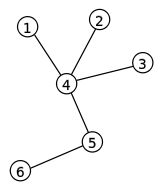
\includegraphics[height = 5cm,width = 4cm]{prufer.png}\\
上面的树结构可得普吕弗序列:{4,4,4,5}。

\subsection{从普吕弗序列还原无根树}
设这普吕弗序列长$n − 2$。首先写出数1至$n$。第一步,找出1至$n$中没有在序列中出现的最小数。把标号为这数的顶点和标号为序列首项的顶点连起来,并把这数从1至$n$中删去,序列的首项也删去。接着每一步以1至$n$中剩下的数和余下序列重复以上步骤。最后当序列用完,把1至n中最后剩下的两数的顶点连起来。

\subsection{结论}
\begin{itemize}
\item 一个长为$n−2$且每项都在1至$n$之间的序列$S$,有唯一的标号树以$S$为普吕弗序列。
\item 长$n−2$的序列共有$n^{n−2}$个,从而证明凯莱公式:$n$顶点的标号无根树共有$n^{n−2}$棵。
\item 一棵标号树实际上是标号完全图的一棵生成树。对普吕弗序列加以限制。类似的方法可以得到标号完全二分图的生成树总数。若$G$是完全二分图,一部分的顶点标号1到$n_1$,另一部分的顶点标号$n_{1} + 1$到$n$。$G$的标号生成树总数为,$n_{1}^{n_{2}-1}*n_{2}^{n_{1}-1}$其中$n_{2} = n − n_1$。
\item 普吕弗序列中某个编号$i$出现的次数$=d(i)-1,d(i)$是这个编号的节点在无根树中的度数
\item $n$个节点的度依次为$d_1, d_2,\cdots , d_n$的无根树共有 $ \frac{(n-2)!} {[ (d_1-1)!*(d_2-1)!*\cdots *(d_n-1)! ] }$个,因为此时$Prufer$编码中的数字$i$恰好出现$d_i-1$次。
\item $n$个节点的度依次为$d_1, d_2,\cdots , d_n$,另有$m$个节点度数未知,求有多少种生成树?[BZOJ1005 明明的烦恼]令每个已知度数的节点的度数为$d_i(i:1\sim k)$,有$n$个节点,$m$个节点未知度数,$sum=\sum_{i=1}^{k}(d(i)-1)$。
$$
Ans=C_{n-2}^{sum}*\frac{sum!}{\prod_{i=1}^{k}(d(i)-1)!}*(n-k)^{n-sum-2}
$$

\item $n$个点的有标号有根树的计数:$n^{n-2}*n = n^{n-1}$
\end{itemize}
\subsection{BZOJ 1211}
给定一棵$n\leq 150$个结点的树中所有点的度数,求有多少种可能的树? \\
直接乘会爆long long,所以先把每个数分解质因数,把质因数的次数相加相减,然后再乘起来。无解需要输出0。当$n!=1\&\&d[i]==0$时或者当$\sum(d[i]-1)!=n-2$时无解。
\begin{lstlisting}
int n, sum = 0;
int num[200];

ll Qpow(int a, int b) {
    ll ret = 1, t = a;
    while (b) {
        if (b & 1) ret *= t;
        t *= t;
        b >>= 1;
    }
    return ret;
}

void update(int x, int flag) {
    for (int i = 2; i * i <= x; ++i) {
        while (x % i == 0) num[i] += flag, x /= i;
    }
    if (x > 1) num[x] += flag;
}

int main() {
    scanf("%d", &n);
    for (int i = 2; i <= n - 2; ++i) update(i, 1);
    for (int i = 1; i <= n; ++i) {
        int d;
        scanf("%d", &d);
        if (d == 0 && n > 1) {
            printf("0\n");
            return 0;
        }
        sum += d;
        for (int j = 2; j <= d - 1; ++j) update(j, -1);
    }
    if (sum != 2 * n - 2) printf("0\n");
    else {
        ll ans = 1;
        for (int i = 2; i <= n; ++i) {
            if (num[i]) ans *= Qpow(i, num[i]);
        }
        printf("%lld\n", ans);
    }
    return 0;
}
\end{lstlisting}
\subsection{HDU 5629}
给$n\leq 50$个点,每个结点的度数不超过$a_i\in [1,n]$,求构造树大小(结点个数)为$s\in [1,n]$的方案数,答案对$1e9+7$取模。\\

用$dp[i][j][k]$表示处理到第$i$个节点,从中选择$j$个节点,且可重集大小(普吕弗序列长度)为$k$的排列组合数。初始化$dp[0][0][0]=1$,考虑用$dp[i-1][j][k]$来更新$dp[i][][]$的状态:不用第$i$个结点和枚举第$i$个结点的度数。滚动数组实现。\\

时间复杂度:$O(n^4)$,可以使用$FFT$优化到$O(n^3\log n)$,但是因为常数原因,差别不大。
\begin{lstlisting}
const int MAX_N = 55;
const ll mod = (ll)(1e9) + 7;

int T, n;
int a[MAX_N];
ll dp[2][MAX_N][MAX_N], C[MAX_N][MAX_N];

int main() {
    for (int i = 0; i < MAX_N; ++i) {
        C[i][0] = C[i][i] = 1;
        for (int j = 1; j < i; ++j) {
            C[i][j] = (C[i - 1][j] + C[i - 1][j - 1]) % mod;
        }
    }
    scanf("%d", &T);
    while (T--) {
        scanf("%d", &n);
        for (int i = 1; i <= n; ++i) scanf("%d", &a[i]);
        memset(dp, 0, sizeof (dp));
        dp[0][0][0] = 1;
        int now = 0;
        for (int i = 1; i <= n; ++i) {
            now ^= 1;
            memset(dp[now], 0, sizeof (dp[now]));
            for (int j = 0; j <= i; ++j) {
                for (int k = 0; k <= n - 2; ++k) {
                    dp[now][j][k] += dp[now ^ 1][j][k];
                    if (dp[now][j][k] >= mod) dp[now][j][k] -= mod;
                    for (int p = 1; p <= a[i] && k + p - 1 <= n - 2; ++p) {
            dp[now][j + 1][p + k - 1] += dp[now ^ 1][j][k] * C[k + p - 1][p - 1] % mod;
            if (dp[now][j + 1][p + k - 1] >= mod) dp[now][j + 1][p + k - 1] -= mod;
                    }
                }
            }
        }
        printf("%d", n);
        for (int j = 2; j <= n; ++j) printf(" %lld", dp[now][j][j - 2]);
        printf("\n");
    }
    return 0;
}
\end{lstlisting}

%\end{document}

%\documentclass[UTF8]{book} % 使用book文档类型格式排版
\usepackage{ctex}  %加载包,因为我们在用中文写文档,所以必须加载这个包,否则不支持中文

%加入了一些针对XeTeX的改进并且加入了 \XeTeX 命令来输入漂亮的XeTeX logo
\usepackage{xltxtra}
%启用一些LaTeX中的功能
\usepackage{xunicode}

\usepackage{multicol}  %加载包
\usepackage{amsmath} % 调用公式宏包
\usepackage{amssymb} % 数学符号生成命令
\usepackage{array} % 数组和表格制作
\usepackage{booktabs} % 绘制水平表格线
\usepackage{calc} %四则运算
\usepackage{caption} % 插图和表格标题格式设置
\usepackage{fancyhdr} % 页眉页脚设置
\usepackage{graphicx} % 调用插图宏包
\usepackage{multicol} % 多栏排版
\usepackage{titlesec} % 章节标题格式设置

%%%% 目录样式 %%%%
\usepackage{titletoc}
\titlecontents{chapter}[1pt]{\vspace{.5\baselineskip}\bfseries}
    {{\thecontentslabel}\quad}{}
    {\hspace{.5em}\titlerule*[10pt]{$\cdot$}\contentspage}
\titlecontents{section}[2em]{\vspace{.25\baselineskip}\bfseries}
    {\thecontentslabel\quad}{}
    {\hspace{.5em}\titlerule*[10pt]{$\cdot$}\contentspage}

\usepackage{color}
\usepackage{xcolor} % 颜色处理
%\usepackage{indentfirst} % 自动首行缩进
%\setlength{\parindent}{2.22em} % 设置首行缩进的距离
% 设置超链接颜色
\usepackage[colorlinks=true,linkcolor=black,urlcolor=black,citecolor=black]{hyperref} % 根据章节标题生成PDF书签

%%%% 版面 %%%%
\usepackage[top=0.5in,bottom=0.5in,left=1.25in,right=0.8in]{geometry}
% 设置行距
\linespread{1}
\usepackage{lscape}
\usepackage{listings} %插入代码,代码页需要加入[fragile]
\usepackage{xeCJK}

%\usepackage[slantfont,boldfont]{xeCJK} % 允许斜体和粗体

%%%% fontspec 宏包 %%%%
\usepackage{fontspec}
% 指定字体
%\setmonofont[Mapping={}]{Monaco}	%英文引号之类的正常显示,相当于设置英文字体
%\setsansfont{Monaco} %设置英文字体 Monaco, Consolas,  Fantasque Sans Mono
%\setmainfont{Monaco} %设置英文字体
% \setCJKmainfont{方正兰亭黑简体}  %中文字体设置
% \setCJKsansfont{华康少女字体} %设置中文字体
% \setCJKmonofont{华康少女字体} %设置中文字体

%%%%%%%%%% 图形支持宏包 %%%%%%%%%%
\usepackage{graphicx}                % 嵌入png图像
\usepackage{color,xcolor}            % 支持彩色文本、底色、文本框等
%\usepackage{subfigure}
%\usepackage{epsfig}                 % 支持eps图像
%\usepackage{picinpar}               % 图表和文字混排宏包
%\usepackage[verbose]{wrapfig}       % 图表和文字混排宏包
%\usepackage{eso-pic}                % 向文档的部分页加n副图形, 可实现水印效果
%\usepackage{eepic}                  % 扩展的绘图支持
%\usepackage{curves}                 % 绘制复杂曲线
%\usepackage{texdraw}                % 增强的绘图工具
%\usepackage{treedoc}                % 树形图绘制
%\usepackage{pictex}                 % 可以画任意的图形
%\usepackage{hyperref}

%\setCJKmainfont{Kai}   % 设置缺省中文字体
%\setCJKmonofont{Hei}   % 设置等宽字体
%\setmainfont{Optima}   % 英文衬线字体
%\setmonofont{Monaco}   % 英文等宽字体
%\setsansfont{Trebuchet MS} % 英文无衬线字体

\makeatletter
\providecommand*\input@path{}
\newcommand\addinputpath[1]{
\expandafter\def\expandafter\input@path
\expandafter{\input@path{#1}}}
\addinputpath{body/}
\makeatother

\definecolor{keywordcolor}{rgb}{0.8,0.1,0.5}
\lstset{language=C++, %用于设置语言为C++
    numbers=left, %设置行号位置
    numberstyle=\tiny, %设置行号大小
    keywordstyle=\color{keywordcolor} \bfseries,
    identifierstyle=,
    basicstyle=\ttfamily,
    commentstyle=\color{blue} \textit, %注释颜色
    stringstyle=\ttfamily,
    showstringspaces=false,
    frame=shadowbox, %边框
    %frame = single,
    tabsize=2, %设置tab空格数
    showspaces=false, %不显示空格
    escapeinside=``, %逃逸字符(1左面的键),用于显示中文
    %breaklines, %自动折行
    captionpos=b
}

%\begin{document}

\chapter{字符串}

\section{KMP}
[HDU 1867]: 求两个字符串相加之后的最短长度。(首尾可重叠消去,两个字符串的长度$\leq 10^5$)。\\
也可以哈希做。
\begin{lstlisting}
#include <bits/stdc++.h>
using namespace std;

string s1, s2;
int nxt[100010];

string solve(string S1, string S2) {
    int n = S1.length(), m = S2.length();
    nxt[0] = nxt[1] = 0;

    int j = 0;
    for (int i = 1; i < m; ++i) {
        while (j && S2[i] != S2[j]) j = nxt[j];
        if (S2[i] == S2[j]) ++j;
        nxt[i + 1] = j;
    }

    j = 0;
    for (int i = 0; i < n; ++i) {
        while (j && S1[i] != S2[j]) j = nxt[j];
        if (S1[i] == S2[j]) ++j;
    }

    string ret(S1);
    for (int i = j; i < m; ++i) ret += S2[i];
    return ret;
}

int main() {
    while (cin >> s1 >> s2) {
        string ans1 = solve(s1, s2);
        string ans2 = solve(s2, s1);
        int len1 = ans1.length(), len2 = ans2.length();
        if (len1 < len2 || (len1 == len2 && ans1 < ans2))
            cout << ans1 << endl;
        else
            cout << ans2 << endl;
    }
    return 0;
}
\end{lstlisting}

\clearpage
\section{Shift-And算法}

基于位并行的算法,如Shift-And算法的基本思想是:将模式串集合与文本串的匹配状态用位向量存储,匹配过程就是用位操作更新位向量的过程。它的优点是所需存储空间小,匹配速度快;缺点是算法性能会随模式串个数的增多而下降,只适合中小规模的模式串集合。\\

Shift-And算法维护一个字符串的集合,集合中的每个字符串既是模式串$p$的前缀,同时也是已读入文本的后缀。每读入一个新的文本字符,该算法采用位并行的方法更新该集合,该集合用一个位掩码$D=d_{m}...d_1$来表示。$D$的第$j$位被置为1,当且仅当$p_{1}…p_{j}$是$t_{1}…t_{i}$的后缀。 \\

Shift-And算法首先构造一个$m$位($m$是模式串的长度)的向量表$B[]$,用来记录字符在模式串的出现位置。如果$p_j$为字符$c$,掩码$B[c]$的第$j$位被置为1,否则为0。首先置$D=0^m$,对于每个新读入的文本字符$t_{i+1}$,用如下公式对$D$进行更新:$D[i+1]=((D[i]<<1)|0^{m+1}1)\&B[t_{i+1}]$。在匹配时,逐个扫描文本字符并更新向量$D$,当$D[i]\&10^{m-1}≠0^{m}$时,在文本位置$i$处匹配成功。 \\

Shift-And算法扩展到多模式串时,将所有模式串的位向量$D$包装到一个机器字里,用位并行技术同时对$r$个位向量进行更新,初始化字和匹配掩码分别是所有初始化字和所有匹配掩码的连接。 \\

设机器字的长度为$w$,文本串的长度为$n$,模式串的个数为$r$,最短模式串长度为$m$,那么Shift-And算法的时间复杂度为$O(n\lceil \frac{m*r}{w}\rceil)$。由于采用了位并行技术,Shift-And算法的匹配速度是很快的。但一旦模式串的长度和超出机器字的长度,算法的性能都会发生明显下降。\\
\underline{[2016 大连B]} \\

给一个$n\leq 1000$,代表数字长度,以及每位上候选数字集合,再给一个数字字符串$s(|s|\leq 5*10^{6})$,输出$s$中所有匹配的$n$位数字子串。\\
样例输入:\\
4 (一共四位) \\
3 0 9 7 (第一位有三个候选数字分别为:0 9 7) \\
2 5 7   (第二位有两个候选数字分别为:5 7) \\
2 2 5   (第三位有两个候选数字分别为:2 5) \\
2 4 5   (第四位有两个候选数字分别为:4 5) \\
09755420524 (数字字符串s) \\
样例输出:(所有匹配的四位数字子串) \\
9755 \\
7554 \\
0524 \\

\begin{lstlisting}
#include <inttypes.h>

const int MAX_N = 1005;
const int MAX_LEN = 10000005;
const int MAX_ARR_LEN = ((MAX_N >> 6) + 5);
const int MASK = 63;

int n;
ll num[10][MAX_ARR_LEN], ret_n[MAX_ARR_LEN];
ll ind_x_arr[MAX_N], ind_y_arr[MAX_N];
char str[MAX_LEN];

void init() {
	memset(num, 0, sizeof (num));
	memset(ret_n, 0, sizeof (ret_n));
	for (int i = 0; i < n; ++i) {
		ind_x_arr[i] = (i >> 6) + 1; // i 位置属于哪一段
		ind_y_arr[i] = 1ll << (i & MASK); // 二进制中对应的位置
	}
}

inline void set_one(ll *arr, int pos) {
	arr[ind_x_arr[pos]] |= ind_y_arr[pos];
}

inline bool seek_one(ll *arr, int pos) {
	return arr[ind_x_arr[pos]] & ind_y_arr[pos];
}

inline void left_move_one(ll *arr, int pos) {
	for (int i = pos; i >= 1; --i) {
		arr[i] <<= 1;
		arr[i] |= (!!(arr[i - 1] & 0x8000000000000000ll));
	}
	set_one(arr, 0);
}

inline void and_opt(ll *arr1, ll *arr2, int pos) {
	for (int i = 1; i <= pos; ++i) {
		arr1[i] &= arr2[i];
	}
}

int main() {
	scanf("%d", &n);
	init();
	for (int i = 0; i < n; ++i) {
		int x, y;
		scanf("%d", &x);
		for (int j = 0; j < x; ++j) {
			scanf("%d", &y);
			set_one(num[y], i);
		}
	}
	scanf("%s", str);
	int len = strlen(str);
	int L = n >> 6;
	if (n & MASK) L++; // 分成若干段数
	for (int i = 0; i < len; ++i) {
		left_move_one(ret_n, L);
		and_opt(ret_n, num[str[i] - '0'], L);
		if (seek_one(ret_n, n - 1)) {
			char ch = str[i + 1];
			str[i + 1] = '\0';
			printf("%s\n", str + i - n + 1);
			str[i + 1] = ch;
		}
	}
	return 0;
}
\end{lstlisting}

\clearpage
\section{字典树}
\subsection{HDU 1857}

给出一个$n*m(n,m\in [20,500])$的字母表,对每个询问串输出它在字母表中的位置。可以从某个位置一直向右,一直向右下查找或者一直向下,输出最左上的起始位置。查找不到输出$(-1,-1)$。

先把所有的询问串创建字典树,然后扫描字母表,看字母表中的串是否有在字典树中出现。
\begin{lstlisting}
const int MAX = 1000010;
const int NUM = 26;
const int dir[4][2] = {{0, 1}, {1, 1}, {1, 0}};

int n, m;
int child[MAX][NUM], bel[MAX];
char mat[510][510];
pair<int, int> ans[10010];

struct Trie {
    int tot, root;

    void init() {
        memset(child[1], 0, sizeof (child[1]));
        tot = root = 1; bel[1] = 0;
    }
    void insert(const char* str, const int id) {
        int* cur = &root;
        for (const char* p = str; *p; ++p) {
            cur = &child[*cur][*p - 'A'];
            if (*cur == 0) {
                *cur = ++tot;
                memset(child[tot], 0, sizeof (child[tot]));
                bel[tot] = 0;
            }
        }
        bel[*cur] = id;
    }
    void query(const int x, const int y, const int id) {
        int step = 0, tmpx = x, tmpy = y;
        int* cur = &root;
        while (1) {
            if (step > 20 || tmpx >= n || tmpy >= m) return;
            char ch = mat[tmpx][tmpy];
            cur = &child[*cur][ch - 'A'];
            if (*cur == 0) return;
            int pos = bel[*cur];
            if (pos != 0 && ans[pos].first == -1) ans[pos] = make_pair(x, y);
            tmpx += dir[id][0], tmpy += dir[id][1];
            step++;
        }
    }
} dic;

int main() {
    scanf("%d%d", &n, &m);
    for (int i = 0; i < n; ++i) scanf("%s", mat[i]);
    char str[20];
    getchar(); getchar();
    int num = 0;
    dic.init();
    while (gets(str) && str[0] != '-') {
        dic.insert(str, ++num);
        ans[num] = make_pair(-1, -1);
    }
    for (int i = 0; i < n; ++i) {
        for (int j = 0; j < m; ++j) {
            for (int k = 0; k < 3; ++k) {
                dic.query(i, j, k);
            }
        }
    }
    for (int i = 1; i <= num; ++i) printf("%d %d\n", ans[i].first, ans[i].second);
    return 0;
}
\end{lstlisting}

\subsection{HDU 5536}

给$n\leq 1000$个$\leq 1e9$的正整数$a_i$,从中找到三个互不相同的$a_i,a_j,a_k$使得$(a_i+a_j)\otimes a_k$最大。输出最大值。$\otimes$表示异或。

把所有$a_i$从高位开始插进字典树,贪心查找。再支持一个删除操作就可以了,因为要保证互不相同。

时间复杂度:$O(n^2 * 30)$,再乘上一个微小的常数。
\begin{lstlisting}
const int MAX = 1000010;
const int NUM = 2;
const int MAX_N = 1010;

int child[MAX][NUM], cnt[MAX];

struct Trie {
    int root, tot;

    void init() {
        root = tot = 1;
        child[1][0] = child[1][1] = 0;
        cnt[1] = 1;
    }
    void insert(const int x) {
        int* cur = &root;
        for (int i = 30; i >= 0; --i) {
            cur = &child[*cur][(x >> i) & 1];
            if (*cur == 0) {
                *cur = ++tot;
                child[tot][0] = child[tot][1] = 0;
                cnt[tot] = 0;
            }
            cnt[*cur]++;
        }
    }
    void remove(const int x) {
        int* cur = &root;
        for (int i = 30; i >= 0; --i) {
            cur = &child[*cur][(x >> i) & 1];
            cnt[*cur]--;
        }
    }
    int query(const int x) {
        int ret = 0;
        int* cur = &root;
        for (int i = 30; i >= 0; --i) {
            int now = (x >> i) & 1, store = *cur;
            if (now == 0) {
                cur = &child[*cur][1];
                if (cnt[*cur]) ret += (1 << i);
                else cur = &child[store][0];
            } else {
                cur = &child[*cur][0];
                if (cnt[*cur]) ret += (1 << i);
                else cur = &child[store][1];
            }
        }
        return ret;
    }
} dic;

int T, n;
int a[MAX_N];

int main() {
    scanf("%d", &T);
    while (T--) {
        scanf("%d", &n);
        dic.init();
        for (int i = 1; i <= n; ++i) {
            scanf("%d", &a[i]);
            dic.insert(a[i]);
        }
        int ans = 0;
        for (int i = 1; i <= n; ++i) {
            dic.remove(a[i]);
            for (int j = i + 1; j <= n; ++j) {
                dic.remove(a[j]);
                ans = max(ans, dic.query(a[i] + a[j]));
                dic.insert(a[j]);
            }
            dic.insert(a[i]);
        }
        printf("%d\n", ans);
    }
    return 0;
}
\end{lstlisting}

%\end{document}


\end{document}
